% \iffalse
%  Local Variables:
%  mode: doctex
%  TeX-master: t
%  End:
% \fi
%
% \iffalse meta-comment
%
% Copyright (C) 2005-2013 by Ruini Xue <xueruini@gmail.com>
%
% This file may be distributed and/or modified under the
% conditions of the LaTeX Project Public License, either version 1.3a
% of this license or (at your option) any later version.
% The latest version of this license is in:
%
% http://www.latex-project.org/lppl.txt
%
% and version 1.3a or later is part of all distributions of LaTeX
% version 2004/10/01 or later.
%
% $Id$
%
% \fi
%
% \CheckSum{0}
% \CharacterTable
%  {Upper-case    \A\B\C\D\E\F\G\H\I\J\K\L\M\N\O\P\Q\R\S\T\U\V\W\X\Y\Z
%   Lower-case    \a\b\c\d\e\f\g\h\i\j\k\l\m\n\o\p\q\r\s\t\u\v\w\x\y\z
%   Digits        \0\1\2\3\4\5\6\7\8\9
%   Exclamation   \!     Double quote  \"     Hash (number) \#
%   Dollar        \$     Percent       \%     Ampersand     \&
%   Acute accent  \'     Left paren    \(     Right paren   \)
%   Asterisk      \*     Plus          \+     Comma         \,
%   Minus         \-     Point         \.     Solidus       \/
%   Colon         \:     Semicolon     \;     Less than     \<
%   Equals        \=     Greater than  \>     Question mark \?
%   Commercial at \@     Left bracket  \[     Backslash     \\
%   Right bracket \]     Circumflex    \^     Underscore    \_
%   Grave accent  \`     Left brace    \{     Vertical bar  \|
%   Right brace   \}     Tilde         \~}
%
% \iffalse
%<*driver>
\ProvidesFile{thuthesis.dtx}[2012/07/28 4.8dev Tsinghua University Thesis Template]
\documentclass[10pt]{ltxdoc}
\usepackage{dtx-style}
\EnableCrossrefs
\CodelineIndex
\RecordChanges
%\OnlyDescription
\begin{document}
  \DocInput{\jobname.dtx}
\end{document}
%</driver>
% \fi
%
% \GetFileInfo{\jobname.dtx}
% \MakeShortVerb{\|}
%
% \def\thuthesis{\textsc{Thu}\-\textsc{Thesis}}
% \def\pkg#1{\texttt{#1}}
%
% \changes{v1.0-}{2005/07/06}{Please refer to ``Bao--Pan'' version.}
%
% \changes{v1.1}{2005/11/03}{Initial version, migrate from the old ``Bao--Pan''
% version. Make the template a class instead of package.}
%
% \changes{v1.2}{2005/11/04}{Remove \textbf{fancyref}; Remove \textbf{ucite} and implemente
% \textbf{onlinecite}; use package arial or helvet selectively.}
%
% \changes{v1.3}{2005/11/14}{replace subfigure with subfig, replace caption2
% with caption, add details about using figure in the example.}
%
% \changes{v1.4rc1}{2005/11/20}{I do not why \textbf{thu@authorizationaddon} does not work
% now for v1.3, while it's fine in v1.2. Temporarily, I remove the directive
% :(. There might be nicer solution. Other changes: add \textsf{config} option to
% subfig to be compatible with subfigure. add \textbf{courier} package for tt font.}
%
% \changes{v1.4}{2005/12/05}{Fix the problem of \textbf{chinese}, that is
% because both CJK and everysel redefined the \textbf{selectfont}. So, a not so good
% workaround is merge them up. Add \textbf{shuji} example. Add \textbf{pozhehao} command.}
%
% \changes{v2.1}{2006/02/27}{Add support to bachelor thesis.}
% \changes{v2.1}{2006/03/01}{Remove \pkg{fancyhdr} and \pkg{geometry}.}
% \changes{v2.1}{2006/03/01}{Redefine footnote marks.}
% \changes{v2.1}{2006/03/01}{Replace thubib.bst with chinesebst.bst.}
% \changes{v2.1}{2006/03/02}{Merge the modification of \pkg{ntheorem}.}
% \changes{v2.1}{2006/03/02}{Remove \pkg{footmisc} and refine the document.}
% \changes{v2.1}{2006/03/03}{Work very hard on the document.}
% \changes{v2.1}{2006/03/03}{Add |checklab| code to reduce ``unresolved labels'' warning}
% \changes{v2.2}{2006/03/26}{Adjust margins. How bad it is to simulate MS WORD!.}
% \changes{v2.2}{2006/03/26}{Add bachelor training overview details supporting.}
% \changes{v2.2}{2006/03/26}{CJK support in preamble.}
% \changes{v2.2}{2006/03/26}{Adjust hyperref to avoid boxes around links.}
% \changes{v2.3}{2006/04/07}{Fix a great bug: \cmd{PassOptionsToClass} and \cs{LoadClass}
% rather than \cs{PassOptionToPackage} and \cs{LoadPackage}.}
% \changes{v2.3}{2006/04/07}{Reorganize the codes in cover, make the pagestyle more readable.}
% \changes{v2.3}{2006/04/07}{Add gbk2uni into the document.}
% \changes{v2.3}{2006/04/07}{Support openright and openany.}
% \changes{v2.3}{2006/04/09}{Adjust hypersetup to remove color and box.}
% \changes{v2.3}{2006/04/09}{Adjust margins again.}
% \changes{v2.3}{2006/04/09}{Adjust references formats.}
% \changes{v2.3}{2006/04/09}{Redefine frontmatter and mainmatter to fit our case.}
% \changes{v2.3}{2006/04/09}{Add assumption environment.}
% \changes{v2.3}{2006/04/09}{Change the brace in the cover.}
% \changes{v2.4}{2006/04/14}{Fill more pdf info. with hypersetup.}
% \changes{v2.4}{2006/04/14}{自动隐藏密级为内部时后面的五角星。}
% \changes{v2.4}{2006/04/14}{增加``注释(Remark)''环境。}
% \changes{v2.4}{2006/04/14}{压缩 item 之间的距离。}
% \changes{v2.4}{2006/04/14}{thubib.bst 文献标题取消自动小写。}
% \changes{v2.4}{2006/04/14}{中文参考文献取消 In: Proceedings。}
% \changes{v2.4}{2006/04/14}{英文文参考文献调整 In: editor, Proceedings。}
% \changes{v2.4}{2006/04/14}{参考文献为学位论文时,加方括号,作者后面为实心点。}
% \changes{v2.4}{2006/04/14}{中文参考文献作者超过三个加等。}
% \changes{v2.4}{2006/04/14}{中文参考文献需要在 bib 中指定 |lang="chinese"|。}
% \changes{v2.4}{2006/04/14}{学位论文不在需要 type 字段。}
% \changes{v2.4}{2006/04/14}{为摘要等条目增加书签。}
% \changes{v2.4}{2006/04/14}{章节的编号用黑体,也就是自动打开 arialtitle 选项。}
% \changes{v2.4.1}{2006/04/17}{2.4 忘了把关键词的 tabular 改成 thu@tabular。}
% \changes{v2.4.1}{2006/04/17}{参考文献最后一个作者前是逗号而不是 and。}
% \changes{v2.4.2}{2006/04/18}{去掉参考文献第二个作者后面烦人的逗号。}
% \changes{v2.5}{2006/05/19}{对本科论文进行大幅度的重写,因为教务处修改了格式要求。}
% \changes{v2.5}{2006/05/19}{重新整理代码,使其布局更易读。}
% \changes{v2.5.1}{2006/05/24}{根据教务处的新要求调整附录部分。}
% \changes{v2.5.1}{2006/05/25}{参考文献中杂志文章如果没有卷号,那么页码直接跟在
% 年份后面,并用句点分割。在 thubib.bst 中增加 output.year 函数。}
% \changes{v2.6.1}{2006/06/16}{取消 thubib.bst 中 inbook 类 volume 后的页码。}
% \changes{v4.5}{2008/01/04}{彻底转向 UTF-8,并支持 xelatex。}
% \changes{v4.6}{2011/04/27}{增加博士后文档部分。}
% \changes{v4.6}{2011/10/22}{使用手册更新。}
% \changes{v4.7}{2012/06/12}{去掉 hypernat 依赖,hyperref 和 natbib 可以很好配合了。}
%
% \DoNotIndex{\begin,\end,\begingroup,\endgroup}
% \DoNotIndex{\ifx,\ifdim,\ifnum,\ifcase,\else,\or,\fi}
% \DoNotIndex{\let,\def,\xdef,\newcommand,\renewcommand}
% \DoNotIndex{\expandafter,\csname,\endcsname,\relax,\protect}
% \DoNotIndex{\Huge,\huge,\LARGE,\Large,\large,\normalsize}
% \DoNotIndex{\small,\footnotesize,\scriptsize,\tiny}
% \DoNotIndex{\normalfont,\bfseries,\slshape,\interlinepenalty}
% \DoNotIndex{\hfil,\par,\hskip,\vskip,\vspace,\quad}
% \DoNotIndex{\centering,\raggedright}
% \DoNotIndex{\c@secnumdepth,\@startsection,\@setfontsize}
% \DoNotIndex{\ ,\@plus,\@minus,\p@,\z@,\@m,\@M,\@ne,\m@ne}
% \DoNotIndex{\@@par,\DeclareOperation,\RequirePackage,\LoadClass}
% \DoNotIndex{\AtBeginDocument,\AtEndDocument}
%
% \IndexPrologue{\section*{索引}%
%    \addcontentsline{toc}{section}{索~~~~引}}
% \GlossaryPrologue{\section*{修改记录}%
%    \addcontentsline{toc}{section}{修改记录}}
%
% \renewcommand{\abstractname}{摘~~要}
% \renewcommand{\contentsname}{目~~录}
%
%
% \title{\thuthesis:清华大学学位论文模板\thanks{Tsinghua University \LaTeX{} Thesis Template.}}
% \author{{\fangsong 薛瑞尼\thanks{LittleLeo@newsmth}}\\[5pt]{\fangsong 清华大学计算机系高性能所}\\[5pt] \texttt{xueruini@gmail.com}}
% \date{v\fileversion\ (\filedate)}
% \maketitle\thispagestyle{empty}
%
%
% \begin{abstract}\noindent
%   此宏包旨在建立一个简单易用的清华大学学位论文模板,包括本科综合论文训练、硕士
%   论文、博士论文以及博士后出站报告。
% \end{abstract}
%
% \vskip2cm
% \def\abstractname{免责声明}
% \begin{abstract}
% \noindent
% \begin{enumerate}
% \item 本模板的发布遵守 \LaTeX{} Project Public License,使用前请认真阅读协议内容。
% \item 本模板为作者根据清华大学教务处颁发的《综合论文训练写作指南》,清华大学研
%   究生院颁发的《研究生学位论文写作指南》,清华大学《编写“清华大学博士后研究报告”参考意见》
%   编写而成,旨在供清华大学毕业生撰写学位论文使用。
% \item 清华大学教务处和研究生院只提供毕业论文写作指南,不提供官方模板,也不会授
%   权第三方模板为官方模板,所以此模板仅为写作指南的参考实现,不保证格式审查老师
%   不提意见。任何由于使用本模板而引起的论文格式审查问题均与本模板作者无关。
% \item 任何个人或组织以本模板为基础进行修改、扩展而生成的新的专用模板,请严格遵
%   守 \LaTeX{} Project Public License 协议。由于违犯协议而引起的任何纠纷争端均与
%   本模板作者无关。
% \end{enumerate}
% \end{abstract}
%
%
% \clearpage
% \begin{multicols}{2}[
%   \section*{\contentsname}
%   \setlength{\columnseprule}{.4pt}
%   \setlength{\columnsep}{18pt}]
%   \tableofcontents
% \end{multicols}
%
% \clearpage
% \pagenumbering{arabic}
% \pagestyle{headings}
% \section{模板介绍}
% \thuthesis\ (\textbf{T}sing\textbf{hu}a \textbf{Thesis}) 是为了帮助清华大学毕业
% 生撰写毕业论文而编写的 \LaTeX{} 论文模板。
%
% 本文档将尽量完整的介绍模板的使用方法,如有不清楚之处可以参考示例文档或者给邮件
% 列表(见后)写信,欢迎感兴趣的同学出力完善此使用手册。由于个人水平有限,虽然现
% 在的这个版本基本上满足了学校的要求,但难免还存在不足之处,欢迎大家积极反馈。
%
% {\color{blue}\fangsong 模板的作用在于减轻论文写作过程中格式调整的时间,其前提就是遵
%   守模板的用法,否则即使使用了 \thuthesis{} 也难以保证输出的论文符合学校规范。}
%
%
% \section{安装}
% \label{sec:installation}
%
% \subsection{下载}
% \thuthesis{} 相关链接:
% \begin{itemize}
% \item 主页:
% \href{https://github.com/xueruini/thuthesis}{GitHub}\footnote{已经从
% \url{http://thuthesis.sourceforge.net}迁移至此。}
% \item 下载:\href{http://code.google.com/p/thuthesis/}{Google Code}
% \item 同时本模板也提交至
% \href{http://www.ctan.org/macros/latex/contrib/thuthesis}{CTAN}
% \end{itemize}
% 除此之外,不再维护任何镜像。
%
% \thuthesis{} 的开发版本同样可以在 GitHub 上获得:
% \begin{shell}
% $ git clone git://github.com/xueruini/thuthesis.git
% \end{shell}
%
% \subsection{模板的组成部分}
% 下表列出了 \thuthesis{} 的主要文件及其功能介绍:
%
% \begin{center}
%   \begin{longtable}{l|p{10cm}}
% \hline
% {\heiti 文件(夹)} & {\heiti 功能描述}\\\hline\hline
% \endfirsthead
% \hline
% {\heiti 文件(夹)} & {\heiti 功能描述}\\\hline\hline
% \endhead
% \endfoot
% \endlastfoot
% thuthesis.ins & 模板驱动文件 \\
% thuthesis.dtx & 模板文档代码的混合文件\\
% thuthesis.cls & 模板类文件\\
% thuthesis.cfg & 模板配置文件\\
% thubib.bst & 参考文献样式文件\\\hline
% main.tex & 示例文档主文件\\
% shuji.tex & 书脊示例文档\\
% ref/ & 示例文档参考文献目录\\
% data/ & 示例文档章节具体内容\\
% figures/ & 示例文档图片路径\\
% thutils.sty & 为示例文档加载其它宏包\\\hline
% Makefile & self-explanation \\
% Readme & self-explanation\\
% \textbf{thuthesis.pdf} & 用户手册(本文档)\\\hline
%   \end{longtable}
% \end{center}
%
% 需要说明几点:
% \begin{itemize}
% \item \emph{thuthesis.cls} 和 \emph{thuthesis.cfg} 可以
%   由 \emph{thuthesis.ins} 和 \emph{thuthesis.dtx} 生成,但为了降低新
%   手用户的使用难度,故将 cls和 cfg 一起发布。
% \item 使用前认真阅读文档:\emph{thuthesis.pdf}.
% \end{itemize}
% 
% \subsection{准备工作}
% \label{sec:prepare}
% 本模板用到以下宏包:
%
% \begin{center}
% \begin{minipage}{1.0\linewidth}\centering
% \begin{tabular}{*{6}{l}}\hline
%   ifxetex & xunicode & CJK\footnote{版本要求:$\geq$ v4.8.1} & xeCJK & \pkg{CJKpunct} & \pkg{ctex} \\
%   array & booktabs & longtable  &  amsmath & amssymb & ntheorem \\
%   indentfirst & paralist & txfonts & natbib & hyperref & \\
%   graphicx & \pkg{subcaption} &
%   \pkg{caption}\footnote{版本要求:$\geq$2006/03/21 v3.0j} &
%   \pkg{thubib.bst} & &\\\hline
% \end{tabular}
% \end{minipage}
% \end{center}
%
% 这些包在常见的 \TeX{} 系统中都有,如果没有请到 \url{www.ctan.org} 下载。推
% 荐 \TeX\ Live。
%
%
% \subsection{开始安装}
% \label{sec:install}
%
% \subsubsection{生成模板}
% \label{sec:generate-cls}
% {\heiti 说明:默认的发行包中已经包含了所有文件,可以直接使用。如果对如何由 dtx 生
%   成模板文件以及模板文档不感兴趣,请跳过本小节。}
%
% 模板解压缩后生成文件夹 thuthesis-VERSION\footnote{VERSION 为版本号。},其中包括:
% 模板源文件(thuthesis.ins 和 thuthesis.dtx),参考文献样式 thubib.bst,示例文档
% (main.tex,shuji.tex,thutils.sty\footnote{我把可能用到但不一定用到的包以及一
%   些命令定义都放在这里面,以免 thuthesis.cls 过分臃
%   肿。},data/ 和 figures/ 和 ref/)。在使用之前需要先生成模板文件和配置文件
% (具体命令细节请参考 |Readme| 和 |Makefile|):
%
% \begin{shell}
% $ cd thuthesis-VERSION
% # 生成 thuthesis.cls 和 thuthesis.cfg
% $ latex thuthesis.ins
%
% # 下面的命令用来生成用户手册,可以不执行
% $ latex thuthesis.dtx
% $ makeindex -s gind.ist -o thuthesis.ind thuthesis.idx
% $ makeindex -s gglo.ist -o thuthesis.gls thuthesis.glo
% $ latex thuthesis.dtx
% $ latex thuthesis.dtx  % 生成说明文档 thuthesis.dvi
% \end{shell}
%
%
% \subsubsection{dvi$\rightarrow$ps$\rightarrow$pdf}
% \label{sec:dvipspdf}
% 很多用户对 \LaTeX{} 命令执行的次数不太清楚,一个基本的原则是多次运行 \LaTeX{}
% 命令直至不再出现警告。下面给出生成示例文档的详细过程(\# 开头的行为注释),首先
% 来看经典的 \texttt{dvi$\rightarrow$ps$\rightarrow$pdf} 方式:
% \begin{shell}
% # 1. 发现里面的引用关系,文件后缀 .tex 可以省略
% $ latex main
%
% # 2. 编译参考文件源文件,生成 bbl 文件
% $ bibtex main
%
% # 3. 下面解决引用
% $ latex main
% # 如果是 GBK 编码,此处运行:
% # $ gbk2uni main  # 防止书签乱码
% $ latex main   # 此时生成完整的 dvi 文件
%
% # 4. 生成 ps
% $ dvips main.dvi
%
% # 5. 生成 pdf
% $ ps2pdf main.ps
% \end{shell}
%
% 模板已经把纸型信息写入目标文件,这样执行 \texttt{dvips} 时就可以避免由于遗忘
%  \texttt{-ta4} 参数而导致输出不合格的文件(因为 \texttt{dvips} 默认使用
%  letter 纸型)。
%
% \subsubsection{dvipdfm(x)}
% \label{sec:dvipdfmx}
% 如果使用 dvipdfm(x),那么在生成完整的 dvi 文件之后(参见上面的例子),可以直接得到 pdf:
% \begin{shell}%
% $ dvipdfm  main.dvi
% # 或者
% $ dvipdfmx  main.dvi
% \end{shell}
%
% \subsubsection{pdflatex}
% \label{sec:pdflatex}
% 如果使用 PDF\LaTeX,按照第~\ref{sec:dvipspdf} 节的顺序执行到第 3 步即可,不再经
% 过中间转换。
%
% 需要注意的是 PDF\LaTeX\ 不能处理常见的 EPS 图形,需要先用 epstopdf 将其转化
% 成 PDF。不过 PDF\LaTeX\ 增加了对 png,jpg 等标量图形的支持,比较方便。
%
% \subsubsection{xelatex}
% \label{sec:xelatex}
% XeTeX 最大的优势就是不再需要繁琐的字体配置。\thuthesis{} 通过 \pkg{xeCJK} 来控
% 制中文字体和标点压缩。模板里默认用的是中易的四款免费字体(宋,黑,楷,仿宋),
% 用户可以根据自己的实际情况方便的替换。另外,本科论文封面要用到隶书,请用户自行
% 修改,参考第~\ref{sec:font-config} 节。
%
% Xe\LaTeX\ 的使用步骤同 PDF\LaTeX。
%
%
% \subsubsection{自动化过程}
% \label{sec:automation}
% 上面的例子只是给出一般情况下的使用方法,可以发现虽然命令很简单,但是每次都输入
% 的话还是非常罗嗦的,所以 \thuthesis{} 还提供了一些自动处理的文件。
%
% 我们提供了一个简单的 \texttt{Makefile}:
% \begin{shell}
% $ make clean
% $ make cls       # 生成 thuthesis.cls 和 thuthesis.cfg
% $ make doc       # 生成说明文档 thuthesis.pdf
% $ make thesis    # 生成示例文档 main.pdf
% $ make shuji     # 生成书脊 shuji.pdf
% \end{shell}
%
% \texttt{Makefile} 默认采用 Xe\LaTeX\ 编译,可以根据自己的
% 需要修改 \texttt{config.mk} 中的参数设置。
%
%
% \subsection{升级}
% \label{sec:updgrade}
% \thuthesis{} 升级非常简单,下载最新的版本,
% 将 thuthesis.ins,thuthesis.dtx 和thubib.bst 拷贝至工作目录覆盖相应的文件,然后
% 运行:
% \begin{shell}
% $ latex thuthesis.ins
% \end{shell}
%
% 生成新的类文件和配置文件即可。当然也可以直接拷贝 thuthesis.cls, thuthesis.cfg
% 和 thubib.bst,免去上面命令的执行。只要明白它的工作原理,这个不难操作。
%
%
% \section{使用说明}
% \label{sec:usage}
% 本手册假定用户已经能处理一般的 \LaTeX{} 文档,并对 \BibTeX{} 有一定了解。如果你
% 从来没有接触过 \TeX 和 \LaTeX,建议先学习相关的基础知识。磨刀不误砍柴工!
%
% \subsection{关于提问}
% \label{sec:howtoask}
% \begin{itemize}\addtolength{\itemsep}{-5pt}
% \item \url{http://groups.google.com/group/thuthesis}
% 或直接给\href{mailto:thuthesis@googlegroups.com}{邮件列表}写信。
% \item Google Groups mirror: \url{http://thuthesis.1048723.n5.nabble.com/}
% \item \href{http://www.newsmth.net/bbsdoc.php?board=TeX}{\TeX@newsmth}
% \end{itemize}
%
% \subsection{\thuthesis{} 使用向导}
% \label{sec:userguide}
% 推荐新用户先看网上的《\thuthesis{} 使用向导》幻灯片\footnote{有点老了,不过还是
%   很有帮助的。},那份讲稿比这份文档简练易懂。
%
% \subsection{\thuthesis{} 示例文件}
% \label{sec:userguide1}
% 模板核心文件只有三个:thuthesis.cls,thuthesis.cfg 和 thubib.bst,但是如果没有
% 示例文档用户会发现很难下手。所以推荐新用户从模板自带的示例文档入手,里面包括了
% 论文写作用到的所有命令及其使用方法,只需要用自己的内容进行相应替换就可以。对于
% 不清楚的命令可以查阅本手册。下面的例子描述了模板中章节的组织形式,来自于示例文
% 档,具体内容可以参考模板附带的 main.tex 和 data/。
%
% \begin{example}
% \documentclass[bachelor,nofonts]{thuthesis}
% %\documentclass[master,adobefonts]{thuthesis}
% %\documentclass[doctor]{thuthesis}
% %\documentclass[%
% %  bachelor|master|doctor|postdoctor, % 必选选项
% %  winfonts|nofonts|adobefonts, % 本科生、Linux 用户使用 XeLaTeX 时必选
% %  secret, % 可选选项
% %  openany|openright, % 可选选项
% %  arialtoc,arialtitle % 可选选项
% %  ]{thuthesis}
% % 当使用 XeLaTeX 编译时,本科生、Linux 用户需要加上 nofonts 选项;
% % 当使用 PDFLaTeX 编译时,adobefonts 选项等效于 winfonts 选项(缺省选项)。
%
% % 所有其它可能用到的包都统一放到这里了,可以根据自己的实际添加或者删除。
% \usepackage{thutils}
%
% % 可以在这里修改配置文件中的定义,导言区可以使用中文。
% % \def\myname{薛瑞尼}
%
% \begin{document}
%
% % 指定图片的搜索目录
% \graphicspath{{figures/}}
%
%
% %%% 封面部分
% \frontmatter
% 
%%% Local Variables:
%%% mode: latex
%%% TeX-master: t
%%% End:
\secretlevel{绝密} \secretyear{2100}

\ctitle{人体三维姿态估计算法研究}
% 根据自己的情况选,不用这样复杂
\makeatletter
\ifthu@bachelor\relax\else
  \ifthu@doctor
    \cdegree{工学博士}
  \else
    \ifthu@master
      \cdegree{工学硕士}
    \fi
  \fi
\fi
\makeatother


\cdepartment[自动化]{自动化系}
\cmajor{自动化}
\cauthor{梁鼎}
\csupervisor{刘烨斌副研究员}
% 如果没有副指导老师或者联合指导老师,把下面两行相应的删除即可。
%\cassosupervisor{陈文光教授}
%\ccosupervisor{某某某教授}
% 日期自动生成,如果你要自己写就改这个cdate
%\cdate{\CJKdigits{\the\year}年\CJKnumber{\the\month}月}

% 博士后部分
% \cfirstdiscipline{计算机科学与技术}
% \cseconddiscipline{系统结构}
% \postdoctordate{2009年7月——2011年7月}

\etitle{3D Human Pose Estimation}
% 这块比较复杂,需要分情况讨论:
% 1. 学术型硕士
%    \edegree:必须为Master of Arts或Master of Science(注意大小写)
%              “哲学、文学、历史学、法学、教育学、艺术学门类,公共管理学科
%               填写Master of Arts,其它填写Master of Science”
%    \emajor:“获得一级学科授权的学科填写一级学科名称,其它填写二级学科名称”
% 2. 专业型硕士
%    \edegree:“填写专业学位英文名称全称”
%    \emajor:“工程硕士填写工程领域,其它专业学位不填写此项”
% 3. 学术型博士
%    \edegree:Doctor of Philosophy(注意大小写)
%    \emajor:“获得一级学科授权的学科填写一级学科名称,其它填写二级学科名称”
% 4. 专业型博士
%    \edegree:“填写专业学位英文名称全称”
%    \emajor:不填写此项
\edegree{Bachelor of Automation}
\emajor{Automation}
\eauthor{Ding Liang}
\esupervisor{Associate Professor Yebin Liu}
%\eassosupervisor{Chen Wenguang}
% 这个日期也会自动生成,你要改么?
% \edate{December, 2005}

% 定义中英文摘要和关键字
\begin{cabstract}

人体姿态估计一直以来是计算机视觉研究领域的重点研究方向之一。人体姿态估计在体育运动分析、人机交互等领域有着广阔的应用前景和重大的应用价值。如今的研究主要集中于从单目图像中估计二维人体姿态信息,存在的问题有准确率低、无法完整刻画人体的运动姿态等。本文旨在通过从三幅不同角度拍摄的照片中估计出人体三维骨架信息。

本文的创新点有:
  \begin{itemize}
    \item 提出了一种有效的背景分割算法。原有的分割算法会产生很多空洞及毛边,这在HoG描述特征中会产生很大噪声,本文提出了一种有效的图像分割方法,使人物能从背景中完整分离;
    \item 提出了一种有效的HoG描述特征。原有的HoG特征维数过多,且会根据人物在图像中的尺寸改变每个元胞的大小,本文通过固定长宽比,保持了原有图像的信息;
    \item 提出了一种有效的含有皮肤信息的特征。新增的皮肤信息对姿态识别有重要帮助。
  \end{itemize}

综上所述,本文提出了一种新的图像特征描述,该特征能有效地应用于人体三维姿态估计中,显著降低了估计误差。

\end{cabstract}

\ckeywords{三维, 姿态, 估计}

\begin{eabstract}
   
\end{eabstract}

\ekeywords{$3$D, pose, estimation}

% \makecover
%
% % 目录
% \tableofcontents
%
% % 符号对照表
% \begin{denotation}

\item[HPC] 高性能计算 (High Performance Computing)
\item[cluster] 集群
\item[Itanium] 安腾
\item[SMP] 对称多处理
\item[API] 应用程序编程接口
\item[PI]	聚酰亚胺
\item[MPI]	聚酰亚胺模型化合物,N-苯基邻苯酰亚胺
\item[PBI]	聚苯并咪唑
\item[MPBI]	聚苯并咪唑模型化合物,N-苯基苯并咪唑
\item[PY]	聚吡咙
\item[PMDA-BDA]	均苯四酸二酐与联苯四胺合成的聚吡咙薄膜
\item[$\Delta G$]  	活化自由能~(Activation Free Energy)
\item [$\chi$] 传输系数~(Transmission Coefficient)
\item[$E$] 能量
\item[$m$] 质量
\item[$c$] 光速
\item[$P$] 概率
\item[$T$] 时间
\item[$v$] 速度
\item[劝  学] 君子曰:学不可以已。青,取之于蓝,而青于蓝;冰,水为之,而寒于水。
  木直中绳。(车柔)以为轮,其曲中规。虽有槁暴,不复挺者,(车柔)使之然也。故木
  受绳则直, 金就砺则利,君子博学而日参省乎己,则知明而行无过矣。吾尝终日而思
  矣,  不如须臾之所学也;吾尝(足齐)而望矣,不如登高之博见也。登高而招,臂非加
  长也,  而见者远;  顺风而呼,  声非加疾也,而闻者彰。假舆马者,非利足也,而致
  千里;假舟楫者,非能水也,而绝江河,  君子生非异也,善假于物也。积土成山,风雨
  兴焉;积水成渊,蛟龙生焉;积善成德,而神明自得,圣心备焉。故不积跬步,无以至千
  里;不积小流,无以成江海。骐骥一跃,不能十步;驽马十驾,功在不舍。锲而舍之,朽
  木不折;  锲而不舍,金石可镂。蚓无爪牙之利,筋骨之强,上食埃土,下饮黄泉,用心
  一也。蟹六跪而二螯,非蛇鳝之穴无可寄托者,用心躁也。\pozhehao{} 荀况
\end{denotation}

%
%
% %%% 正文部分
% \mainmatter
% 


\chapter{绪论}
本章首先阐述了本文研究问题提出的背景,并总结了前人的工作以及该研究方向的难点和重点,以此提出了自己研究的具体任务,最后简要介绍了本文的内容框架。

\section{研究背景}
过去的十到二十年以来,在计算机视觉领域很大比例的文章都与人物相关,包括人体检测与跟踪、人脸识别、人体姿态或动作的识别等等。前两个研究方向相对较为成熟,现在的算法已经可以很容易做到实时同时正确率超过90\%,然而人体姿态的识别却一直未能攻克。人们在图像中表达的信息很大程度上是由其姿态(即动作)决定的,因此人体姿态识别具有很广阔的应用前景,在人机交互、影视动画、临床运动诊断、体育运动动作分析等方面都有重要应用价值。例如微软公司设计的kinect传感器就可以实时捕捉识别人体的三维姿态,成功地应用于人机交互游戏中。

目前,最为流行且实用的人体姿态捕捉方法是利用多台摄像机、在目标人物身上附加标记点或传感器,这种方法在电影特效、游戏动画等领域应用十分普遍,被公认为是最有效的方法。这种方法的最大优点就是姿态能够准确获得,但它的问题有很多,使得该方法的应用受到了限制。基于标记点的方法对硬件设备依赖较大,标记点处理复杂,传感器价格昂贵,且无法对已有的图像或视频进行分析。因此,目前的研究都是为了摆脱标记点,用人工智能的方法自动检测识别人体姿态。本文也顺应该研究方向,力求提高识别精度。

\section{研究现状}
\subsection{综述}
人体姿态识别的研究内容有很多种分类方式,首先我们根据姿态描述信息的多少分为姿态估计和动作分类两种,动作分类的任务是给定一张静止图像或图像序列,判定这张图片中人物的动作类比,例如wang等人~\cite{wang2007semi}只需要分辨图像中人的动作是拳击、跑步或鼓掌等动作即可,而姿态估计则需要给出人物的关节点的具体位置来描述姿态,包含了更丰富的信息,以下将着重介绍姿态估计的相关研究。还有一种分类方式是依据是否需要人工参与分为全自动和半自动估计,wei等人~\cite{wei2009modeling}~\cite{wei2010videomocap}的工作就是在人工标定一些关键帧后由算法估计出其他视频帧中的任务姿态,以下的介绍将集中于全自动估计方法。此外还可以根据使用的图像视角的数量分为单目识别和多目识别,在二维姿态估计中只需要单目图像信息,三维姿态估计则通常需要多目信息,如~\cite{bo2008fast}~\cite{burenius20133d}~\cite{bo2010twin}~\cite{Poppe2007},但也有单目估计的算法,如~\cite{wei2009modeling}~\cite{wei2010videomocap}~\cite{agarwal2006recovering}。此外还可以分为单人和多人识别、二维和三维估计等。
\subsection{二维姿态估计算法}
\subsubsection{基于生成模型的姿态估计算法}
理想的生成模型应该能考虑到姿态、衣着的多样性,从而能生成更真实的样本,然而由于复杂度限制,这是不可能实现的。因此,人们做了很多假设,将场景限定在一定的范围内,缩小了样本空间。这类方法事先通过统计等方法给出一个人体姿态分布的先验函数,然后用似然函数描述观察到的图片所含姿态与先验函数姿态的一致性。这种方法的效果好坏很大程度上依赖于先验函数的优劣。

\subsubsection{基于判别模型的姿态估计算法}
判别模型方法不是事先给定先验函数,而是直接学习后验分布,这种方法与生成模型相比更加快捷、易于实现~\cite{gkiox2013ariarticulated}。

\subsubsection{基于肢体的姿态估计算法}
这种方法将身体分为各个部分,所有的肢体(如头、胳膊、腿等)构成一个集合,因此对完整姿态的估计从一个高维模型化简为若干个低维的推断问题,同样,为了使数学推断更行之有效,~\cite{felzenszwalb2005pictorial}~\cite{ferrari2008progressive}~\cite{ramanan2007learning} 做了一些简化和假设。多数基于肢体的方法本质上也是生成模型,但通常也包含了判别模型~\cite{andriluka2009pictorial}。\cite{yang2011articulated}取得了非常好的结果。

\subsubsection{其他算法}
Wang等人~\cite{wang2013beyond}使用了一种隐含树模型,通过学习各肢体间的关系,构建出一个树结构的图模型,在LSP~\cite{Johnson10LSP} 和PARSE~\cite{ramanan2007learning}数据集上得到了目前最优秀的结果。Tian等人~\cite{tian2012exploring}也使用了一种类似的树形结构,将人体分为三层,并用离散的类别刻画局部动作,取得了几乎是最好的结果。

\subsection{三维姿态估计算法}
\subsubsection{基于特征的姿态估计算法}
基于特征的方法本质上是基于判别模型的方法~\cite{agarwal2006local}~\cite{rosales2002learning}~\cite{shakhnarovich2003fast}~\cite{sminchisescu2005discriminative},输入图像被抽象成特征描述,经过学习得到模型,从而进行预测。代表性的几种方法有:Sminchisescu等人的SSLVM~\cite{bo2009SSLVM}、条件混合专家预测~\cite{bo2008fast}、双高斯过程~\cite{bo2010twin}。

\subsubsection{基于二维姿态估计的算法}
这种算法~\cite{burenius20133d}不关心二维姿态的估计,算法假定多视角的二维姿态已知,通过数据融合,推算出三维姿态,其强调的是如何将已有的二维姿态融合推广至三维情况。

\subsubsection{半自动姿态估计算法}
该算法~\cite{wei2009modeling}~\cite{wei2010videomocap}已在前文介绍,不再赘述。

\subsection{研究难点}
相关研究之所以未能取得很大突破,究其原因主要有如下几点,这些因素被公认为人体姿态估计领域的重要挑战。
\begin{enumerate}[(1)]
  \item 图像中人物外貌、衣着的多样性
  \item 光照条件的多样性
  \item 遮挡问题,包括自身肢体遮挡、他人或场景中物品对人物的遮挡
  \item 人体骨架的复杂性
  \item 人体姿态是一个高维描述
  \item \label{itm:3D}图片中丢失了3D信息
  \item 复杂的背景环境
\end{enumerate}
其中(\ref{itm:3D})在多目估计中不存在,因此多目图像估计能够更好地克服遮挡等问题。

\section{问题描述}
本文将研究内容聚焦于人体三维姿态的估计,具体说来,输入与输出如下:
\begin{description}
  \item[输入] 无标记的单目或多目静止图像(可以推广至图像序列)
  \item[输出] 用关节点表示的三维人体骨架(关于骨架表示法将在\ref{sec:skeleton}阐述)
\end{description}

可以参照图\ref{fig:inout}。

\begin{figure}[htbp]
    \centering
    \subcaptionbox{输入}{
    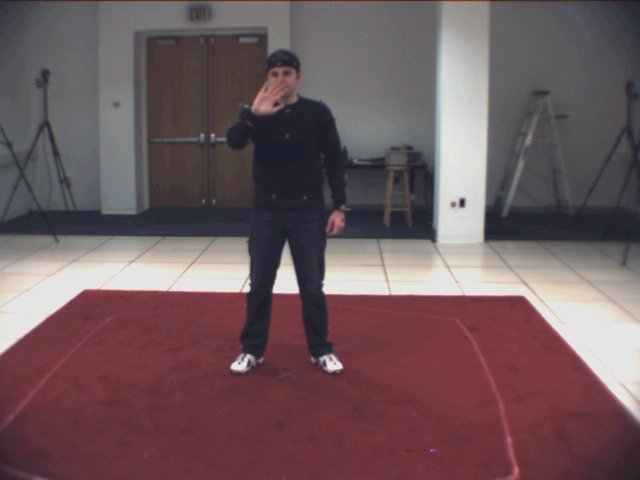
\includegraphics[height=6cm]{humaneva1.png}}
    \hspace{2cm}
    \subcaptionbox{输出}{
    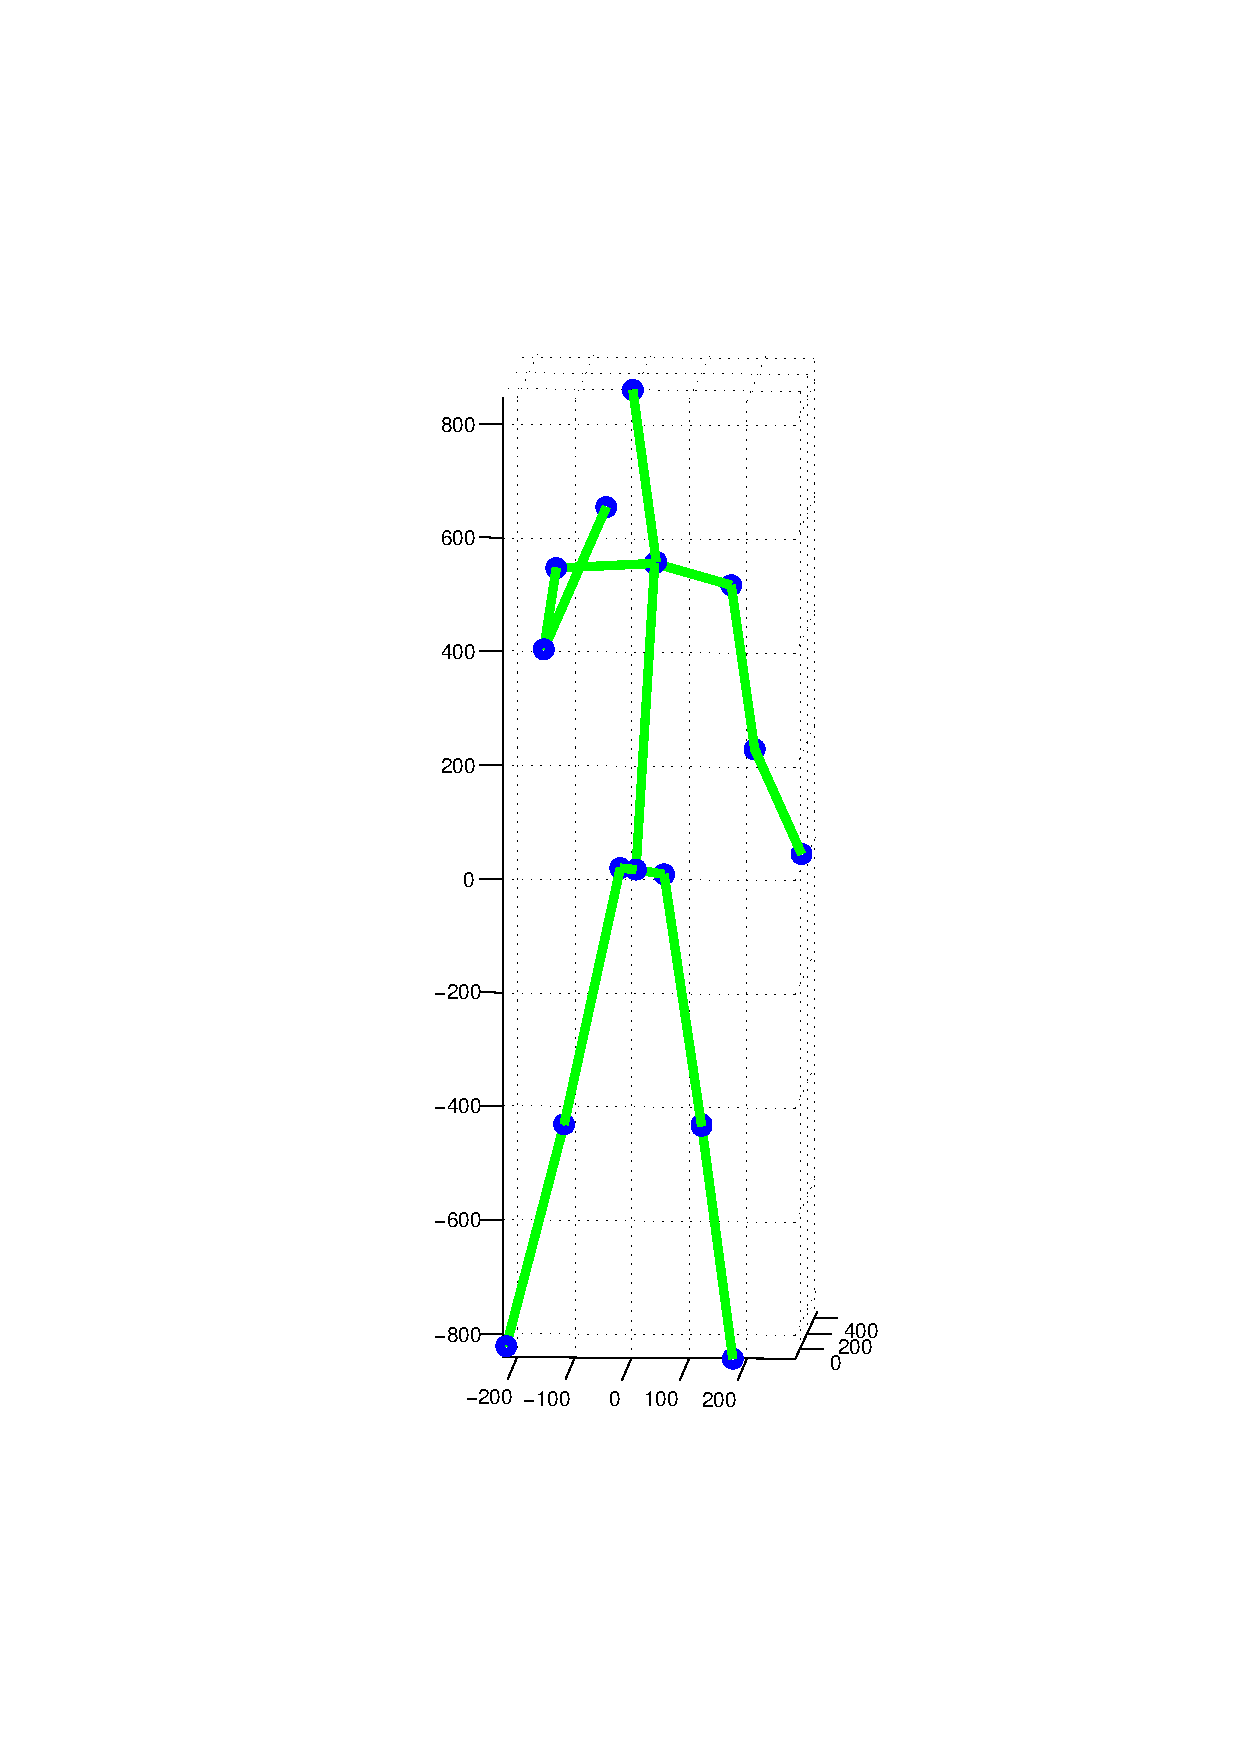
\includegraphics[height=6cm]{humaneva1_bone.pdf}}
    \caption{本文研究问题的输入与输出}
    \label{fig:inout}
\end{figure}


\section{文章结构}
本文共分为六章,第二章将介绍本人研究工作所依赖的数据库,包括数据库的内容、统计信息以及如何利用数据库等,其次介绍了本文所用的人体骨架模型的表示方法。第三章将介绍特征提取的一些方法,以及本文采用的特征以及其表示方法。第四章详细介绍了姿态估计算法,该算法基于双高斯过程,较好地考虑了输入输出变量之间的耦合关系。第五章主要以图表的方式整理了所做工作的结果,通过与前人工作对比,证明了本文工作的意义,并从结果中发现总结问题,分析可能的原因。第六章对全文做以总结,最后针对还存在的问题提出一些可能的解决方法和未来的努力方向。

% 


\chapter{构建三维人体姿态数据库}
由于人体姿态估计算法大部分为监督学习,因此研究者制作了很多用于训练和测试的数据库,这些数据库有些是从互联网、电影中获得的图片,并人工标记出骨架作为ground-truth,有些是通过标记点或传感器等手段在拍摄影像的同时记录人体姿态的ground-truth。表\ref{tab:benchmark}整理了目前常用的人体数据库,本文采用了HumanEva-I~\cite{sigal2006humaneva}数据库,将在\ref{sec:HumanEva}节介绍。

\begin{table}[htbp]
  \centering
  \renewcommand{\arraystretch}{1.5}
  \begin{minipage}[t]{\linewidth} % 如果想在表格中使用脚注,minipage是个不错的办法
  \caption{常用姿态估计数据库汇总}
  \label{tab:benchmark}
    \begin{tabular}{c|p{7em}<{\centering}cp{6em}<{\centering}cp{5em}<{\centering}p{3em}<{\centering}}
      \toprule[1.5pt]
      \multicolumn{2}{c}{数据集} & 数据格式 & 说明 & 误差度量 & 帧数 & 复杂度 \\\midrule[1pt]
      \multirow{7}{1em}{\rotatebox{90}{单目二维}} & Agarwal/Triggs~\cite{agarwal20043d} & 图片 & 3D运动捕捉 & AJA\footnote{Average Joint Angel Error~\cite{agarwal20043d}~\cite{pons2010multisensor}} & 训练:1927 测试:418 & 简单\\
       & Buffy Stickmen~\cite{ferrari2008progressive} & 图片 & 2D上身姿势 & PCP\footnote{Percentage of Correctly Estimated Body Parts~\cite{ferrari2008progressive}~\cite{eth_biwi_00661}~\cite{tran2010improved}~\cite{ramanan2007learning}~\cite{Johnson10LSP}~\cite{yao2010modeling}} & 748 & 日常\\
       & ETHZ PASCAL Stickmen~\cite{eth_biwi_00661} & 图片 & 2D上身姿势 & PCP & 549 & 日常\\
       & UIUC Stickmen~\cite{tran2010improved} & 图片 & 2D上身姿势 & PCP & 训练:346 测试:247 & 日常\\
       & PARSE~\cite{ramanan2007learning} & 图片 & 2D完整姿势 & PCP & 训练:100 测试:205 & 复杂\\
       & Leeds Sports Poses Dataset~\cite{Johnson10LSP} & 图片 & 2D完整姿势 & PCP & 训练:1000 测试:1000 & 复杂\\
       & Human-Object Interaction~\cite{yao2010modeling} & 图片 & 2D完整姿势\ 2D运动 & PCP & 训练:180 测试:120 & 复杂\\\midrule[0.5pt]
      \multirow{3}{1em}{\rotatebox{90}{多目三维}} & HumanEva~\cite{sigal2006humaneva} & 多目视频 & 三维运动捕捉 & AJP\footnote{Average Joint Position Error~\cite{ganapathi2010real}~\cite{sigal2006humaneva}~\cite{wang2006modular}} & 约80000 & 日常\\
      & MPI08~\cite{pons2010multisensor} & 多目视频 & 内部传感器\ 三维激光扫描 & AJA & 约24000 & 日常\ 复杂\\
      & Stanford ToF~\cite{ganapathi2010real} & ToF 深度 & 三维运动捕捉 三维激光扫描 & AMP\footnote{Average Marker Position Error} & 27 个序列 & 日常\ 复杂\\
      \bottomrule[1.5pt]
    \end{tabular}
    \end{minipage}
\end{table}

\section{HumanEva数据库}
\label{sec:HumanEva}
由于本文所做工作为人体三维姿态估计,不仅需要多个视角的视频数据,还需要对人物进行运动捕捉,记录关节点的位置,这项工作十分繁琐,由于经历和时间有限,也为了能和已有算法进行更好对比,最后选择了HumanEva数据库作为训练和测试的依据。
\subsection{数据来源}
尽管近年来姿态估计的算法百花齐放,但是由于不同算法基于不同的数据库,度量标准也有所差别,而且很多数据只是二维图片和骨架,缺少三维骨架信息,因此算法能利用的数据库十分有限,且不同算法之间很难比较,为了解决如上问题,美国布朗大学于2006年在本田研究所和英特尔公司的支持下设计制作了HumanEva数据库。该数据库用多台相机同步记录了多视点的人体动作视频,并用运动捕捉的方法记录了三维姿态信息,同时各相机也进行了标定,因此也可以计算得到二维姿态信息,在给出数据本身的同时,项目组还为姿态估计领域的研究者提供了一个简单的示例程序,演示了如何读取数据库,此外项目组还给出了一套计算误差的标准和网络提交平台,供研究者上传自己的算法结果,与他人结果进行对比。因此,该数据库的出现,不仅让研究者有了易用的大量数据,而且促进了该领域的交流与发展。

\subsection{数据统计}
HumanEva数据库一共包含两部分,分别为HumanEva-I和HumanEva-II,I代表数据制作的批次,两者的区别见表~\ref{tab:I-II}。本文采用的是HumanEva-I,用七台同步相机以每秒60帧的速度记录了四位演员分别表现的六种动作,共计13.5G视频资料,具体数据详见表\ref{tab:totalframes},相机的摆放位置参照图\ref{fig:camera},图\ref{fig:demo} 展示了数据库的样例。
\begin{table}[htbp]
  \centering
  \caption{HumanEva-I vs HumanEva-II}
  \label{tab:I-II}
    \begin{tabular}{lcc}
      \toprule[1.5pt]
       & HumanEva-I & HumanEva-II \\\midrule[1pt]
      同步方式 & 软件 & 硬件\\
      相机数量 & 7 & 4\\
      相机种类 & 3彩色+4黑白 & 4彩色\\
      运动捕捉相机数 & 6 & 8\\
      数据类别 & 训练、验证、测试 & 测试\\
      \bottomrule[1.5pt]
    \end{tabular}
\end{table}

\begin{table}[htbp]
  \centering
  \caption{HumanEva-I训练+验证帧数统计}
  \label{tab:totalframes}
    \begin{tabular}{lcccc}
      \toprule[1.5pt]
      动作 & Subject1 & Subject2 & Subject3 & 合计 \\\midrule[1pt]
      走路 & 1315 & 1047 & 1020 & 3382 \\
      慢跑 & 820 & 952 & 908 & 2680 \\
      投掷 & 1052 & 1256 & 1111 & 3419 \\
      挥手 & 872 & 1052 & 1199 & 3123 \\
      拳击 & 863 & 916 & 1084 & 2863 \\
      合计 & 4922 & 5223 & 5322 & 15467\\
      \bottomrule[1.5pt]
    \end{tabular}
\end{table}

\begin{figure}[htbp]
  \centering
  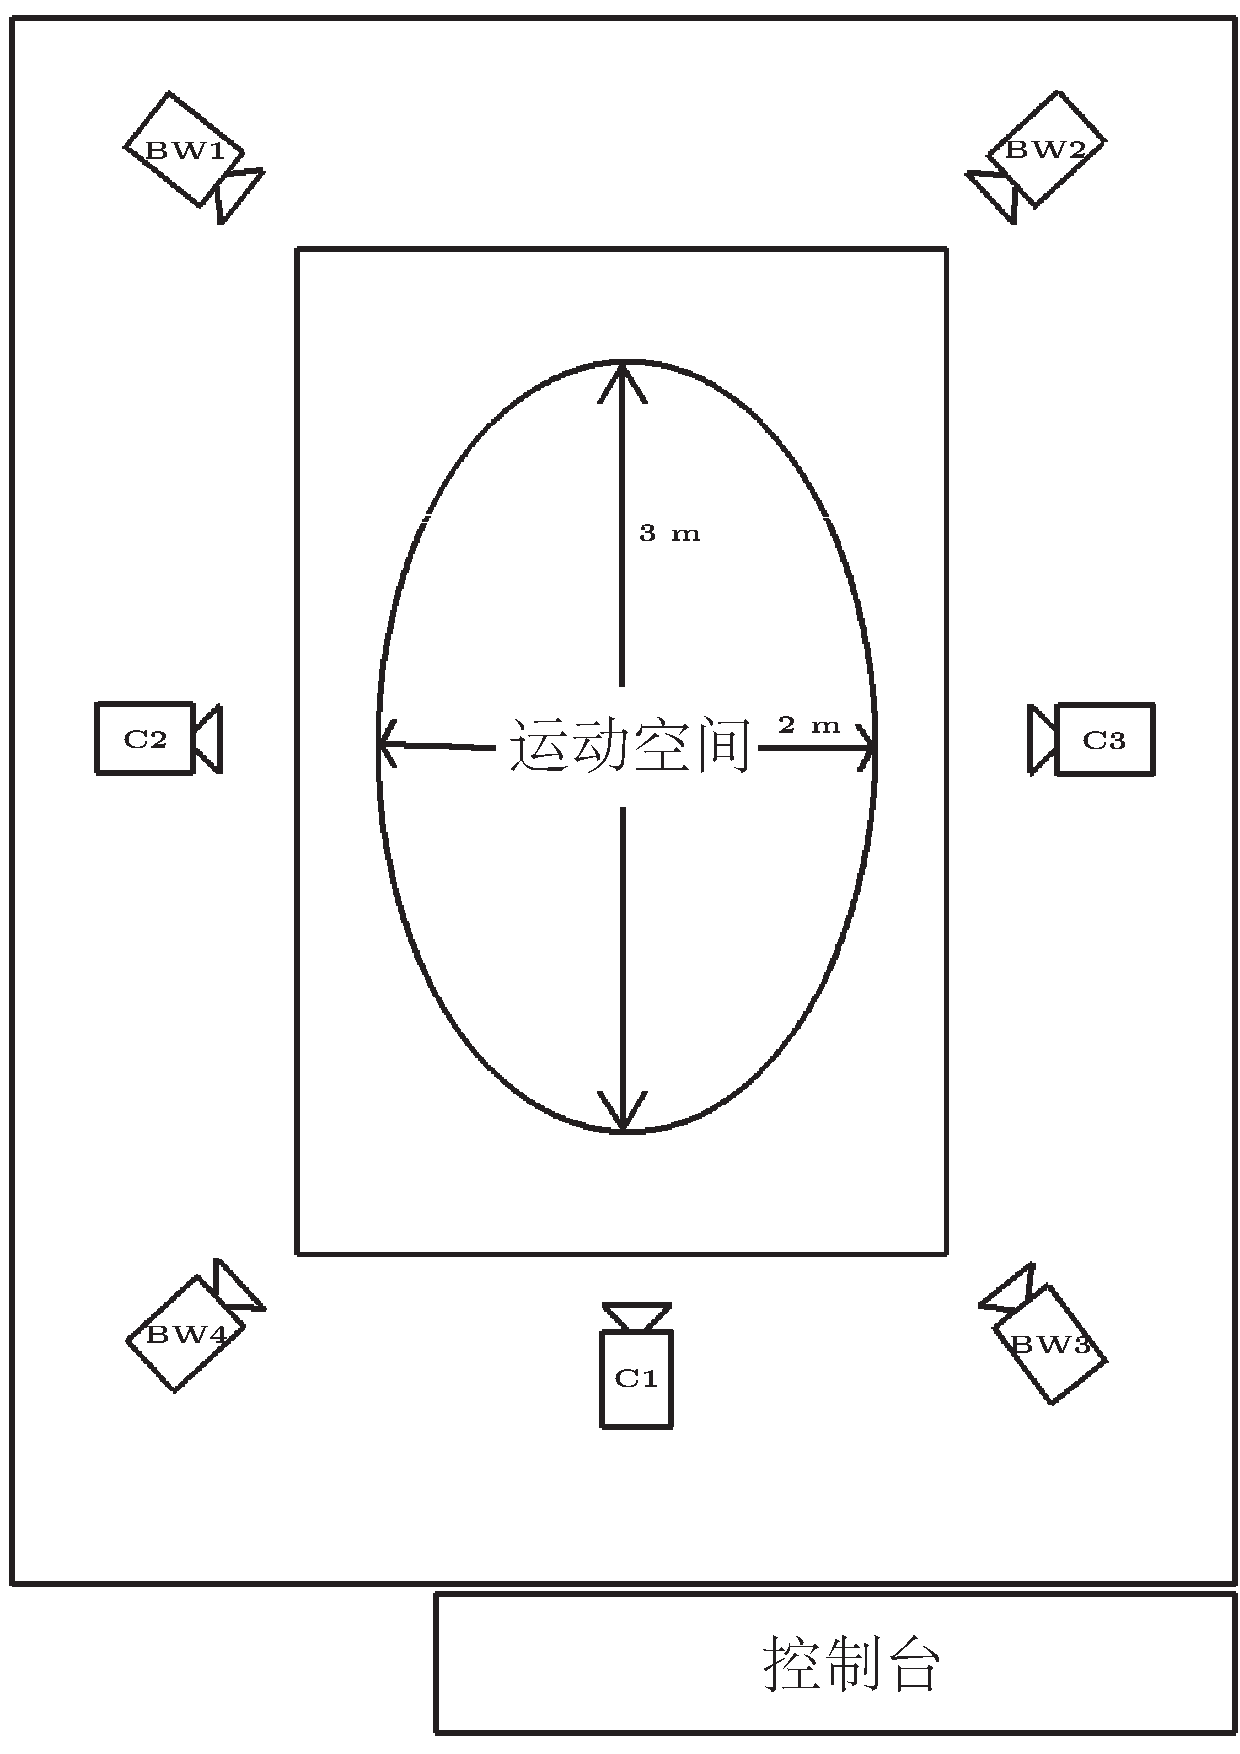
\includegraphics[height=8cm]{camera.pdf}\\
  \caption{相机摆放位置}\label{fig:camera}
\end{figure}

\begin{figure}[htbp]
  \centering
  \subcaptionbox{S1}{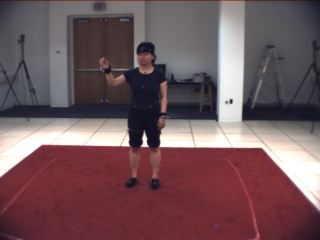
\includegraphics[width=0.4\textwidth]{S1}}\hspace{.5cm}
  \subcaptionbox{S2}{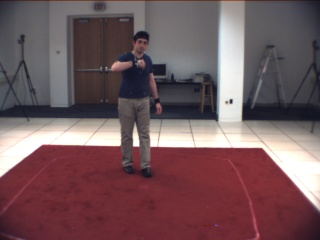
\includegraphics[width=0.4\textwidth]{S2}}\\
  \subcaptionbox{S3}{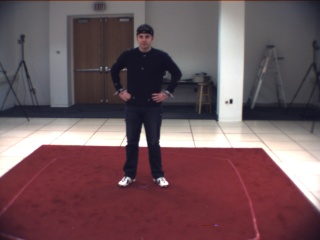
\includegraphics[width=0.4\textwidth]{S3}}\hspace{.5cm}
  \subcaptionbox{S4}{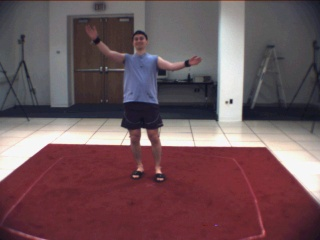
\includegraphics[width=0.4\textwidth]{S4}}
  \caption{HumanEva-I样例}\label{fig:demo}
\end{figure}

然而,数据库只对部分视频资料给出了运动姿态的ground-truth,四号演员的所有视频都只能用来测试,一到三号演员也有一半视频都没有ground-truth。此外,由于运动捕捉系统本身的问题,并不是对所有视频帧都能给出正确的三维姿态,因此经过筛选后\cite{Poppe2007}\cite{bo2010twin}文章所使用的训练数据如表\ref{tab:poppe}所示。在本文中,训练使用的帧数比\cite{Poppe2007}\cite{bo2010twin}文章较多,具体见表\ref{tab:mydataset}。

\begin{table}[htbp]
  \centering
  \caption{\cite{Poppe2007}\cite{bo2010twin}文章所用帧数统计}
  \label{tab:poppe}
    \begin{tabular}{lcccc}
      \toprule[1.5pt]
      动作 & Subject1 & Subject2 & Subject3 & Total \\\midrule[1pt]
      走路 & 1176 & 876 & 895 & 2947 \\
      慢跑 & 439 & 795 & 831 & 2065 \\
      投掷 & 217 & 806 & 0 & 1023\\
      挥手 & 801 & 681 & 214 & 1696\\
      拳击 & 502 & 464 & 933 & 1889\\
      合计 & 3135 & 3622 & 2873 & 9630\\
      \bottomrule[1.5pt]
    \end{tabular}
\end{table}

\begin{table}[htbp]
  \centering
  \caption{本文所用帧数统计}
  \label{tab:mydataset}
    \begin{tabular}{lcccc}
      \toprule[1.5pt]
      动作 & Subject1 & Subject2 & Subject3 & Total \\\midrule[1pt]
      走路 & 1220 & 913 & 976 & 3109 \\
      慢跑 & 506 & 824 & 897 & 2227 \\
      投掷 & 217 & 815 & 0 & 1032\\
      挥手 & 872 & 690 & 260 & 1822\\
      拳击 & 576 & 470 & 996 & 2042\\
      合计 & 3391 & 3712 & 3129 & 10232\\
      \bottomrule[1.5pt]
    \end{tabular}
\end{table}



\section{人体三维骨架表示}
\label{sec:skeleton}

本文采用的人体三维骨架表示方法同\cite{bo2010twin},将人体用20个关节点来描述,每个关节点用$\mathbf{P}=(x,y,z)$三维坐标表示,串联起来构成$20\times3=60$维向量。在二维图像上表示骨架如图\ref{fig:2Ddemo},三维表示如图\ref{fig:3Ddemo},20个关节点的具体含义参见表\ref{tab:20}。为了使每个骨架对齐,我们把躯干远端作为三维坐标的原点,所有其他点坐标都根据原点做平移变换。

\begin{figure}[htbp]
  \centering
  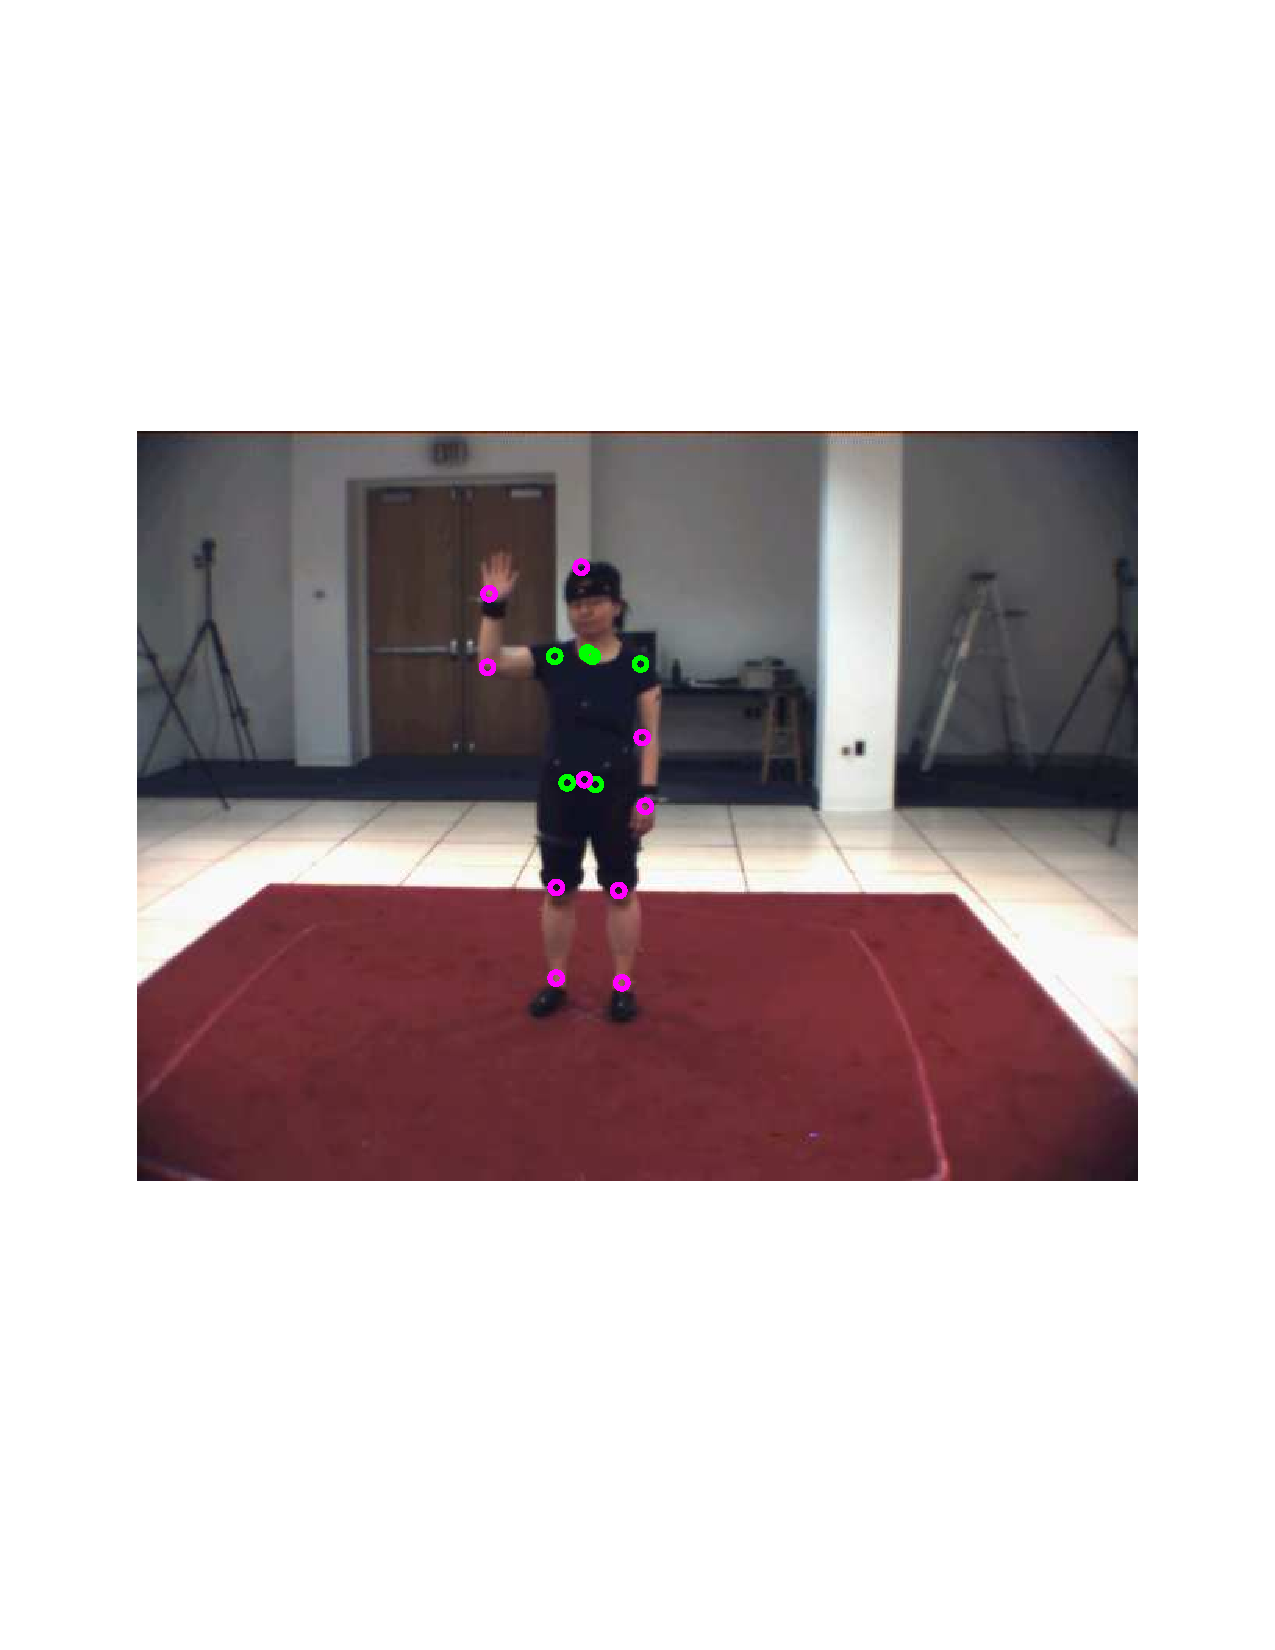
\includegraphics[width=0.7\textwidth]{2Dpose}\\
  \caption{二维骨架表示}\label{fig:2Ddemo}
\end{figure}

\begin{figure}[htbp]
  \centering
  \subcaptionbox{}{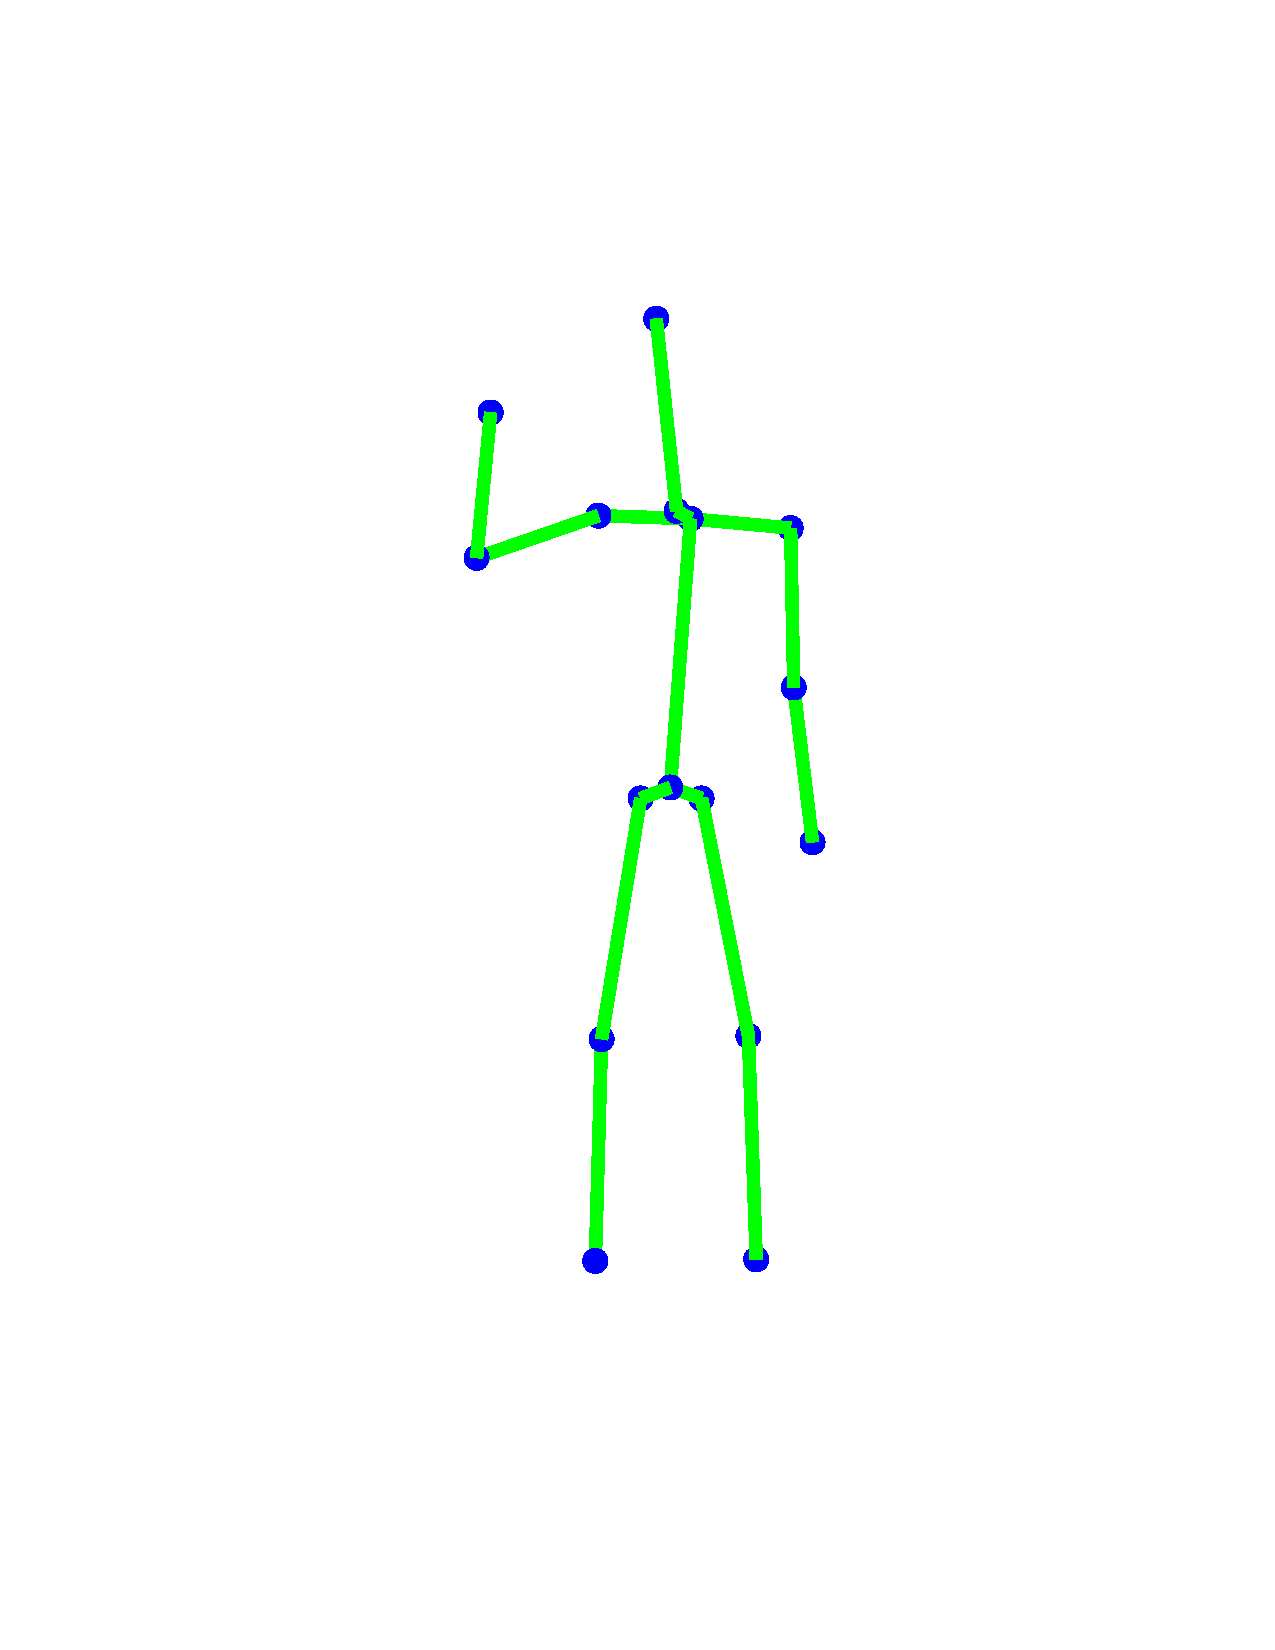
\includegraphics[height=6cm]{3D_1}}\hspace{1cm}
  \subcaptionbox{}{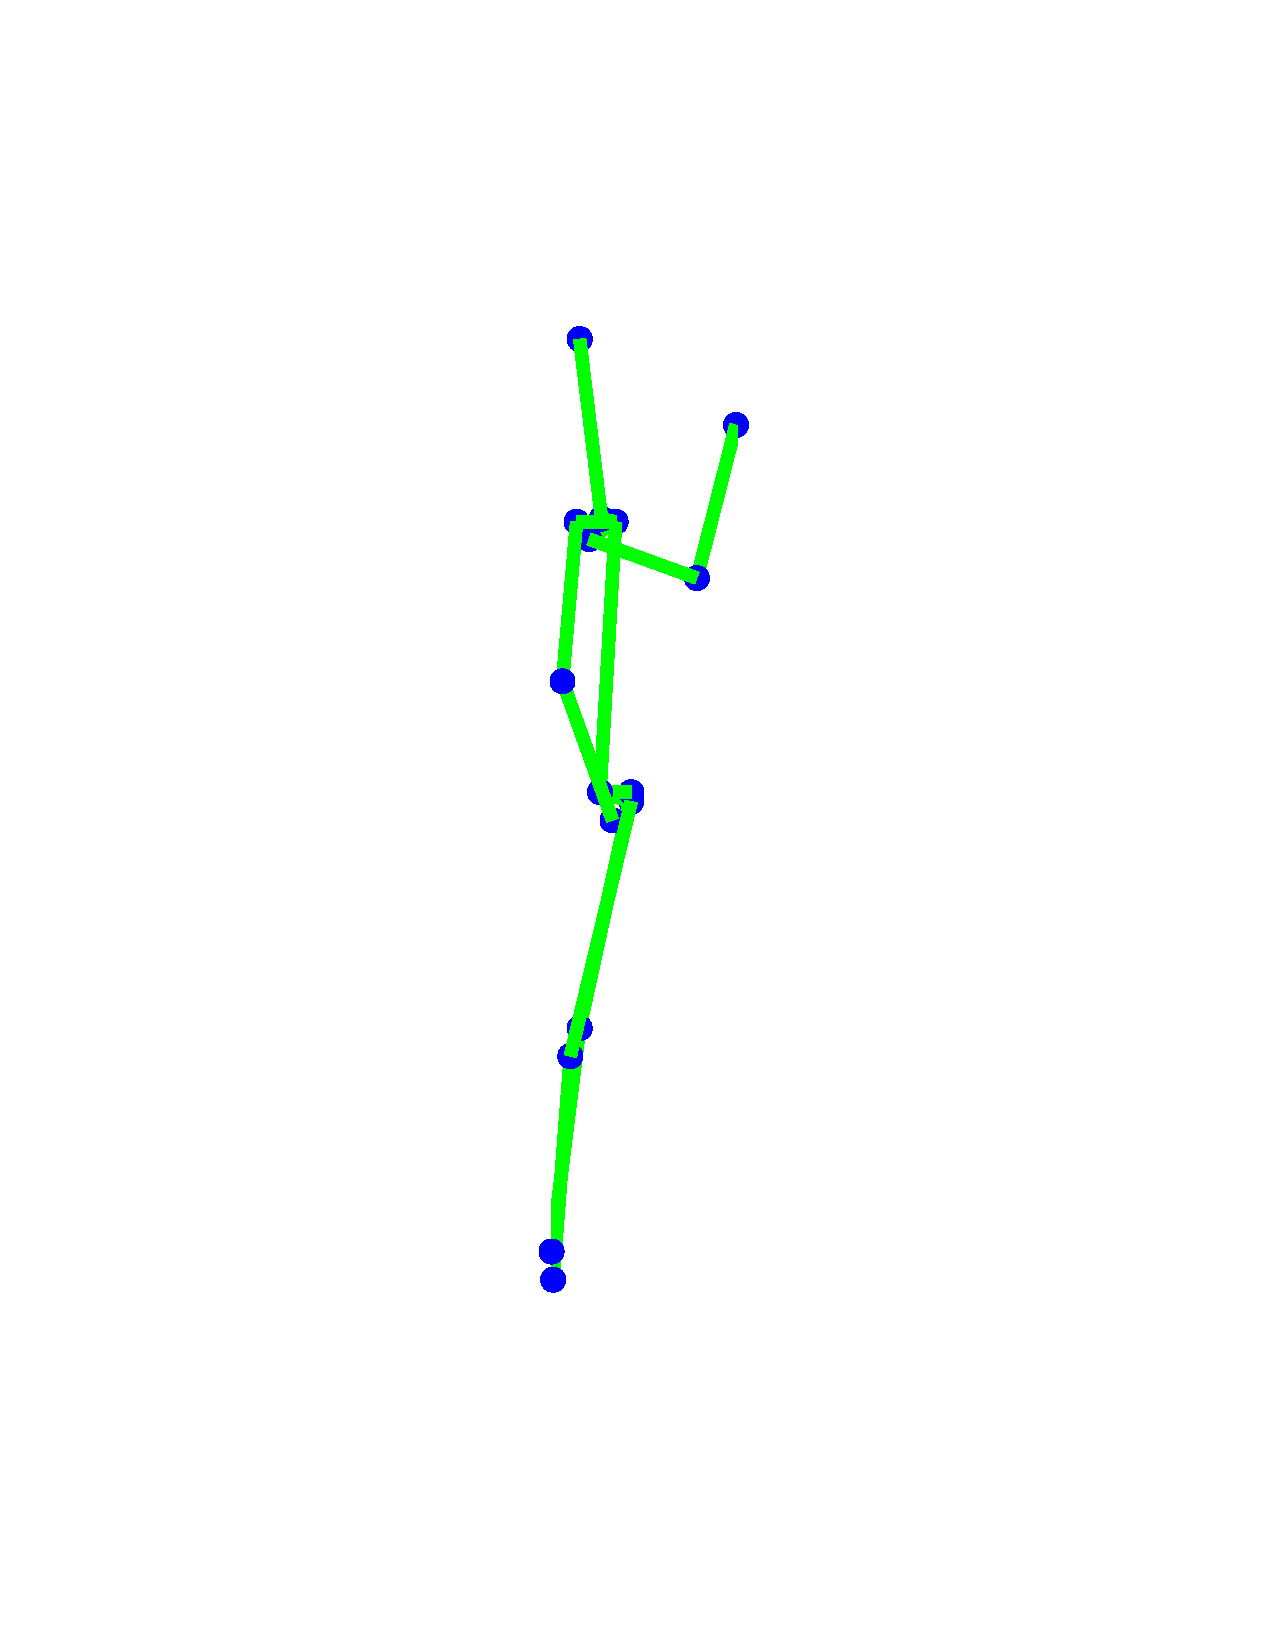
\includegraphics[height=6cm]{3D_2}}\hspace{1cm}
  \subcaptionbox{}{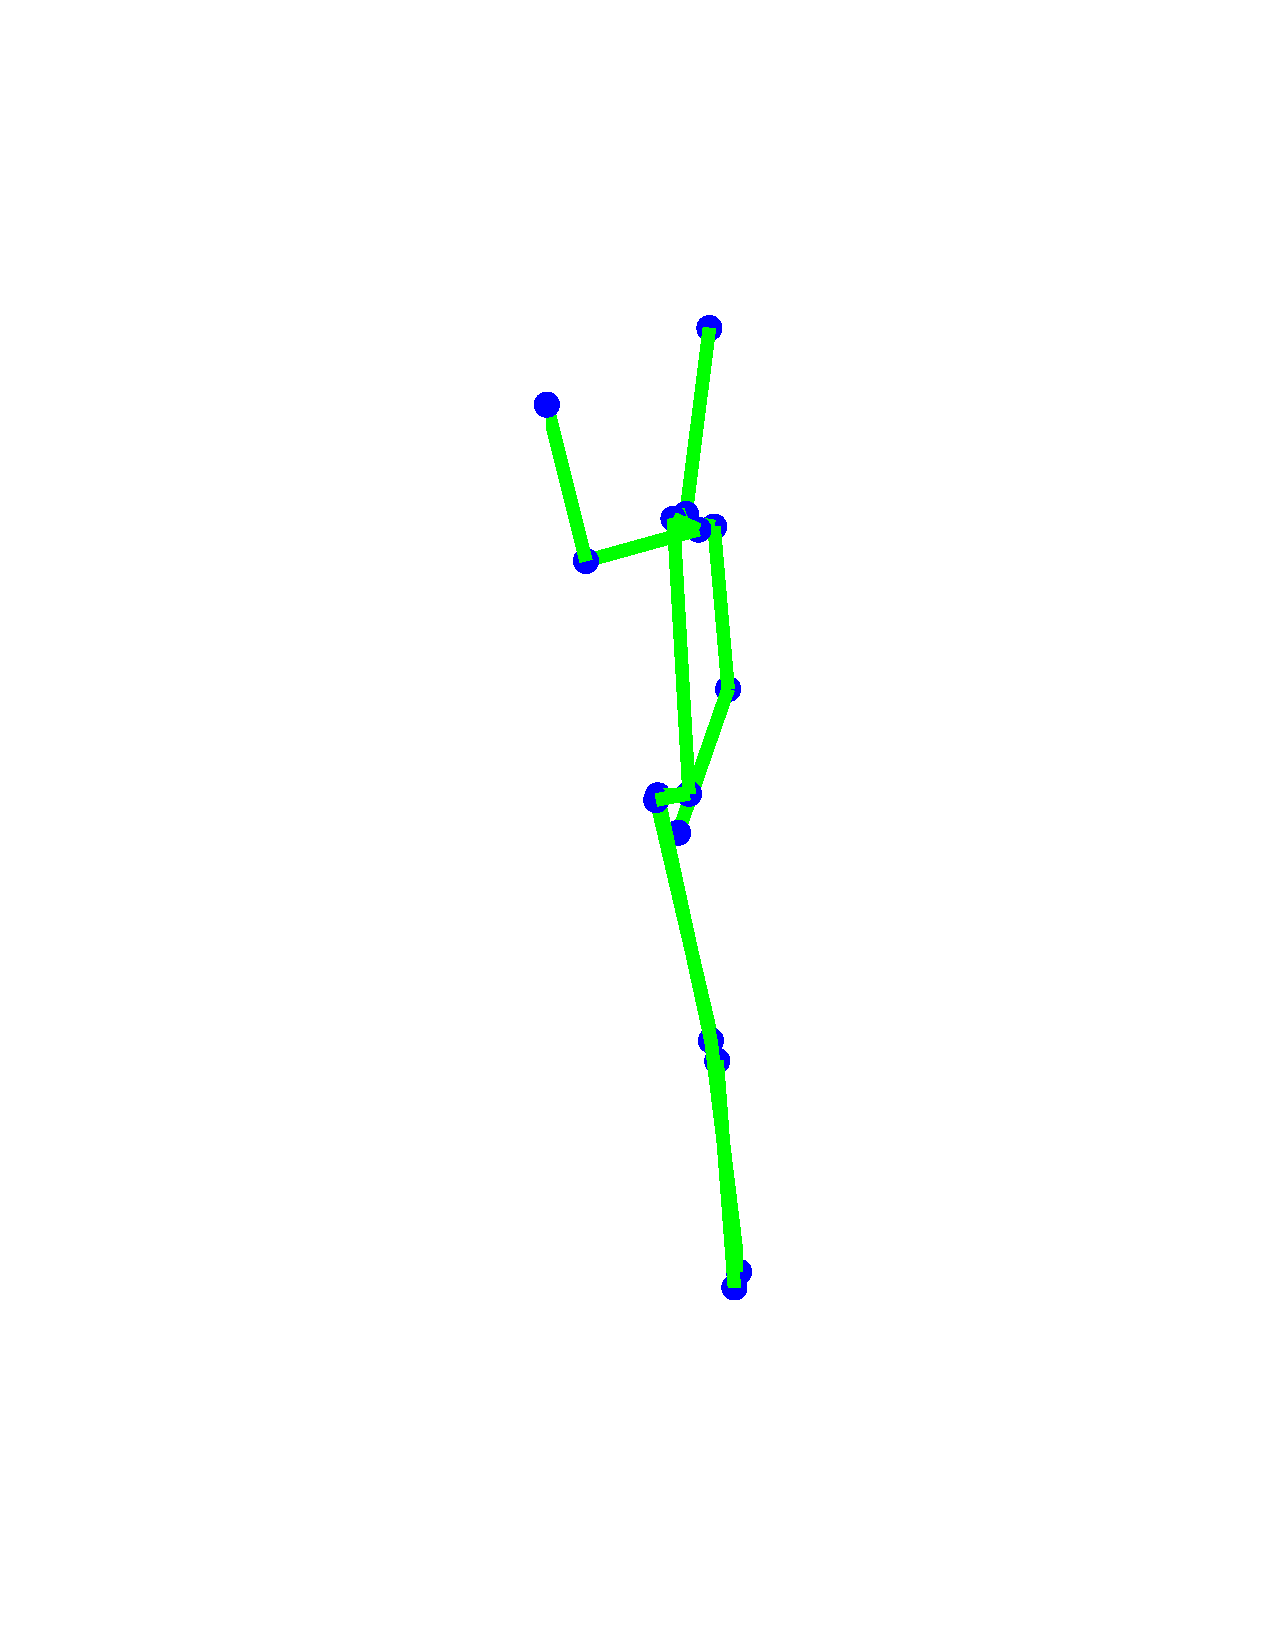
\includegraphics[height=6cm]{3D_3}}
  \caption{三维骨架表示}\label{fig:3Ddemo}
\end{figure}

\begin{table}[htbp]
  \centering
  \begin{tabular}{ccccccccccc}
  \toprule[1.5pt]
    & \multirow{2}{4em}{躯干}  & \multirow{2}{4em}{头部}  & \multicolumn{4}{c}{胳膊} & \multicolumn{4}{c}{腿}\\
    & & & 左前 & 左后 & 右前 & 右后 & 左前 & 左后 & 右前 & 右后 \\\midrule[1pt]
   近端 & 1 & 1 & 1 & 1 & 1 & 1 & 1 & 1 & 1 & 1 \\
   远端 & 1 & 1 & 1 & 1 & 1 & 1 & 1 & 1 & 1 & 1 \\
   \bottomrule[1.5pt]
  \end{tabular}
  \caption{关节点构成}\label{tab:20}
\end{table}

%
%
% %%% 其它部分
% \backmatter
% % 插图索引
% \listoffigures
% % 表格索引
% \listoftables
% % 公式索引
% \listofequations
%
%
% % 参考文献
% \bibliographystyle{thubib}
% \bibliography{ref/refs}
%
%
% % 致谢
% %%% Local Variables:
%%% mode: latex
%%% TeX-master: "../main"
%%% End:

\begin{ack}
  感谢导师戴琼海教授、刘烨斌老师对本人的热情指导,他们帮助我迈出了科研的第一步,做科研的方法将终身受益。
  
  承蒙王雁刚师兄的指导和帮助,我坚定了研究方向,梳理了研究思路,在做不下去的时候,王雁刚师兄一次次给予了我前进的方向和成功的信心。
  
  感谢和我一起讨论问题、交流毕业论文心得的吴蒙蒙、刘金林、胡雪梅等同学,是你们,让毕业设计有了更多的欢声笑语。
  
  最后感谢柯家琪、张洋师兄对我撰写论文给予的帮助,感谢 \thuthesis,它的存在让我的论文写作轻松自在了许多,让我的论文格式规整漂亮了
  许多。
  
\end{ack}

%
% % 附录
% \begin{appendix}
% %%% Local Variables:
%%% mode: latex
%%% TeX-master: "../main"
%%% End:

\chapter{外文资料翻译}
\pagestyle{empty}
%\includepdfset{pagecommand={\thispagestyle{thu@plain}}}
%\includepdf[pages=1-8]{data/FFDB.pdf} %标题
\begin{center}
\sanhao{一种用于视频中表情生成的数据驱动方法}\\
\vspace{10pt}
\wuhao
李凯$^{1,2}$ \text{~~~~} 徐枫$^{1}$ \text{~~~~}王珏$^{3}$ \text{~~~~}戴琼海$^{1}$ \text{~~~~}刘烨斌$^{1}$\\
$^{1}$清华大学自动化系\\
$^{2}$清华大学深圳研究院\text{~~~}
$^{3}$Adobe 系统\\
\end{center}

%摘要
\CJKfamily{hei}\textbf{摘要:}
\CJKfamily{kai}
本文提出了一种方法来用一个人的面部表情视频对目标人脸合成真实的面部动画。不用于以往的面部动画方法,我们的系统利用了现有的目标人物的面部表情数据库,并最终通过从数据库中获取含有与输入相似的表情的帧来生成最终视频。为此我们开发了一种表情相似度度量来准确地测量两个视频帧的表情差异。为了加强时间相干性,我们的系统从相似度度量决定的候选帧中,利用最短路径算法来选择最优的图片。最后,我们的系统采用一种表情映射的方法来进一步减小输入和检索得到的帧之间的表情差异。实验结果显示我们的系统可以利用所提出的数据驱动方法生成高质量面部动画。
%\noindent
%\CJKfamily{hei}\textbf{关键字:}
%\CJKfamily{kai}
%多角度立体视觉,融合,点云,矩阵恢复,压缩感知。

%正文
\CJKfamily{song}
\section{简介}
性能驱动的面部动画在20世纪80年代就已经走红。它指的问题是:将面部表情从一个人映射到另一个,目标是使渲染的目标面部动画和原表情相比真实且一致。

尽管在过去几十年内已经取得了巨大进步,但这个问题依然未解决。之前的方法主要集中于表情的真实度,也就是说,使目标面部的渲染表情主观上接近输入面部的表情。另一方面,逼真的渲染很大程度上被忽视,先前的方法通常使用3D面部模型作为目标头像。目前尚不清楚在给出一个人的表情后,怎样为一个真实人物的面部渲染逼真的动画。此外,许多以前的方法严重依赖诸如在源面部上标记\cite{feature_based, eri},或精细的人机交互做跟踪\cite{performance_driven, drawing}等额外信息。这些方法的应用范围和效率因此比较有限。

在本文中,我们旨在开发一种自动化系统将一个脸部视频的表情转化到另一个人上,从而产生目标人物的自然表情的视频。受到最近在封闭人脸实现~\cite{deng}和人体运动动画~\cite{xufeng}上的数据驱动方法的启发,我们的系统基于现有的目标人物的表情数据库来实现目标。由于数据库提供了目标人脸在不同表情下的自然视频帧,我们可以利用这些做参考来渲染和输入表情匹配的视频。然而,这个任务并不简单,有如下挑战:
\begin{enumerate}[1.]
  \item 怎样测量两个不同人物视频帧的表情相似度;
  \item 怎样高效地搜索数据库以确保生成的视频不仅接近输入表情,也具有时间相干性;
  \item 由于数据库大小有限,不能覆盖所有输入的表情,怎样进一步调整目标视频帧的表情来提高表情准确性。
\end{enumerate}
我们的系统采用一套技术来解决这些挑战。具体来说,我们提出一个新颖的测量视频中不同人物表情的相似度。为了在时间相干性和表情匹配精度上平衡,我们先从数据库找到K近邻作为每个输入帧的候选,用优化方法来求得最优输出序列。最后,考虑到每个输入和检索帧的细微表情差异,我们提出一种表情转移方法,用这个结果来进一步细化获得的帧的表情。实验结果显示我们的系统能合成时间上连贯且与输入匹配的逼真的面部表情动画。
\section{相关工作}
这项工作与以前在面部表情匹配、面部表情重定向(映射)、视频到视频合成方面研究工作相关。
\subsection{面部表情匹配}
我们的要求是找到最相似的苗青,而不是把面部运动分类到具体、事先定义的类别。在表情识别社区中使用的特征,比如Gabor小波~\cite{Gabor}, LBP~\cite{lbp}和FACS~\cite{facs},或许能提供一种替代方法。然而,他们经常没能考虑身份的差异。比如,一个有胡子的笑脸与没有胡子的笑脸,就LBP特征而言是不同的。只有拥有足够的有胡子和没胡子的训练样本,分类器才能辨别两个笑脸是一样的。此外,这些度量也许不能推断出一个连续的实值距离测量,这意味着他们经常不足以精确地捕捉细微的表情差异。比如CERT~\cite{CERT},仅仅能较好识别峰值表情的活动单元。还不清楚它分辨细微的AU运动能有多好。相反,这两个主要问题在我们提出的表情相似度测量中不存在。

\subsection{3D基于模型的面部表情重定位}
在表情建模和重定位方面已有大量工作。在基于PCA的模型中,比如AAM~\cite{AAM}\\ /CLM~\cite{Saragih},3D形变模型~\cite{morphable},多线性模型~\cite{multilinear,replacement},和变形模型~\cite{face_off},通用基础通过保留主成分从大训练数据中学习来。他们以丢失精细的细节为代价努力换取鲁棒地跟踪所有表情。然而在我们的精炼方法中,在两个相似表情的图片中光流可以更好地捕捉细节表情的不同,从而获得更精确地重定位结果。有特殊特征的形状融合模型为实时动画而建立~\cite{realtime_kinect}。然而,形状融合变形器的数量是模型覆盖度和很总适应性之间的矛盾。其他系统~\cite{photographs,cloning,reanimating} 努力建立纹理逼真的3D面部模型。然而,获得完全纹理p的3D模型并不容易。

\subsection{基于图片的表情映射}
一些人脸合成系统直接在2D图片上操作来实现表情转移。Williams的系统~\cite{performance_driven}从源和目标图片提取面部特征,用特征差异引导扭曲。Liu等人~\cite{eri} 提出 Expression Ratio Image (ERI)通过捕捉光照变化来加强表情映射。Zhang\emph{ et al.}~\cite{geometry_driven}用几何元通过融合样例脸部图片来计算每个图片子区域的纹理。然而,这些方法通常不能处理两幅图片间大的拓扑变化。我们的方法通过从拥有和输入相似的表情的数据库中获得目标脸部克服了这个局限。此外,这些方法通常是劳动密集型的。

\subsection{视频到视频的合成}
我们的工作涉及到之前视频到视频合成系统。和我们的目标相似,Kemelmacher-Shlizerman等人~\cite{eccv10}利用数据库,在一个人联视频驱动下合成一个目标人物的面部视频。然而,他们的系统主要着眼于测量面部表情的相似度。最终视频只是简单地由独立的最相似的图片连接合成,这可能时间上不一致。视频面部替代系统~\cite{replacement} 在保证时空一致性的基础上用源视频的面部代替目标视频中的人脸。然而,它假设输入和目标视频之间粗糙的语义对应和大致相近。

\section{系统概览}
\renewcommand{\figurename}{图}
\begin{figure}[htbp]
\centering
    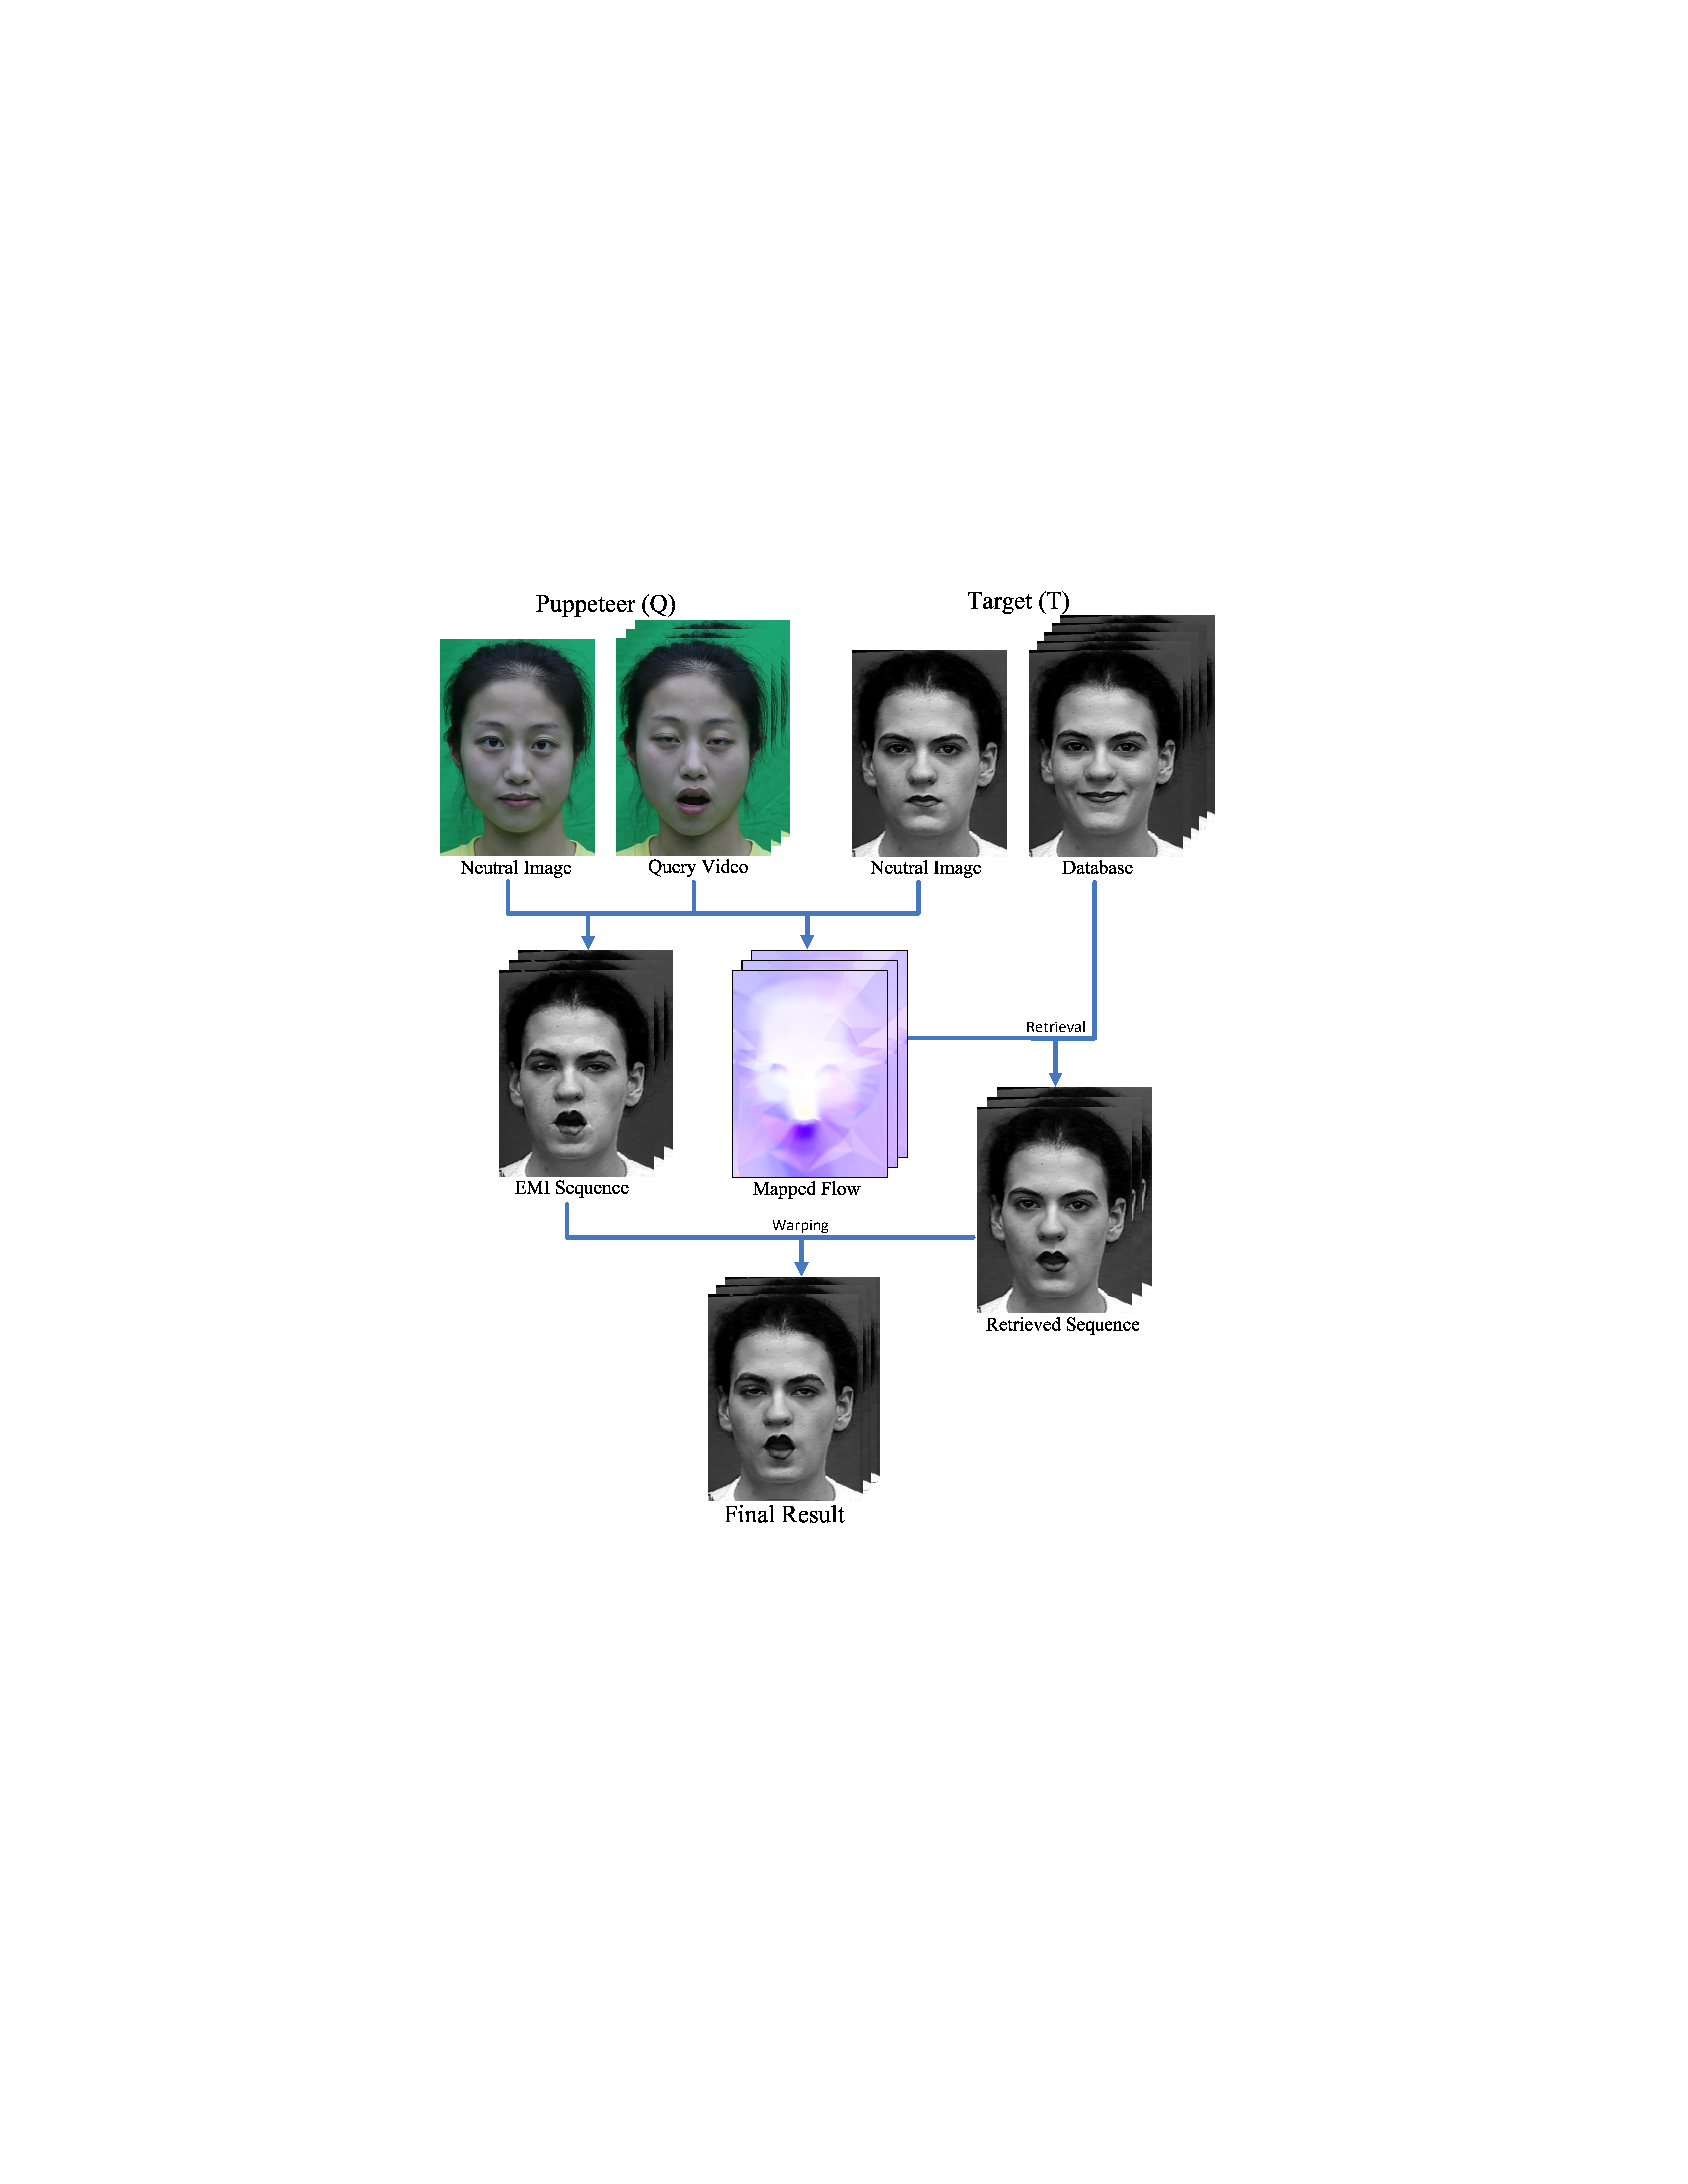
\includegraphics[width=0.95\textwidth]{data/img/overview.pdf}
    \caption{系统概览. 首先将每个查询帧和它的中性面部之间的光溜映射到目标人,用来从数据库中检索。同时,目标人的中性图像被扭曲以生成含有查询表情的EMI序列。最后,检索序列用EMI 精炼,来生成最终结果。}
    \label{fig:overview}
\end{figure}
图~\ref{fig:overview}展示了我们系统的概况。要为目标人生成逼真的表情,我们首先捕捉一段这个人展示基本表情的视频,比如生气、恐惧、惊奇、伤心、高兴、厌恶。有了另一个我们叫做人偶师(puppeteer)的人的面部表情,我们的方法尝试利用目标人的数据合成同样的表情。

具体而言,对于每个输入帧,我们使用第~\ref{sec:metric}章描述的基于光流相似度度量方法查询数据库获得$k$个与输入帧有最相近表情的目标人的视频帧。正如在第~\ref{sec:retrieval} 章描述的那样,我们把这个任务认为是和最短路问题一样找最优连续帧,而不是像Kemelmacher-Shlizerman等人~\cite{eccv10} 直接用最相似的帧生成一个匹配序列。获得的序列包含和人偶师相似且时间一致的表情。

然而,由于数据库大小有限,为每个输入帧找到一个完美的表情匹配几乎是不可能的,更何况,一些表情的人偶师具有独特的特点。为了考虑再输入和检索帧之间细微的表情差异,我们用一个表情映射技术来生成另一个候选面部,我们称之为EMI图像,如第~\ref{sec:emi}章描述那样。EMI图片通常有比检索帧有更精确的面部表情,但她的面部外观可能有重大瑕疵。在最后一步,我们把EMI图片和检索帧结合起来从而生成有精确表情和逼真外观的最终输出帧,如第~\ref{sec:emi}章所述。
\section{算法}
\subsection{表情相似度度量}\label{sec:metric}
给出人偶师的面部图片$Q_e$, 我们的系统试图从目标人的数据库中找到对应面部图片$T_e$,这幅图片有和$Q_e$最接近的面部表情. 为此我们需要能准确测量$Q_e$ 和 $T_e$之间表情差异的面部相似度度量, 同时忽视两幅图片的外表差异。

为了找到这样一个度量,我们的系统使用人偶师和目标人的中性面,分别记作$Q_n$ 和 $T_n$。当我们建立数据库的时候 $T_n$ 只需要标识一次,我们假设 $Q_n$ 在输入视频中由用户标记。为了说明人偶师的面部如何从 $Q_n$ 到 $Q_e$变化,我们能计算两幅图片中的光流场~\cite{celiu}记作 \mbox{\boldmath $F$}$_{Q_n \to Q_e}\in\mathbb{R}^{m \times 2}$, 这里$m$表示$Q_n$中的所有人脸像素。为了从光场中去除全局头部运动,我们用不随表情变化的鼻子区域来估计2D相似度变化,在计算表情差异前先把$Q_e$和$Q_n$对齐。我们也用脸的宽度归一化光流。类似的,$T_n$和$T_e$之间的光流场\mbox{\boldmath $F$}$_{T_n \to T_e}\in\mathbb{R}^{n \times 2}$, 其中$n \neq m$, 也可以计算。然而,由于身份/外观不同我们不能直接对比这两个光场。
\begin{figure}[htbp]
\centering
    \subcaptionbox{面部标记}{
    \label{fig:face_marker}
    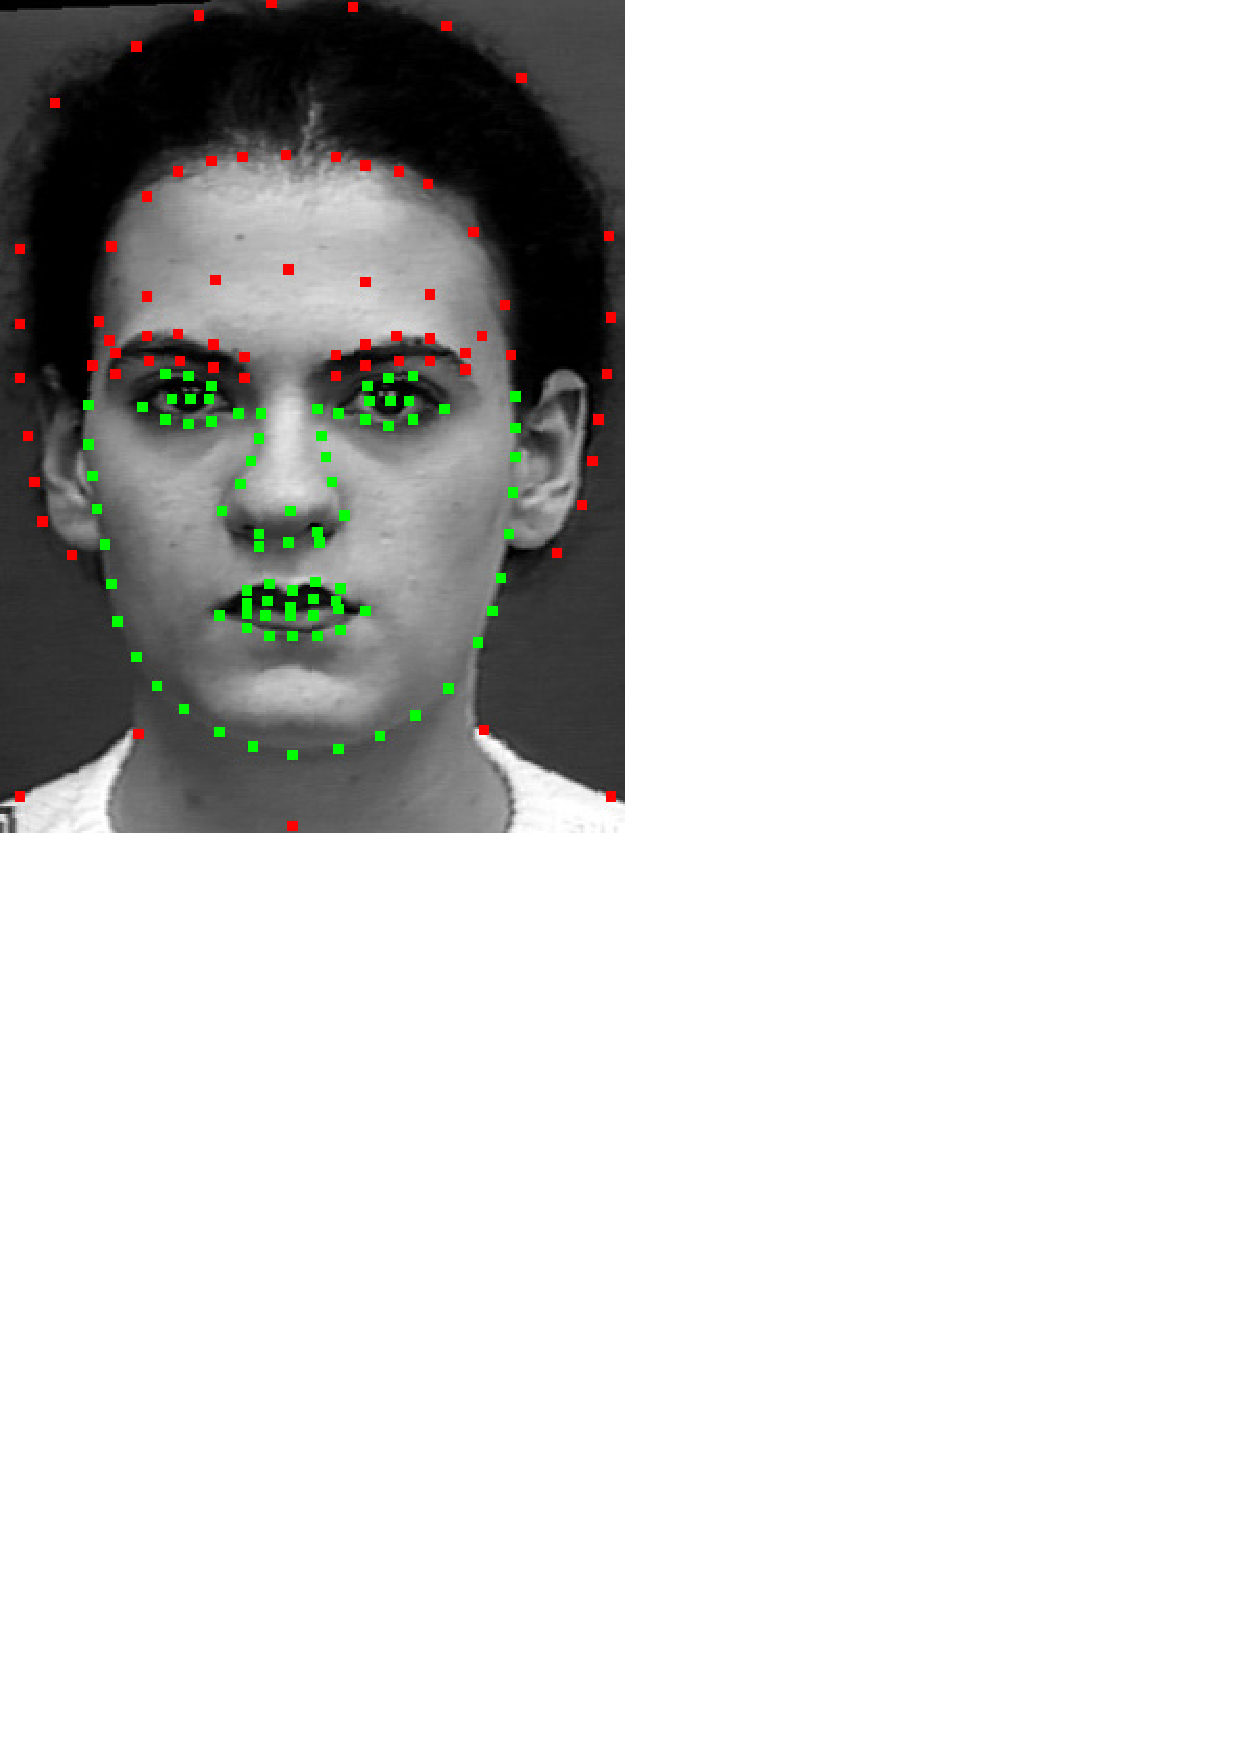
\includegraphics[width=0.20\textwidth]{data/img/facemarker.pdf}}
    \hspace{5mm}
    \subcaptionbox{局部区域}{
    \label{fig:face_region}
    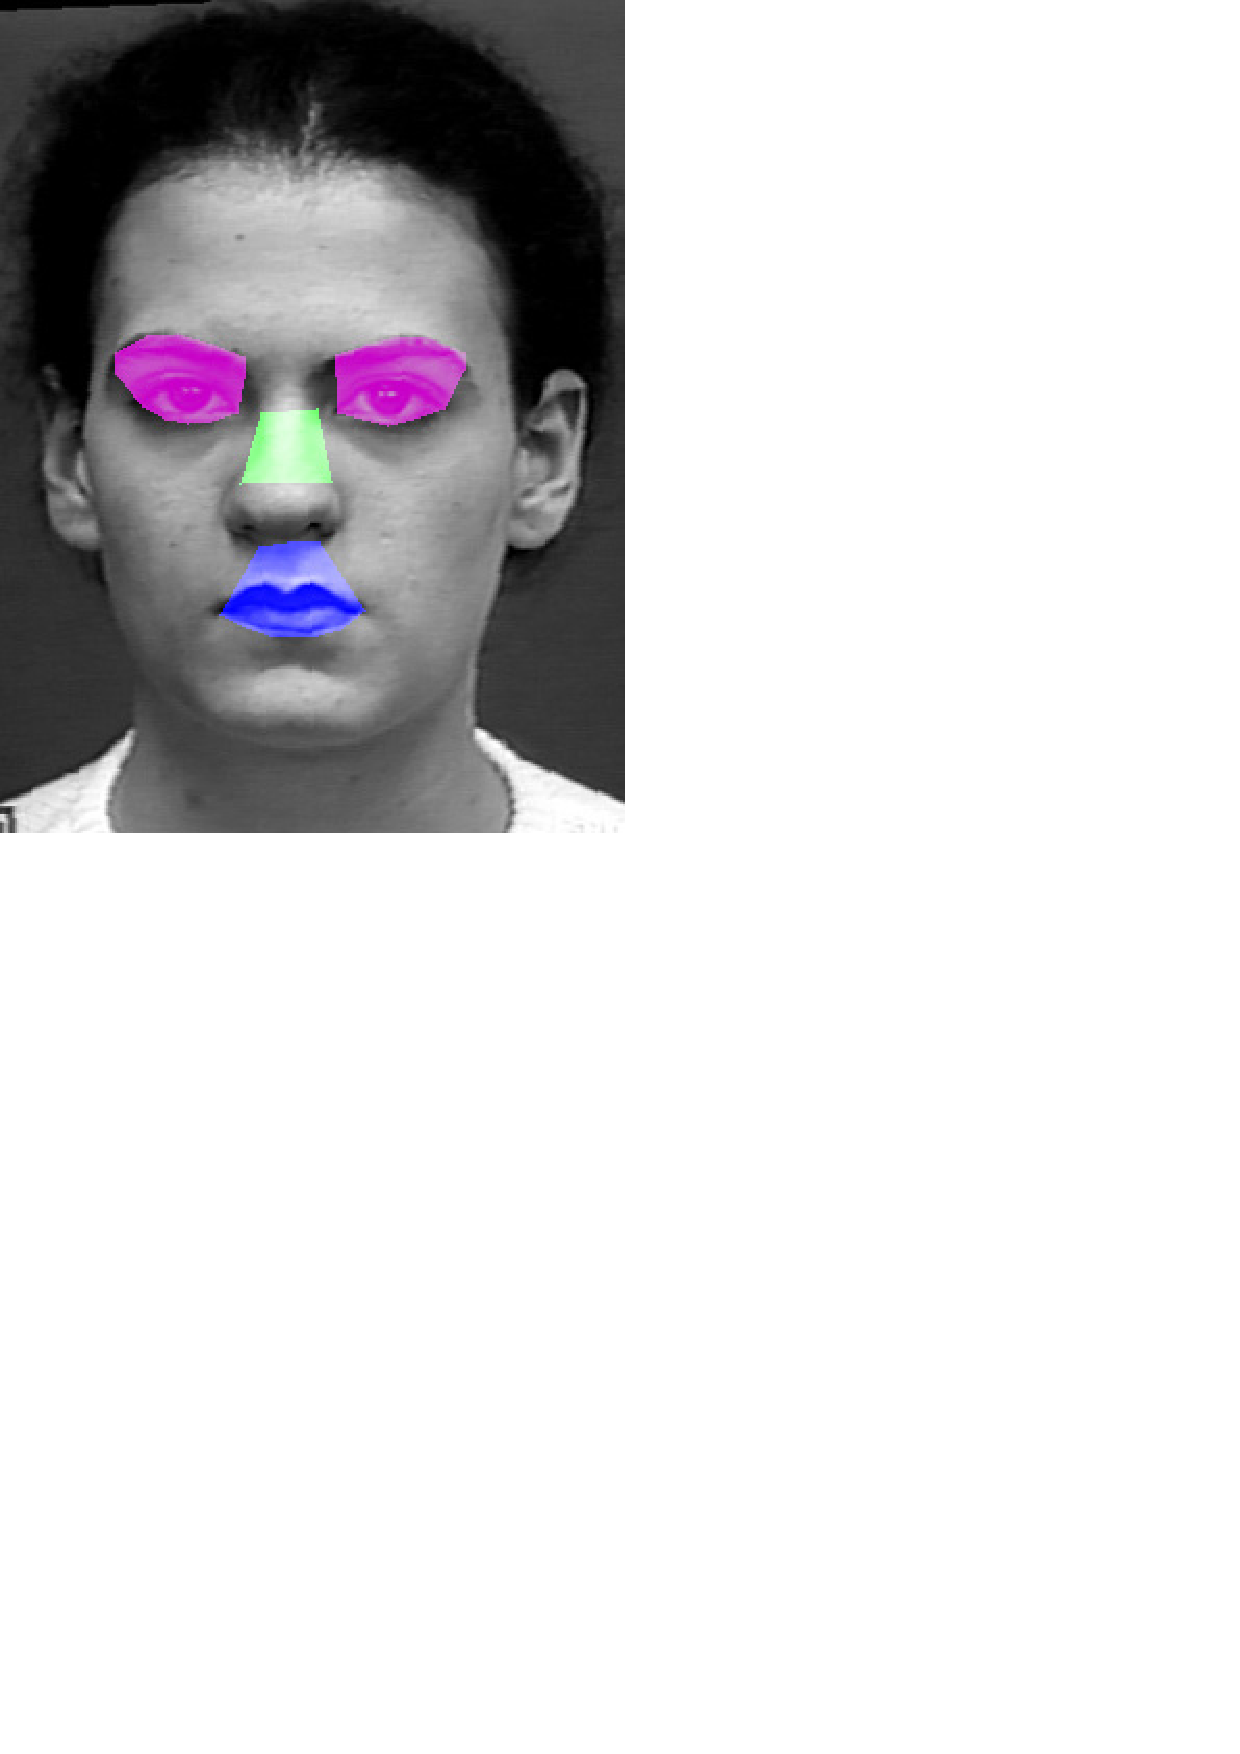
\includegraphics[width=0.20\textwidth]{data/img/faceregion.pdf}}
    \caption{中性脸初始化 (a) 绿色是ASM的标记,红色是手工标记
    (b) 眼睛、嘴巴、鼻子区域分别用品红、蓝色、绿色标记。}
    \label{fig:face}
\end{figure}
为了在两个光场之间建立精确的对应,我们首先使用Active Shape Model (ASM)~\cite{asm}只检测在中性面$Q_n$和$T_n$的面部标志物,该方法对于中性表情的正面人脸很有效。然而它无法覆盖我们算法在之后几步中需要的所有面部。因此我们在两个中性面上手工标注标志点,如图~\ref{fig:face_marker}所示。然后我们用Delauney三角网标出$Q_n$ 和 $T_n$ 中的脸部区域,这引出一个只能像素注册函数$g: Q_n \to T_n$。此外,由于两个身份之间的语义对应应该对不同的面部表情具有不变性,可以合理假设$g': Q_e \to T_e$两个表情图片的注册函数近似和$g: Q_n \to T_n$ 相同。有了注册函数,对于一个点$\vec{a}\in Q_n$转移到$\vec{a}' \in Q_e$,它在$T_n$对应的光流向量按如下计算:
\begin{equation}\label{eq:map2}
\Delta \vec{b}=g(\vec{a}')-g(\vec{a}),
\end{equation}
其中$\vec{b}=g(\vec{a})$是$T_n$上$\vec{a}$的对应点。

通过在$Q_n$上的所有面部像素应用这个映射,我们获取了一种映射好的光流场\mbox{\boldmath $F$}$'_{Q_n \to Q_e}$,可以通过与\mbox{\boldmath $F$}$'_{Q_n \to Q_e}$对比测量两个表情有多接近。以往工作指出~\cite{eccv10},表情差异的主要来源是眼睛和嘴巴区域,因此我们只用这些区域的像素来计算表情相似度(参见图~\ref{fig:face_region})。直接的方法是通过绝对的光流差计算$Q_e$ 和 $T_e$之间的表情差异:
\setlength\arraycolsep{1pt}
\begin{eqnarray}\label{eq:dist_mag}
d_e(Q_e, T_e)&=& \alpha_{e}\sum_{i\in\text{eye}}\left\|F'_{Q_n \to Q_e,i} -F_{T_n \to T_e,i}\right\| \nonumber\\
  &&+\alpha_{m}\sum_{i\in\text{mouth}}\left\|F'_{Q_n \to Q_e, i} -F_{T_n \to T_e, i}\right\|,
\end{eqnarray}

这里下标$i$表示光流矩阵\mbox{\boldmath $F$}中第$i$行。$\alpha_{\{e, m\}}$分别是眼睛和嘴巴区域的权重。
\begin{figure}[htbp]
\centering
    \subcaptionbox{}{
    \label{fig:metric_driven}
    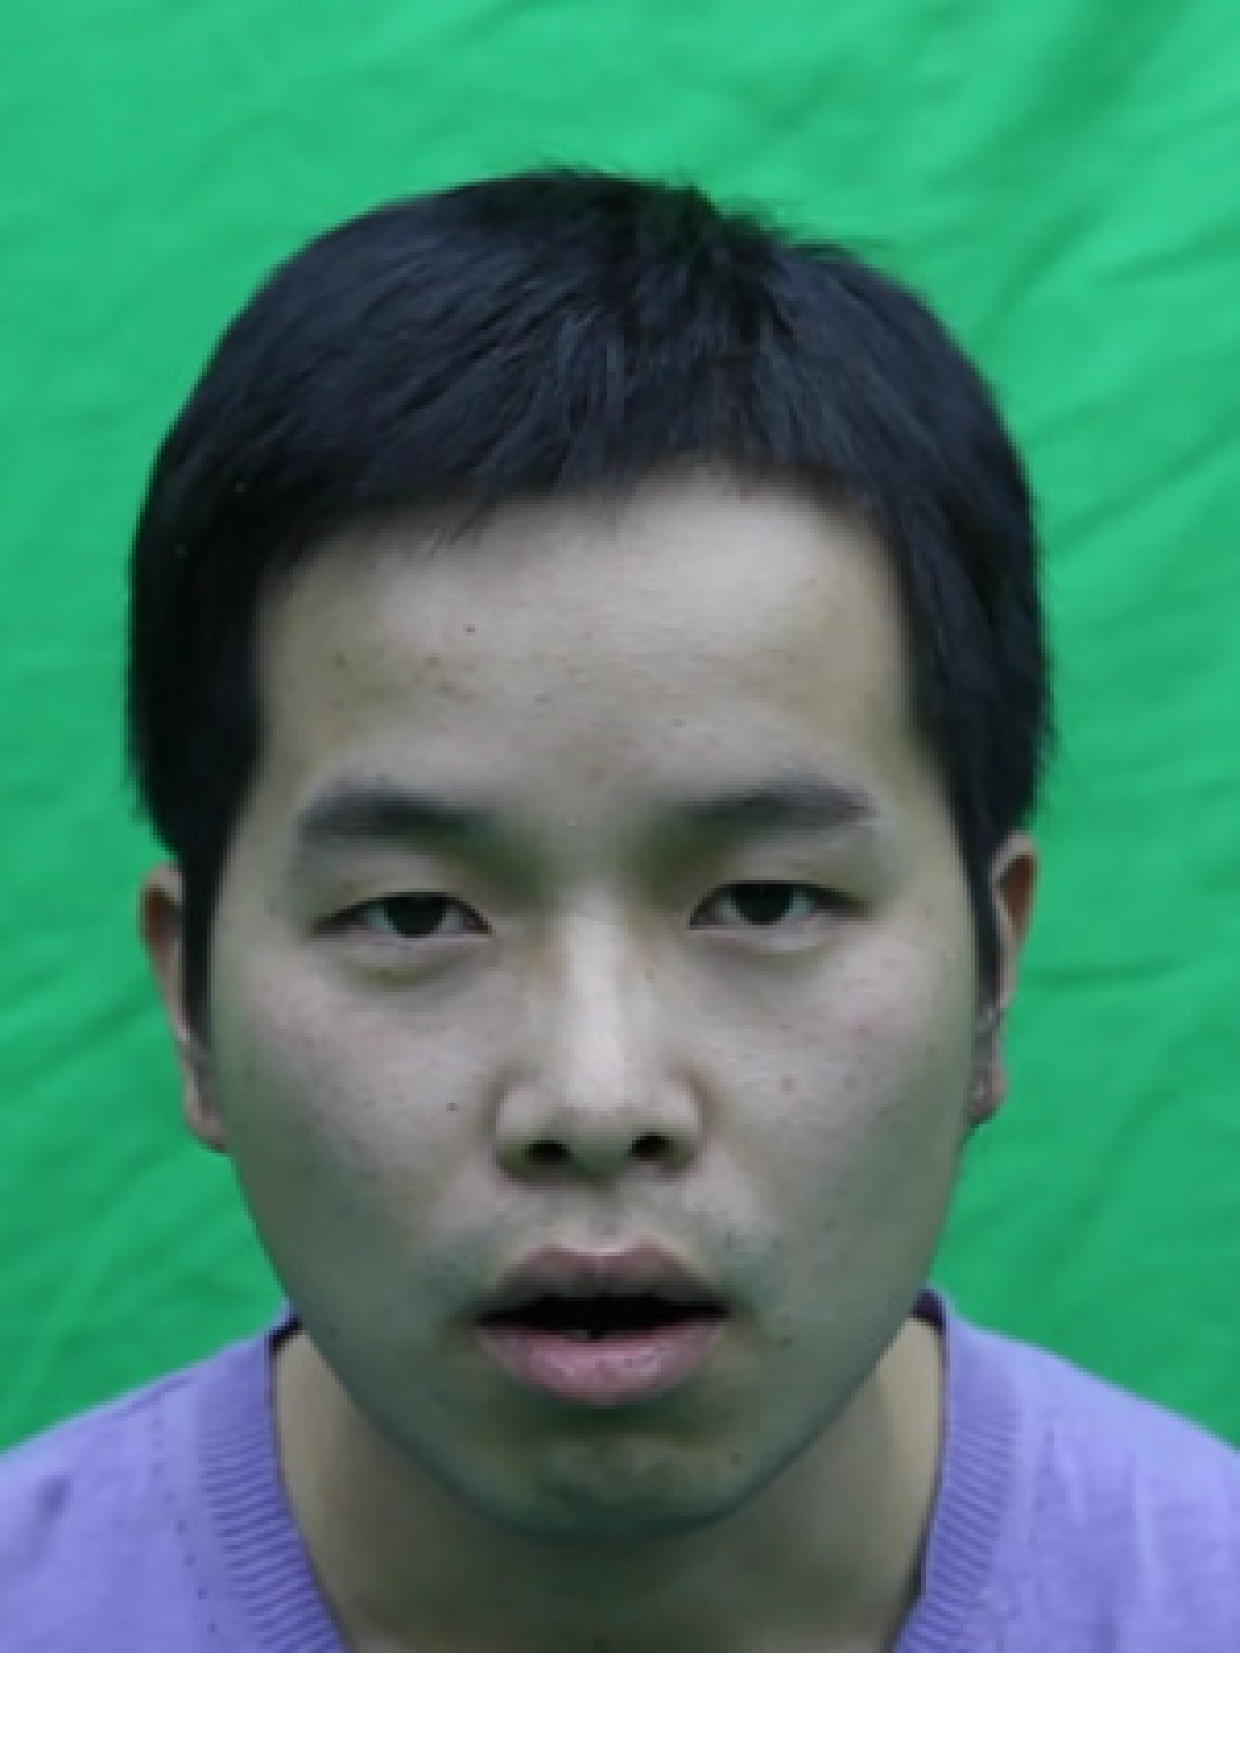
\includegraphics[width=0.2\textwidth]{data/img/metric_likai_0380_00103.pdf}}
    \subcaptionbox{}{
    \label{fig:metric_lbp}
    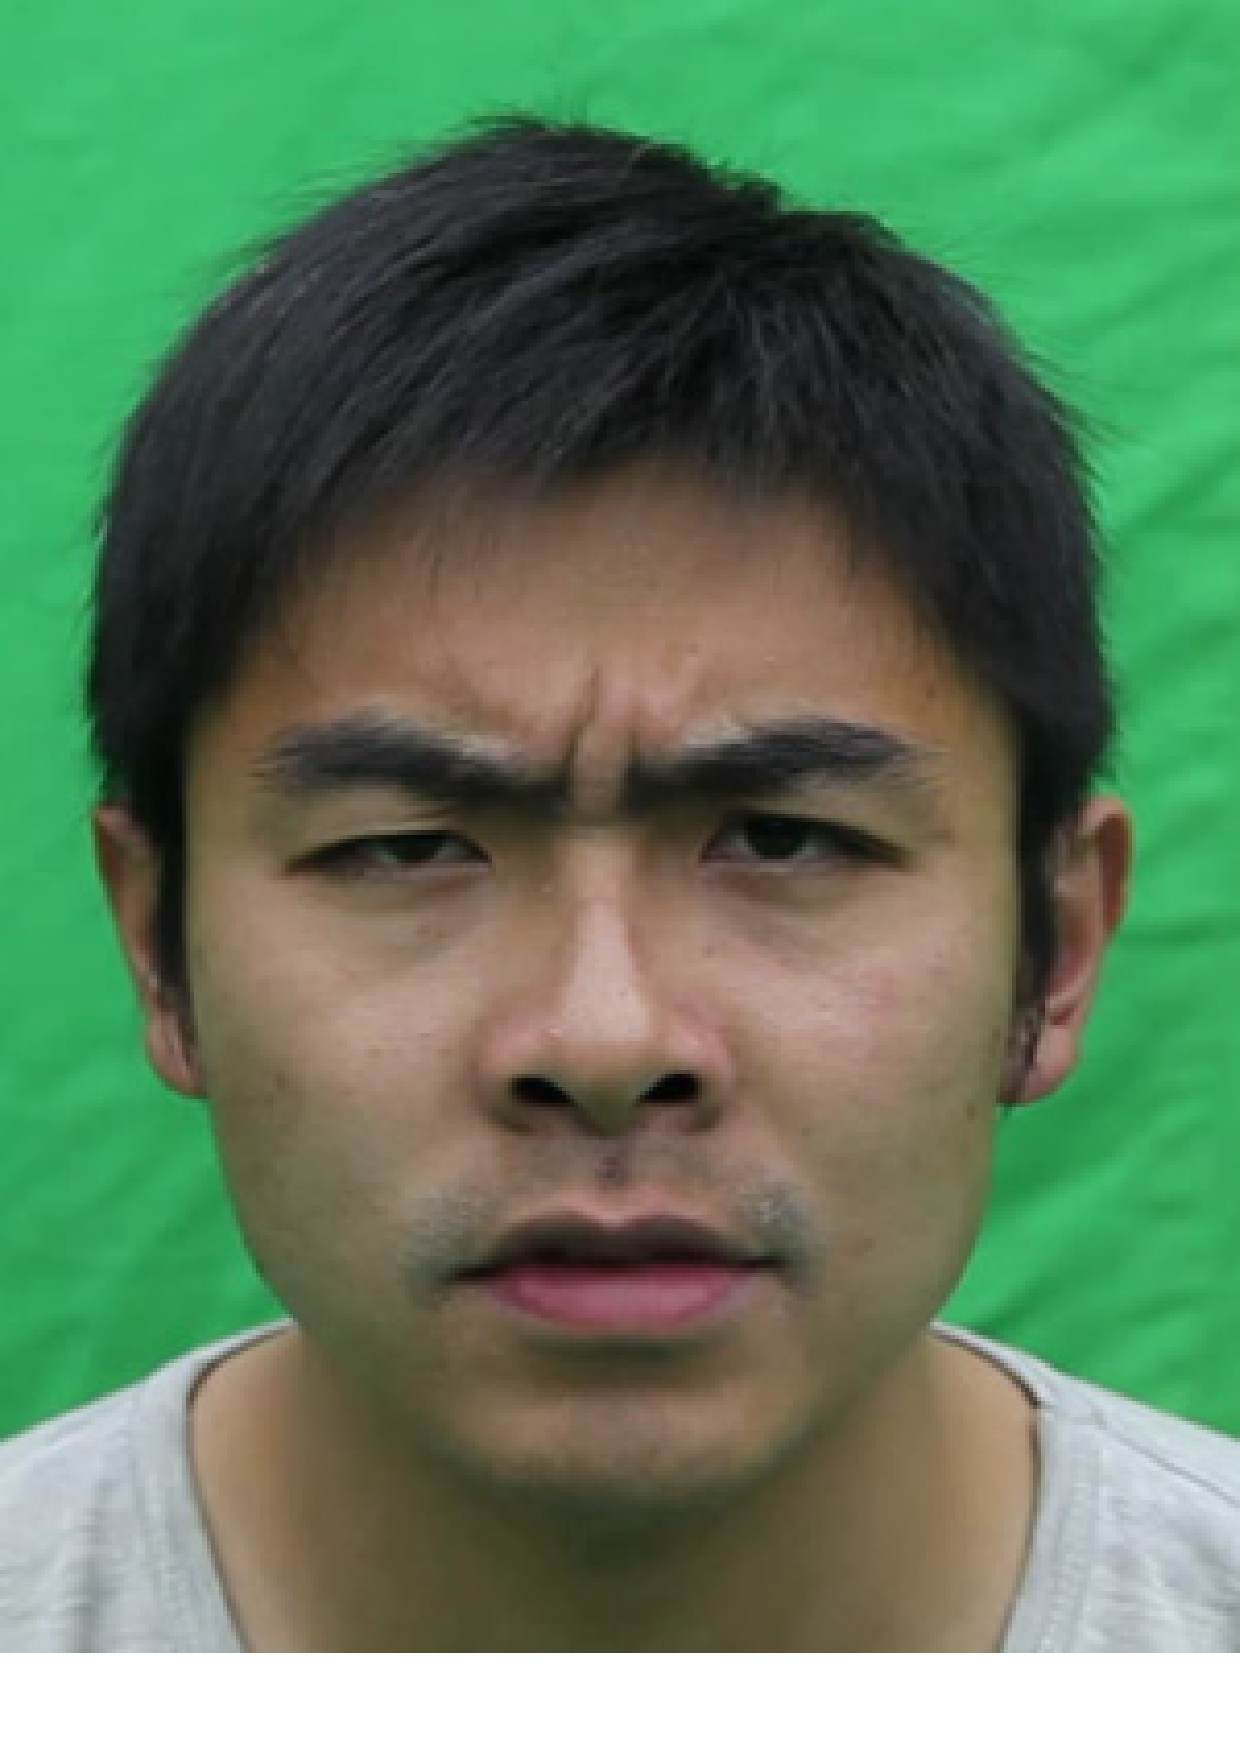
\includegraphics[width=0.2\textwidth]{data/img/metric_lbp_00102.pdf}}
    \subcaptionbox{}{
    \label{fig:metric_mag}
    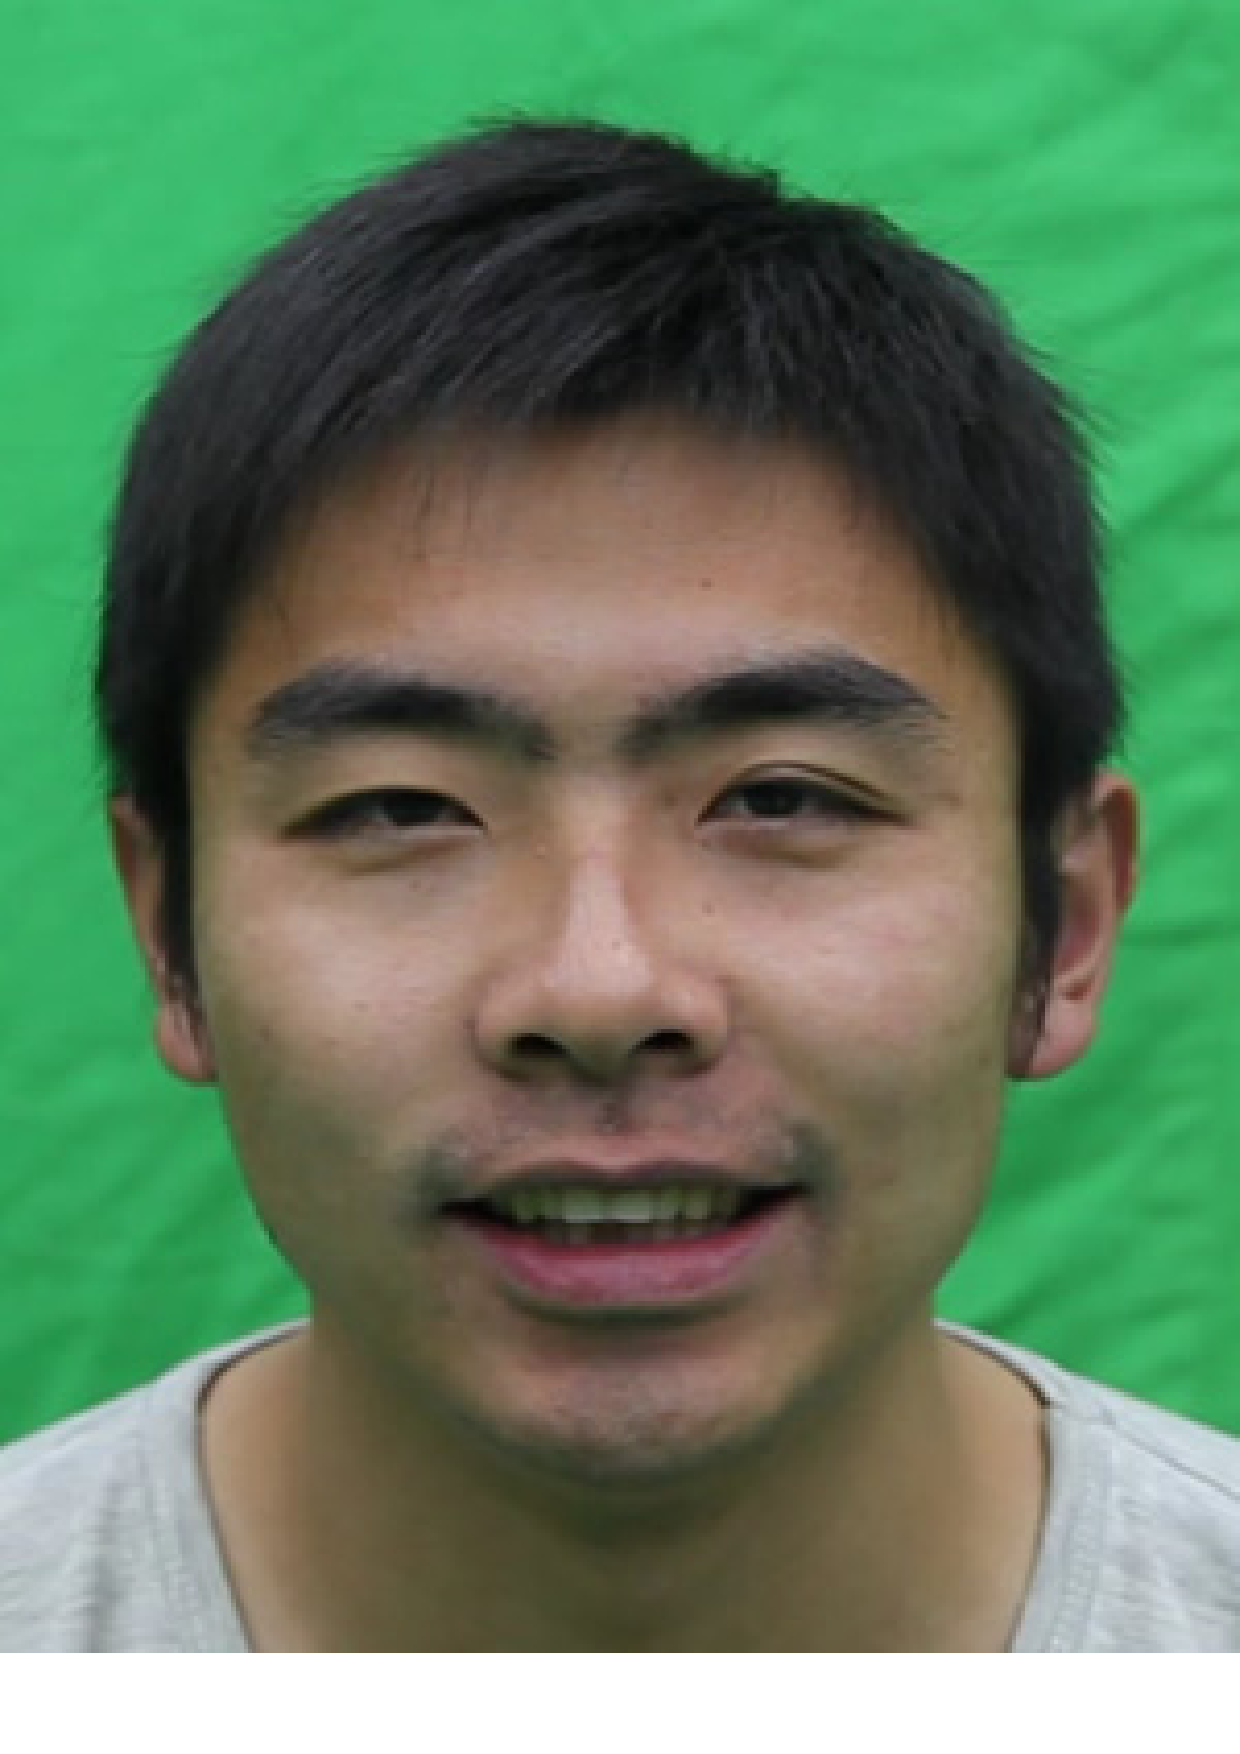
\includegraphics[width=0.2\textwidth]{data/img/metric_OFmag_00102.pdf}}
    \subcaptionbox{}{
    \label{fig:metric_magori}
    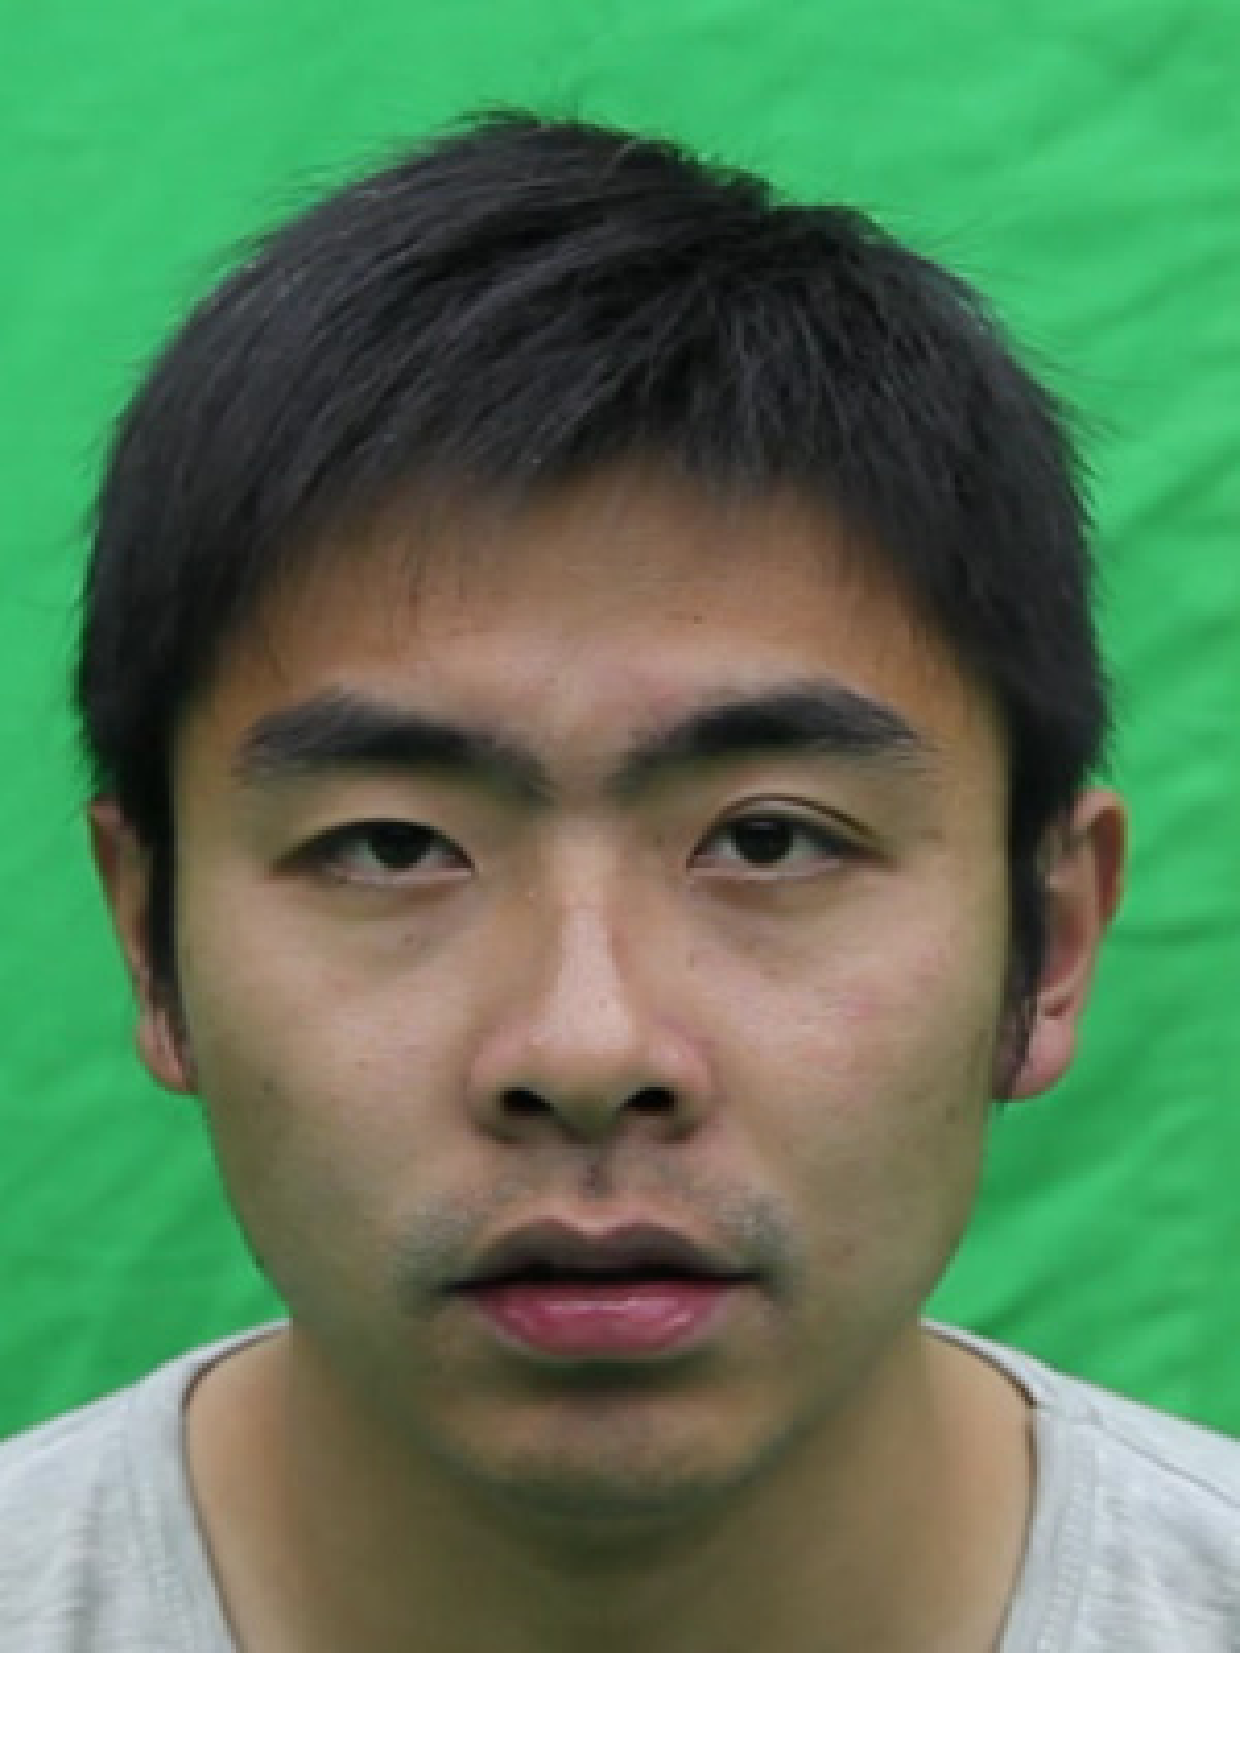
\includegraphics[width=0.2\textwidth]{data/img/metric_OFmagori_00102.pdf}}
    \caption{表情度量对比。 (a) 查询帧。 (b) 由LBP方法得到的最相似表情,它有一个不理想的皱眉。 (c) 由等式~\ref{eq:dist_mag}获得的最相似表情,有一个笑容而不是惊奇。 (d) 由等式~\ref{eq:dist_comb}获得的最相似表情,和查询帧匹配很好}
    \label{fig:metric}
\end{figure}

等式~\ref{eq:dist_mag}中的距离度量在我们大多数实验中都很成功,但我们发现会偶尔产生如图~\ref{fig:metric}所示的错误。这是因为在等式~\ref{eq:dist_mag}中,我们仅考虑了\mbox{\boldmath $F$}$'_{Q_n \to Q_e}-$\mbox{\boldmath $F$}$_{T_n \to T_e}$的光流差异的大小。但光流的方向通常包含更多有关表情的重要信息。比如笑脸通常与嘴角的上翘相关,而哭脸和嘴角下弯相关。这表明在$Q_e$中的表情与$T_e$中的很不一样,如果\mbox{\boldmath $F$}$'_{Q_n \to Q_e}$到\mbox{\boldmath $F$}$_{T_n \to T_e}$的差异方向很不一样,即便差异大小很小。有了这个发现,我们重新设计表情距离度量如下:
\setlength\arraycolsep{1pt}
\begin{eqnarray}
d_b(\vec{u},\vec{v})&=&\beta_m|\vec{u}-\vec{v}|+\beta_o(-\vec{u}\cdot\vec{v}+|\vec{u}||\vec{v}|), \label{eq:d0}\\
d_e(Q_e, T_e)&=&\alpha_{e}\sum_{i\in\text{eye}}d_b(F'_{Q_n \to Q_e,i}, F_{T_n \to T_e,i})\nonumber\\
           &&+\alpha_{m}\sum_{i\in\text{mouth}}d_b(F'_{Q_n \to Q_e, i}, F_{T_n \to T_e, i}),\label{eq:dist_comb}
\end{eqnarray}

这里$\beta_{\{m, o\}}\in[0,1]$分别是大小和方向的权重,且$\beta_m+\beta_o=1$。 当$\beta_o$ 等于零,等式~\ref{eq:dist_comb}简化为等式~\ref{eq:dist_mag}。在等式~\ref{eq:d0} 中的偏移量$|\vec{u}||\vec{v}|$确保方向项非负。注意此距离度量不保证对称性和三角不等式。为使之更有数学味,可以计算反向距离$d_e(T_e,Q_e)$,用二者平均值作为最终距离度量。但实际上我们发现这并无必要,因为$d_e(Q_e, T_e)$已很好描述不同身份两张图片的表情差异,对我们的应用而言已足够。
\subsection{基于检索的视频合成}\label{sec:retrieval}
使用如上定义的相似性度量,一个视频合成的简单方法是为每个输入帧,找到其在数据库中的最近邻表清,并叠在一起,以形成最终的输出视频。然而,我们发现这种方法并不很好,在最终视频中面部表情的时间相干性没有得到很好的保持,并且最终的视频经常出现抖动。补充材料包含了说明此问题的视频。我们的系统采用了一些额外的技术来解决的时间一致性问题,我们将在本小节详细介绍。
\subsubsection{结合表情速度}
首先,在公式~\ref{eq:dist_comb}中定义的距离度量只考虑了两个面部的表情相似度。然而在视频中,我们需要关心在每一帧表情变化的速度。最相似的帧应该是表情及其变化速度都与查询帧相符的。为了保证表情速度,我们在视频序列中简单地计算另一个在当前帧和下一帧之间的光流。记$Q_e^{(q)}$为第 $q$个查询帧,表情速度计算如下:
\begin{equation}\label{eq:dF_Q}
\text{d} \mbox{\boldmath $F$}_{Q_e^{(q)}} = \mbox{\boldmath $F$}_{Q_e^{(q)}\to Q_e^{(q+1)}}.
\end{equation}

类似的,对于在数据库中的帧$T_e^{(t)}$,我们计算表情速度为d\mbox{\boldmath $F$}$_{T_e^{(t)}}$。同样,由于$Q_e^{(q)}$ 和 $T_e^{(t)}$身份和表情差异,直接计算d\mbox{\boldmath $F$}$_{Q_e^{(q)}}$ 和 d\mbox{\boldmath $F$}$_{T_e^{(t)}}$ 距离并不好。需要扭曲表情速度光流场来去除身份差异,如我们在
第~\ref{sec:metric}章所做。我们还需要扭曲两者的速度光流场来把他们映射到中性表情,以去除他们的表情差异。

具体说,对于数据库帧,我们把\mbox{\boldmath $F$}$_{T_n\to T_e^{(t)}}$的反向光流用于 d\mbox{\boldmath $F$}$_{T_e^{(t)}}$,导出与中性表情$T_n$相符的扭曲的表情速度流d\mbox{\boldmath $F$}$'_{T_e^{(t)}}$。对于查询帧$Q_e^{(q)}$,我们把公式~\ref{eq:dist_comb} 计算的反向光流\mbox{\boldmath $F$}$'_{Q_n\to Q_e^{(q)}}$用于d\mbox{\boldmath $F$}$_{Q_e^{(q)}}$,导出与中性表情$T_n$相符的扭曲的表情速度流d\mbox{\boldmath $F$}$'_{Q_e^{(q)}}$。最后,$Q_e^{(q)}$ 和 $T_e^{(t)}$的表情速度差异计算如下:
\begin{eqnarray}\label{eq:dist_deri}
d_v(Q_e^{(q)}, T_e^{(t)})&=& \alpha_{e}\sum_{i\in\text{eye}}d_b(\text{d}F'_{Q_e^{(q)}, i}, \text{d}F'_{T_e^{(t)}, i})\nonumber\\
           &&+\alpha_{m}\sum_{i\in\text{mouth}}d_b(\text{d}F'_{Q_e^{(q)}, i}, \text{d}F'_{T_e^{(t)}, i}),
\end{eqnarray}

此处函数$d_b(\cdot,\cdot)$在公式~\ref{eq:d0}中定义。结合公式~\ref{eq:dist_comb}和公式\ref{eq:dist_deri},最终的视频表情距离度量定义如下:
\begin{equation}\label{eq:dist_all}
\mathcal{D}(Q_e^{(q)}, T_e^{(t)})=\gamma_e d_e(Q_e^{(q)}, T_e^{(t)})+ \gamma_v d_v(Q_e^{(q)}, T_e^{(t)}),
\end{equation}

这里$\gamma_{\{e,v\}}\in[0,1]$分别是表情距离和表情速度距离的权重,满足$\gamma_e+\gamma_v=1$。

图~\ref{fig:velocity}的例子表明,当表情很微妙,在度量中结合表情速度能帮助系统更好的捕捉表情变化。
\begin{figure}[htbp]
\centering
    \subcaptionbox{}{
    \label{fig:velocity_driven}
    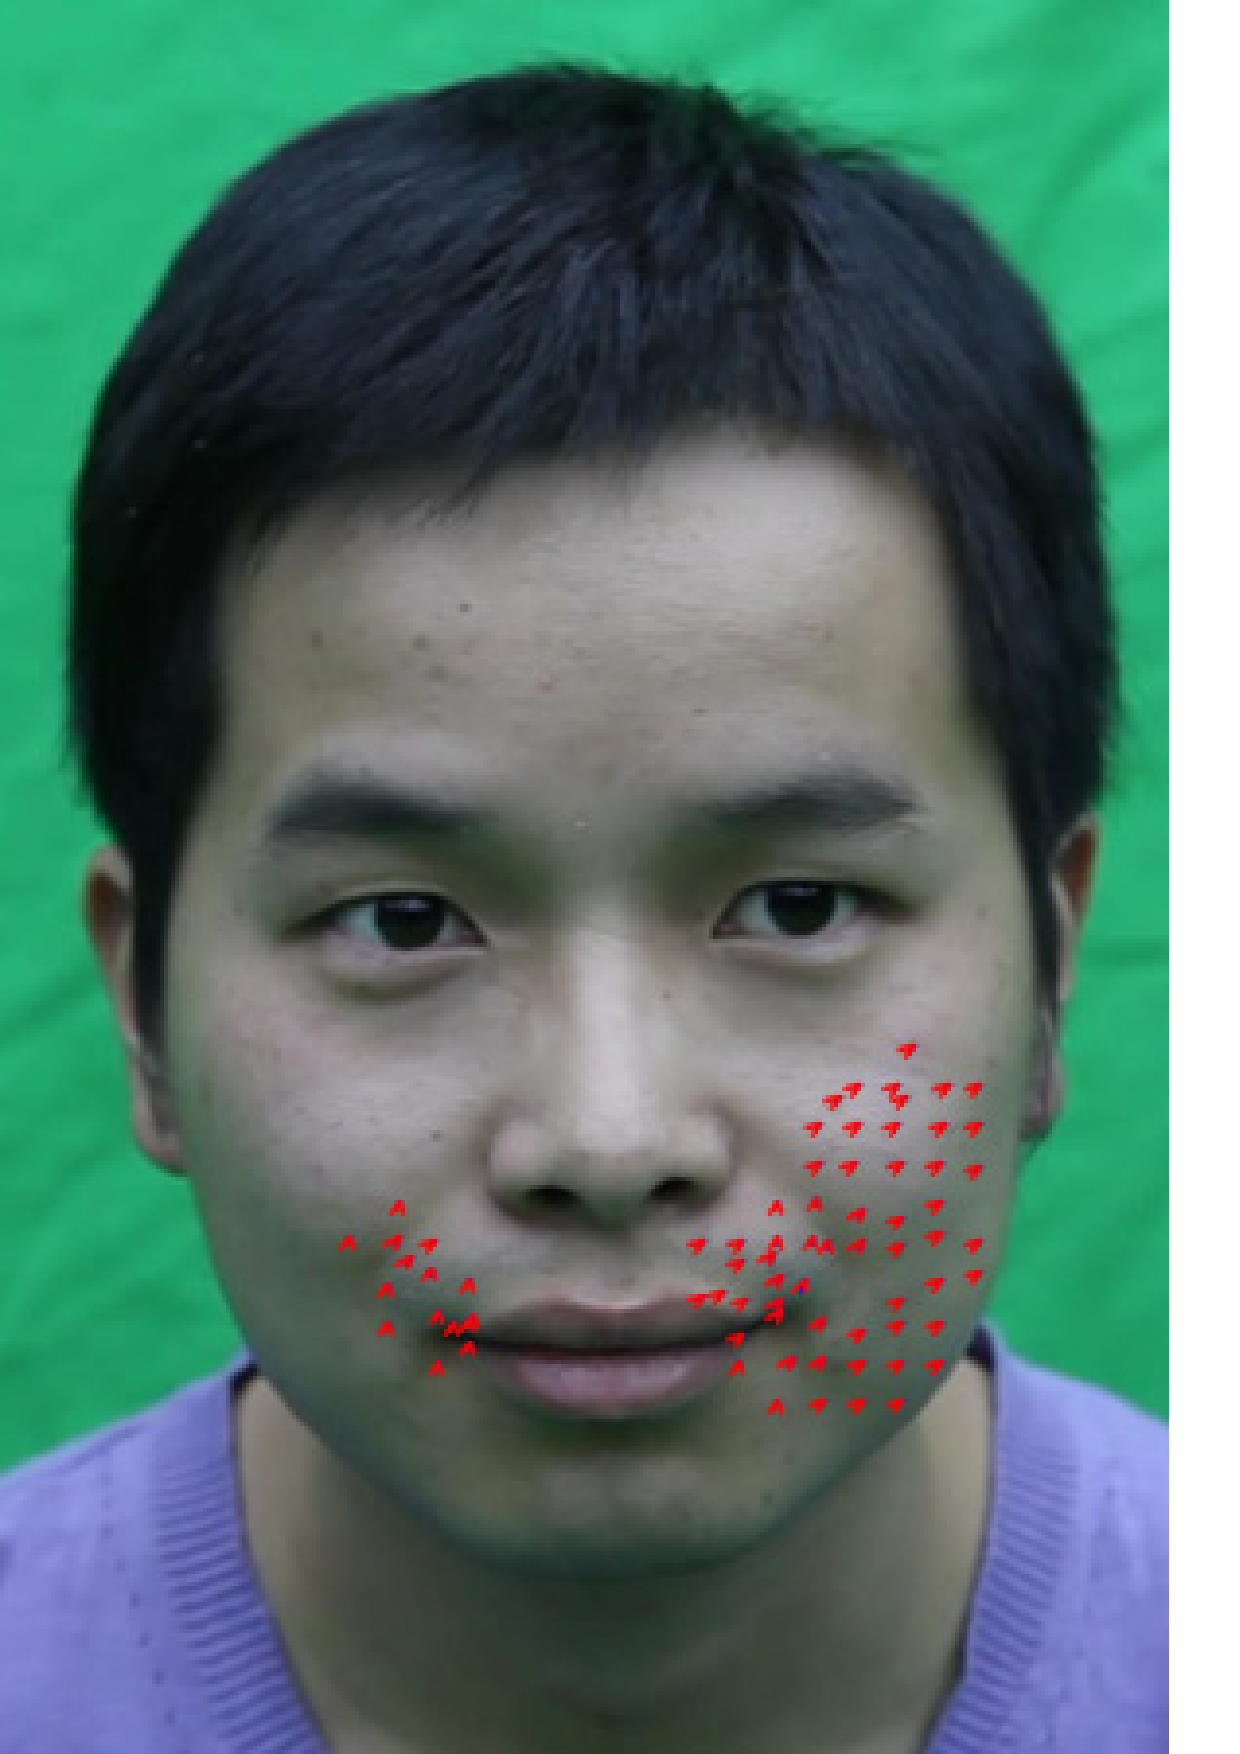
\includegraphics[width=0.205\textwidth]{data/img/velocity_likai_0380_00199_flow.pdf}}
    \subcaptionbox{}{
    \label{fig:velocity_next}
    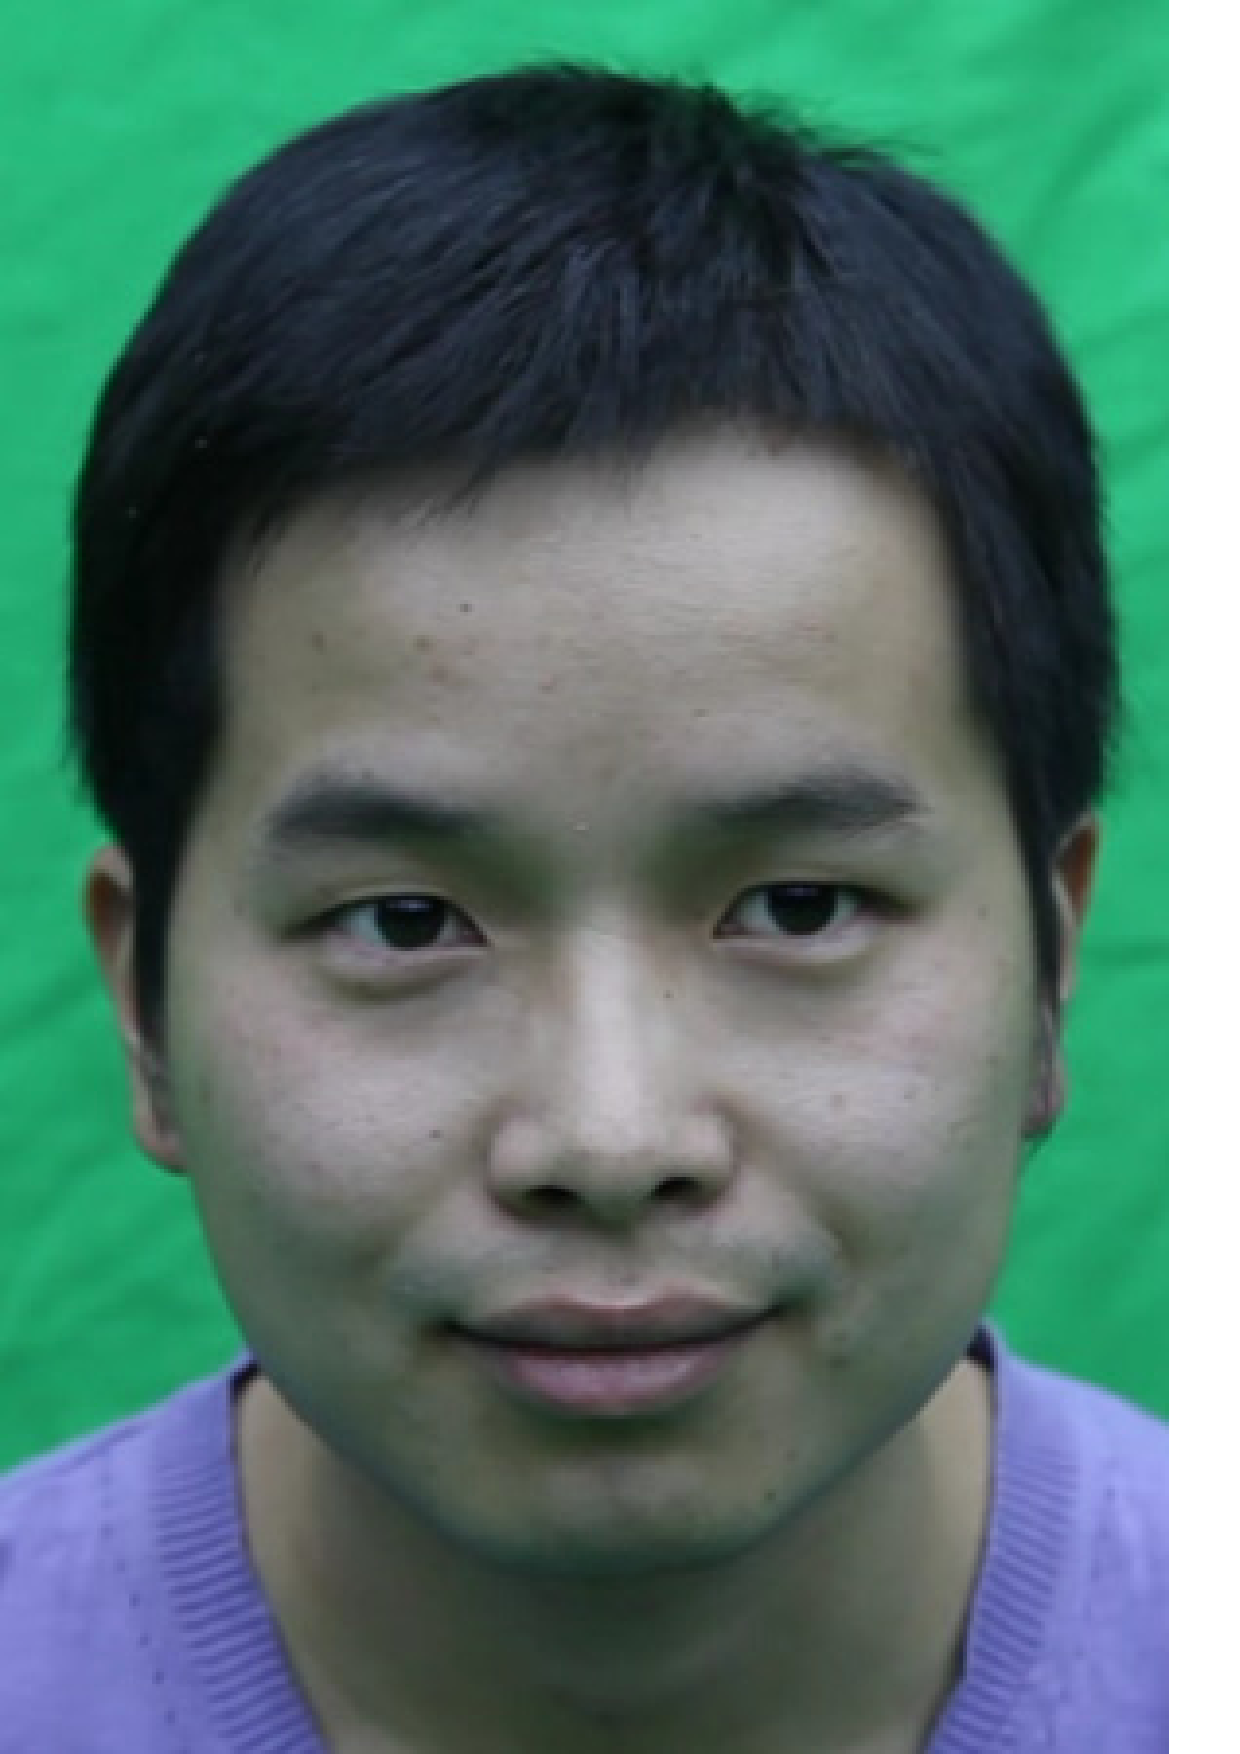
\includegraphics[width=0.205\textwidth]{data/img/velocity_likai_0380_00200.pdf}}
    \subcaptionbox{}{
    \label{fig:velocity_without}
    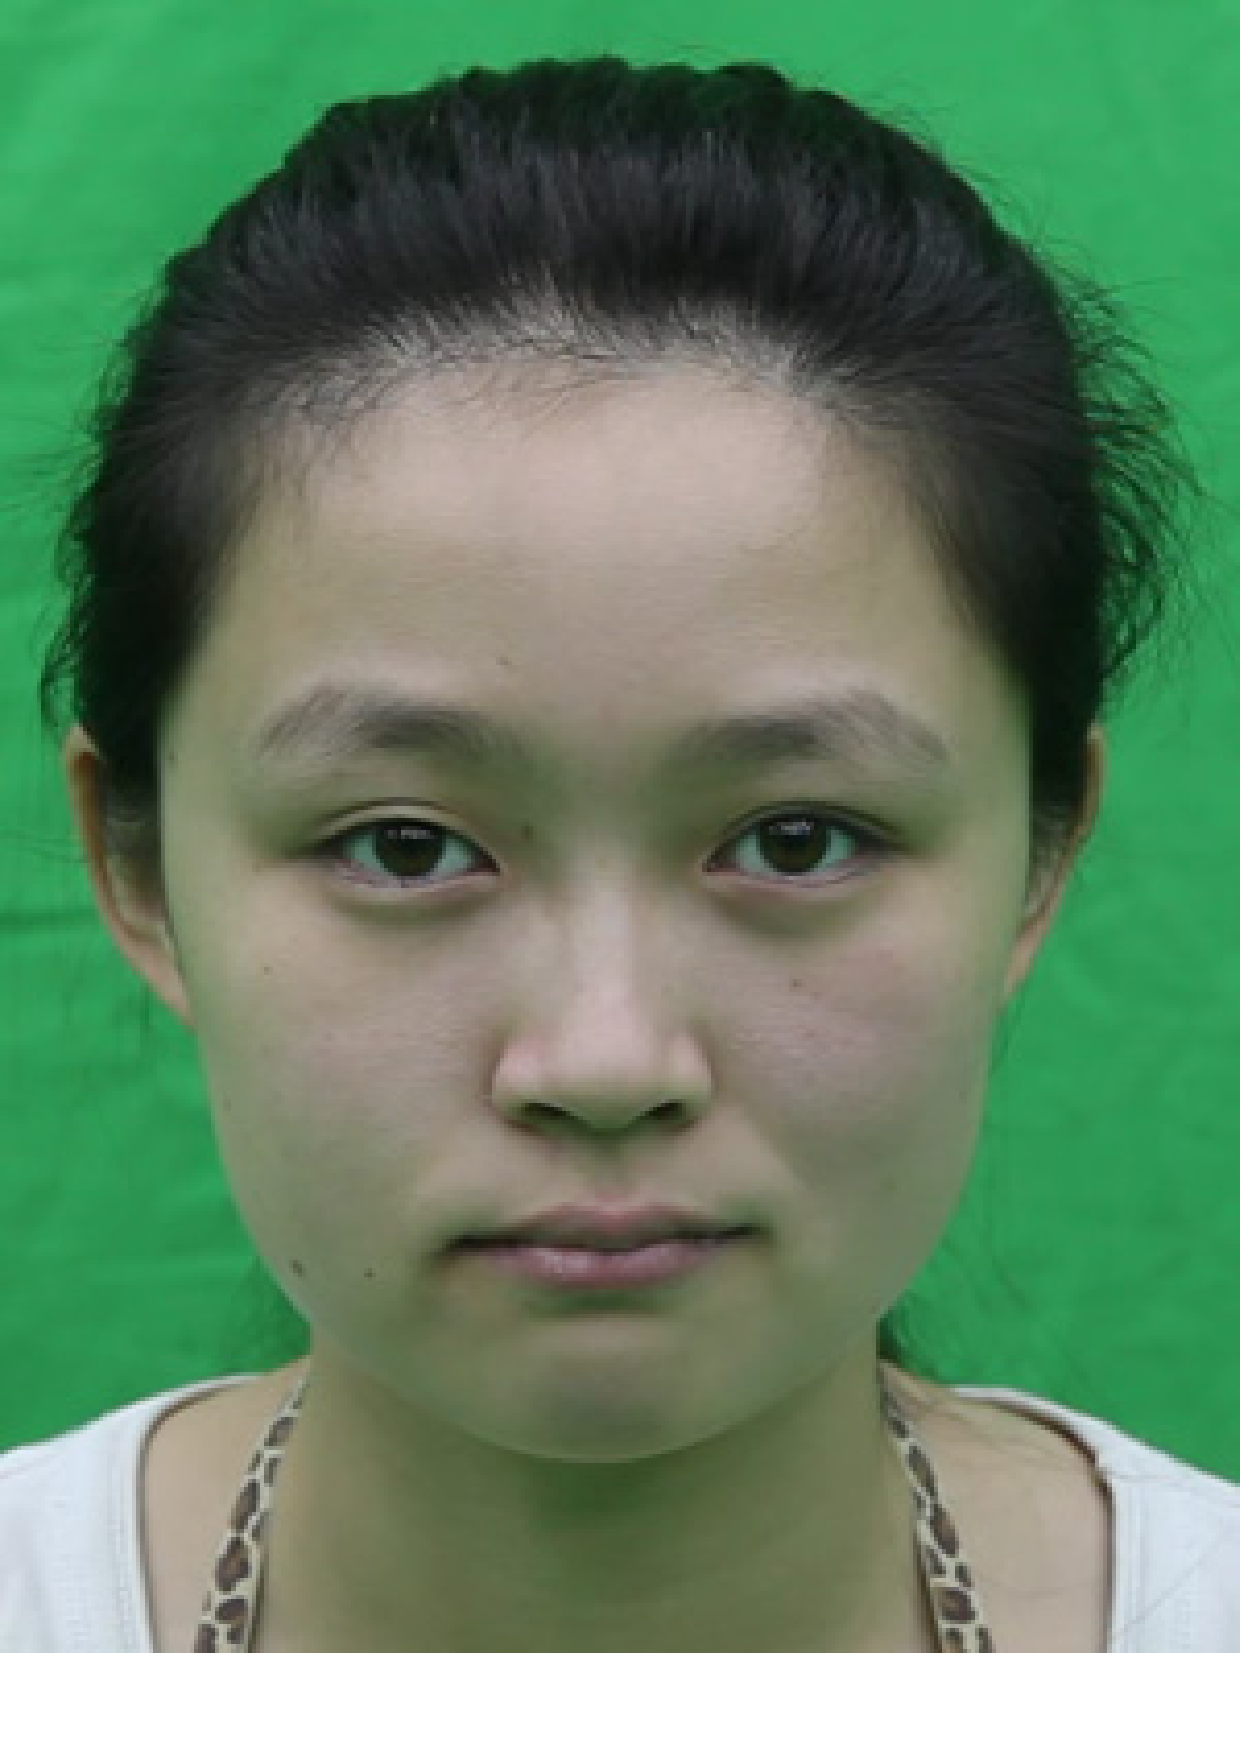
\includegraphics[width=0.23\textwidth]{data/img/velocity_without_00198.pdf}}
    \subcaptionbox{}{
    \label{fig:velocity_with}
    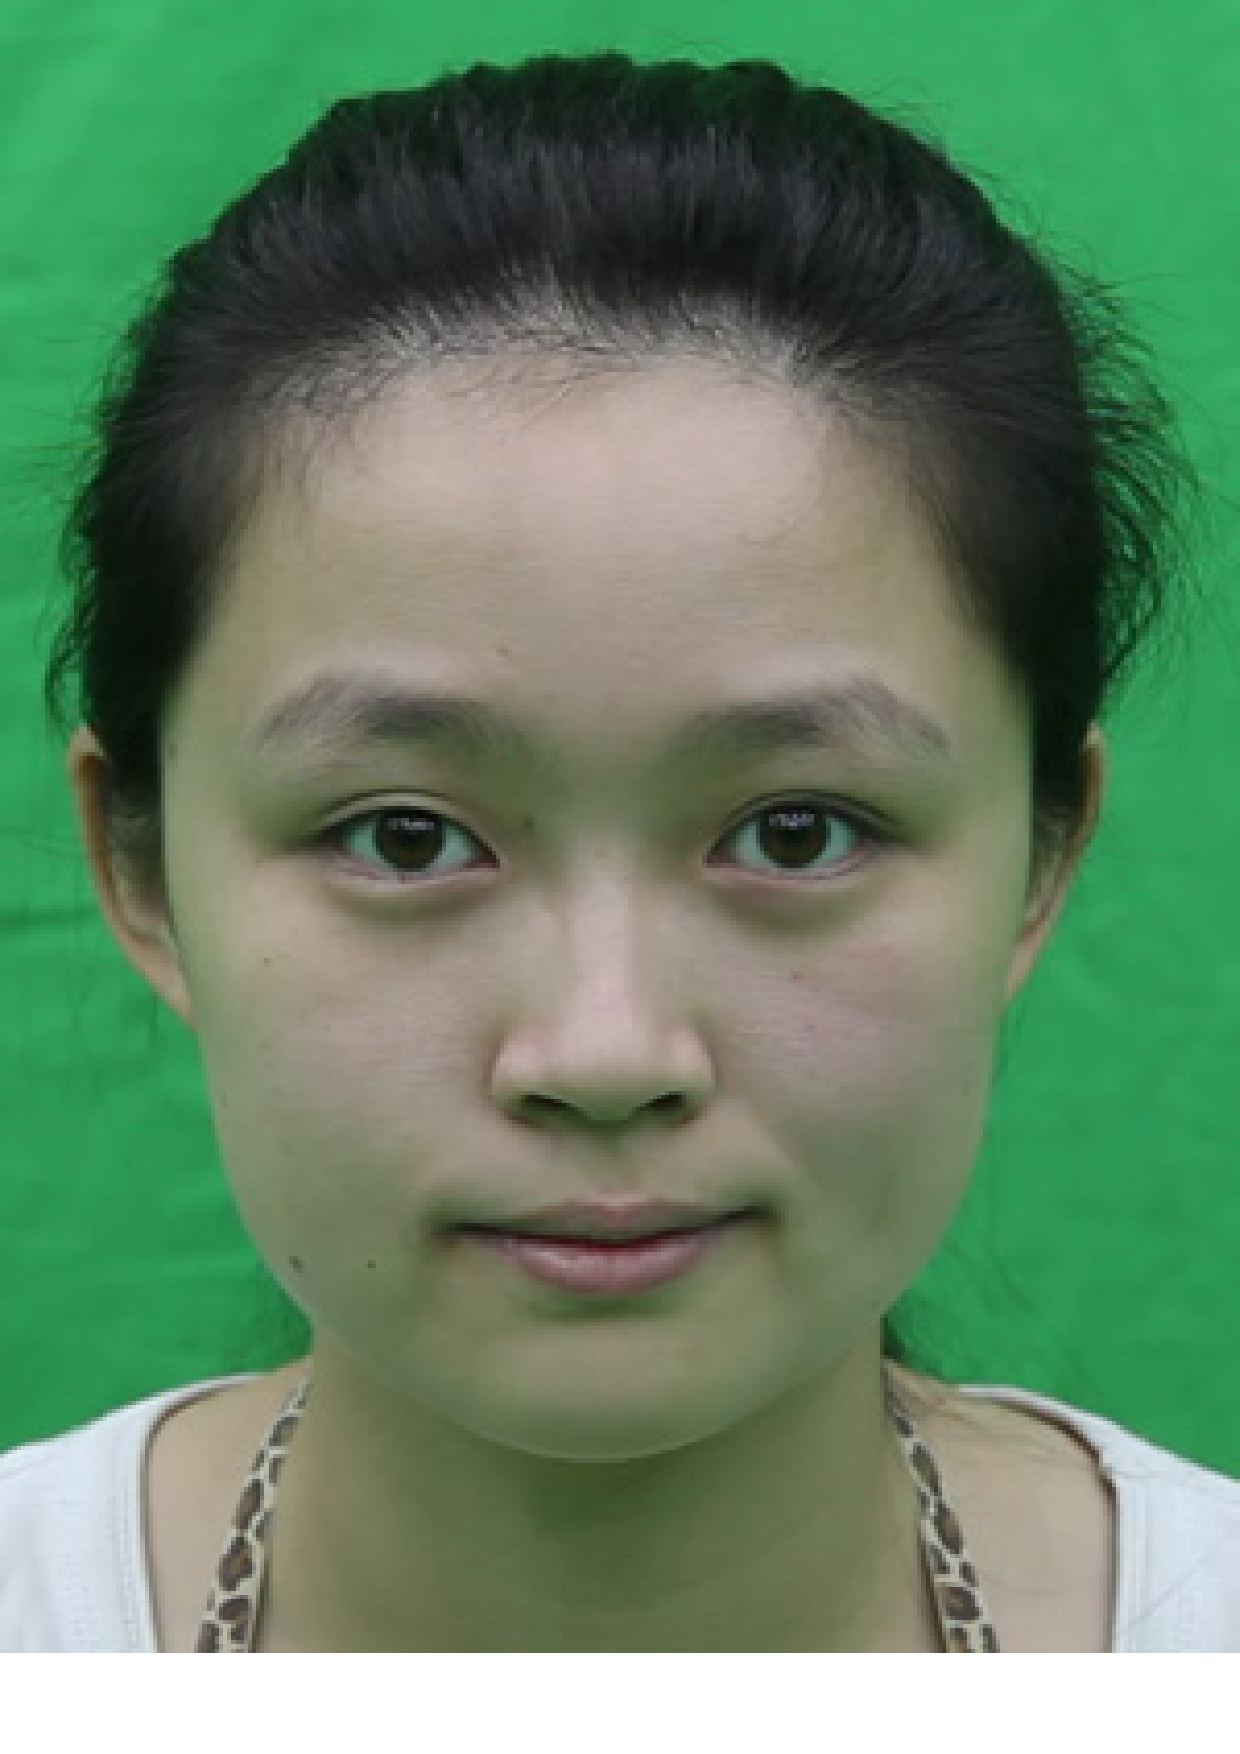
\includegraphics[width=0.23\textwidth]{data/img/velocity_with_00198.pdf}}
    \caption{使用表情速度的重要性阐述。(a) 红色表示带表情速度的当前查询帧。(b) 微笑的下一查询帧。(c) 由公式~\ref{eq:dist_comb}选择的最相似帧,有细淡淡的忧伤。(d)由公式~\ref{eq:dist_all}选择的最相似帧,有正确的微笑。}
    \label{fig:velocity}
\end{figure}

\subsubsection{基于优化的检索}
改进的表情相似度度量不能独立完整地解决时间一致性的问题。因此我们的系统使用就与优化的检索方法进一步提升合成序列的时间一致性。

对于每个查询帧,我们首先使用公式~\ref{eq:dist_all}定义的完整的距离度量从数据库不是抽取一个,而是$k$近邻,我们称之为候选帧。在每帧的时间戳放置一列$k$个候选帧,我们建立如图~\ref{fig:dijkstra}所示的有向无环图。有向边只连接邻近候选帧。记$V_i^{(q)}$ 为时刻$q$ 的第$i$候选帧。我们定义有向弧$r=(V_i^{(q)}, V_j^{(q+1)})$的长度为:
\begin{eqnarray}\label{eq:length}
\mathcal{L}(r)&=&\mathcal{D}(V_i^{(q)},Q_e^{(q)})+
        \mathcal{D}(V_j^{(q+1)},Q_e^{(q+1)})\nonumber\\
        &&+\lambda \exp ( - {{(\mathcal{T}(V_j^{(q + 1)} ) - \mathcal{T}(V_i^{(q)} ) - \mu )^2 }}/{{\sigma ^2 }}),
\end{eqnarray}

这里$\mathcal{T}(\cdot)$是输入帧的时间戳。通过最小化相邻帧的时间差,公式~\ref{eq:length} 的最后一项鼓励数据库中的连续帧选为匹配帧,以保证时间一致性。时间尺度变量$\mu$ 用于补偿查询和数据库序列之间的运动速度差。当查询帧和数据库序列运动速度大致相同,$\mu$设为1,当查询帧运动速度比数据库序列快则设为一个大数,否则相反。$\sigma$是带宽,$\lambda$是时间项的权重。

在公式~\ref{eq:length}中的时间项是L2范数,允许晓得时间变化,但对大的变化有严惩。由于小的变化被允许,它也允许某些时间尺度的变化。这在我们的查询序列1中被证明,如图~\ref{fig:result12}所示,它包含缓慢嘴巴张开的表情和快速撅嘴的表情。我们的系统对这二者都处理很好。此外,$\mu$也能在视频的不同时间根据查询运动的速度自动调整。

\begin{figure}[htbp]
\centering
    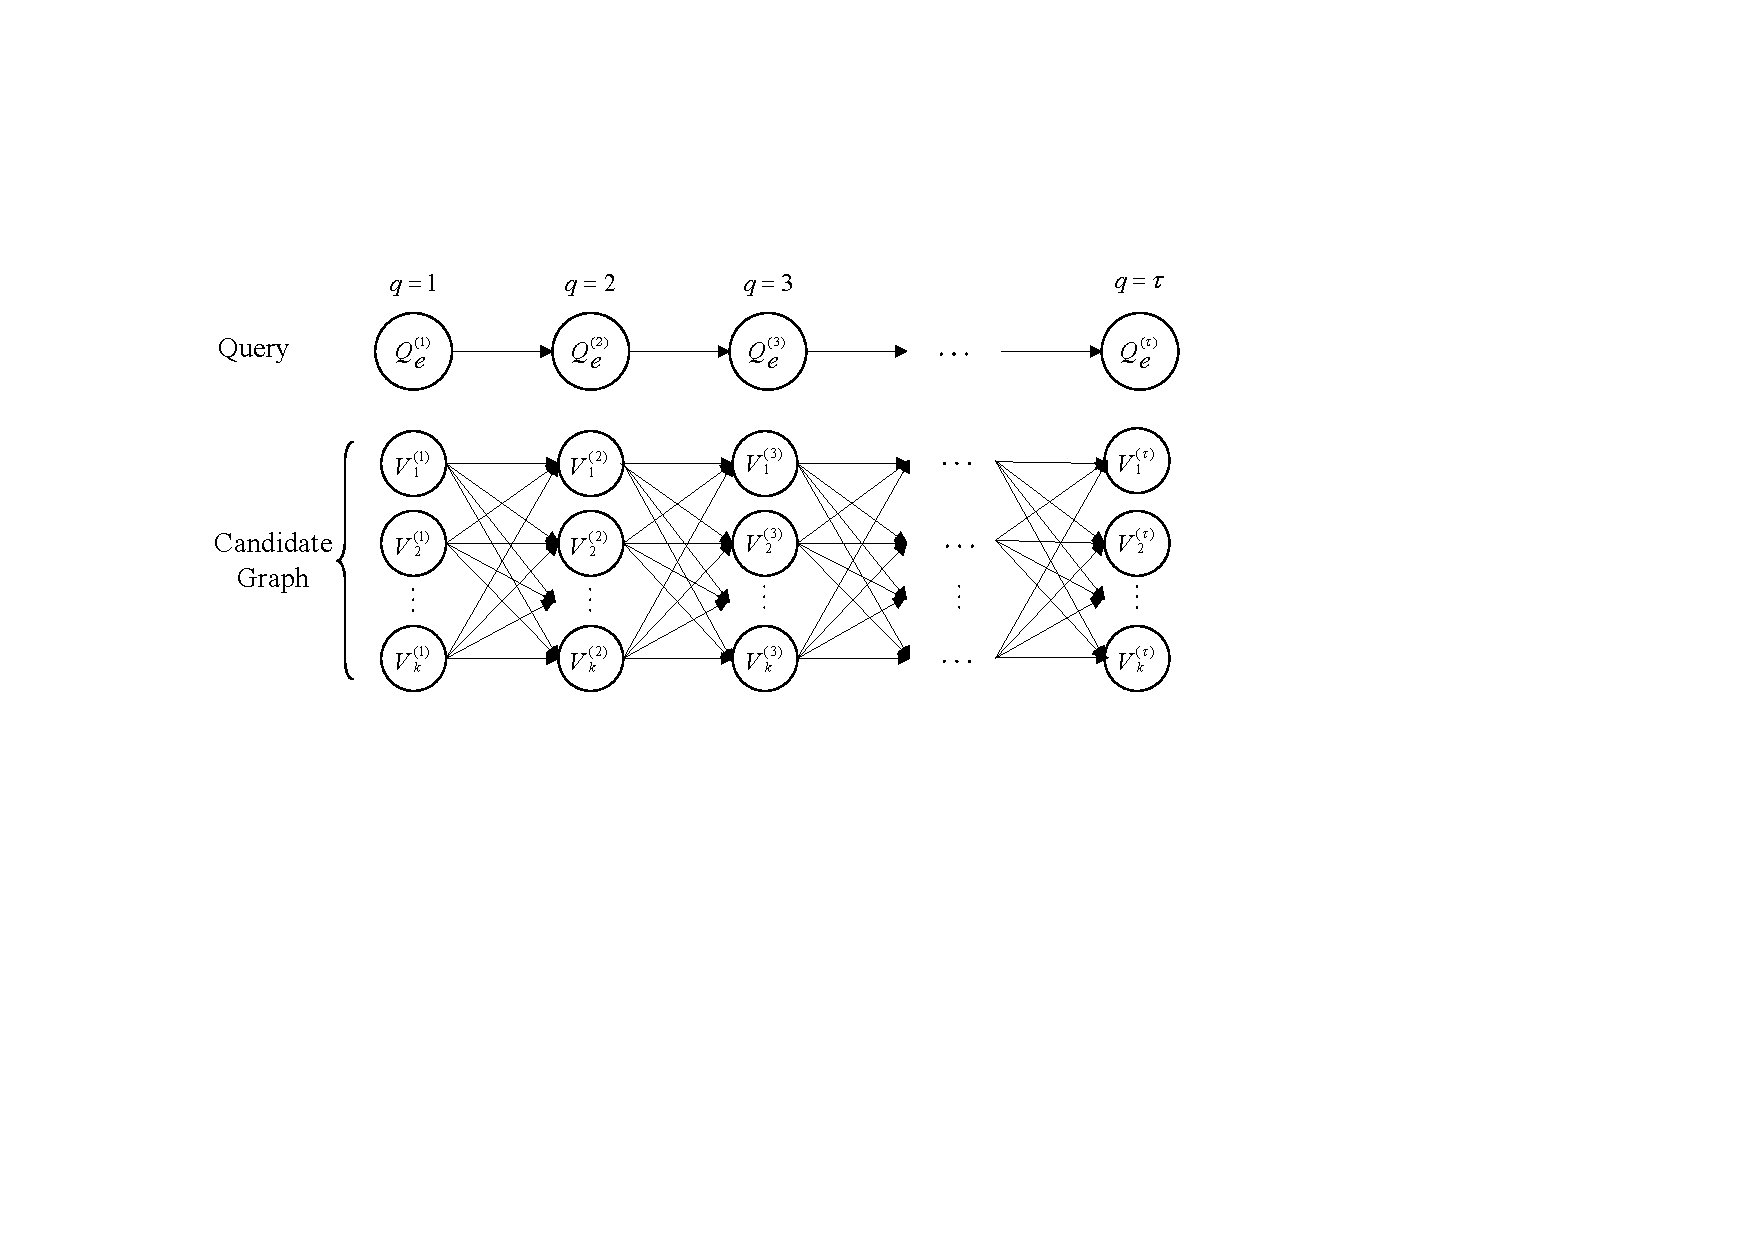
\includegraphics[width=0.90\textwidth]{data/img/dijkstra.pdf}
    \caption{用于检索的有向图}
    \label{fig:dijkstra}
\end{figure}

令$\mathcal{P}_{V_i^{(1)}\to V_j^{(\tau)}}$为连接起始节点$V_i^{(1)}$和终止节点$V_j^{(\tau)}$的路径,这里$i,j\in\{1,2,\ldots,k\}$。
在所有从第一到最后帧的可能路径中,我们找到最短路。优化目标被正式定义如下:
\begin{eqnarray}\label{eq:dijkstra}
\mathcal{P}_{opt}=\mathop{\arg\min}_{i, j} \mathop{\arg\min}_{\mathcal{P}_{V_i^{(1)}\to V_j^{(\tau)}}}
        \sum_{r\in \mathcal{P}_{V_i^{(1)}\to V_j^{(\tau)}}}\mathcal{L}(r).
\end{eqnarray}

该问题用Fibonacci堆~\cite{algorithm}的Dijkstra算法很好解决。连接最优路径$\mathcal{P}_{opt}$的所有帧构成检索序列。

我们的基于优化的方法借鉴了以往用于生成时间一致动画的工作~\cite{Kovar_Gleicher,spacetime,photobios}。我们的方法结合了时间一致性和语义对应。

\subsection{表情精炼}\label{sec:emi}
前面的检索结果有两个缺点。首先,由于我们的数据库的大小是有限的,检索的帧可能不包含和输入序列完全相同的表情。其次,数据库中的帧没完全对齐,所以检索序列包含了一些少量的时间抖动。要删除这些错误,我们的系统采用了额外的表情细化组成部分。

表情精炼的主要思路是给定$Q_n$ 和$Q_e$,中性帧和人偶师的表情帧,还有$T_n$,目标人的中性帧,我们可以直接从两个源图片中提取表情,并映射到$T_n$来合成新的面部$T_{Q_e}$。该合成的脸部,我们称之为expression mapping image(EMI),有所需的表情,但是也许没有逼真的纹理,尤其当$Q_n$ 和 $Q_e$表情差异很大的时候。另一方面,检索帧有真实的外表,但表情和$Q_e$并不完美匹配。结合EMI和检索帧,我们可以生成最终图片,有逼真的外表和精确匹配的表情。

具体说,我们首先通过把$Q_n$ 和$Q_e$的光流转移到目标帧来扭曲$T_n$。给定点$\vec{a}\in Q_n$,$\vec{a}'\in Q_e$和$\vec{b}\in T_n$ ($\vec{b}=g(\vec{a})$ 如公式~\ref{eq:map2}),我们计算点$\vec{b}'\in T_{Q_e}$ 的颜色如下:
\begin{equation}\label{eq:ratio}
c_{\vec{b}'}=c_{\vec{b}}\frac{c_{\vec{a}'}}{c_{\vec{a}}},
\end{equation}

这里$c_{\{\vec{a},\vec{a}',\vec{b},\vec{b}'\}}$分别是点$\vec{a}$, $\vec{a}'$, $\vec{b}$ and $\vec{b}'$的颜色值(我们系统中使用YCrCb颜色空间)。这里我们用比值${c_{\vec{a}'}}/{c_{\vec{a}}}$来表示颜色$c_{\vec{b}}$如ERI方法~\cite{eri}所做。在实际实施中,为了避免$\vec{b}'$有非整数坐标,我们用反向计算表情映射我们从一个整数像素$\vec{b}'\in T_{Q_e}$开始,根据$\vec{a}'=g^{-1}(b')$找到它的对应点$\vec{a}'\in Q_e$ 。通过计算\mbox{\boldmath $F$}$_{Q_e \to Q_n}$获得的光流$\Delta \vec{a}'$ 给出点$\vec{a}$的坐标。通过注册函数,我们获得点$\vec{b}=g(\vec{a})\in Q_n$的位置。然后点$\vec{b}'$ 的颜色可以依据公式\ref{eq:ratio} 计算。

\begin{figure}[htbp]
\centering
    \subcaptionbox{}{
    \label{fig:refine_driven}
    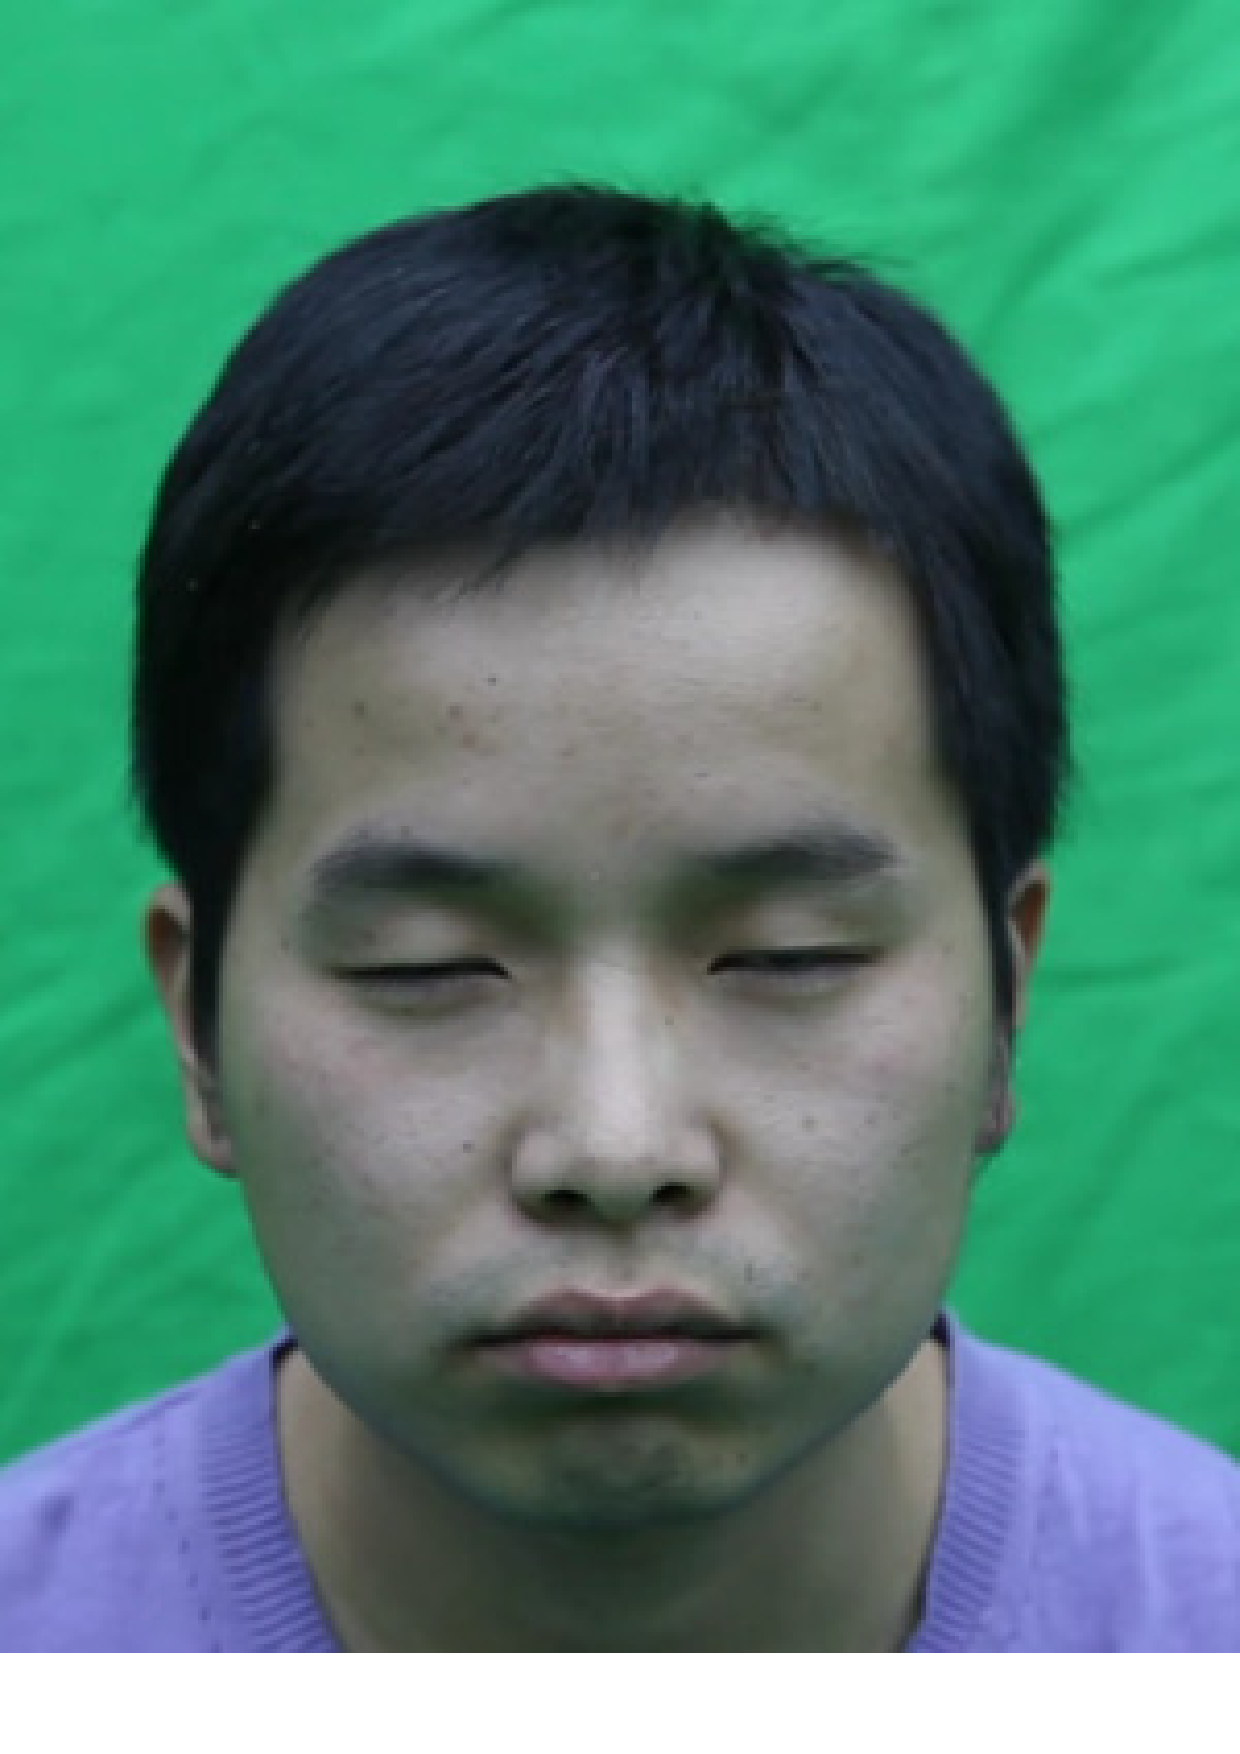
\includegraphics[width=0.23\textwidth]{data/img/refine_likai_0380_00151.pdf}}
    \subcaptionbox{}{
    \label{fig:refine_retrieval}
    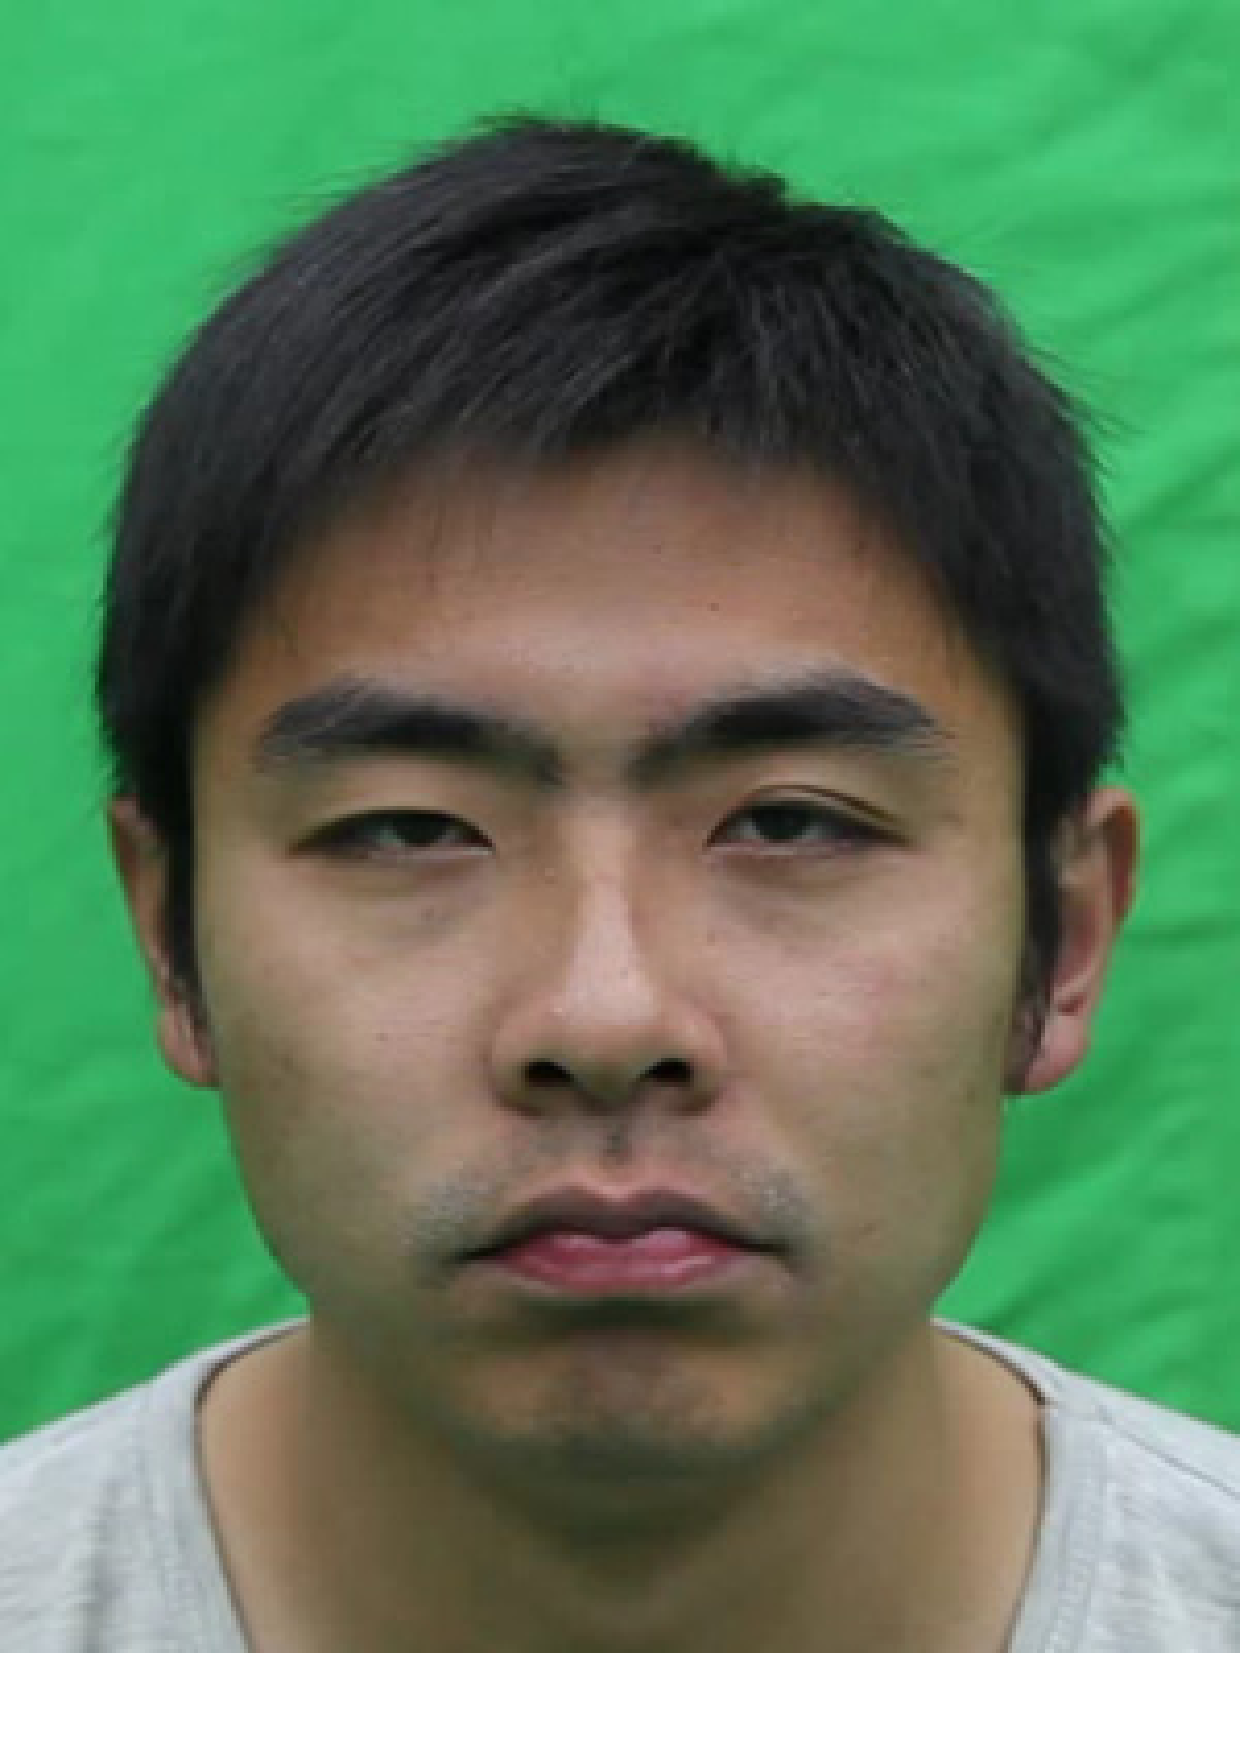
\includegraphics[width=0.23\textwidth]{data/img/refine_retrieval_00150.pdf}}
    \subcaptionbox{}{
    \label{fig:refine_emi}
    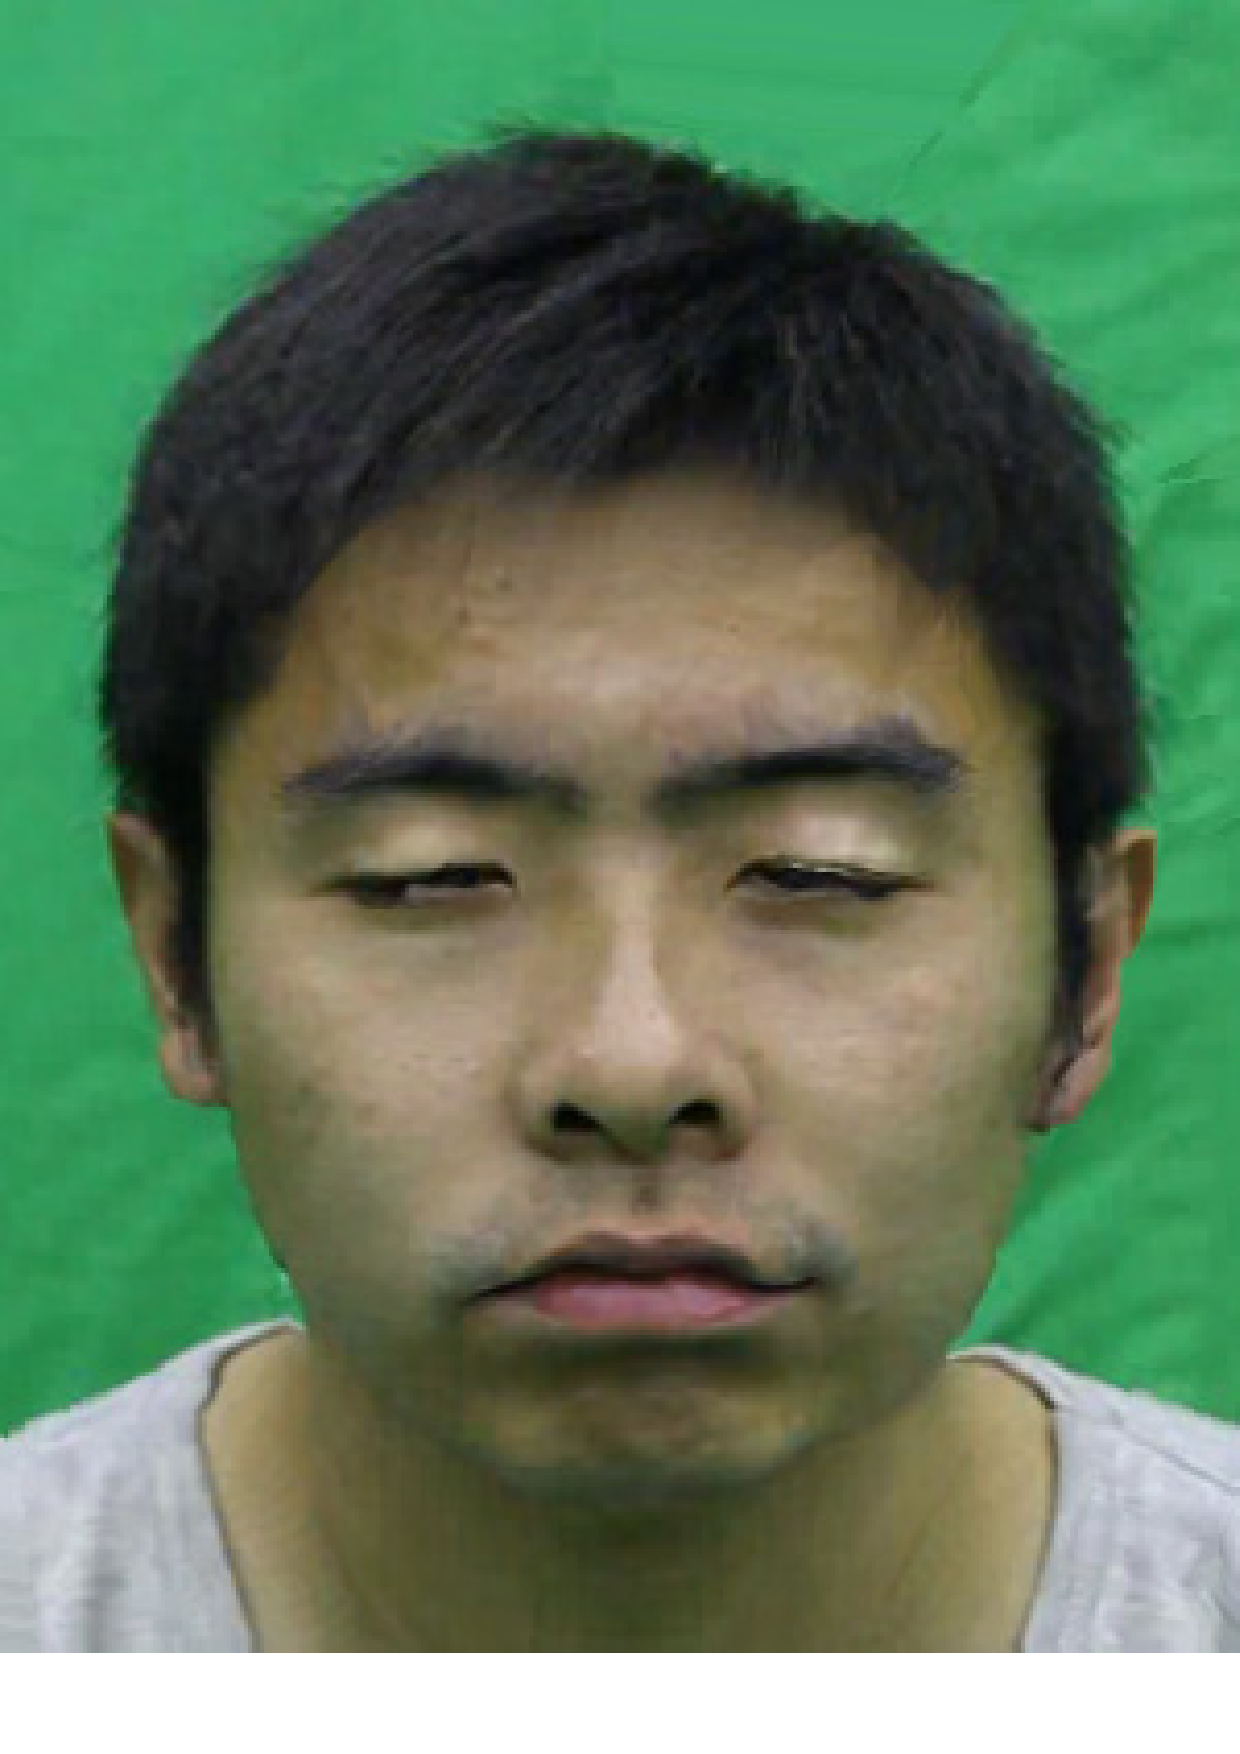
\includegraphics[width=0.23\textwidth]{data/img/refine_EMI_00151.pdf}}
    \subcaptionbox{}{
    \label{fig:refine_final}
    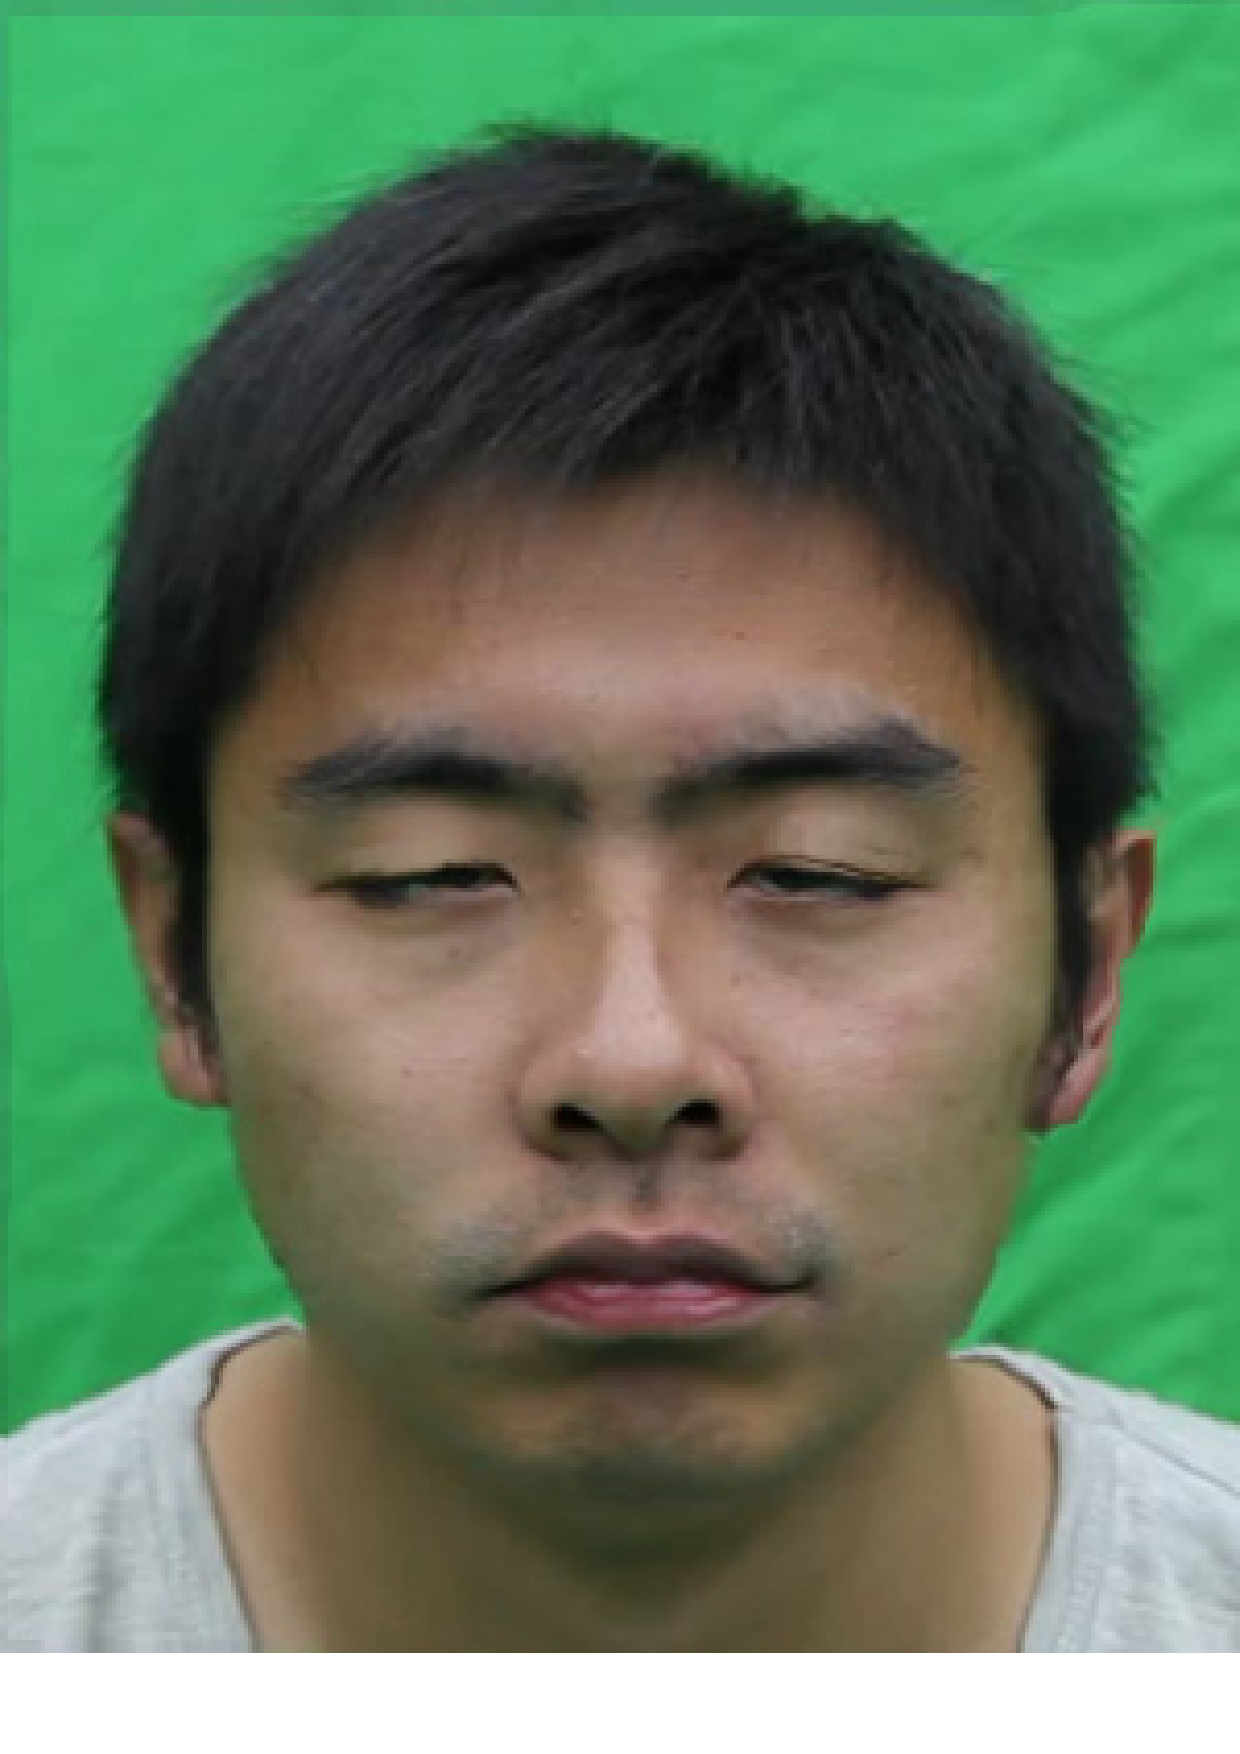
\includegraphics[width=0.23\textwidth]{data/img/refine_combine_00150.pdf}}
    \caption{表情精炼。 (a) 查询帧。 (b) 检索帧。 (c) 表情映射图片。 (d) 最终结果。}
    \label{fig:refine}
\end{figure}

最终,我们计算每一帧时的EMI和检索结果的光流,并利用光流扭曲检索图像至EMI。如图~\ref{fig:refine}所示,最终合成结果不只有从检索帧继承来的真实的外表,还有由EMI图像继承来的和查询帧匹配的正确表情。
\section{结论和讨论}
\begin{figure}[htbp]
\centering
    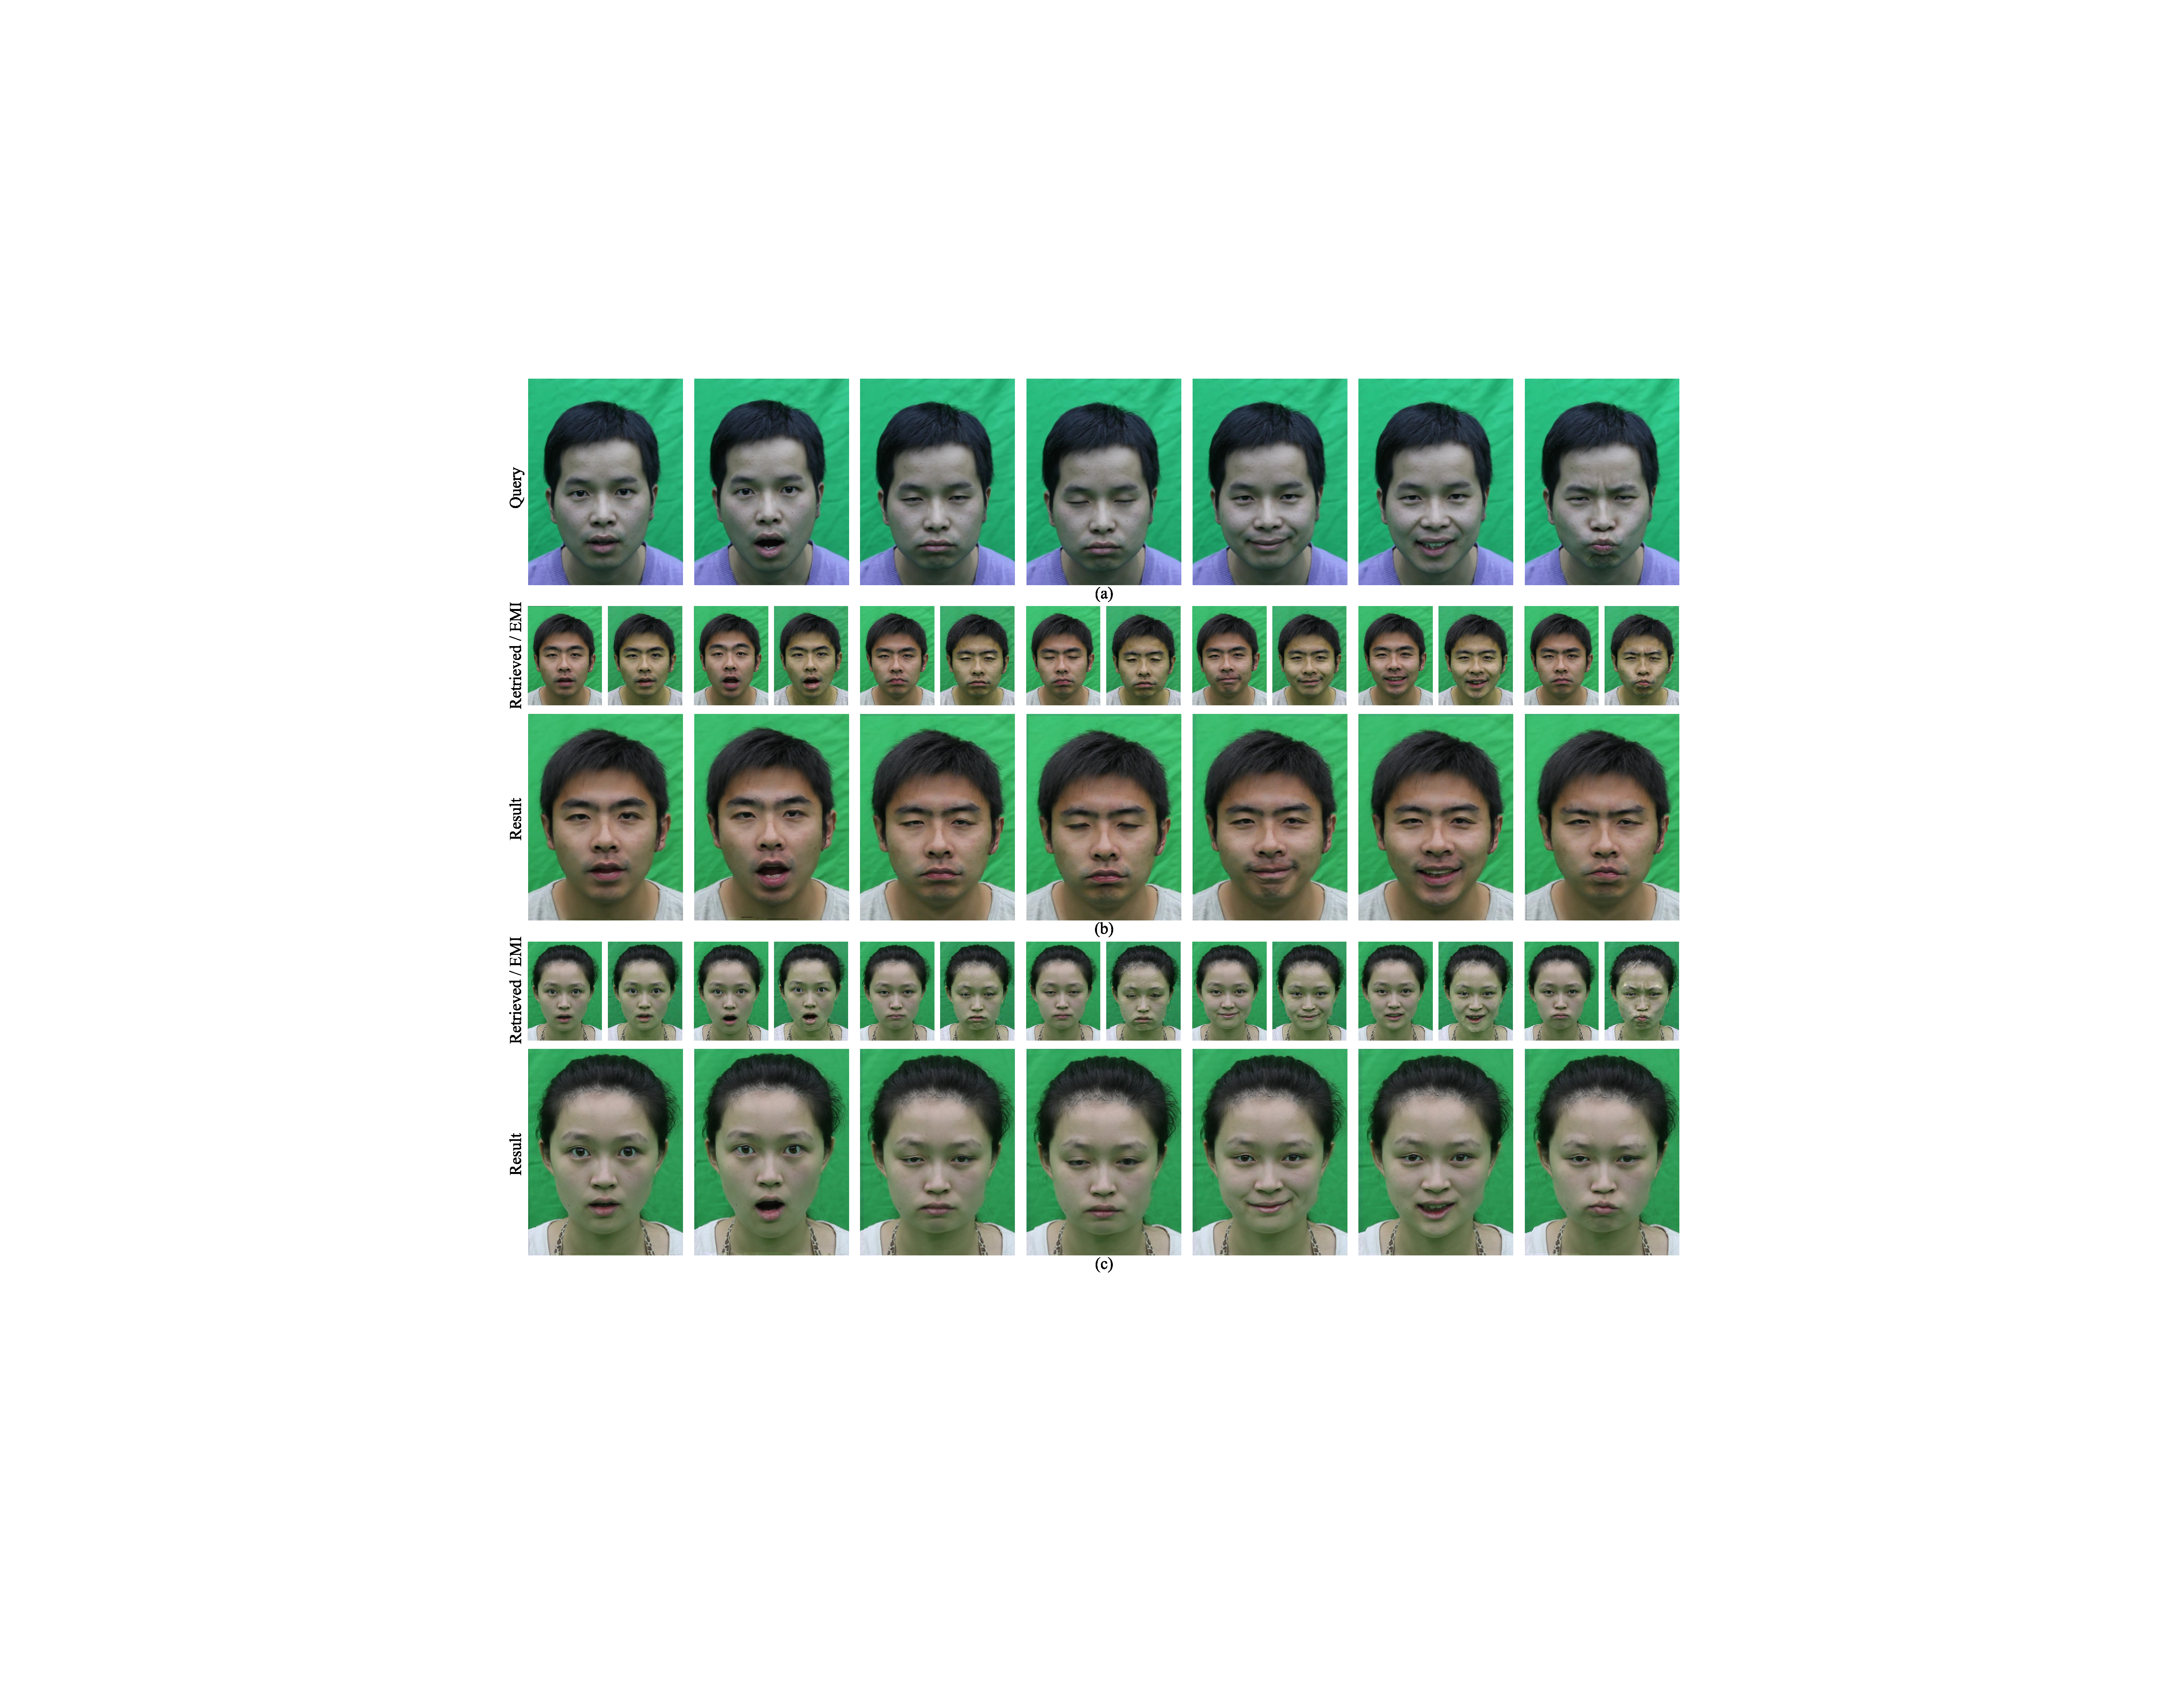
\includegraphics[width=0.9\textwidth]{data/img/likai2xf_jyy.pdf}
    \caption{在目标 $T1$ 和 $T2$ 上运行的查询序列的结果。 (a) 普通查询帧
    (b) (第一行)检索和EMI帧(分别是左和右);(第二行)目标 $T1$ 的最终合成帧。 (c) 目标 $T2$ 的检索、EMI帧和Retrieved最终合成帧。}
    \label{fig:result12}
\end{figure}

\subsection{实验}
我们评估了三个数据库系统。其中两个是我们采集的,这两个主题一个是男性,一个女性,他们被要求表现6个基本表情:愤怒,厌恶,惊讶,恐惧,快乐和悲伤。每个数据库都是25fps拍摄,包含约1500帧。第三个数据库是从Extended Cohn-Kanade Dataset (CK+) \cite{CK+}得到的 S130 。 S130 中的11个短序列(共220帧)构成了该表情数据库。在所有试验中,我们算法的参数固定如下:$\alpha_e=\frac{0.6}{n_{e}}$, $\alpha_m=\frac{0.4}{n_m}$, $\beta_m=0.9$, $\beta_o=0.1$,
$\gamma_e=0.9$, $\gamma_v=0.1$, $k=20$, $\lambda=0.1$, $\mu=1$, $\sigma=2$,其中 $n_e$ 和 $n_m$ 分别是目标中性面眼镜和嘴巴区域的像素数量。

\subsection{结果和评估}
图~\ref{fig:result12}显示了目标 $T1$(男性)和 $T2$ (女性)由输入序列驱动的合成结果。注意我们的系统不仅在诸如笑脸和惊奇等表情在数据库中时可以合成逼真的表情,而且在诸如撅嘴且双眼紧闭的表情在数据库中没有的时候也能合成新表情。同时,最终合成的视频也是时间相干的。图~\ref{fig:result3}展示了由另一序列驱动,从来自 CK+ 数据库的S130 中合成的结果。结果表明即使只是一个小数据库我们的系统仍然效果很好。可以在补充材料中找到包括额外的快速说话重定位结果的完整的视频序列。
为了评价我们的合成结果,我们进行了包含 $34$ 个参与者的用户研究。每位参与者都被展示了四个视频,分别由 LBP 特征查询方法~\cite{eccv10},在第~\ref{sec:emi}章介绍的 EMI 方法,我们的检索策略和我们的整套算法一帧一帧查询获得。每个视频并排展示了查询和结果。在实验中,参与者被要求根据表情的真实性和一致性评价在每个结果中表情的好坏,分数从 5(非常好)到 0(一点也不好)。表~\ref{tab:userstudy} 显示了3个目标的平均分。参与者发现我们的最终结果是最好的且我们的检索策略优于在~\cite{eccv10}提出的方法。
\renewcommand{\tablename}{表}
\begin{table}[htp]
\centering
    \begin{tabular}{|l|p{1cm}|p{1cm}|p{1cm}|}
    \hline
    & $T1$ & $T2$ & S130\\
    \hline\hline
    基于 LBP 的检索 \cite{eccv10} & 1.20 & $1.50$ & $1.38$\\
    我们的检索 & $2.49$ & $3.00$ & $2.56$\\
    EMI & $2.89$ & $1.91$ & $3.35$\\
    我们的整套系统 & $\mathbf{4.02}$ & $\mathbf{4.56}$ & $\mathbf{4.08}$\\
    \hline\hline
    $p$ 值 & $0.002$ & $0.005$ & $0.0001$ \\
    \hline
    \end{tabular}
    \caption{用户研究结果。该结果在统计上是有意义的,使用了单变量方差分析,$p$-value $<0.01$。}
    \label{tab:userstudy}
\end{table}

\subsection{局限性}
我们目前的系统只针对正面脸部表情合成设计。可能会扩展系统在大旋转角下运行,通过稀疏相机阵列采集数据。如此我们需要估计表情和输入帧的3D脸部。此外,需要视图变形技术~\cite{ViewMorphing}来在不同视角查看脸部,以在所需姿态生成面部表情。

另一个限制是,当表情很极端,传统的光溜方法无法精确捕捉表情差异。除了调查更好的脸部光流技术,另一个解决方案是为每个特征使用多个预先对其的脸部图像而不只是在我们现有系统中使用单一中性面。

\begin{figure*}[htbp]
\centering
    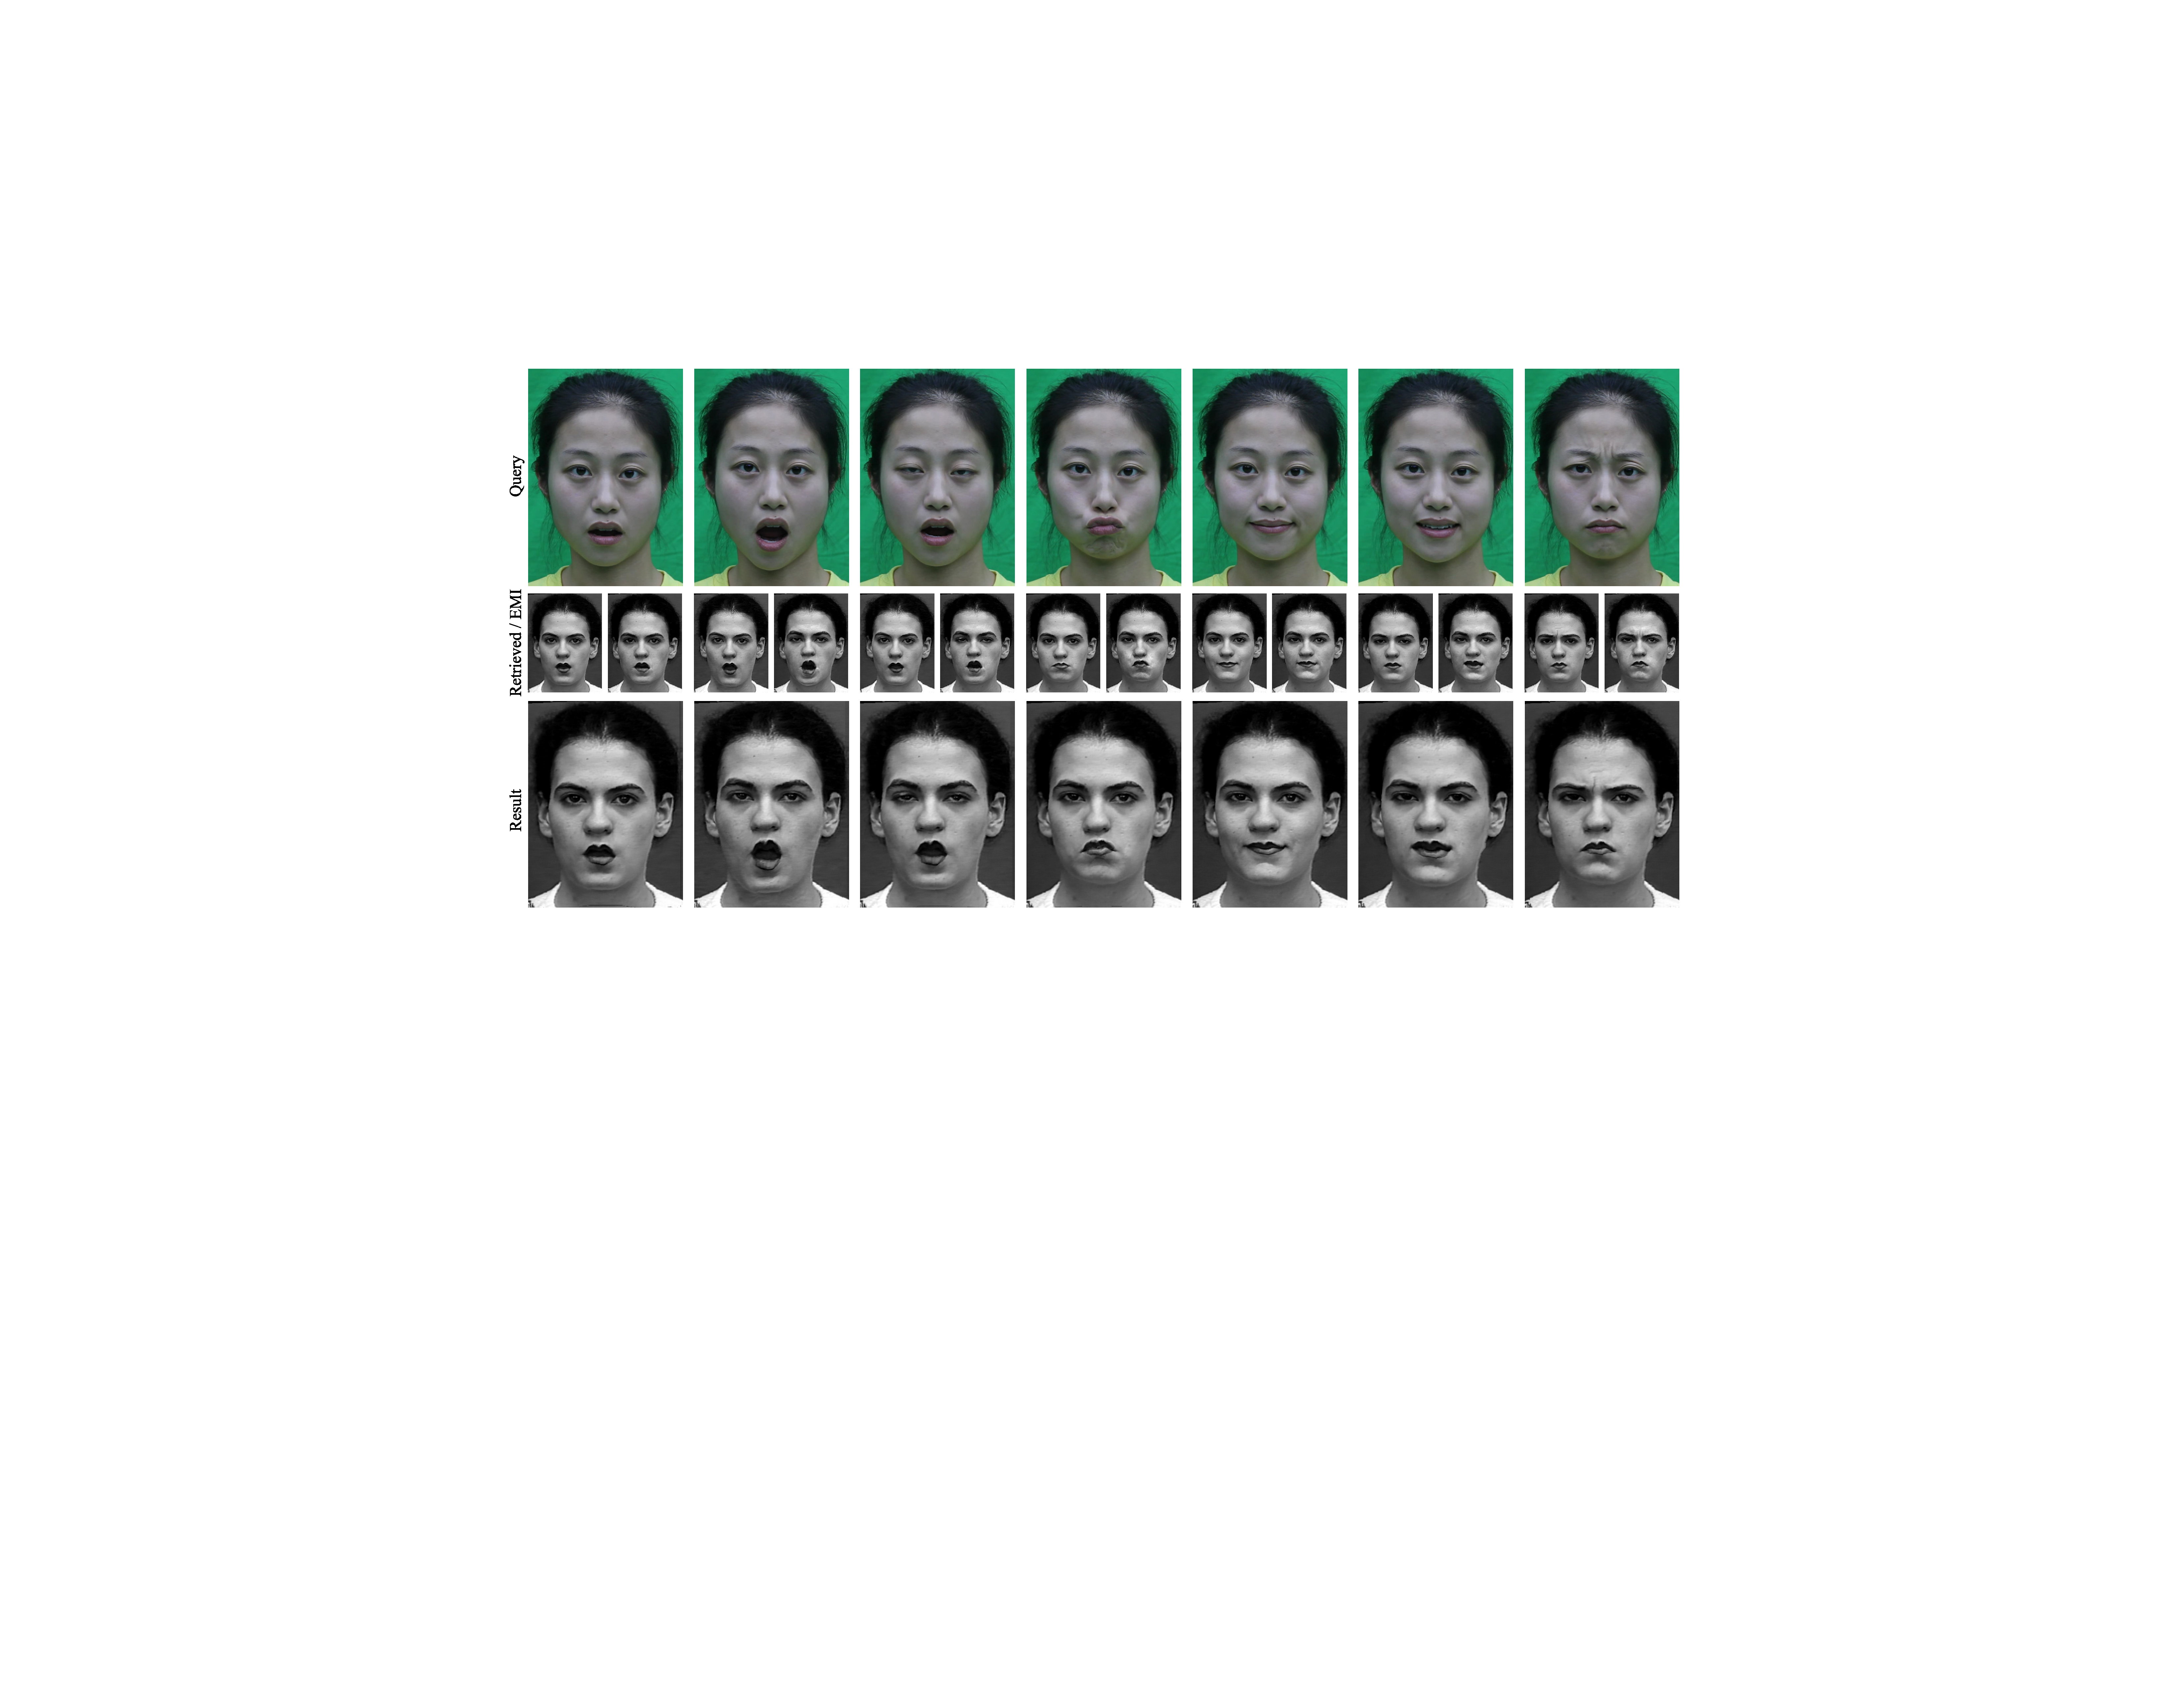
\includegraphics[width=0.90\textwidth]{data/img/liwen2S130.pdf}
    \caption{在来自CK+的S130中由查询序列2获得的结果。 (顶部)查询帧。(中部)检索帧和EMI 帧(分别是左和右)。(底部)最终合成帧。}
    \label{fig:result3}
\end{figure*}

\section{结论}

我们提出了一种数据驱动的方法来用一个人的面部表情视频对目标人脸合成真实的面部动画。我们的系统采用了新颖的时空表情距离度量,可以准确地测量视频中不同的人相似的表情。我们也提出了最短路径优化的检索策略来平衡在最终视频的表情相似性和时间连续性。和那些直接表情映射相比,通过变换检索到的视频帧进一步改善了表情相似性。用户研究结果表明,我们的系统可以产生很高的保真度和时间上一致的面部动画。

\section*{致谢}
作者要感谢和王瑞平,邓岳,索津莉的讨论,评审和领导建设性的意见。这项研究由国家自然科学基金项目支持(第61035002号,第61073072号,第60933006号)。

\setcounter{NAT@ctr}{0}%
\renewcommand{\refname} {参考文献}
{\small
\bibliographystyle{ieee}
\pagestyle{empty}
\bibliography{egbib}
}

% \end{appendix}
%
% % 个人简历
% \begin{resume}

  \resumeitem{个人简历}

  xxxx 年 xx 月 xx 日出生于 xx 省 xx 县。
  
  xxxx 年 9 月考入 xx 大学 xx 系 xx 专业,xxxx 年 7 月本科毕业并获得 xx 学士学位。
  
  xxxx 年 9 月免试进入 xx 大学 xx 系攻读 xx 学位至今。

  \resumeitem{发表的学术论文} % 发表的和录用的合在一起

  \begin{enumerate}[{[}1{]}]
  \item Yang Y, Ren T L, Zhang L T, et al. Miniature microphone with silicon-
    based ferroelectric thin films. Integrated Ferroelectrics, 2003,
    52:229-235. (SCI 收录, 检索号:758FZ.)
  \item 杨轶, 张宁欣, 任天令, 等. 硅基铁电微声学器件中薄膜残余应力的研究. 中国机
    械工程, 2005, 16(14):1289-1291. (EI 收录, 检索号:0534931 2907.)
  \item 杨轶, 张宁欣, 任天令, 等. 集成铁电器件中的关键工艺研究. 仪器仪表学报,
    2003, 24(S4):192-193. (EI 源刊.)
  \item Yang Y, Ren T L, Zhu Y P, et al. PMUTs for handwriting recognition. In
    press. (已被 Integrated Ferroelectrics 录用. SCI 源刊.)
  \item Wu X M, Yang Y, Cai J, et al. Measurements of ferroelectric MEMS
    microphones. Integrated Ferroelectrics, 2005, 69:417-429. (SCI 收录, 检索号
    :896KM.)
  \item 贾泽, 杨轶, 陈兢, 等. 用于压电和电容微麦克风的体硅腐蚀相关研究. 压电与声
    光, 2006, 28(1):117-119. (EI 收录, 检索号:06129773469.)
  \item 伍晓明, 杨轶, 张宁欣, 等. 基于MEMS技术的集成铁电硅微麦克风. 中国集成电路, 
    2003, 53:59-61.
  \end{enumerate}

  \resumeitem{研究成果} % 有就写,没有就删除
  \begin{enumerate}[{[}1{]}]
  \item 任天令, 杨轶, 朱一平, 等. 硅基铁电微声学传感器畴极化区域控制和电极连接的
    方法: 中国, CN1602118A. (中国专利公开号.)
  \item Ren T L, Yang Y, Zhu Y P, et al. Piezoelectric micro acoustic sensor
    based on ferroelectric materials: USA, No.11/215, 102. (美国发明专利申请号.)
  \end{enumerate}
\end{resume}

%
% \end{document}
% \end{example}
%
% \subsection{选项}
% \label{sec:option}
% 本模板提供了一些选项以方便使用:
% \begin{description}
% \item[bachelor]
%   如果写本科论文将此选项打开。
%   \begin{example}
% \documentclass[bachelor]{thuthesis}
%   \end{example}
%
% \item[master]
%   如果写硕士论文将此选项打开。
%   \begin{example}
% \documentclass[master]{thuthesis}
%   \end{example}
%
% \item[doctor]
%   如果写博士论文将此选项打开。
%   \begin{example}
% \documentclass[doctor]{thuthesis}
%   \end{example}
%
% \item[postdoctor]
%   如果写博士博士后出站报告将此选项打开。
%   \begin{example}
% \documentclass[postdoctor]{thuthesis}
%   \end{example}
%
% \item[secret]
%   涉秘论文开关。配合另外两个命令 |\secretlevel| 和 |\secretyear| 分别用来指定保
%   密级别和时间。二者默认分别为\textbf{秘密}和当前年份。可以通过:
%   \cs{secretlevel}|{|绝密|}| 和 \cs{secretyear}|{|10|}| 年独立修改。
%   \begin{example}
% \documentclass[bachelor, secret]{thuthesis}
%   \end{example}
%
% \changes{v3.0}{2007/05/12}{不用专门为本科论文生成\textbf{提交}版本了。}
%
% \item[openany, openright]
%   正规出版物的章节出现在奇数页,也就是右手边的页面,这就是 \texttt{openright},
%   也是 \thuthesis 的默认选项。在这种情况下,如果前一章的最后一页也是奇数,那么
%   模板会自动生成一个纯粹的空白页,很多人不是很习惯这种方式,而且学校的格式似乎
%   更倾向于页面连续,那就是通常所说的 \texttt{openany}。{\fangsong 目前所有论文都是
%      openany。}这两个选项不用专门设置,\thuthesis{} 会根据当前论文类型自动选
%   择。
%
% \item[winfonts,adobefonts,nofonts]
%   这些选项用来指导 ctex 宏包/文档类设置选用的中文字体。
%   winfonts 指定使用中易的六款字体(XeTeX 下为四种)。adobefonts 指定使用 Adobe 的
%   四款免费中文字体,nofonts 不提供可用的中文字体,由用户自行设定。
%
% \item[arial]
%   使用真正的 arial 字体。此选项会装载 arial 字体宏包,如果此宏包不存在,就装
%   载Helvet。arialtoc 和 arialtitle 不受 arial 的影响。因为一般的 \TeX{} 发行都
%   没有 arial 字体,所以默认采用 Helvet,因为二者效果非常相似。如果你执着的要
%   用arial 字体,请参看:\href{http://www.mail-archive.com/ctan-ann@dante.de/msg00627.html}{Arial
%     字体}。
%
% \item[arialtoc]
%  目录项(章目录项除外)中的英文是否用 arial 字体。本选项和下一个 \textsl{arialtitle} 都不用用户
%  操心,模板都自动设置好了。
%
% \item[arialtitle]
%  章节标题中英文是否用 arial 字体(默认打开)。
% \end{description}
%
% \subsection{字体配置}
% \label{sec:font-config}
% 正确配置中文字体是使用模板的第一步。模板调用 ctex 宏包,提供如下字体使用方式:
% \begin{itemize}
%   \item 基于传统 CJK 包,使用 latex、pdflatex 编译;
%   \item 基于 xeCJK 包,使用 xelatex 编译。
% \end{itemize}
%
% 第一种方式的字体配置比较繁琐,建议使用 donated 制作的中文字体包(自
% 包含安装方法),请用户自行下载安装,此处不再赘述。本模板推荐使用第二
% 种方法,只要把所需字体放入系统字体文件夹(也可以指定自定义文件夹)即
% 可。用户可以使用 winfonts,adobefonts,nofonts 选项来选择可用的中文字库,
% 缺省情况下为 winfonts 有效,使用中易字体。注意当使用 xelatex 编译时,
% winfonts 只有中易的四款字体(宋体、黑体、楷书和仿宋)可用,而本科生需要用到幼圆,
% 另外 Linux 系统缺少上述字体,这些用户可以通过指定 nofonts 选项,利用 fontname.def
% 文件配置所需字体。使用中易六种字体的配置如下:
% \begin{example}
% \ProvidesFile{fontname.def}
% \setCJKmainfont[BoldFont={SimHei},ItalicFont={KaiTi}]{SimSun}
% \setCJKsansfont{SimHei}
% \setCJKmonofont{FangSong}
% \setCJKfamilyfont{zhsong}{SimSun}
% \setCJKfamilyfont{zhhei}{SimHei}
% \setCJKfamilyfont{zhkai}{KaiTi}
% \setCJKfamilyfont{zhfs}{FangSong}
% \setCJKfamilyfont{zhli}{LiSu}
% \setCJKfamilyfont{zhyou}{YouYuan}
% \newcommand*{\songti}{\CJKfamily{zhsong}} % 宋体
% \newcommand*{\heiti}{\CJKfamily{zhhei}}   % 黑体
% \newcommand*{\kaishu}{\CJKfamily{zhkai}}  % 楷书
% \newcommand*{\fangsong}{\CJKfamily{zhfs}} % 仿宋
% \newcommand*{\lishu}{\CJKfamily{zhli}}    % 隶书
% \newcommand*{\youyuan}{\CJKfamily{zhyou}} % 幼圆
% \end{example}
%
% 对 Windows XP 来说如下,KaiTi 需要替换为 KaiTi\_GB2312,
% FangSong 需要替换为 FangSong\_GB2312。
%
% 宏包中包含了 ``zhfonts.py'' 脚本,为 Linux 用户提供一种交互式的方式
% 从系统中文字体中选择合适的六种字体,最终生成对应的 ``fontname.def''
% 文件。要使用它,只需在命令行输入该脚本的完整路径即可。
%
% 最后,用户可以通过命令
% \begin{shell}
% $ fs-list :lang=zh > zhfonts.txt
% \end{shell}
% 得到系统中现有的中文字体列表,并相应替换上述配置。
%
% \subsection{命令}
% \label{sec:command}
% 模板中的命令分为两类:一是格式控制,二是内容替换。格式控制如字体、字号、字距和
% 行距。内容替换如姓名、院系、专业、致谢等等。其中内容替换命令居多,而且主要集中
% 在封面上,其中有以本科论文为最(比硕士和博士论文多了\textbf{综合论文训练任务书}一
% 页)。首先来看格式控制命令。
%
% \subsubsection{基本控制命令}
% \label{sec:basiccom}
%
% \myentry{字体}
% \DescribeMacro{\songti}
% \DescribeMacro{\fangsong}
% \DescribeMacro{\heiti}
% \DescribeMacro{\kaishu}
% \DescribeMacro{\lishu}
% \DescribeMacro{\youyuan}
% 等分别用来切换宋体、仿宋、黑体、楷体、隶书和幼圆字体。
%
% \begin{example}
% {\songti 乾:元,亨,利贞}
% {\fangsong 初九,潜龙勿用}
% {\heiti 九二,见龙在田,利见大人}
% {\kaishu 九三,君子终日乾乾,夕惕若,厉,无咎}
% {\lishu 九四,或跃在渊,无咎}
% {\heiti 九五,飞龙在天,利见大人}
% {\songti 上九,亢龙有悔}
% {\youyuan 用九,见群龙无首,吉}
% \end{example}
%
% \myentry{字号}
% \DescribeMacro{\chuhao}
% 等命令定义一组字体大小,分别为:
%
% \begin{center}
% \begin{tabular}{lllll}
% \hline
% |\chuhao|&|\xiaochu|&|\yihao|&|\xiaoyi| &\\
% |\erhao|&|\xiaoer|&|\sanhao|&|\xiaosan|&\\
% |\sihao|& |\banxiaosi|&|\xiaosi|&|\dawu|&|\wuhao|\\
% |\xiaowu|&|\liuhao|&|\xiaoliu|&|\qihao|& |\bahao|\\\hline
% \end{tabular}
% \end{center}
%
% 使用方法为:\cs{command}\oarg{num},其中 |command| 为字号命令,|num| 为行距。比
% 如 |\xiaosi[1.5]| 表示选择小四字体,行距 1.5 倍。写作指南要求表格中的字体
% 是 \cs{dawu},模板已经设置好了。
%
% \begin{example}
% {\erhao 二号 \sanhao 三号 \sihao 四号  \qihao 七号}
% \end{example}
%
% \myentry{密级}
% \DescribeMacro{\secretlevel}
% \DescribeMacro{\secretyear}
% 定义秘密级别和年限:
%   \begin{example}
% \secretyear{5}
% \secretlevel{内部}
%   \end{example}
%
% \myentry{引用方式}
% \DescribeMacro{\onlinecite}

% 学校要求的参考文献引用有两种模式:(1)上标模式。比如``同样的工作有很
% 多$^{[1,2]}$\ldots''。(2)正文模式。比如``文[3] 中详细说明了\ldots''。其中上标
% 模式使用远比正文模式频繁,所以为了符合使用习惯,上标模式仍然用常规
% 的 |\cite{key}|,而 |\onlinecite{key}| 则用来生成正文模式。
%
% 关于参考文献模板推荐使用 \BibTeX{},关于中文参考文献需要额外增加一个 Entry: lang,将其设置为 \texttt{zh}
% 用来指示此参考文献为中文,以便 thubib.bst 处理。如:
% \begin{example}
% @INPROCEEDINGS{cnproceed,
%   author    = {王重阳 and 黄药师 and 欧阳峰 and 洪七公 and 段皇帝},
%   title     = {武林高手从入门到精通},
%   booktitle = {第~$N$~次华山论剑},
%   year      = 2006,
%   address   = {西安, 中国},
%   month     = sep,
%   lang      = "zh",
% }
%
% @ARTICLE{cnarticle,
%   AUTHOR  = "贾宝玉 and 林黛玉 and 薛宝钗 and 贾探春",
%   TITLE   = "论刘姥姥食量大如牛之现实意义",
%   JOURNAL = "红楼梦杂谈",
%   PAGES   = "260--266",
%   VOLUME  = "224",
%   YEAR    = "1800",
%   LANG    = "zh",
% }
% \end{example}
%
% \myentry{书脊}
% \DescribeMacro{\shuji}
% 生成装订的书脊,为竖排格式,默认参数为论文中文题目。如果中文题目中没有英文字母,
% 那么直接调用此命令即可。否则,就要像例子里面那样做一些微调(参看模板自带
% 的 shuji.tex)。下面是一个列子:
% \begin{example}
% \documentclass[bachelor]{thuthesis}
% \begin{document}
% \ctitle{论文中文题目}
% \cauthor{中文姓名}
% % |\shuji| 命令需要上面两个变量
% \shuji
%
% % 如果你的中文标题中有英文,那可以指定:
% \shuji[清华大学~\hspace{0.2em}\raisebox{2pt}{\LaTeX}%
% \hspace{-0.25em} 论文模板 \hspace{0.1em}\raisebox{2pt}%
% {v\version}\hspace{-0.25em}样例]
% \end{document}
% \end{example}
%
% \myentry{破折号}
% \DescribeMacro{\pozhehao}
% 中文破折号在 CJK-\LaTeX\ 里没有很好的处理,我们平时输入的都是两个小短线,比如这
% 样,{\heiti 中国——中华人民共和国}。这不符合中文习惯。所以这里定义了一个命令生成更
% 好看的破折号,不过这似乎不是一个好的解决办法。有同学说不能用在 |\section| 等命
% 令中使用,简单的办法是可以提供一个不带破折号的段标题:\cs{section}\oarg{没有破
%   折号精简标题}\marg{带破折号的标题}。
%
%
% \subsubsection{封面命令}
% \label{sec:titlepage}
% 下面是内容替换命令,其中以 |c| 开头的命令跟中文相关,|e| 开头则为对应的英文。
% 这部分的命令数目比较多,但实际上都相当简单,套用即可。
%
% 大多数命令的使用方法都是: \cs{command}\marg{arg},例外者将具体指出。这些命令都
% 在示例文档的 data/cover.tex 中。
%
% \myentry{论文标题}
% \DescribeMacro{\ctitle}
% \DescribeMacro{\etitle}
% \begin{example}
% \ctitle{论文中文题目}
% \etitle{Thesis English Title}
% \end{example}
%
% \myentry{作者姓名}
% \DescribeMacro{\cauthor}
% \DescribeMacro{\eauthor}
% \begin{example}
% \cauthor{中文姓名}
% \eauthor{Your name in PinYin}
% \end{example}
%
% \myentry{申请学位名称}
% \DescribeMacro{\cdegree}
% \DescribeMacro{\edegree}
% \begin{example}
% \cdegree{您要申请什么学位}
% \edegree{degree in English}
% \end{example}
%
% \myentry{院系名称}
% \DescribeMacro{\cdepartment}
% \DescribeMacro{\edepartment}
%
% \cs{cdepartment} 可以加一个可选参数,如:\cs{cdepartmentl}\oarg{精简}\marg{详
%   细},主要针对本科生的\textbf{综合论文训练}部分,因为需要填写的空间有限,最好
% 给出一个详细和精简院系名称,如\textbf{计算机科学与技术}和\textbf{计算机}。
% \begin{example}
% \cdepartment[系名简称]{系名全称}
% \edepartment{Department}
% \end{example}
%
% \myentry{专业名称}
% \DescribeMacro{\cmajor}
% \DescribeMacro{\emajor}
% \begin{example}
% \cmajor{专业名称}
% \emajor{Major in English}
% \end{example}
%
% \DescribeMacro{\cfirstdiscipline}
% \DescribeMacro{\cseconddiscipline}
% \begin{example}
% \cfirstdiscipline{博士后一级学科}
% \cseconddiscipline{博士后二级学科}
% \end{example}
%
% \myentry{导师姓名}
% \DescribeMacro{\csupervisor}
% \DescribeMacro{\esupervisor}
% \begin{example}
% \csupervisor{导师~教授}
% \esupervisor{Supervisor}
% \end{example}
%
% \myentry{副导师姓名}
% \DescribeMacro{\cassosupervisor}
% \DescribeMacro{\eassosupervisor}
% 本科生的辅导教师,硕士的副指导教师。
% \begin{example}
% \cassosupervisor{副导师~副教授}
% \eassosupervisor{Small Boss}
% \end{example}
%
% \myentry{联合导师}
% \DescribeMacro{\ccosupervisor}
% \DescribeMacro{\ecosupervisor}
% 硕士生联合指导教师,博士生联合导师。
% \begin{example}
% \ccosupervisor{联合导师~教授}
% \ecosupervisor{Tiny Boss}
% \end{example}
%
% \myentry{论文成文日期}
% \DescribeMacro{\cdate}
% \DescribeMacro{\edate}
% \DescribeMacro{\postdoctordate}
% 默认为当前时间,也可以自己指定。
% \begin{example}
% \cdate{中文日期}
% \edate{English Date}
% \postdoctordate{2009年7月——2011年7月} % 博士后研究起止日期
% \end{example}
%
% \myentry{博士后封面其它参数}
% \DescribeMacro{\catalognumber}
% \DescribeMacro{\udc}
% \DescribeMacro{\id}
% \begin{example}
% \catalognumber{分类号}
% \udc{udc}
% \id{编号}
% \end{example}
%
% \myentry{摘要}
% \DescribeEnv{cabstract}
% \DescribeEnv{eabstract}
% \begin{example}
% \begin{cabstract}
%  摘要请写在这里...
% \end{cabstract}
% \begin{eabstract}
%  here comes English abstract...
% \end{eabstract}
% \end{example}
%
% \myentry{关键词}
% \DescribeMacro{\ckeywords}
% \DescribeMacro{\ekeywords}
% 关键词用英文逗号分割写入相应的命令中,模板会解析各关键词并生成符合不同论文格式
% 要求的关键词格式。
% \begin{example}
% \ckeywords{关键词 1, 关键词 2}
% \ekeywords{keyword 1, key word 2}
% \end{example}
%
% \subsubsection{其它部分}
% \label{sec:otherparts}
% 论文其它主要部分命令:
%
% \myentry{符号对照表}
% \DescribeEnv{denotation}
% 主要符号表环境。简单定义的一个 list,跟 description 非常类似,使用方法参见示例
% 文件。带一个可选参数,用来指定符号列的宽度(默认为 2.5cm)。
% \begin{example}
% \begin{denotation}
%   \item[E] 能量
%   \item[m] 质量
%   \item[c] 光速
% \end{denotation}
% \end{example}
%
% 如果你觉得符号列的宽度不满意,那可以这样来调整:
% \begin{example}
% \begin{denotation}[1.5cm] % 设置为 1.5cm
%   \item[E] 能量
%   \item[m] 质量
%   \item[c] 光速
% \end{denotation}
% \end{example}
%
% \myentry{索引}
% 插图、表格和公式三个索引命令分别如下,将其插入到期望的位置即可(带星号的命令表
% 示对应的索引表不会出现在目录中):
%
% \begin{center}
% \begin{tabular}{ll}
% \hline
%   {\heiti 命令} & {\heiti 说明} \\\hline
% \cs{listoffigures} & 插图索引\\
% \cs{listoffigures*} & \\\hline
% \cs{listoftables} & 表格索引\\
% \cs{listoftables*} & \\\hline
% \cs{listofequations} & 公式索引\\
% \cs{listofequations*} & \\\hline
% \end{tabular}
% \end{center}
%
% \LaTeX{} 默认支持插图和表格索引,是通过 \cs{caption} 命令完成的,因此它们必须出
% 现在浮动环境中,否则不被计数。
%
% 有的同学不想让某个表格或者图片出现在索引里面,那么请使用命令 \cs{caption*},这
% 个命令不会给表格编号,也就是出来的只有标题文字而没有``表~xx'',``图~xx'',否则
% 索引里面序号不连续就显得不伦不类,这也是 \LaTeX{} 里星号命令默认的规则。
%
% 有这种需求的多是本科同学的英文资料翻译部分,如果你觉得附录中英文原文中的表格和
% 图片显示成``表''和``图''很不协调的话,一个很好的办法还是用 \cs{caption*},参数
% 随便自己写,具体用法请参看示例文档。
%
% 如果你的确想让它编号,但又不想让它出现在索引中的话,那就自己改一改模板的代码吧,
% 我目前不打算给模板增加这种另类命令。
%
% 公式索引为本模板扩展,模板扩展了 \pkg{amsmath} 几个内部命令,使得公式编号样式和
% 自动索引功能非常方便。一般来说,你用到的所有数学环境编号都没问题了,这个可以参
% 看示例文档。如果你有个非常特殊的数学环境需要加入公式索引,那么请使
% 用 \cs{equcaption}\marg{编号}。此命令表示 equation caption,带一个参数,即显示
% 在索引中的编号。因为公式与图表不同,我们很少给一个公式附加一个标题,之所以起这
% 么个名字是因为图表就是通过 \cs{caption} 加入索引的,\cs{equcaption} 完全就是为
% 了生成公式列表,不产生什么标题。
%
% 使用方法如下。假如有一个非 equation 数学环境 mymath,只要在其中写一
% 句 \cs{equcaption} 就可以将它加入公式列表。
% \begin{example}
% \begin{mymath}
%   \label{eq:emc2}\equcaption{\ref{eq:emc2}}
%   E=mc^2
% \end{mymath}
% \end{example}
%
% 当然 mymath 正文中公式的编号需要你自己来做。
%
% 同图表一样,附录中的公式有时候也不希望它跟全文统一编号,而且不希望它出现在公式
% 索引中,目前的解决办法就是利用 \cs{tag*}\marg{公式编号} 来解决。用法很简单,此
% 处不再罗嗦,实例请参看示例文档附录 A 的前两个公式。
%
% \myentry{简历}
% \DescribeEnv{resume}\DescribeMacro{\resumeitem}
% 开启个人简历章节,包括发表文章列表等。其实就是一个 chapter。里面的每个子项目请用命令 |\resumeitem{sub title}|。
%
% 这里就不再列举例子了,请参看示例文档的 data/resume.tex。
%
% \myentry{附录}
% \DescribeEnv{appendix}
% 所有的附录都插到这里来。因为附录会更改默认的 chapter 属性,而后面的{\heiti 个人简
%   历}又需要恢复,所以实现为环境可以保证全局的属性不受影响。
% \begin{example}
% \begin{appendix}
%  %%% Local Variables:
%%% mode: latex
%%% TeX-master: "../main"
%%% End:

\chapter{外文资料翻译}
\pagestyle{empty}
%\includepdfset{pagecommand={\thispagestyle{thu@plain}}}
%\includepdf[pages=1-8]{data/FFDB.pdf} %标题
\begin{center}
\sanhao{一种用于视频中表情生成的数据驱动方法}\\
\vspace{10pt}
\wuhao
李凯$^{1,2}$ \text{~~~~} 徐枫$^{1}$ \text{~~~~}王珏$^{3}$ \text{~~~~}戴琼海$^{1}$ \text{~~~~}刘烨斌$^{1}$\\
$^{1}$清华大学自动化系\\
$^{2}$清华大学深圳研究院\text{~~~}
$^{3}$Adobe 系统\\
\end{center}

%摘要
\CJKfamily{hei}\textbf{摘要:}
\CJKfamily{kai}
本文提出了一种方法来用一个人的面部表情视频对目标人脸合成真实的面部动画。不用于以往的面部动画方法,我们的系统利用了现有的目标人物的面部表情数据库,并最终通过从数据库中获取含有与输入相似的表情的帧来生成最终视频。为此我们开发了一种表情相似度度量来准确地测量两个视频帧的表情差异。为了加强时间相干性,我们的系统从相似度度量决定的候选帧中,利用最短路径算法来选择最优的图片。最后,我们的系统采用一种表情映射的方法来进一步减小输入和检索得到的帧之间的表情差异。实验结果显示我们的系统可以利用所提出的数据驱动方法生成高质量面部动画。
%\noindent
%\CJKfamily{hei}\textbf{关键字:}
%\CJKfamily{kai}
%多角度立体视觉,融合,点云,矩阵恢复,压缩感知。

%正文
\CJKfamily{song}
\section{简介}
性能驱动的面部动画在20世纪80年代就已经走红。它指的问题是:将面部表情从一个人映射到另一个,目标是使渲染的目标面部动画和原表情相比真实且一致。

尽管在过去几十年内已经取得了巨大进步,但这个问题依然未解决。之前的方法主要集中于表情的真实度,也就是说,使目标面部的渲染表情主观上接近输入面部的表情。另一方面,逼真的渲染很大程度上被忽视,先前的方法通常使用3D面部模型作为目标头像。目前尚不清楚在给出一个人的表情后,怎样为一个真实人物的面部渲染逼真的动画。此外,许多以前的方法严重依赖诸如在源面部上标记\cite{feature_based, eri},或精细的人机交互做跟踪\cite{performance_driven, drawing}等额外信息。这些方法的应用范围和效率因此比较有限。

在本文中,我们旨在开发一种自动化系统将一个脸部视频的表情转化到另一个人上,从而产生目标人物的自然表情的视频。受到最近在封闭人脸实现~\cite{deng}和人体运动动画~\cite{xufeng}上的数据驱动方法的启发,我们的系统基于现有的目标人物的表情数据库来实现目标。由于数据库提供了目标人脸在不同表情下的自然视频帧,我们可以利用这些做参考来渲染和输入表情匹配的视频。然而,这个任务并不简单,有如下挑战:
\begin{enumerate}[1.]
  \item 怎样测量两个不同人物视频帧的表情相似度;
  \item 怎样高效地搜索数据库以确保生成的视频不仅接近输入表情,也具有时间相干性;
  \item 由于数据库大小有限,不能覆盖所有输入的表情,怎样进一步调整目标视频帧的表情来提高表情准确性。
\end{enumerate}
我们的系统采用一套技术来解决这些挑战。具体来说,我们提出一个新颖的测量视频中不同人物表情的相似度。为了在时间相干性和表情匹配精度上平衡,我们先从数据库找到K近邻作为每个输入帧的候选,用优化方法来求得最优输出序列。最后,考虑到每个输入和检索帧的细微表情差异,我们提出一种表情转移方法,用这个结果来进一步细化获得的帧的表情。实验结果显示我们的系统能合成时间上连贯且与输入匹配的逼真的面部表情动画。
\section{相关工作}
这项工作与以前在面部表情匹配、面部表情重定向(映射)、视频到视频合成方面研究工作相关。
\subsection{面部表情匹配}
我们的要求是找到最相似的苗青,而不是把面部运动分类到具体、事先定义的类别。在表情识别社区中使用的特征,比如Gabor小波~\cite{Gabor}, LBP~\cite{lbp}和FACS~\cite{facs},或许能提供一种替代方法。然而,他们经常没能考虑身份的差异。比如,一个有胡子的笑脸与没有胡子的笑脸,就LBP特征而言是不同的。只有拥有足够的有胡子和没胡子的训练样本,分类器才能辨别两个笑脸是一样的。此外,这些度量也许不能推断出一个连续的实值距离测量,这意味着他们经常不足以精确地捕捉细微的表情差异。比如CERT~\cite{CERT},仅仅能较好识别峰值表情的活动单元。还不清楚它分辨细微的AU运动能有多好。相反,这两个主要问题在我们提出的表情相似度测量中不存在。

\subsection{3D基于模型的面部表情重定位}
在表情建模和重定位方面已有大量工作。在基于PCA的模型中,比如AAM~\cite{AAM}\\ /CLM~\cite{Saragih},3D形变模型~\cite{morphable},多线性模型~\cite{multilinear,replacement},和变形模型~\cite{face_off},通用基础通过保留主成分从大训练数据中学习来。他们以丢失精细的细节为代价努力换取鲁棒地跟踪所有表情。然而在我们的精炼方法中,在两个相似表情的图片中光流可以更好地捕捉细节表情的不同,从而获得更精确地重定位结果。有特殊特征的形状融合模型为实时动画而建立~\cite{realtime_kinect}。然而,形状融合变形器的数量是模型覆盖度和很总适应性之间的矛盾。其他系统~\cite{photographs,cloning,reanimating} 努力建立纹理逼真的3D面部模型。然而,获得完全纹理p的3D模型并不容易。

\subsection{基于图片的表情映射}
一些人脸合成系统直接在2D图片上操作来实现表情转移。Williams的系统~\cite{performance_driven}从源和目标图片提取面部特征,用特征差异引导扭曲。Liu等人~\cite{eri} 提出 Expression Ratio Image (ERI)通过捕捉光照变化来加强表情映射。Zhang\emph{ et al.}~\cite{geometry_driven}用几何元通过融合样例脸部图片来计算每个图片子区域的纹理。然而,这些方法通常不能处理两幅图片间大的拓扑变化。我们的方法通过从拥有和输入相似的表情的数据库中获得目标脸部克服了这个局限。此外,这些方法通常是劳动密集型的。

\subsection{视频到视频的合成}
我们的工作涉及到之前视频到视频合成系统。和我们的目标相似,Kemelmacher-Shlizerman等人~\cite{eccv10}利用数据库,在一个人联视频驱动下合成一个目标人物的面部视频。然而,他们的系统主要着眼于测量面部表情的相似度。最终视频只是简单地由独立的最相似的图片连接合成,这可能时间上不一致。视频面部替代系统~\cite{replacement} 在保证时空一致性的基础上用源视频的面部代替目标视频中的人脸。然而,它假设输入和目标视频之间粗糙的语义对应和大致相近。

\section{系统概览}
\renewcommand{\figurename}{图}
\begin{figure}[htbp]
\centering
    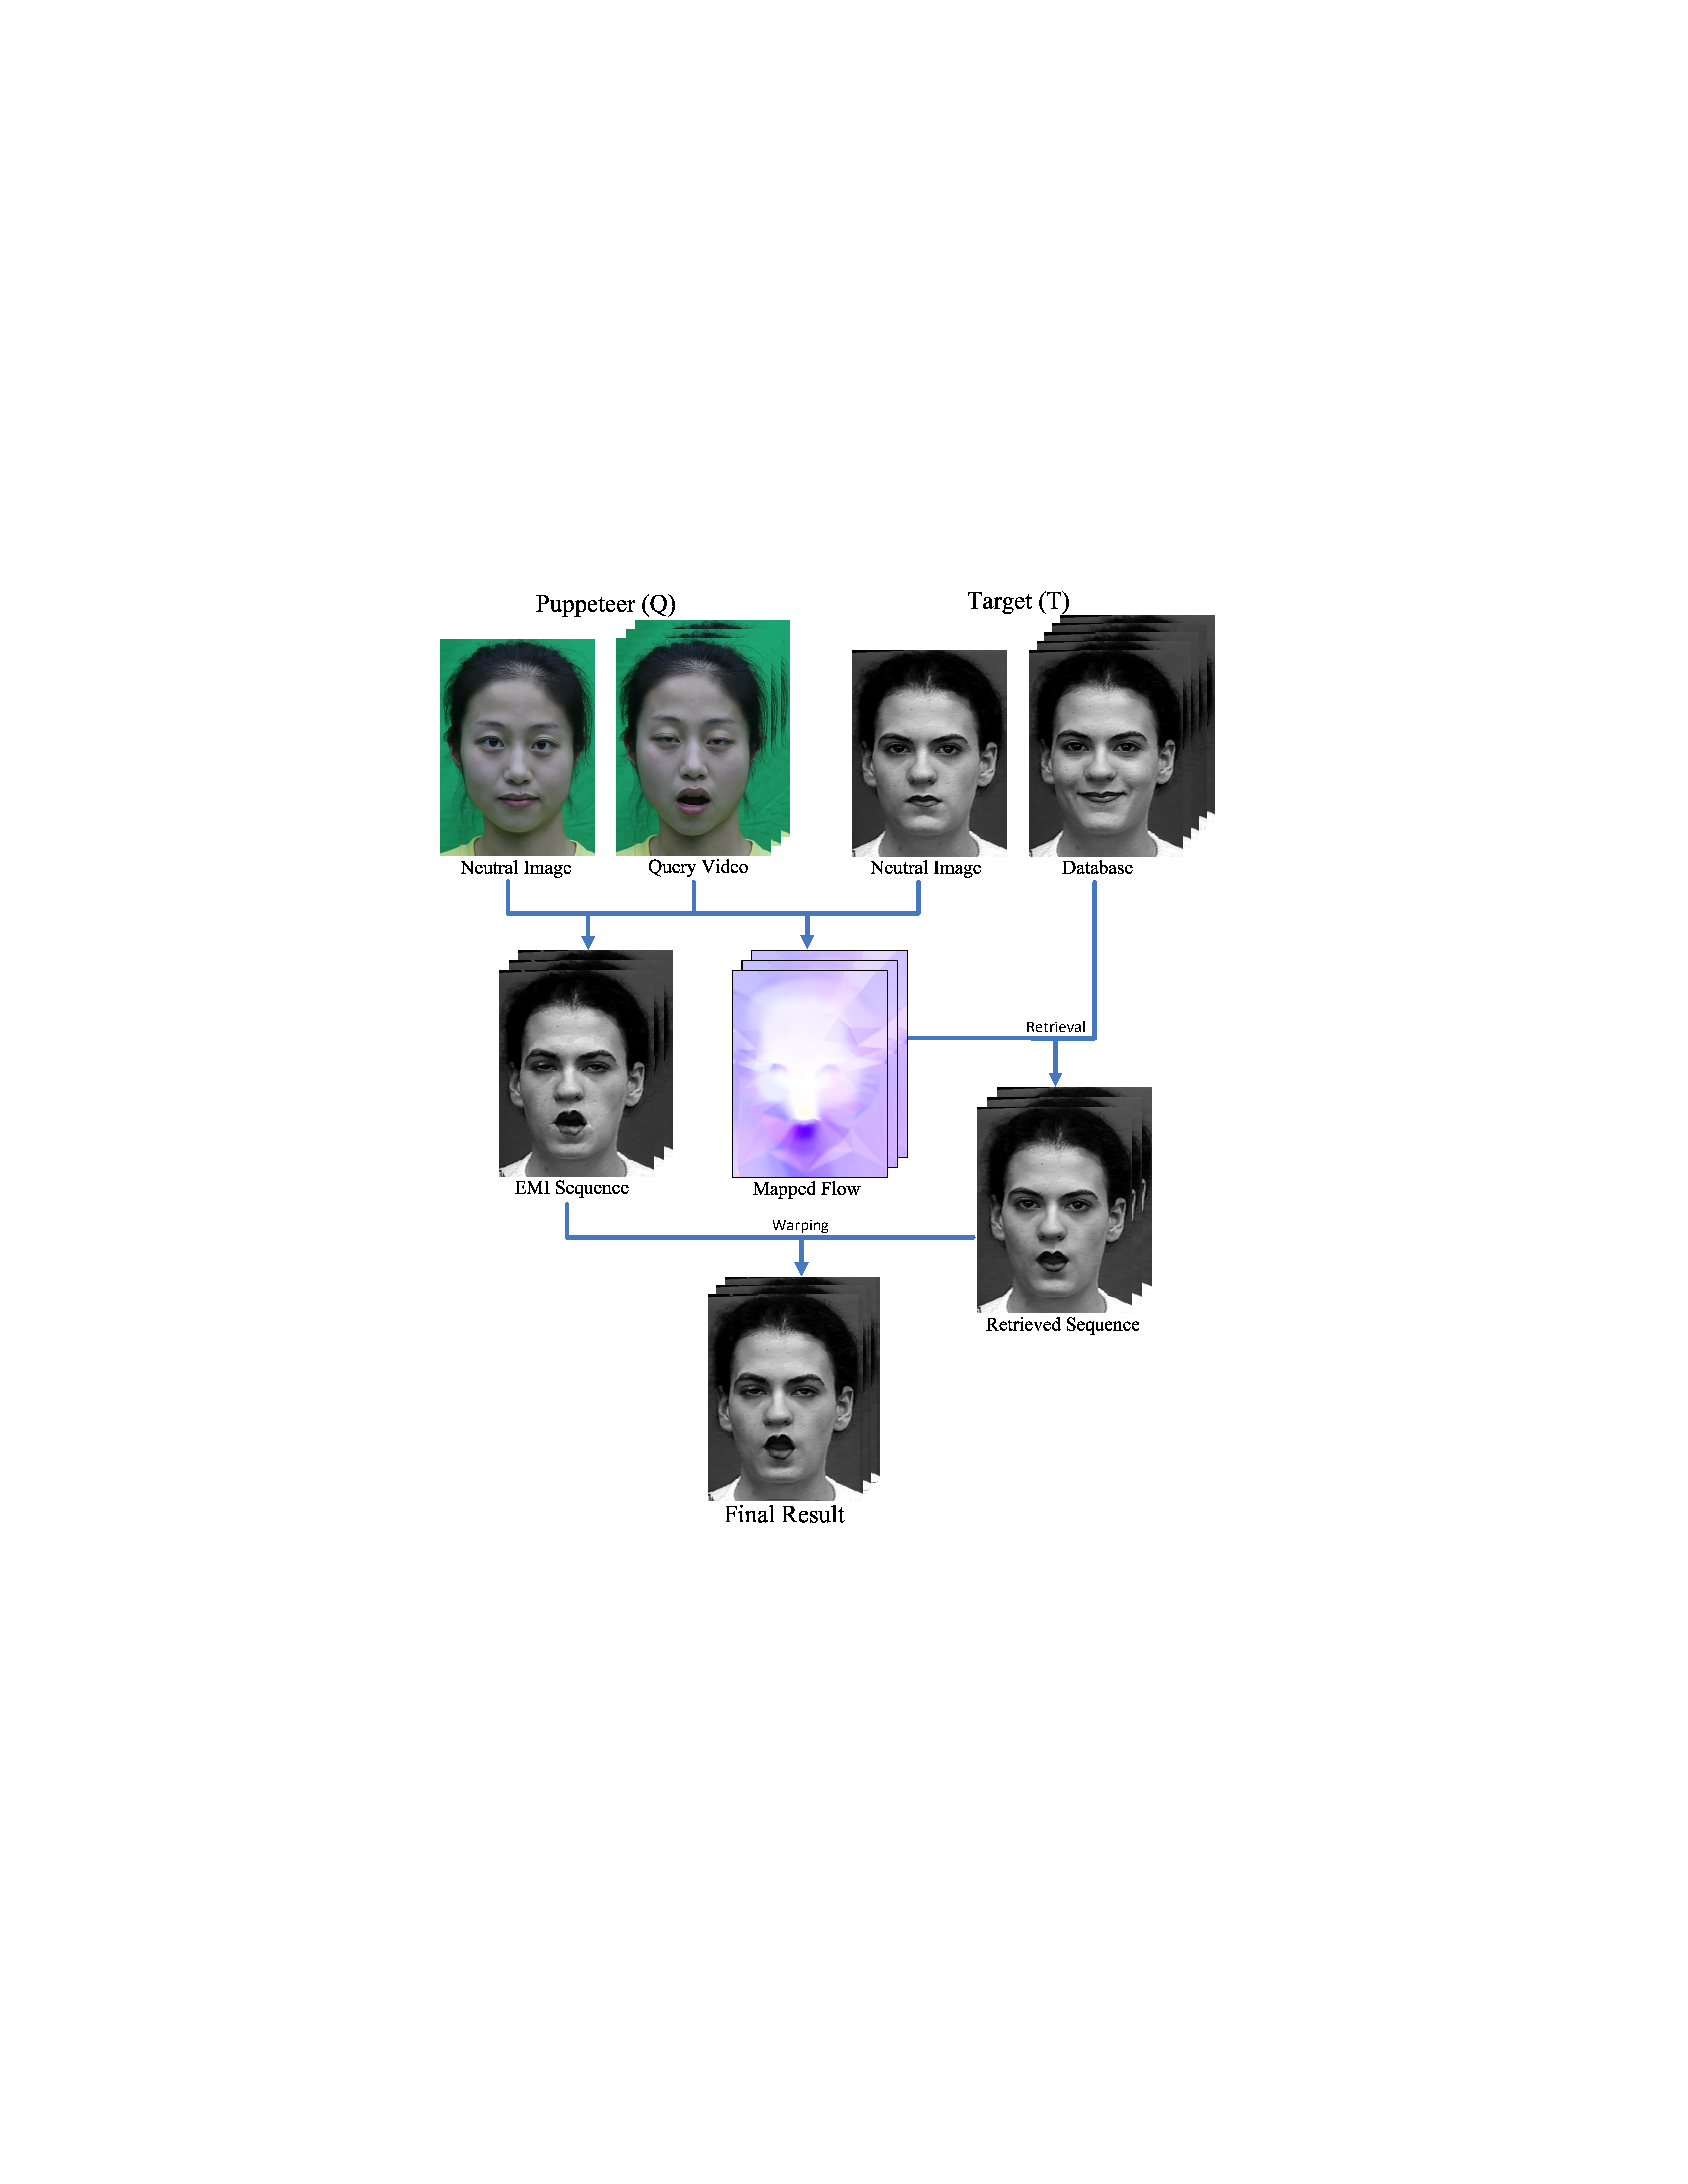
\includegraphics[width=0.95\textwidth]{data/img/overview.pdf}
    \caption{系统概览. 首先将每个查询帧和它的中性面部之间的光溜映射到目标人,用来从数据库中检索。同时,目标人的中性图像被扭曲以生成含有查询表情的EMI序列。最后,检索序列用EMI 精炼,来生成最终结果。}
    \label{fig:overview}
\end{figure}
图~\ref{fig:overview}展示了我们系统的概况。要为目标人生成逼真的表情,我们首先捕捉一段这个人展示基本表情的视频,比如生气、恐惧、惊奇、伤心、高兴、厌恶。有了另一个我们叫做人偶师(puppeteer)的人的面部表情,我们的方法尝试利用目标人的数据合成同样的表情。

具体而言,对于每个输入帧,我们使用第~\ref{sec:metric}章描述的基于光流相似度度量方法查询数据库获得$k$个与输入帧有最相近表情的目标人的视频帧。正如在第~\ref{sec:retrieval} 章描述的那样,我们把这个任务认为是和最短路问题一样找最优连续帧,而不是像Kemelmacher-Shlizerman等人~\cite{eccv10} 直接用最相似的帧生成一个匹配序列。获得的序列包含和人偶师相似且时间一致的表情。

然而,由于数据库大小有限,为每个输入帧找到一个完美的表情匹配几乎是不可能的,更何况,一些表情的人偶师具有独特的特点。为了考虑再输入和检索帧之间细微的表情差异,我们用一个表情映射技术来生成另一个候选面部,我们称之为EMI图像,如第~\ref{sec:emi}章描述那样。EMI图片通常有比检索帧有更精确的面部表情,但她的面部外观可能有重大瑕疵。在最后一步,我们把EMI图片和检索帧结合起来从而生成有精确表情和逼真外观的最终输出帧,如第~\ref{sec:emi}章所述。
\section{算法}
\subsection{表情相似度度量}\label{sec:metric}
给出人偶师的面部图片$Q_e$, 我们的系统试图从目标人的数据库中找到对应面部图片$T_e$,这幅图片有和$Q_e$最接近的面部表情. 为此我们需要能准确测量$Q_e$ 和 $T_e$之间表情差异的面部相似度度量, 同时忽视两幅图片的外表差异。

为了找到这样一个度量,我们的系统使用人偶师和目标人的中性面,分别记作$Q_n$ 和 $T_n$。当我们建立数据库的时候 $T_n$ 只需要标识一次,我们假设 $Q_n$ 在输入视频中由用户标记。为了说明人偶师的面部如何从 $Q_n$ 到 $Q_e$变化,我们能计算两幅图片中的光流场~\cite{celiu}记作 \mbox{\boldmath $F$}$_{Q_n \to Q_e}\in\mathbb{R}^{m \times 2}$, 这里$m$表示$Q_n$中的所有人脸像素。为了从光场中去除全局头部运动,我们用不随表情变化的鼻子区域来估计2D相似度变化,在计算表情差异前先把$Q_e$和$Q_n$对齐。我们也用脸的宽度归一化光流。类似的,$T_n$和$T_e$之间的光流场\mbox{\boldmath $F$}$_{T_n \to T_e}\in\mathbb{R}^{n \times 2}$, 其中$n \neq m$, 也可以计算。然而,由于身份/外观不同我们不能直接对比这两个光场。
\begin{figure}[htbp]
\centering
    \subcaptionbox{面部标记}{
    \label{fig:face_marker}
    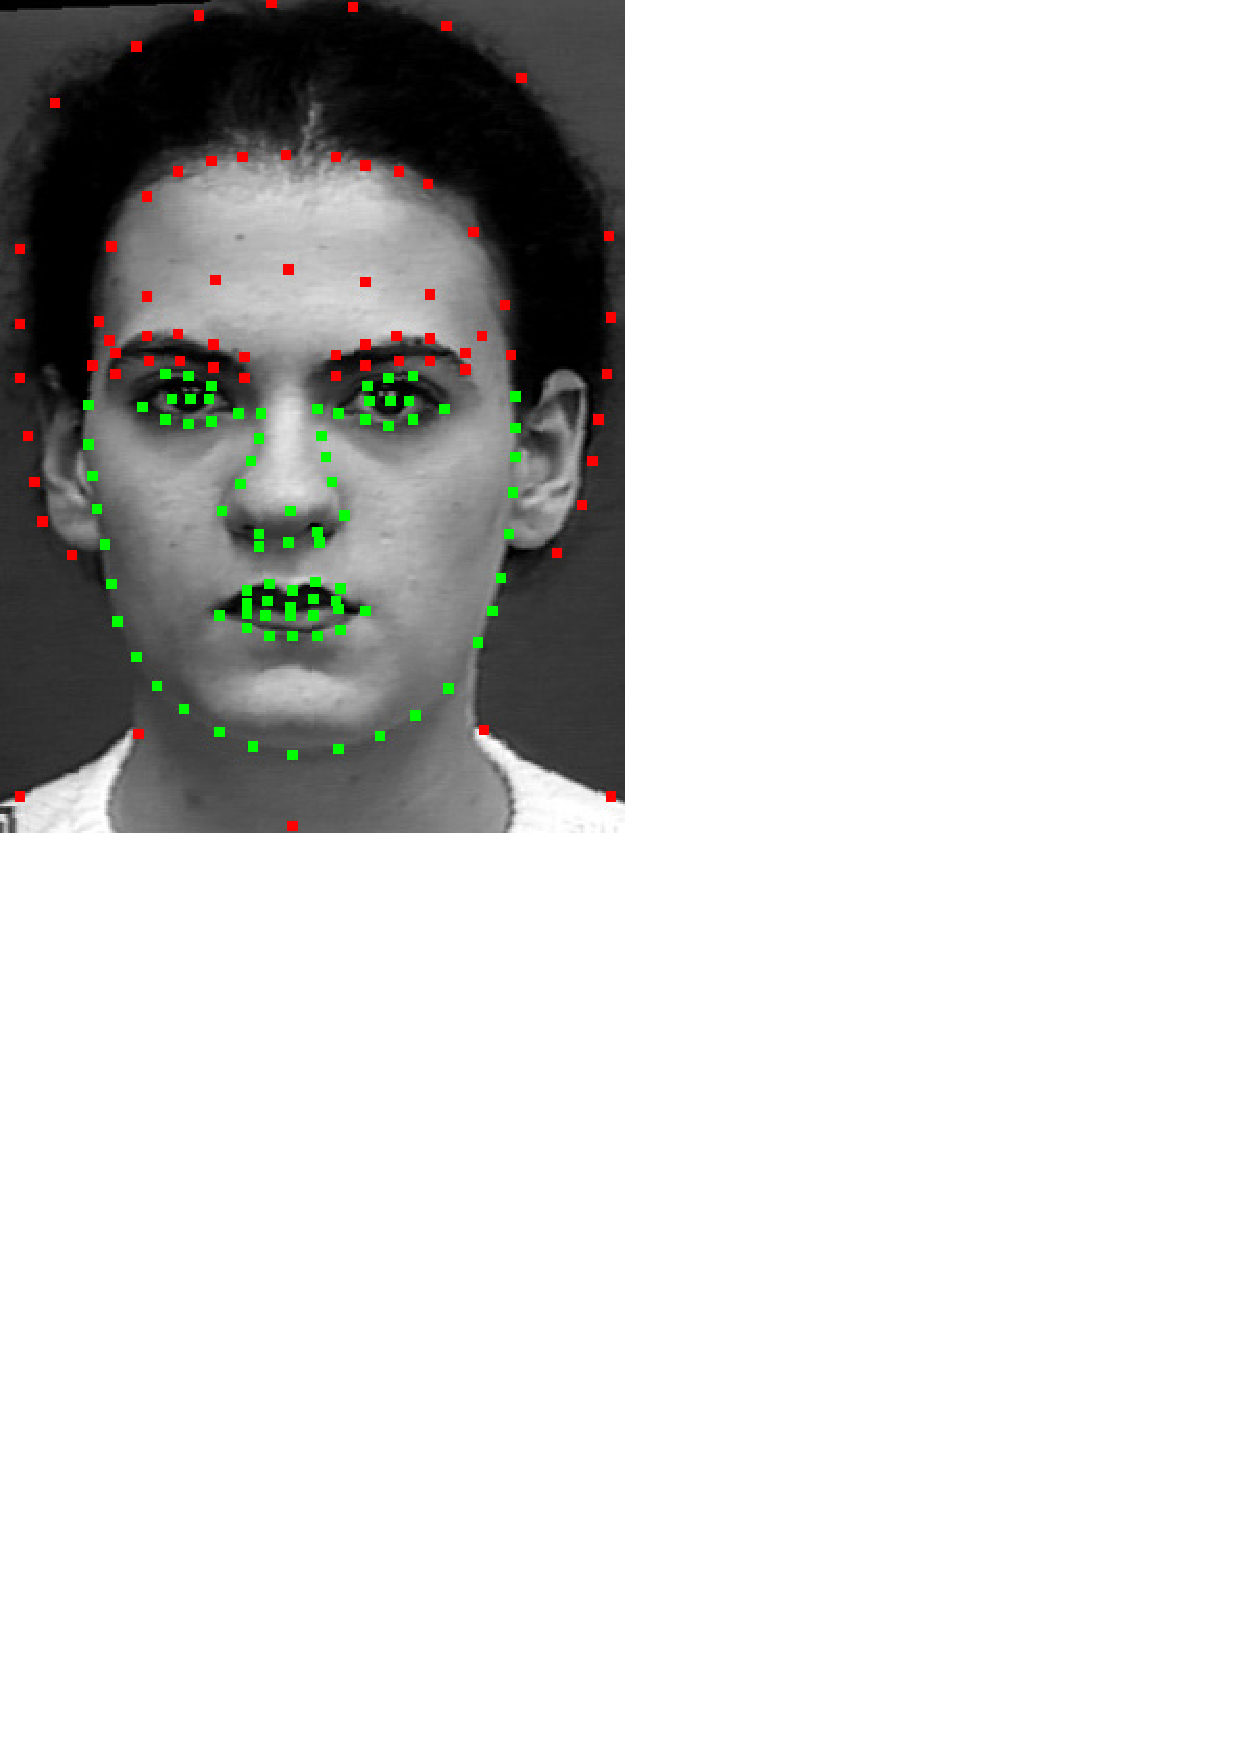
\includegraphics[width=0.20\textwidth]{data/img/facemarker.pdf}}
    \hspace{5mm}
    \subcaptionbox{局部区域}{
    \label{fig:face_region}
    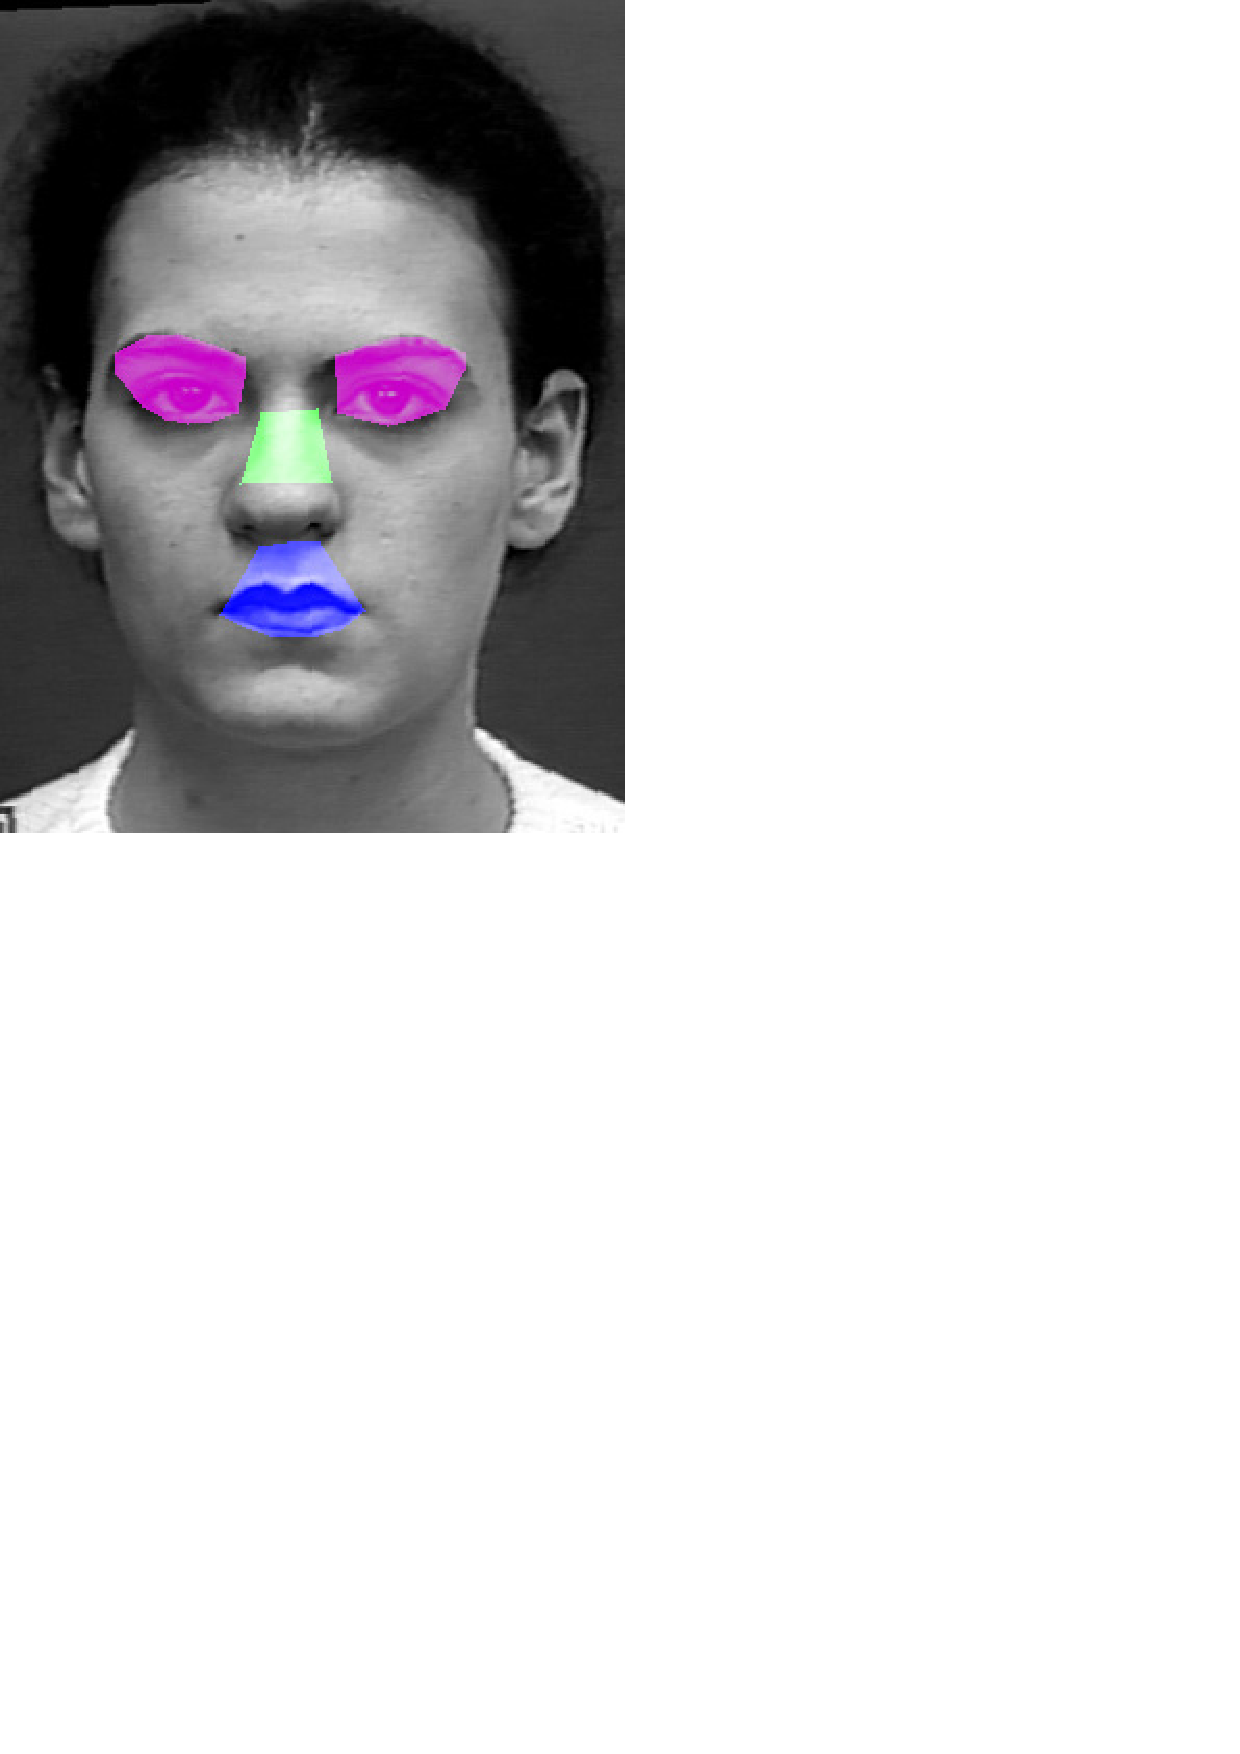
\includegraphics[width=0.20\textwidth]{data/img/faceregion.pdf}}
    \caption{中性脸初始化 (a) 绿色是ASM的标记,红色是手工标记
    (b) 眼睛、嘴巴、鼻子区域分别用品红、蓝色、绿色标记。}
    \label{fig:face}
\end{figure}
为了在两个光场之间建立精确的对应,我们首先使用Active Shape Model (ASM)~\cite{asm}只检测在中性面$Q_n$和$T_n$的面部标志物,该方法对于中性表情的正面人脸很有效。然而它无法覆盖我们算法在之后几步中需要的所有面部。因此我们在两个中性面上手工标注标志点,如图~\ref{fig:face_marker}所示。然后我们用Delauney三角网标出$Q_n$ 和 $T_n$ 中的脸部区域,这引出一个只能像素注册函数$g: Q_n \to T_n$。此外,由于两个身份之间的语义对应应该对不同的面部表情具有不变性,可以合理假设$g': Q_e \to T_e$两个表情图片的注册函数近似和$g: Q_n \to T_n$ 相同。有了注册函数,对于一个点$\vec{a}\in Q_n$转移到$\vec{a}' \in Q_e$,它在$T_n$对应的光流向量按如下计算:
\begin{equation}\label{eq:map2}
\Delta \vec{b}=g(\vec{a}')-g(\vec{a}),
\end{equation}
其中$\vec{b}=g(\vec{a})$是$T_n$上$\vec{a}$的对应点。

通过在$Q_n$上的所有面部像素应用这个映射,我们获取了一种映射好的光流场\mbox{\boldmath $F$}$'_{Q_n \to Q_e}$,可以通过与\mbox{\boldmath $F$}$'_{Q_n \to Q_e}$对比测量两个表情有多接近。以往工作指出~\cite{eccv10},表情差异的主要来源是眼睛和嘴巴区域,因此我们只用这些区域的像素来计算表情相似度(参见图~\ref{fig:face_region})。直接的方法是通过绝对的光流差计算$Q_e$ 和 $T_e$之间的表情差异:
\setlength\arraycolsep{1pt}
\begin{eqnarray}\label{eq:dist_mag}
d_e(Q_e, T_e)&=& \alpha_{e}\sum_{i\in\text{eye}}\left\|F'_{Q_n \to Q_e,i} -F_{T_n \to T_e,i}\right\| \nonumber\\
  &&+\alpha_{m}\sum_{i\in\text{mouth}}\left\|F'_{Q_n \to Q_e, i} -F_{T_n \to T_e, i}\right\|,
\end{eqnarray}

这里下标$i$表示光流矩阵\mbox{\boldmath $F$}中第$i$行。$\alpha_{\{e, m\}}$分别是眼睛和嘴巴区域的权重。
\begin{figure}[htbp]
\centering
    \subcaptionbox{}{
    \label{fig:metric_driven}
    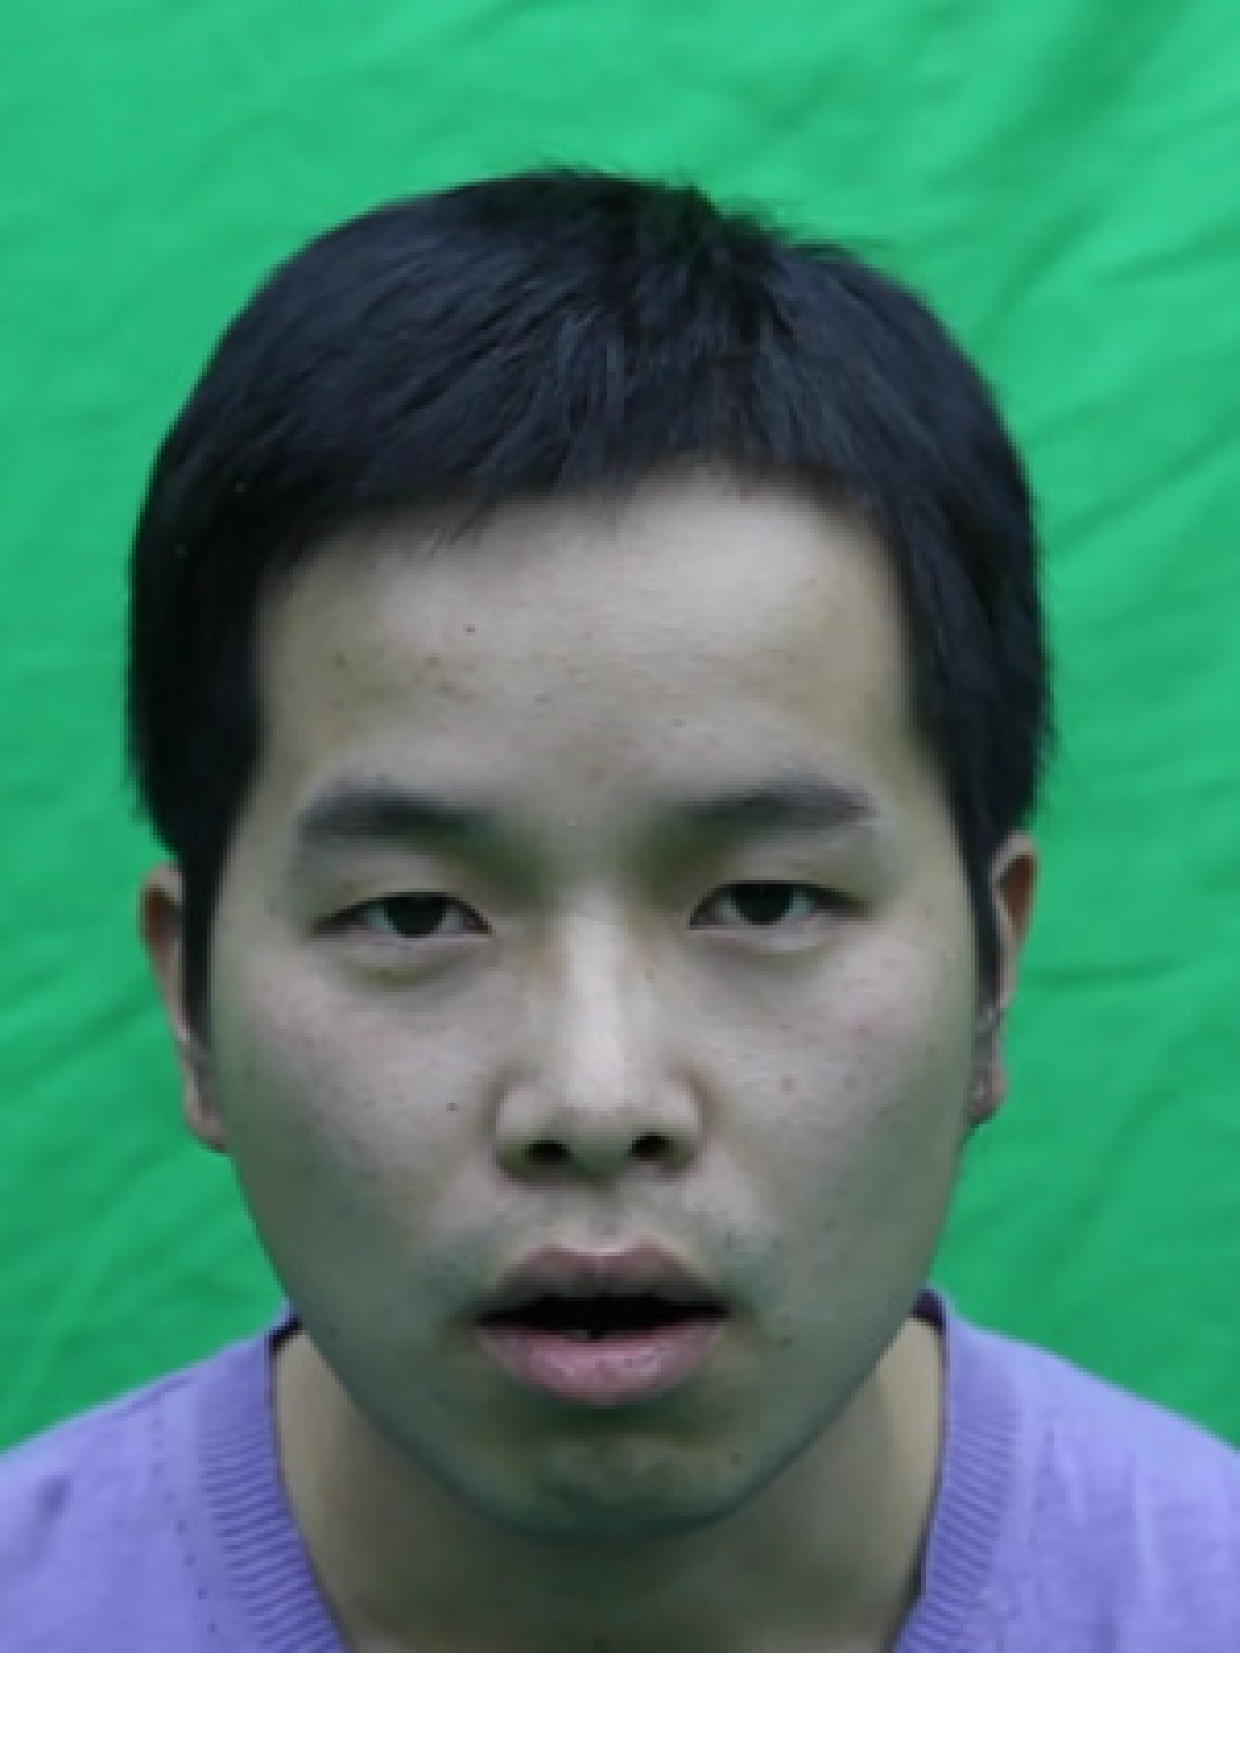
\includegraphics[width=0.2\textwidth]{data/img/metric_likai_0380_00103.pdf}}
    \subcaptionbox{}{
    \label{fig:metric_lbp}
    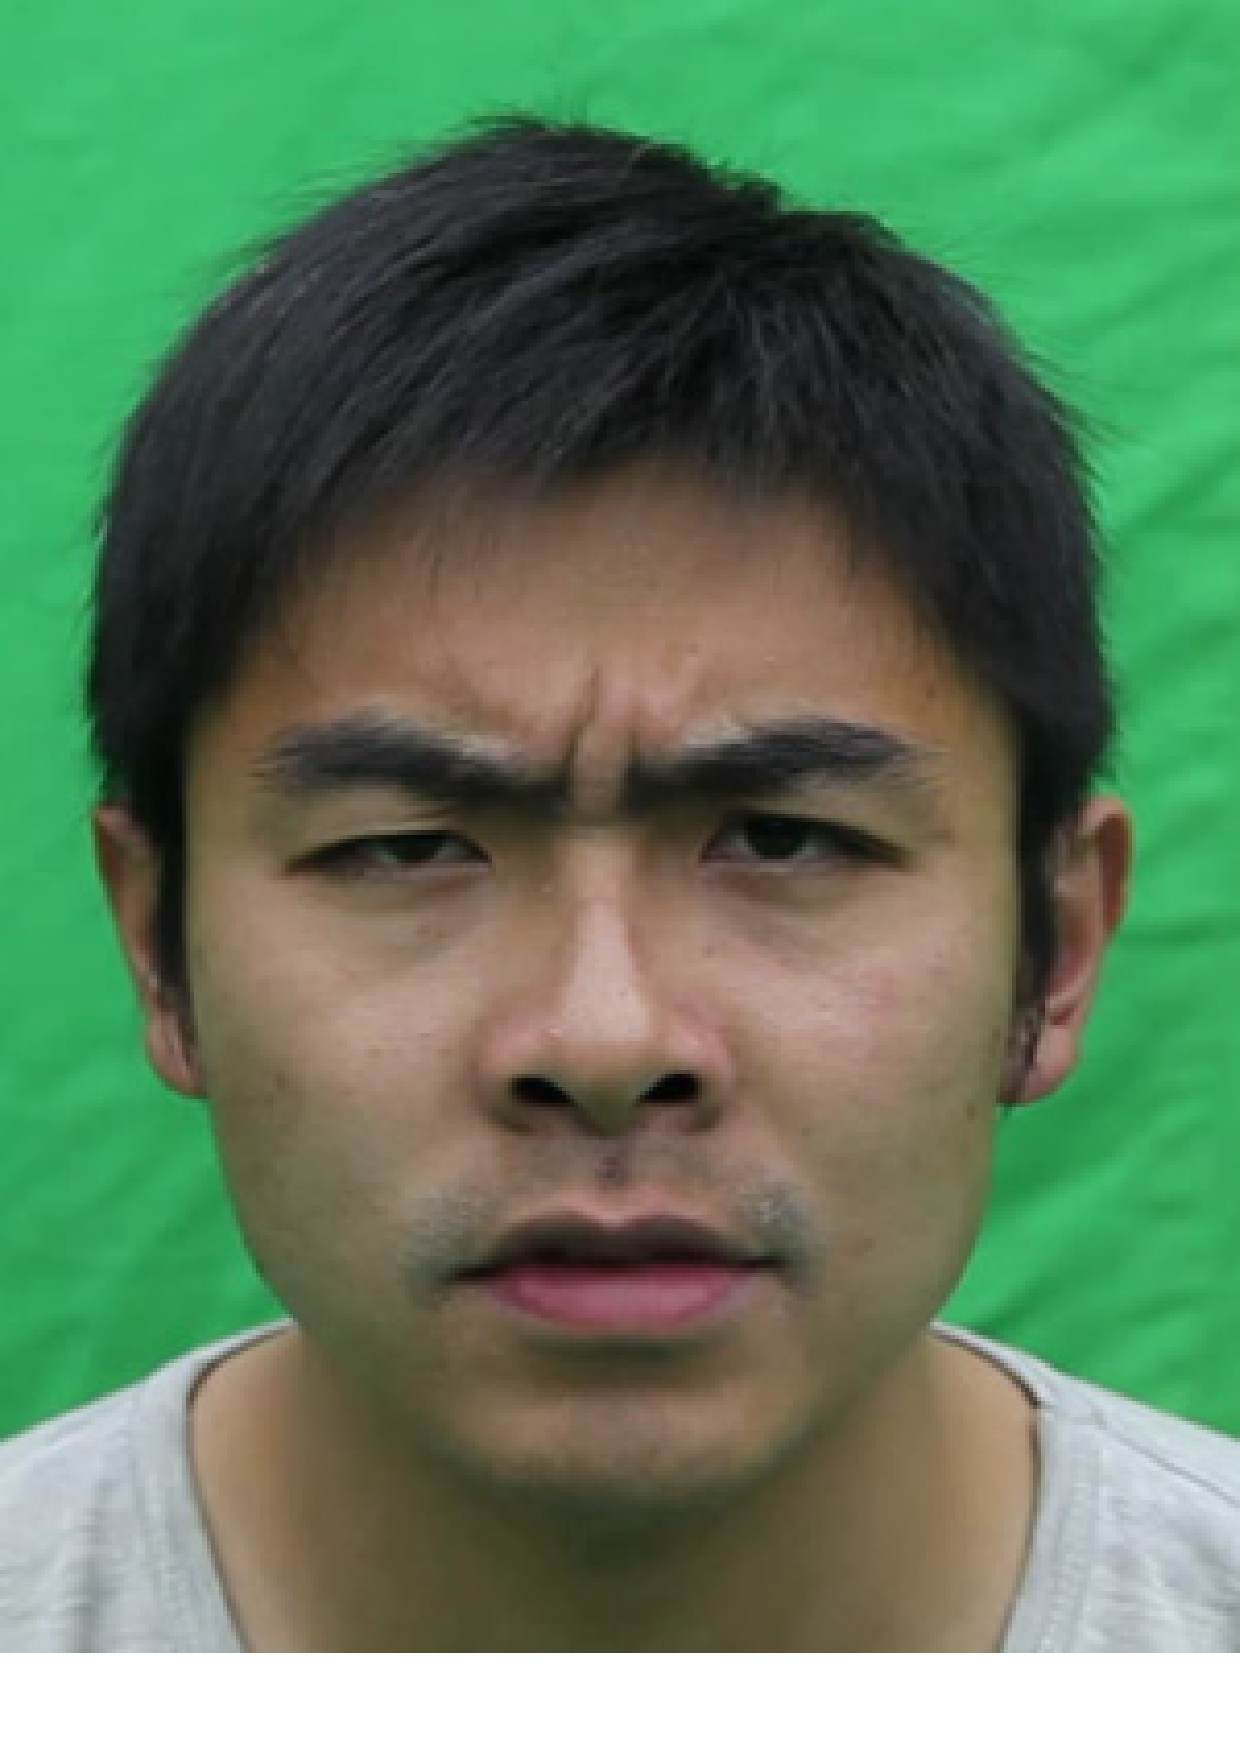
\includegraphics[width=0.2\textwidth]{data/img/metric_lbp_00102.pdf}}
    \subcaptionbox{}{
    \label{fig:metric_mag}
    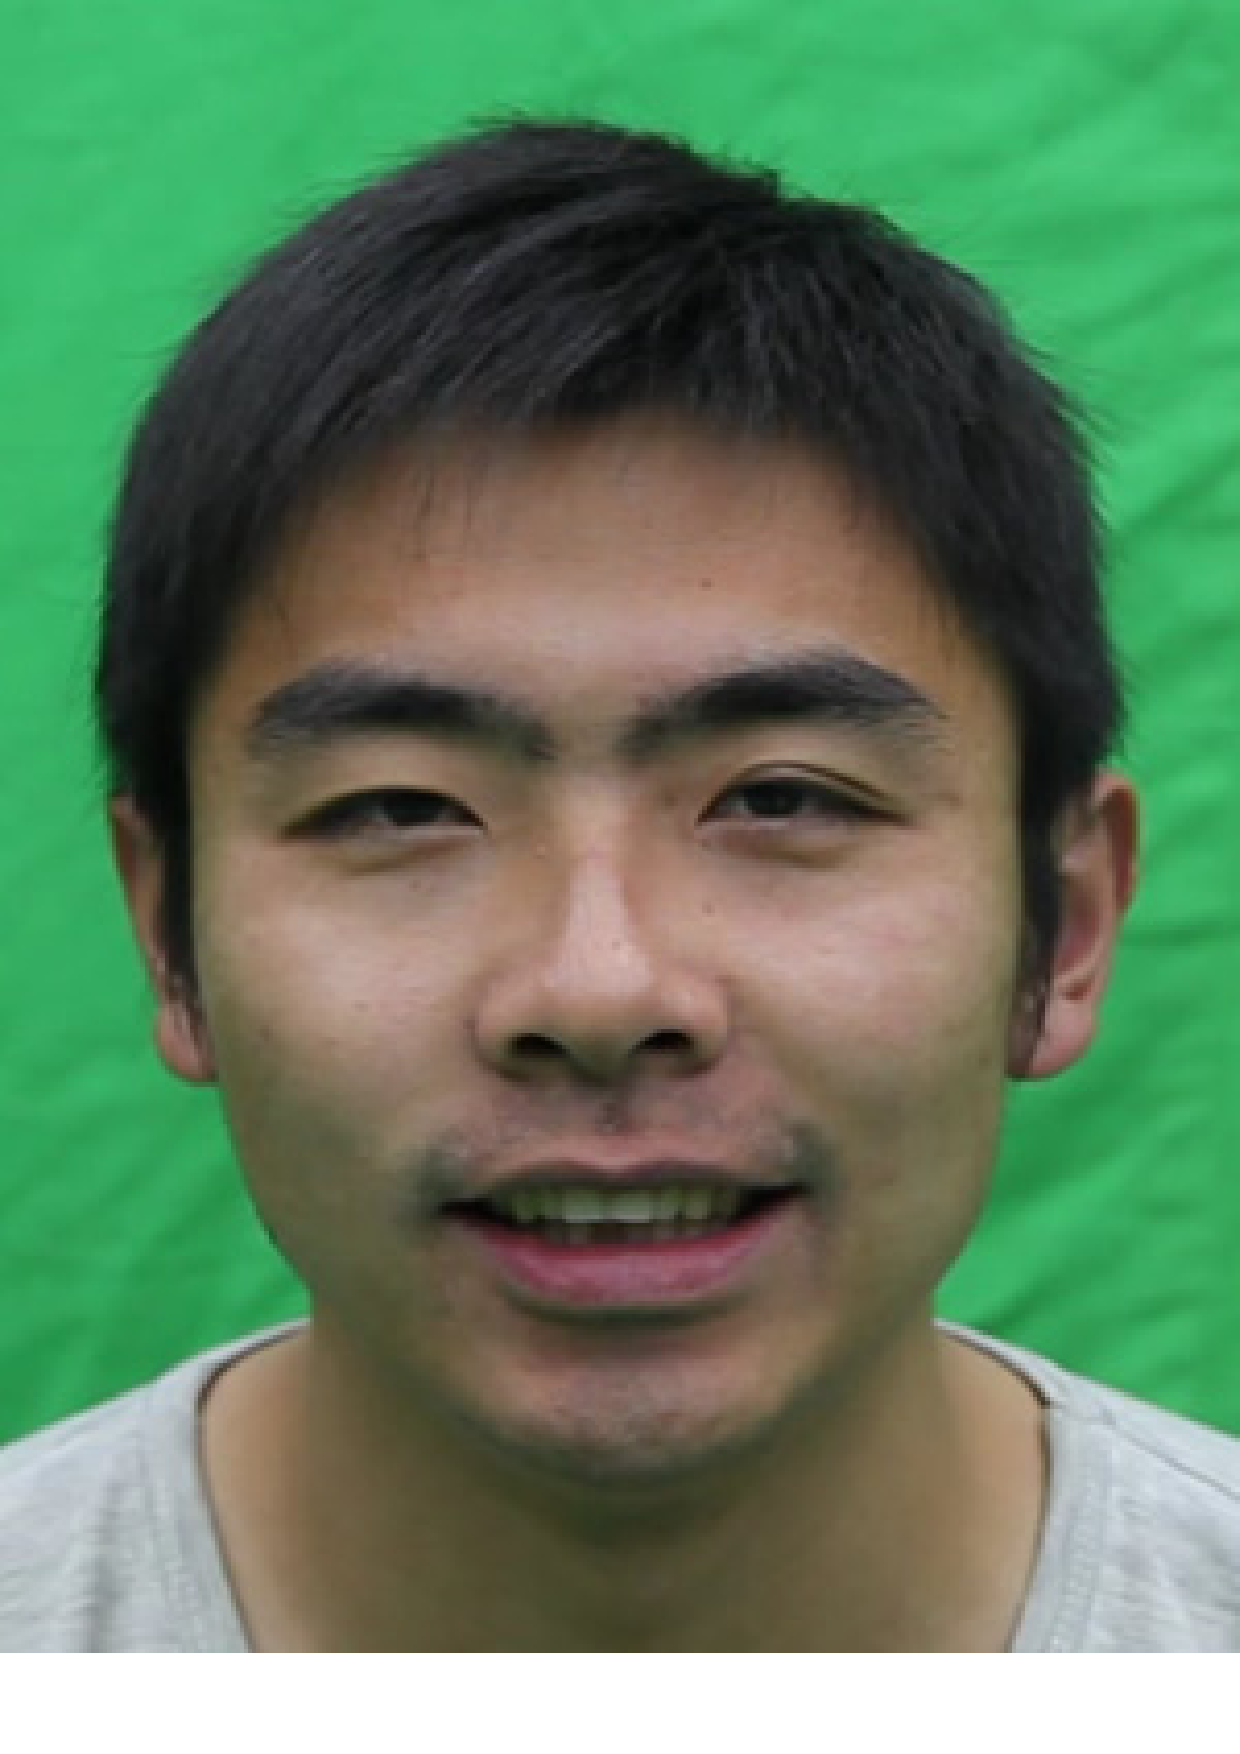
\includegraphics[width=0.2\textwidth]{data/img/metric_OFmag_00102.pdf}}
    \subcaptionbox{}{
    \label{fig:metric_magori}
    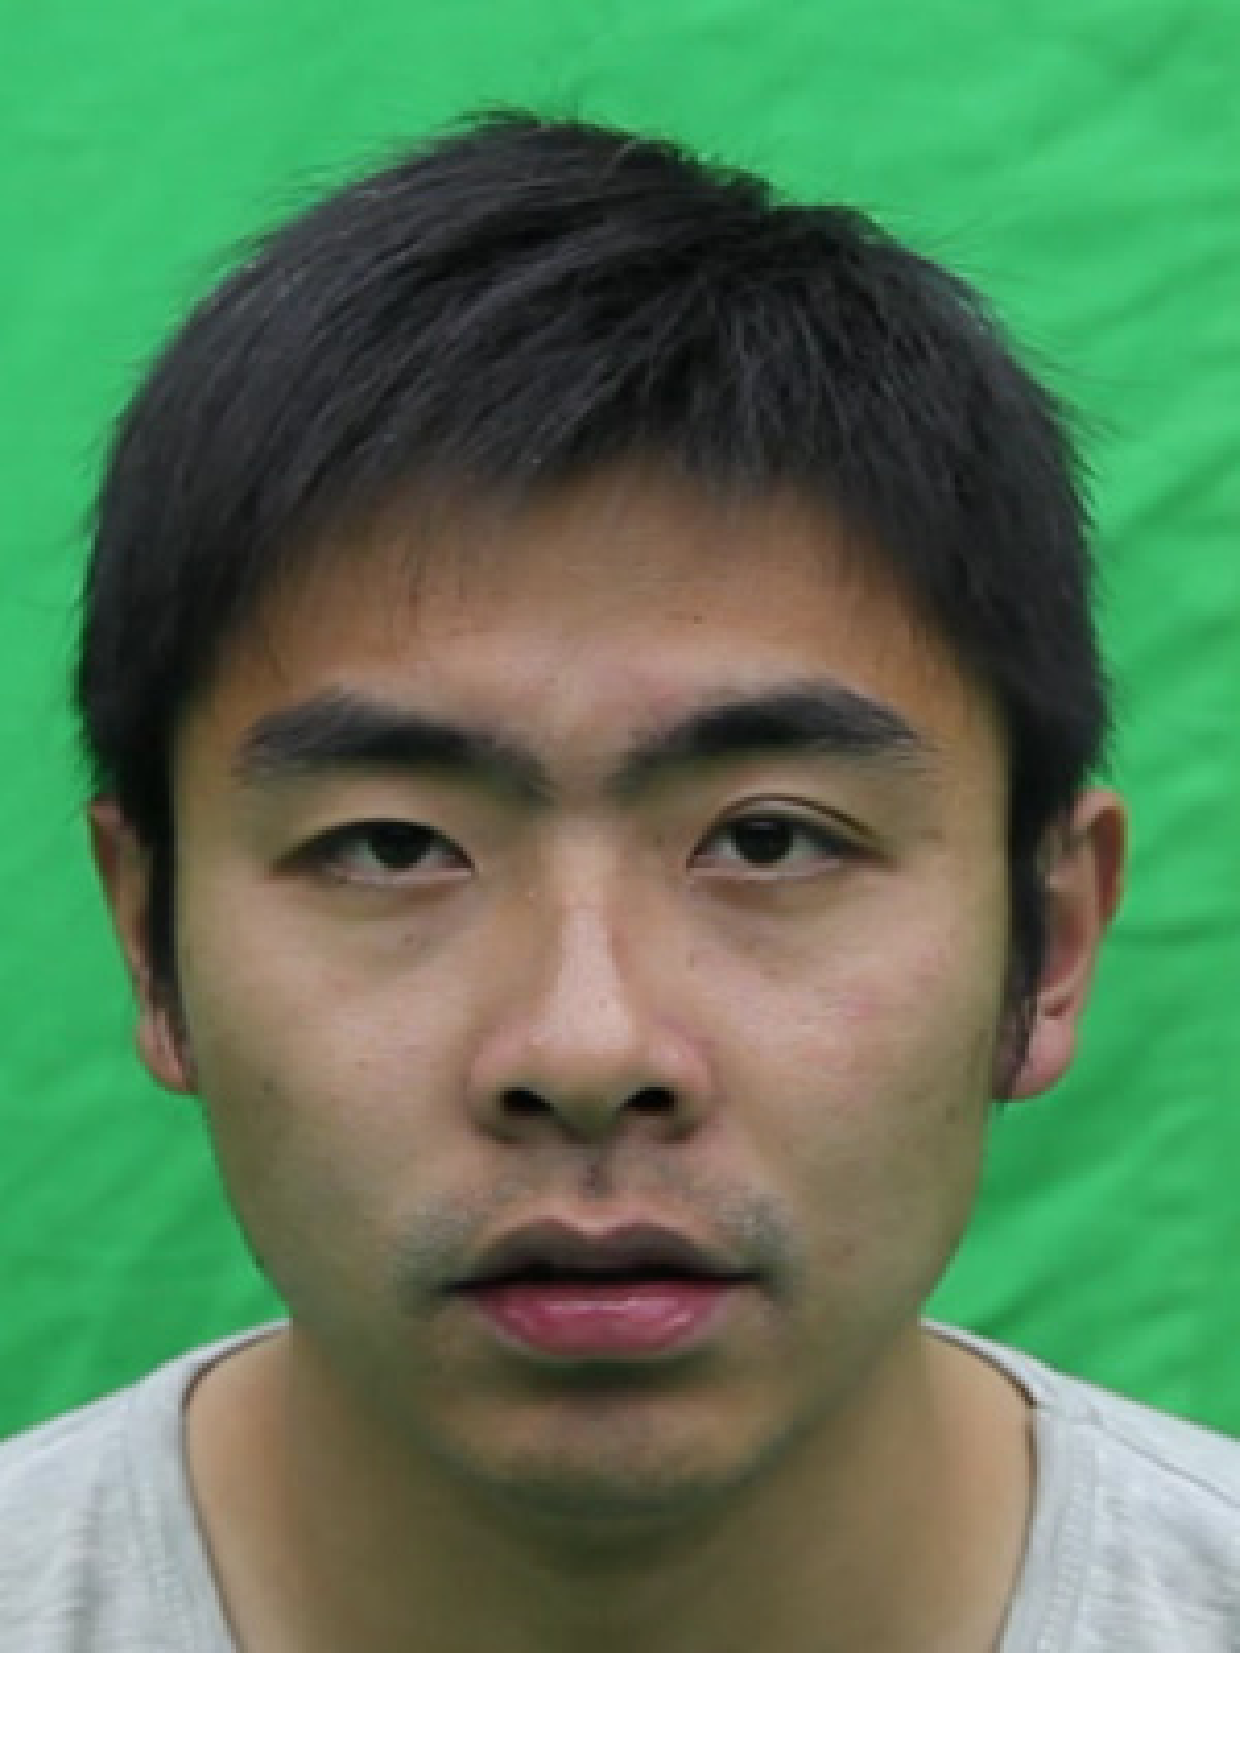
\includegraphics[width=0.2\textwidth]{data/img/metric_OFmagori_00102.pdf}}
    \caption{表情度量对比。 (a) 查询帧。 (b) 由LBP方法得到的最相似表情,它有一个不理想的皱眉。 (c) 由等式~\ref{eq:dist_mag}获得的最相似表情,有一个笑容而不是惊奇。 (d) 由等式~\ref{eq:dist_comb}获得的最相似表情,和查询帧匹配很好}
    \label{fig:metric}
\end{figure}

等式~\ref{eq:dist_mag}中的距离度量在我们大多数实验中都很成功,但我们发现会偶尔产生如图~\ref{fig:metric}所示的错误。这是因为在等式~\ref{eq:dist_mag}中,我们仅考虑了\mbox{\boldmath $F$}$'_{Q_n \to Q_e}-$\mbox{\boldmath $F$}$_{T_n \to T_e}$的光流差异的大小。但光流的方向通常包含更多有关表情的重要信息。比如笑脸通常与嘴角的上翘相关,而哭脸和嘴角下弯相关。这表明在$Q_e$中的表情与$T_e$中的很不一样,如果\mbox{\boldmath $F$}$'_{Q_n \to Q_e}$到\mbox{\boldmath $F$}$_{T_n \to T_e}$的差异方向很不一样,即便差异大小很小。有了这个发现,我们重新设计表情距离度量如下:
\setlength\arraycolsep{1pt}
\begin{eqnarray}
d_b(\vec{u},\vec{v})&=&\beta_m|\vec{u}-\vec{v}|+\beta_o(-\vec{u}\cdot\vec{v}+|\vec{u}||\vec{v}|), \label{eq:d0}\\
d_e(Q_e, T_e)&=&\alpha_{e}\sum_{i\in\text{eye}}d_b(F'_{Q_n \to Q_e,i}, F_{T_n \to T_e,i})\nonumber\\
           &&+\alpha_{m}\sum_{i\in\text{mouth}}d_b(F'_{Q_n \to Q_e, i}, F_{T_n \to T_e, i}),\label{eq:dist_comb}
\end{eqnarray}

这里$\beta_{\{m, o\}}\in[0,1]$分别是大小和方向的权重,且$\beta_m+\beta_o=1$。 当$\beta_o$ 等于零,等式~\ref{eq:dist_comb}简化为等式~\ref{eq:dist_mag}。在等式~\ref{eq:d0} 中的偏移量$|\vec{u}||\vec{v}|$确保方向项非负。注意此距离度量不保证对称性和三角不等式。为使之更有数学味,可以计算反向距离$d_e(T_e,Q_e)$,用二者平均值作为最终距离度量。但实际上我们发现这并无必要,因为$d_e(Q_e, T_e)$已很好描述不同身份两张图片的表情差异,对我们的应用而言已足够。
\subsection{基于检索的视频合成}\label{sec:retrieval}
使用如上定义的相似性度量,一个视频合成的简单方法是为每个输入帧,找到其在数据库中的最近邻表清,并叠在一起,以形成最终的输出视频。然而,我们发现这种方法并不很好,在最终视频中面部表情的时间相干性没有得到很好的保持,并且最终的视频经常出现抖动。补充材料包含了说明此问题的视频。我们的系统采用了一些额外的技术来解决的时间一致性问题,我们将在本小节详细介绍。
\subsubsection{结合表情速度}
首先,在公式~\ref{eq:dist_comb}中定义的距离度量只考虑了两个面部的表情相似度。然而在视频中,我们需要关心在每一帧表情变化的速度。最相似的帧应该是表情及其变化速度都与查询帧相符的。为了保证表情速度,我们在视频序列中简单地计算另一个在当前帧和下一帧之间的光流。记$Q_e^{(q)}$为第 $q$个查询帧,表情速度计算如下:
\begin{equation}\label{eq:dF_Q}
\text{d} \mbox{\boldmath $F$}_{Q_e^{(q)}} = \mbox{\boldmath $F$}_{Q_e^{(q)}\to Q_e^{(q+1)}}.
\end{equation}

类似的,对于在数据库中的帧$T_e^{(t)}$,我们计算表情速度为d\mbox{\boldmath $F$}$_{T_e^{(t)}}$。同样,由于$Q_e^{(q)}$ 和 $T_e^{(t)}$身份和表情差异,直接计算d\mbox{\boldmath $F$}$_{Q_e^{(q)}}$ 和 d\mbox{\boldmath $F$}$_{T_e^{(t)}}$ 距离并不好。需要扭曲表情速度光流场来去除身份差异,如我们在
第~\ref{sec:metric}章所做。我们还需要扭曲两者的速度光流场来把他们映射到中性表情,以去除他们的表情差异。

具体说,对于数据库帧,我们把\mbox{\boldmath $F$}$_{T_n\to T_e^{(t)}}$的反向光流用于 d\mbox{\boldmath $F$}$_{T_e^{(t)}}$,导出与中性表情$T_n$相符的扭曲的表情速度流d\mbox{\boldmath $F$}$'_{T_e^{(t)}}$。对于查询帧$Q_e^{(q)}$,我们把公式~\ref{eq:dist_comb} 计算的反向光流\mbox{\boldmath $F$}$'_{Q_n\to Q_e^{(q)}}$用于d\mbox{\boldmath $F$}$_{Q_e^{(q)}}$,导出与中性表情$T_n$相符的扭曲的表情速度流d\mbox{\boldmath $F$}$'_{Q_e^{(q)}}$。最后,$Q_e^{(q)}$ 和 $T_e^{(t)}$的表情速度差异计算如下:
\begin{eqnarray}\label{eq:dist_deri}
d_v(Q_e^{(q)}, T_e^{(t)})&=& \alpha_{e}\sum_{i\in\text{eye}}d_b(\text{d}F'_{Q_e^{(q)}, i}, \text{d}F'_{T_e^{(t)}, i})\nonumber\\
           &&+\alpha_{m}\sum_{i\in\text{mouth}}d_b(\text{d}F'_{Q_e^{(q)}, i}, \text{d}F'_{T_e^{(t)}, i}),
\end{eqnarray}

此处函数$d_b(\cdot,\cdot)$在公式~\ref{eq:d0}中定义。结合公式~\ref{eq:dist_comb}和公式\ref{eq:dist_deri},最终的视频表情距离度量定义如下:
\begin{equation}\label{eq:dist_all}
\mathcal{D}(Q_e^{(q)}, T_e^{(t)})=\gamma_e d_e(Q_e^{(q)}, T_e^{(t)})+ \gamma_v d_v(Q_e^{(q)}, T_e^{(t)}),
\end{equation}

这里$\gamma_{\{e,v\}}\in[0,1]$分别是表情距离和表情速度距离的权重,满足$\gamma_e+\gamma_v=1$。

图~\ref{fig:velocity}的例子表明,当表情很微妙,在度量中结合表情速度能帮助系统更好的捕捉表情变化。
\begin{figure}[htbp]
\centering
    \subcaptionbox{}{
    \label{fig:velocity_driven}
    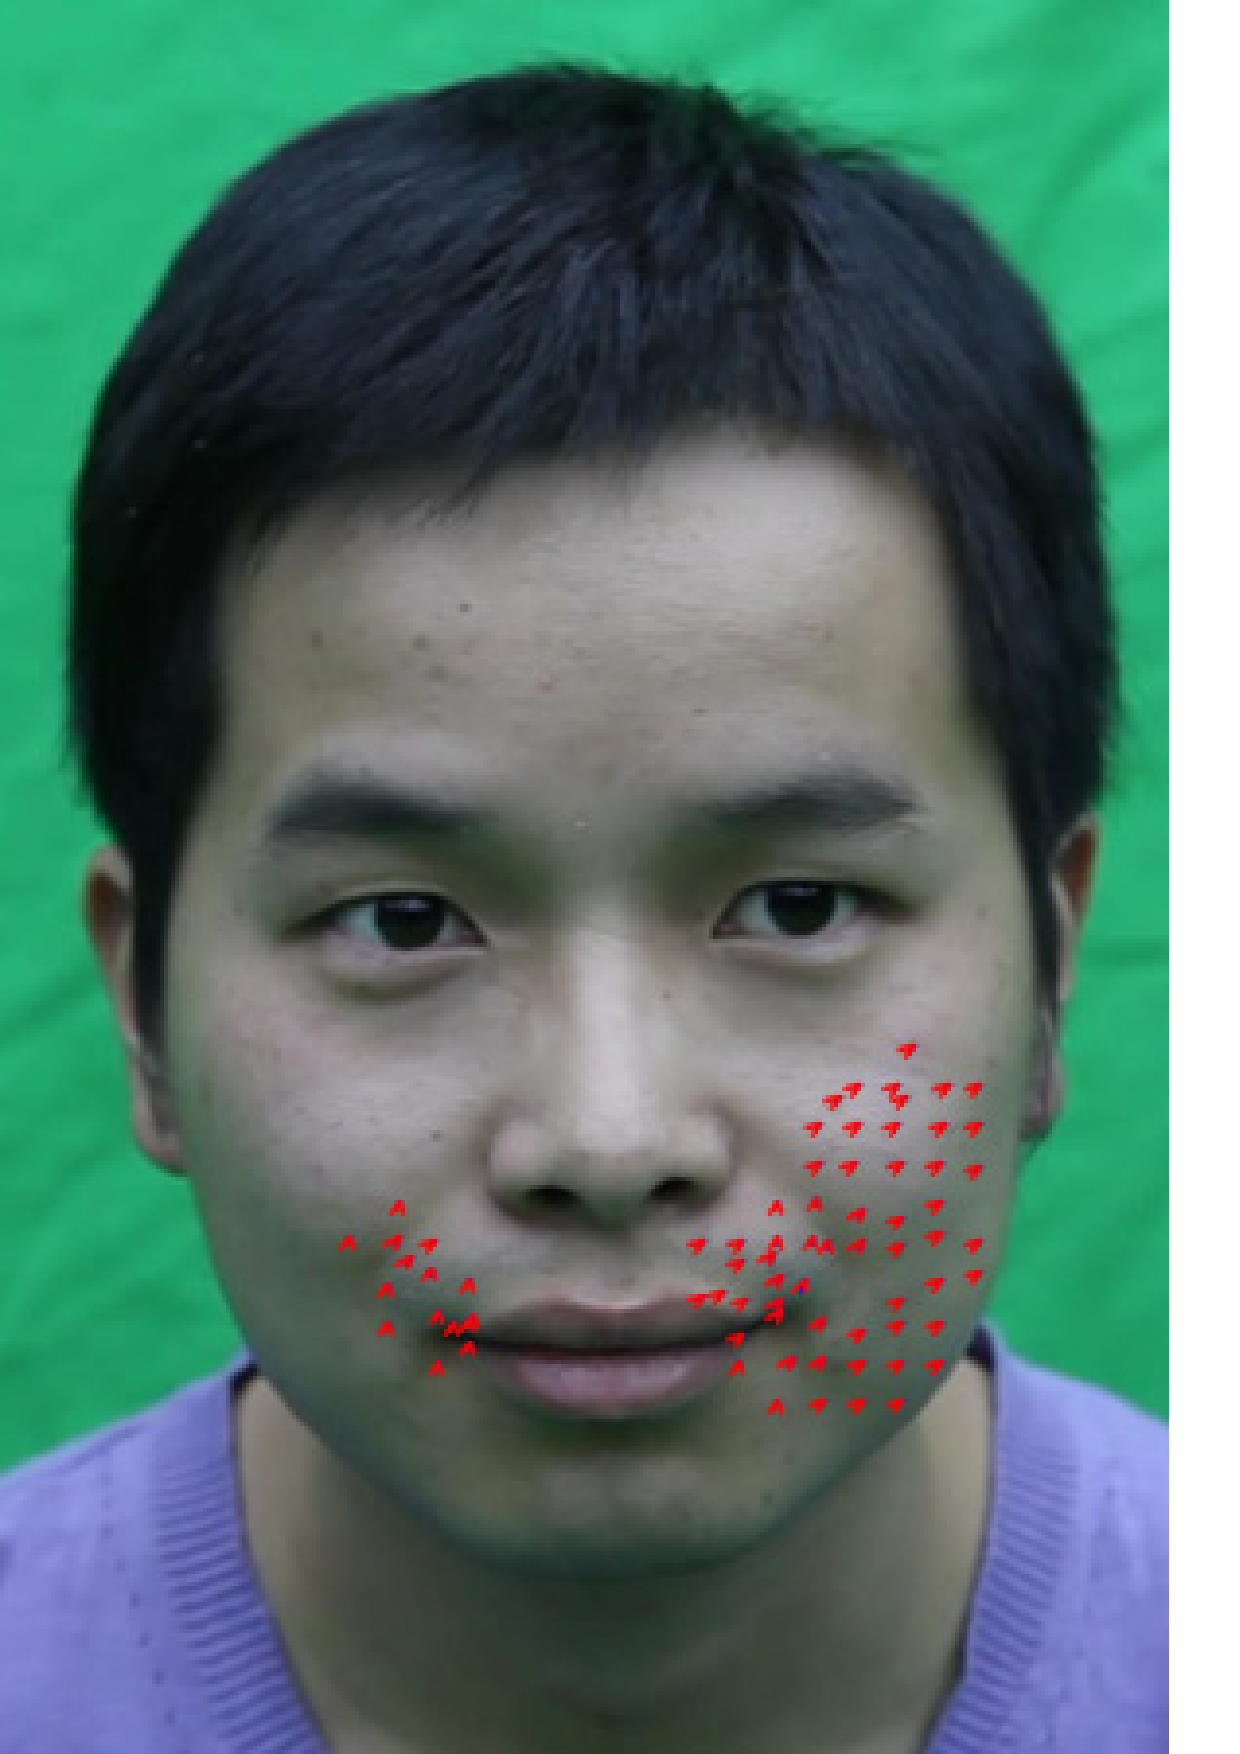
\includegraphics[width=0.205\textwidth]{data/img/velocity_likai_0380_00199_flow.pdf}}
    \subcaptionbox{}{
    \label{fig:velocity_next}
    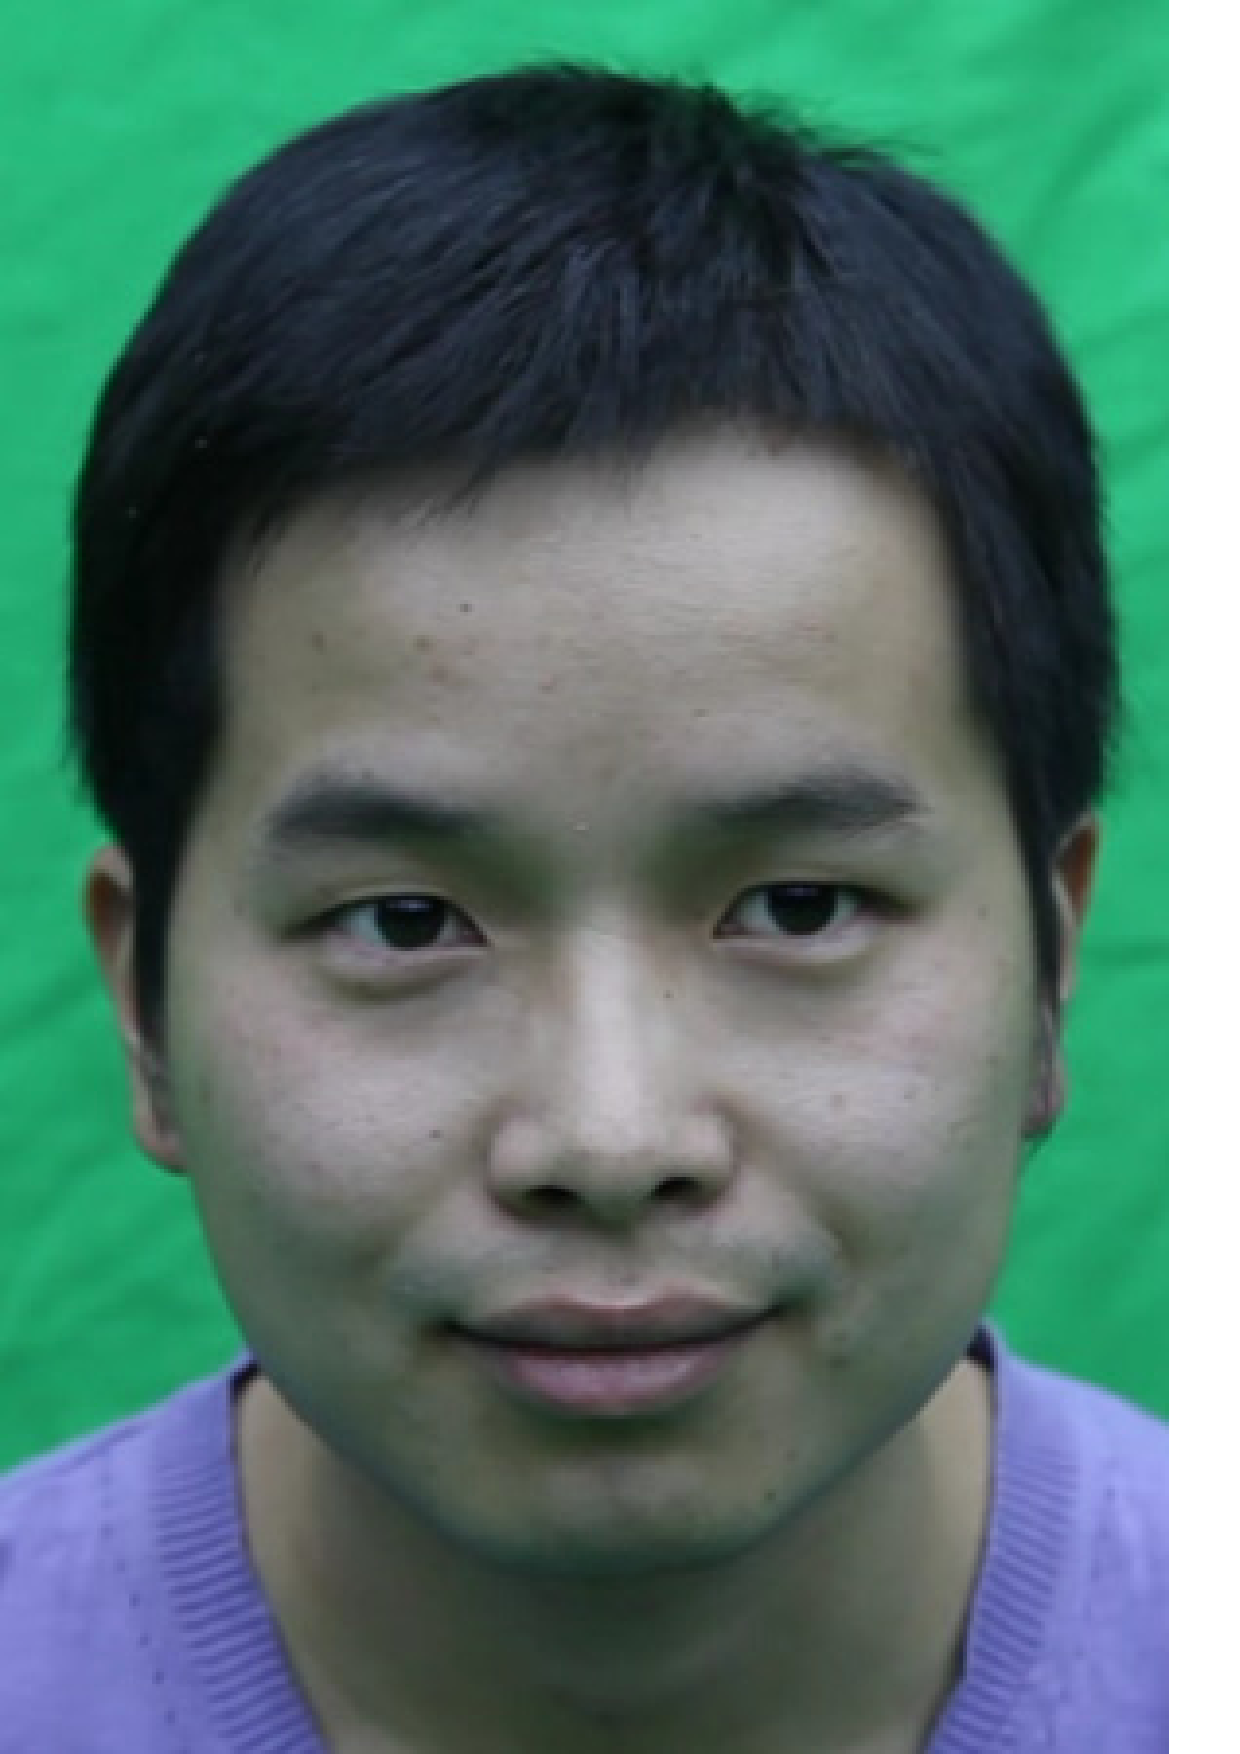
\includegraphics[width=0.205\textwidth]{data/img/velocity_likai_0380_00200.pdf}}
    \subcaptionbox{}{
    \label{fig:velocity_without}
    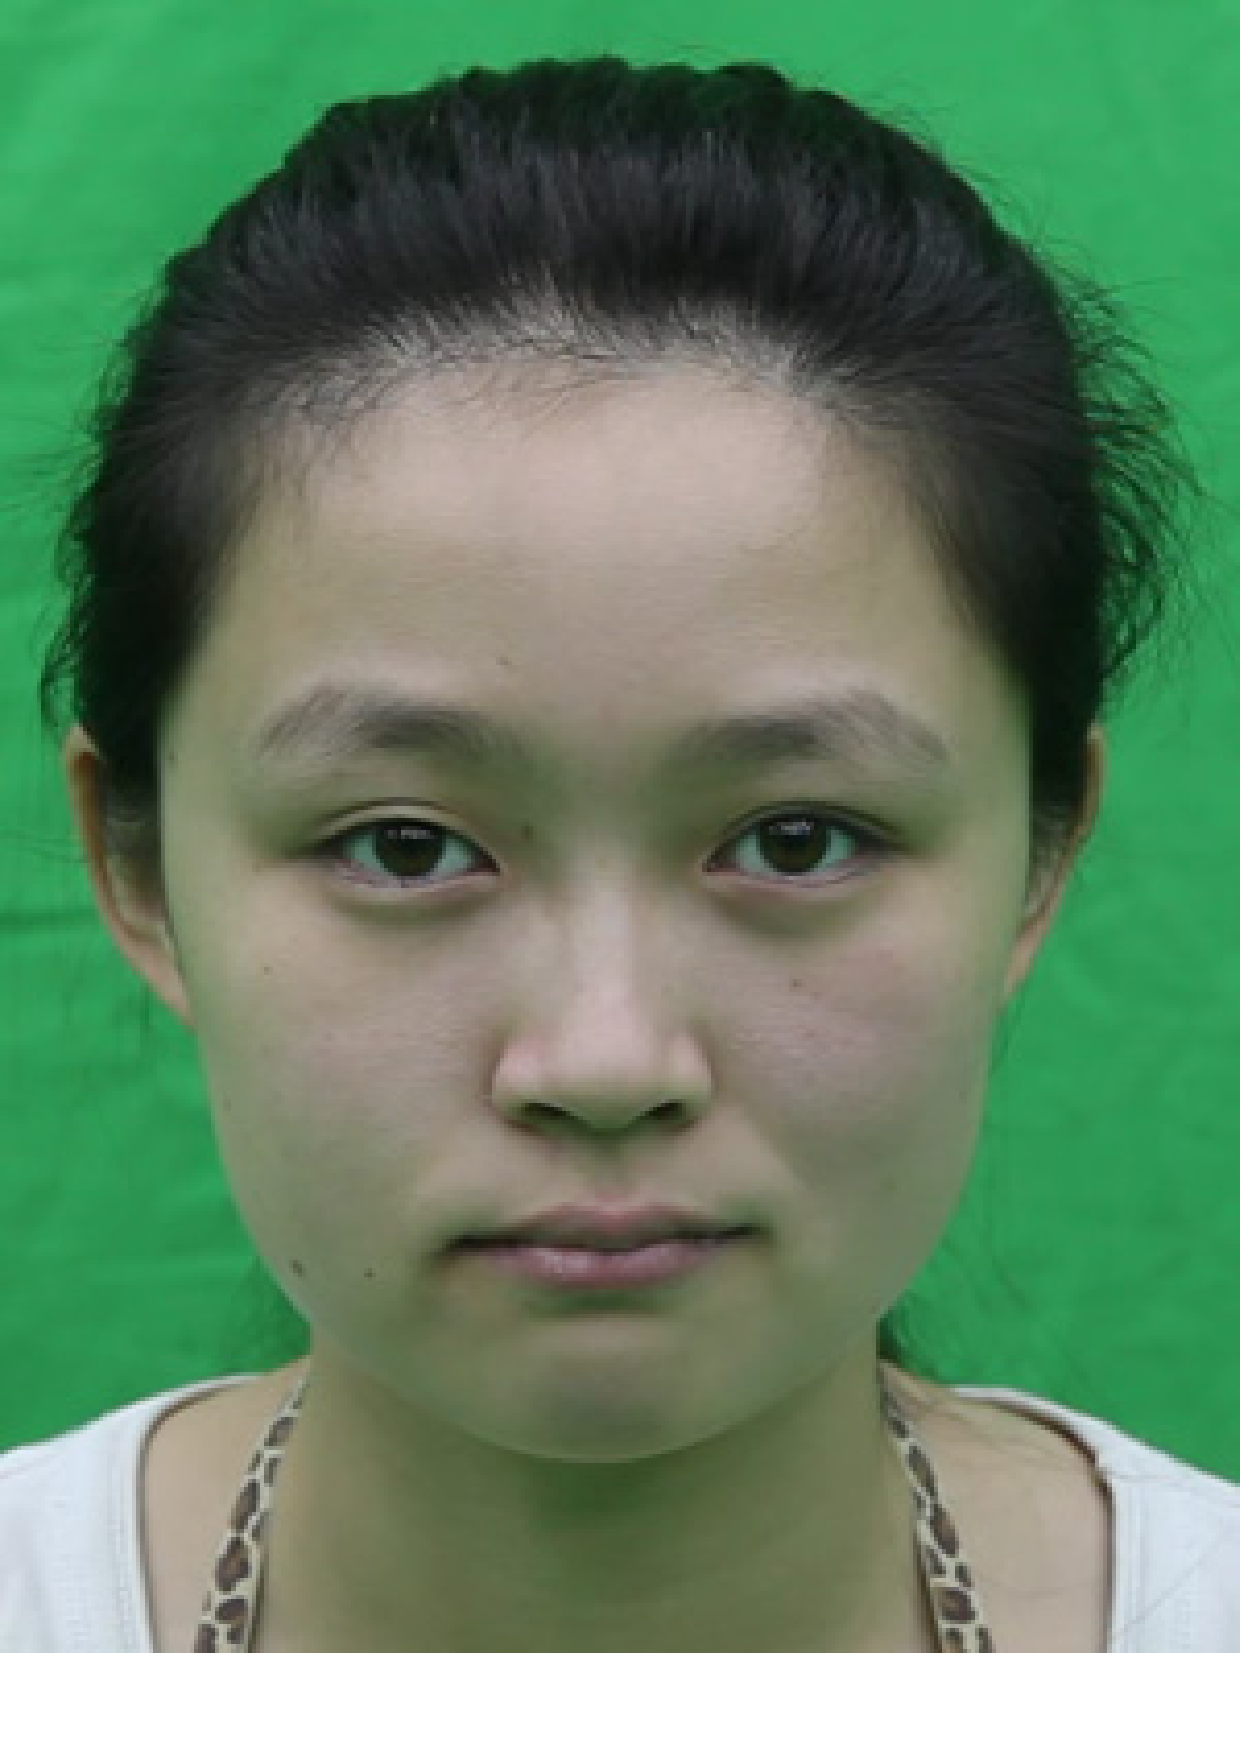
\includegraphics[width=0.23\textwidth]{data/img/velocity_without_00198.pdf}}
    \subcaptionbox{}{
    \label{fig:velocity_with}
    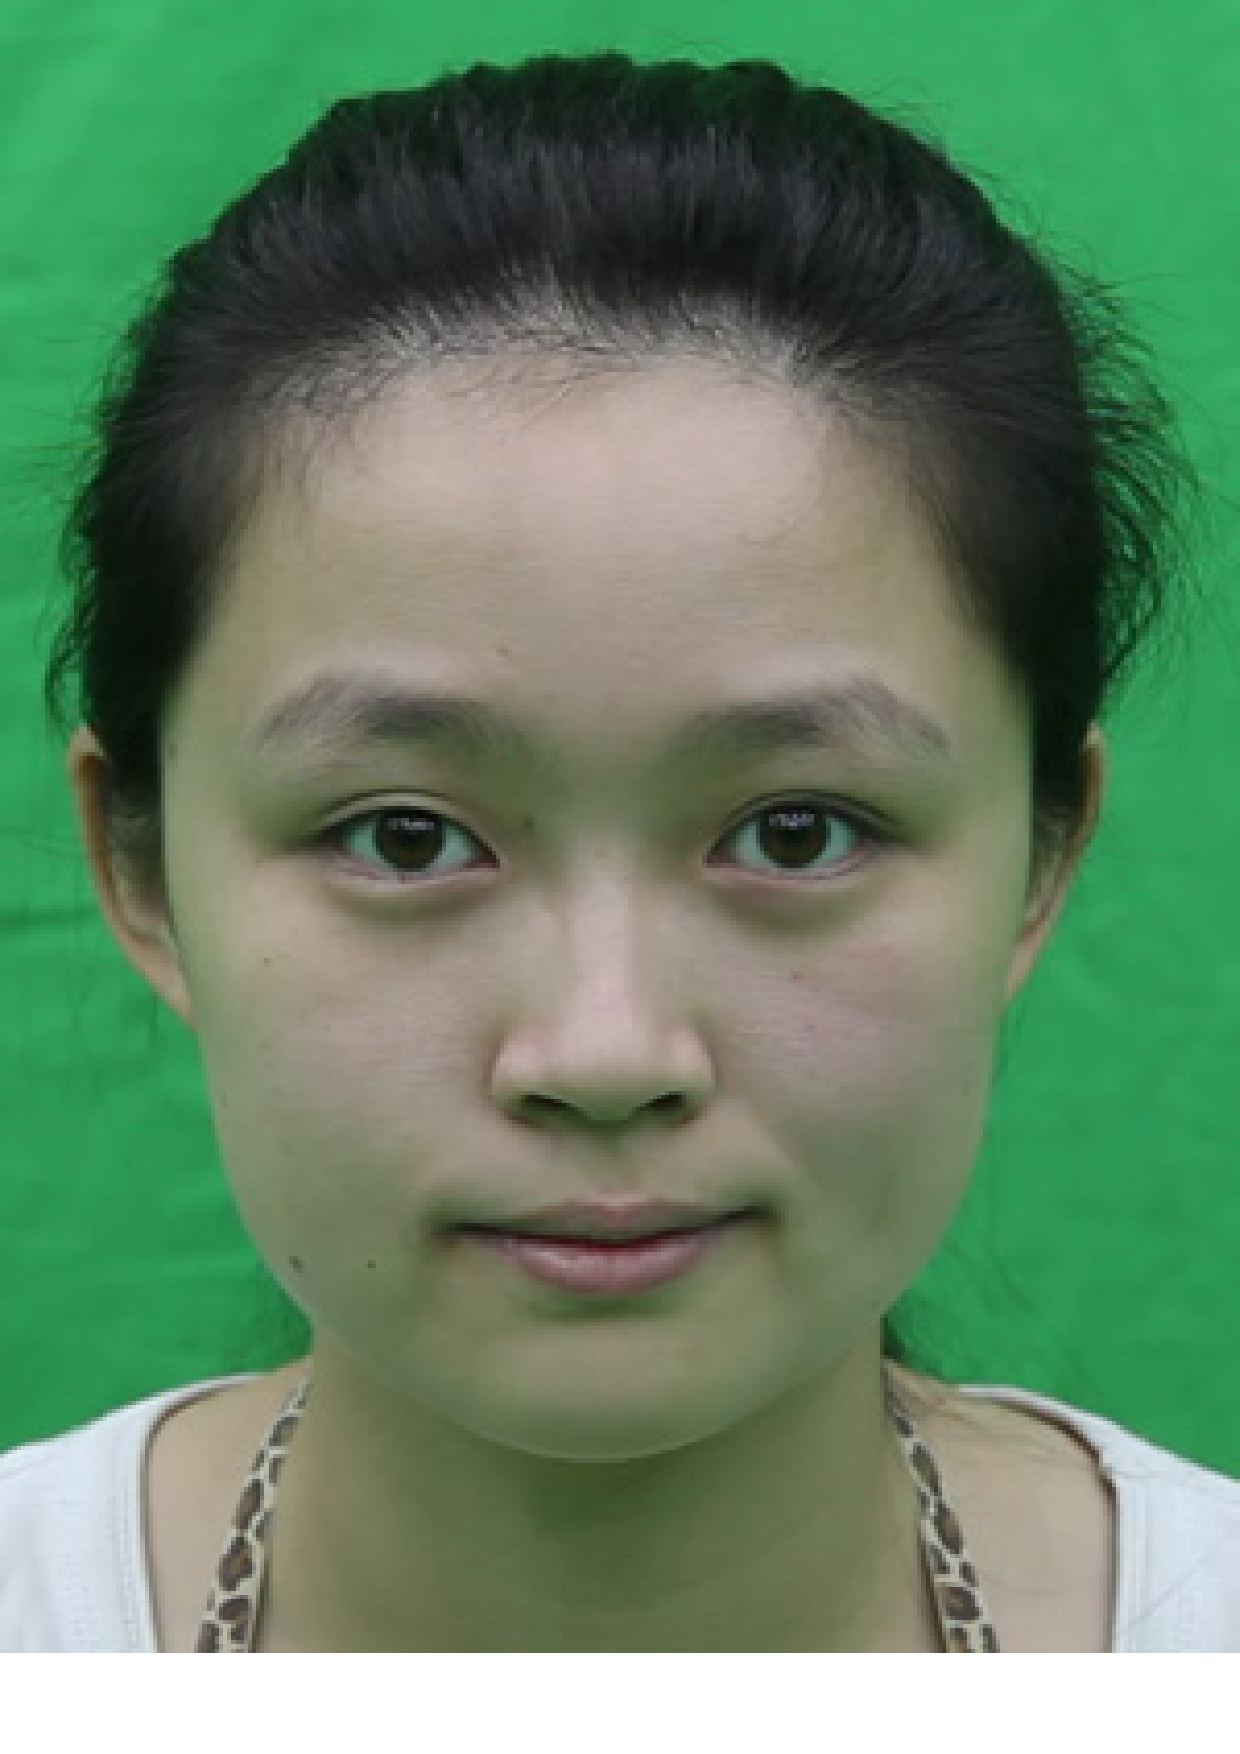
\includegraphics[width=0.23\textwidth]{data/img/velocity_with_00198.pdf}}
    \caption{使用表情速度的重要性阐述。(a) 红色表示带表情速度的当前查询帧。(b) 微笑的下一查询帧。(c) 由公式~\ref{eq:dist_comb}选择的最相似帧,有细淡淡的忧伤。(d)由公式~\ref{eq:dist_all}选择的最相似帧,有正确的微笑。}
    \label{fig:velocity}
\end{figure}

\subsubsection{基于优化的检索}
改进的表情相似度度量不能独立完整地解决时间一致性的问题。因此我们的系统使用就与优化的检索方法进一步提升合成序列的时间一致性。

对于每个查询帧,我们首先使用公式~\ref{eq:dist_all}定义的完整的距离度量从数据库不是抽取一个,而是$k$近邻,我们称之为候选帧。在每帧的时间戳放置一列$k$个候选帧,我们建立如图~\ref{fig:dijkstra}所示的有向无环图。有向边只连接邻近候选帧。记$V_i^{(q)}$ 为时刻$q$ 的第$i$候选帧。我们定义有向弧$r=(V_i^{(q)}, V_j^{(q+1)})$的长度为:
\begin{eqnarray}\label{eq:length}
\mathcal{L}(r)&=&\mathcal{D}(V_i^{(q)},Q_e^{(q)})+
        \mathcal{D}(V_j^{(q+1)},Q_e^{(q+1)})\nonumber\\
        &&+\lambda \exp ( - {{(\mathcal{T}(V_j^{(q + 1)} ) - \mathcal{T}(V_i^{(q)} ) - \mu )^2 }}/{{\sigma ^2 }}),
\end{eqnarray}

这里$\mathcal{T}(\cdot)$是输入帧的时间戳。通过最小化相邻帧的时间差,公式~\ref{eq:length} 的最后一项鼓励数据库中的连续帧选为匹配帧,以保证时间一致性。时间尺度变量$\mu$ 用于补偿查询和数据库序列之间的运动速度差。当查询帧和数据库序列运动速度大致相同,$\mu$设为1,当查询帧运动速度比数据库序列快则设为一个大数,否则相反。$\sigma$是带宽,$\lambda$是时间项的权重。

在公式~\ref{eq:length}中的时间项是L2范数,允许晓得时间变化,但对大的变化有严惩。由于小的变化被允许,它也允许某些时间尺度的变化。这在我们的查询序列1中被证明,如图~\ref{fig:result12}所示,它包含缓慢嘴巴张开的表情和快速撅嘴的表情。我们的系统对这二者都处理很好。此外,$\mu$也能在视频的不同时间根据查询运动的速度自动调整。

\begin{figure}[htbp]
\centering
    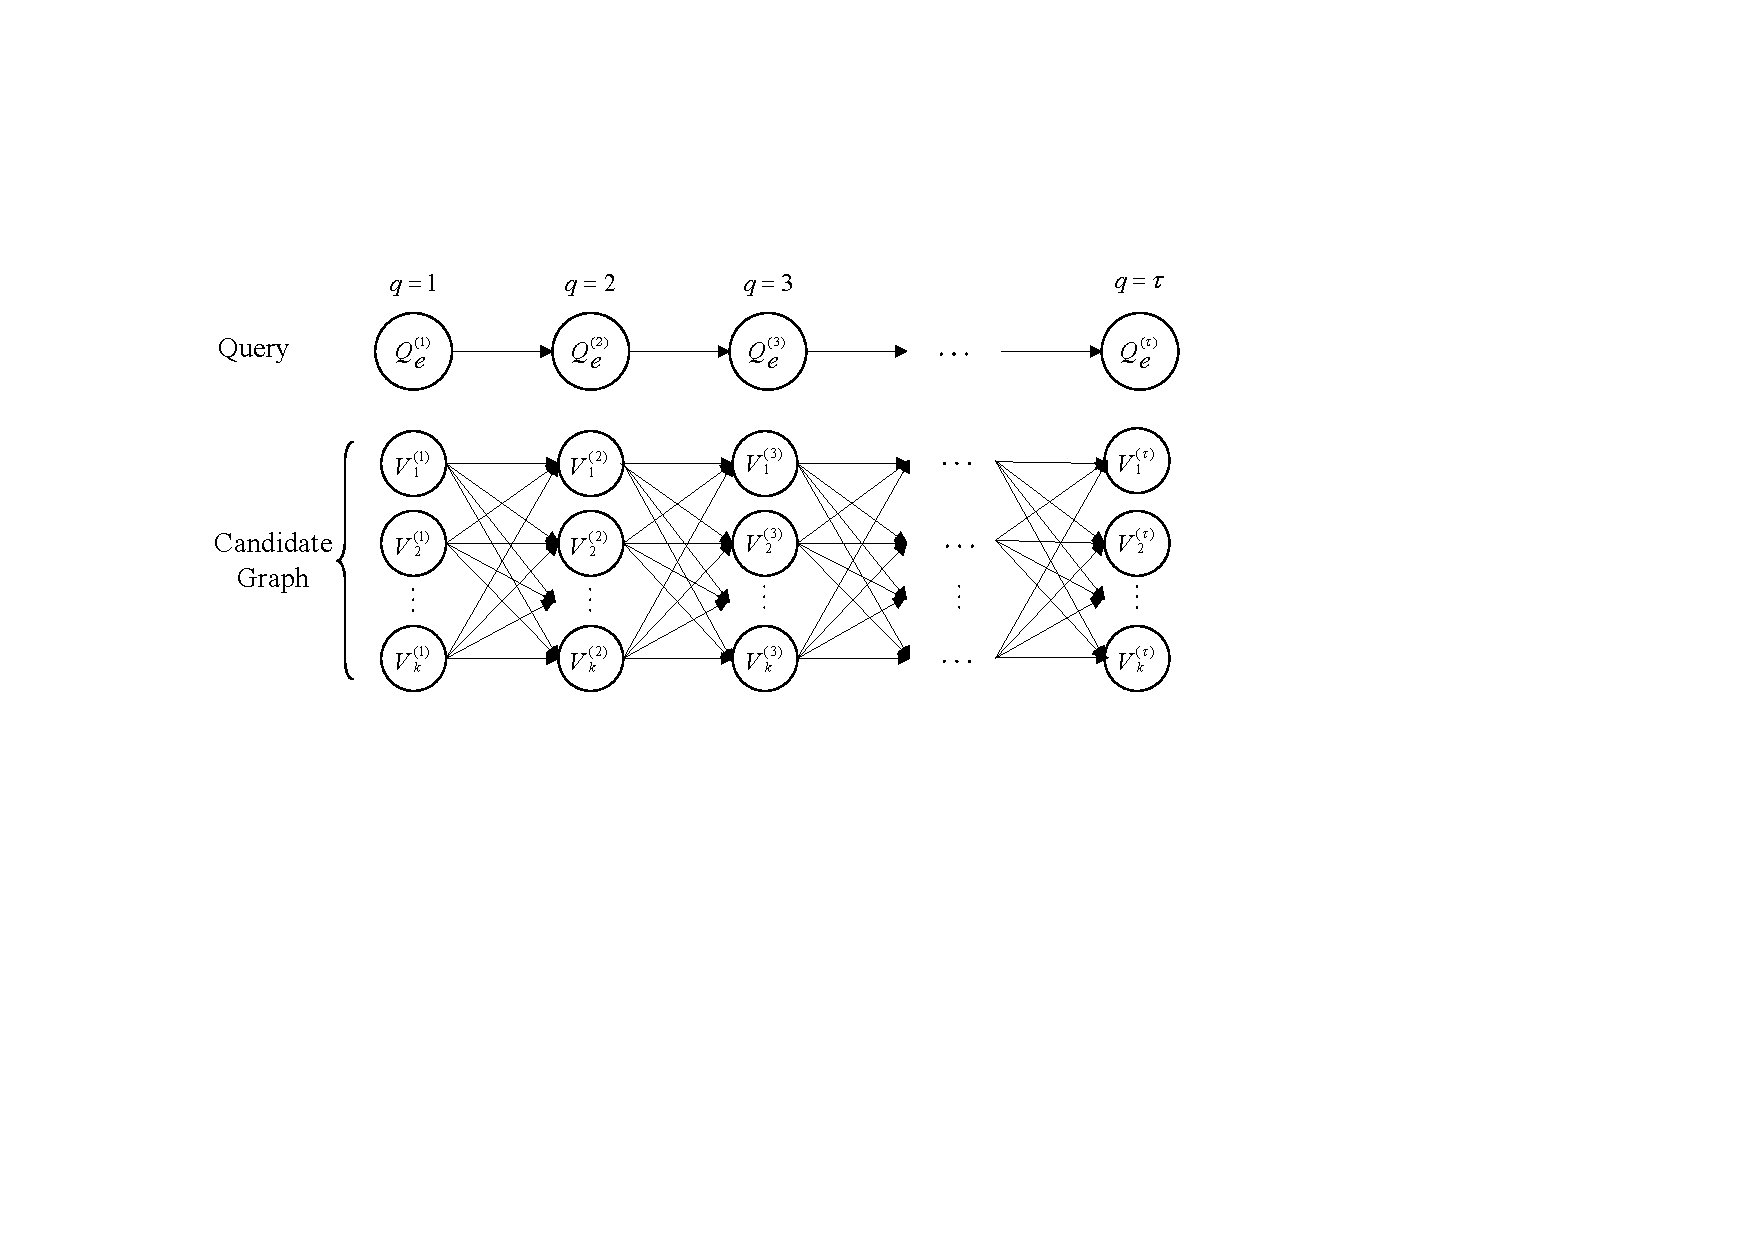
\includegraphics[width=0.90\textwidth]{data/img/dijkstra.pdf}
    \caption{用于检索的有向图}
    \label{fig:dijkstra}
\end{figure}

令$\mathcal{P}_{V_i^{(1)}\to V_j^{(\tau)}}$为连接起始节点$V_i^{(1)}$和终止节点$V_j^{(\tau)}$的路径,这里$i,j\in\{1,2,\ldots,k\}$。
在所有从第一到最后帧的可能路径中,我们找到最短路。优化目标被正式定义如下:
\begin{eqnarray}\label{eq:dijkstra}
\mathcal{P}_{opt}=\mathop{\arg\min}_{i, j} \mathop{\arg\min}_{\mathcal{P}_{V_i^{(1)}\to V_j^{(\tau)}}}
        \sum_{r\in \mathcal{P}_{V_i^{(1)}\to V_j^{(\tau)}}}\mathcal{L}(r).
\end{eqnarray}

该问题用Fibonacci堆~\cite{algorithm}的Dijkstra算法很好解决。连接最优路径$\mathcal{P}_{opt}$的所有帧构成检索序列。

我们的基于优化的方法借鉴了以往用于生成时间一致动画的工作~\cite{Kovar_Gleicher,spacetime,photobios}。我们的方法结合了时间一致性和语义对应。

\subsection{表情精炼}\label{sec:emi}
前面的检索结果有两个缺点。首先,由于我们的数据库的大小是有限的,检索的帧可能不包含和输入序列完全相同的表情。其次,数据库中的帧没完全对齐,所以检索序列包含了一些少量的时间抖动。要删除这些错误,我们的系统采用了额外的表情细化组成部分。

表情精炼的主要思路是给定$Q_n$ 和$Q_e$,中性帧和人偶师的表情帧,还有$T_n$,目标人的中性帧,我们可以直接从两个源图片中提取表情,并映射到$T_n$来合成新的面部$T_{Q_e}$。该合成的脸部,我们称之为expression mapping image(EMI),有所需的表情,但是也许没有逼真的纹理,尤其当$Q_n$ 和 $Q_e$表情差异很大的时候。另一方面,检索帧有真实的外表,但表情和$Q_e$并不完美匹配。结合EMI和检索帧,我们可以生成最终图片,有逼真的外表和精确匹配的表情。

具体说,我们首先通过把$Q_n$ 和$Q_e$的光流转移到目标帧来扭曲$T_n$。给定点$\vec{a}\in Q_n$,$\vec{a}'\in Q_e$和$\vec{b}\in T_n$ ($\vec{b}=g(\vec{a})$ 如公式~\ref{eq:map2}),我们计算点$\vec{b}'\in T_{Q_e}$ 的颜色如下:
\begin{equation}\label{eq:ratio}
c_{\vec{b}'}=c_{\vec{b}}\frac{c_{\vec{a}'}}{c_{\vec{a}}},
\end{equation}

这里$c_{\{\vec{a},\vec{a}',\vec{b},\vec{b}'\}}$分别是点$\vec{a}$, $\vec{a}'$, $\vec{b}$ and $\vec{b}'$的颜色值(我们系统中使用YCrCb颜色空间)。这里我们用比值${c_{\vec{a}'}}/{c_{\vec{a}}}$来表示颜色$c_{\vec{b}}$如ERI方法~\cite{eri}所做。在实际实施中,为了避免$\vec{b}'$有非整数坐标,我们用反向计算表情映射我们从一个整数像素$\vec{b}'\in T_{Q_e}$开始,根据$\vec{a}'=g^{-1}(b')$找到它的对应点$\vec{a}'\in Q_e$ 。通过计算\mbox{\boldmath $F$}$_{Q_e \to Q_n}$获得的光流$\Delta \vec{a}'$ 给出点$\vec{a}$的坐标。通过注册函数,我们获得点$\vec{b}=g(\vec{a})\in Q_n$的位置。然后点$\vec{b}'$ 的颜色可以依据公式\ref{eq:ratio} 计算。

\begin{figure}[htbp]
\centering
    \subcaptionbox{}{
    \label{fig:refine_driven}
    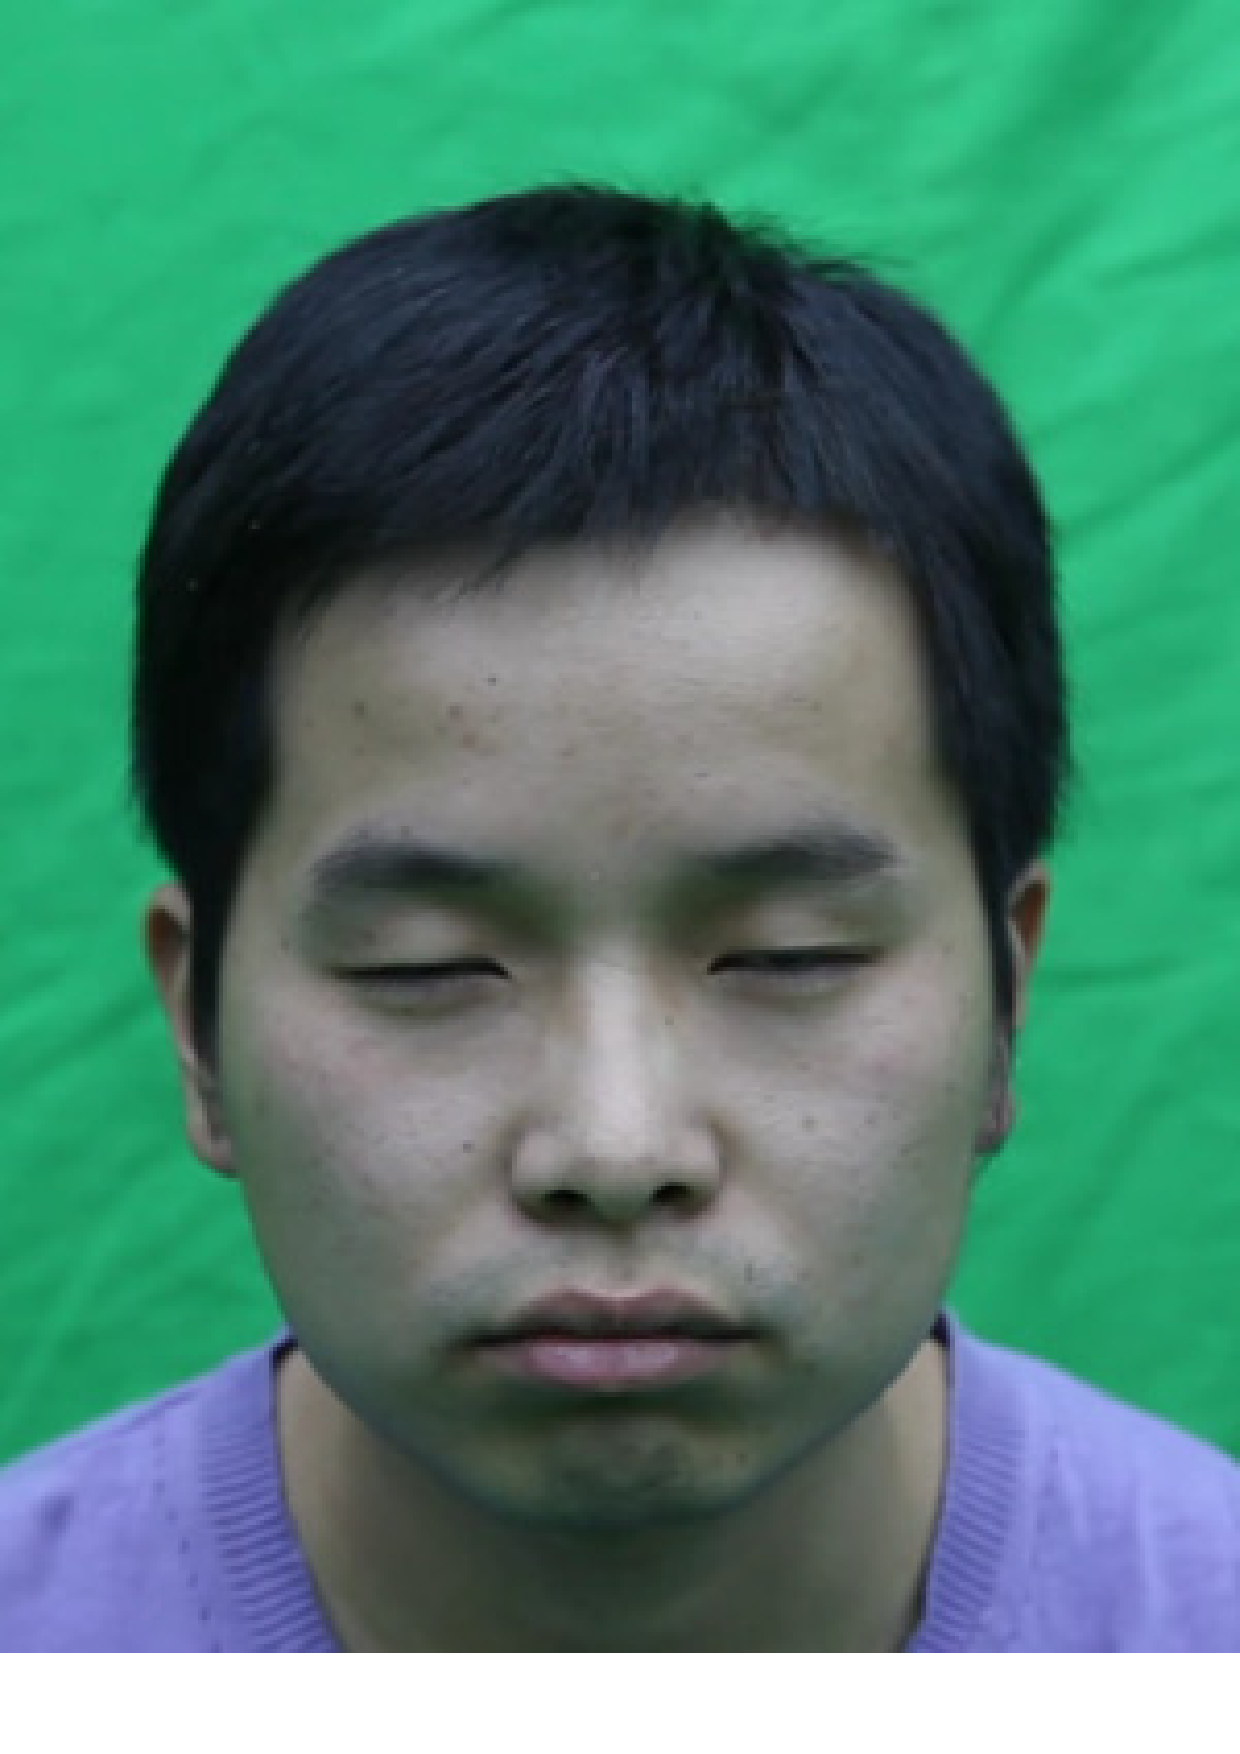
\includegraphics[width=0.23\textwidth]{data/img/refine_likai_0380_00151.pdf}}
    \subcaptionbox{}{
    \label{fig:refine_retrieval}
    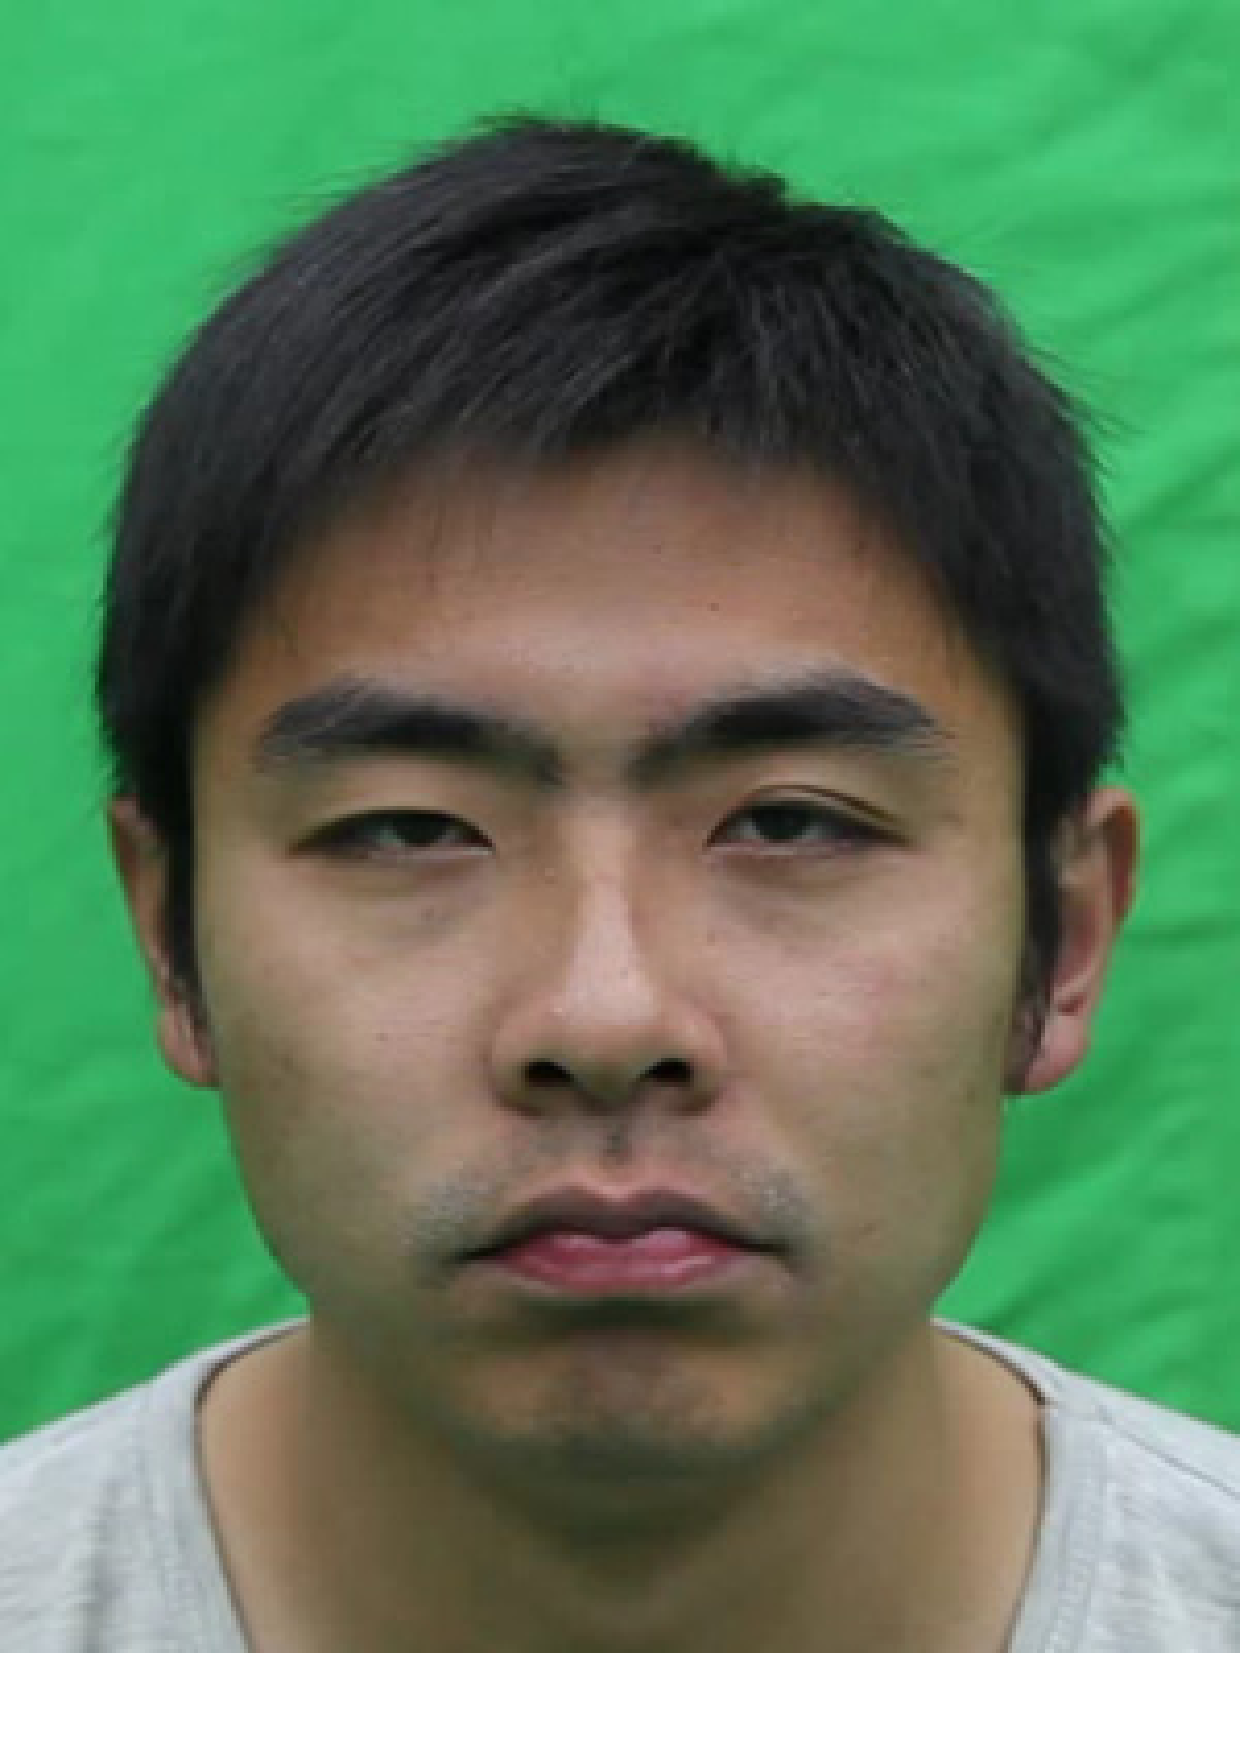
\includegraphics[width=0.23\textwidth]{data/img/refine_retrieval_00150.pdf}}
    \subcaptionbox{}{
    \label{fig:refine_emi}
    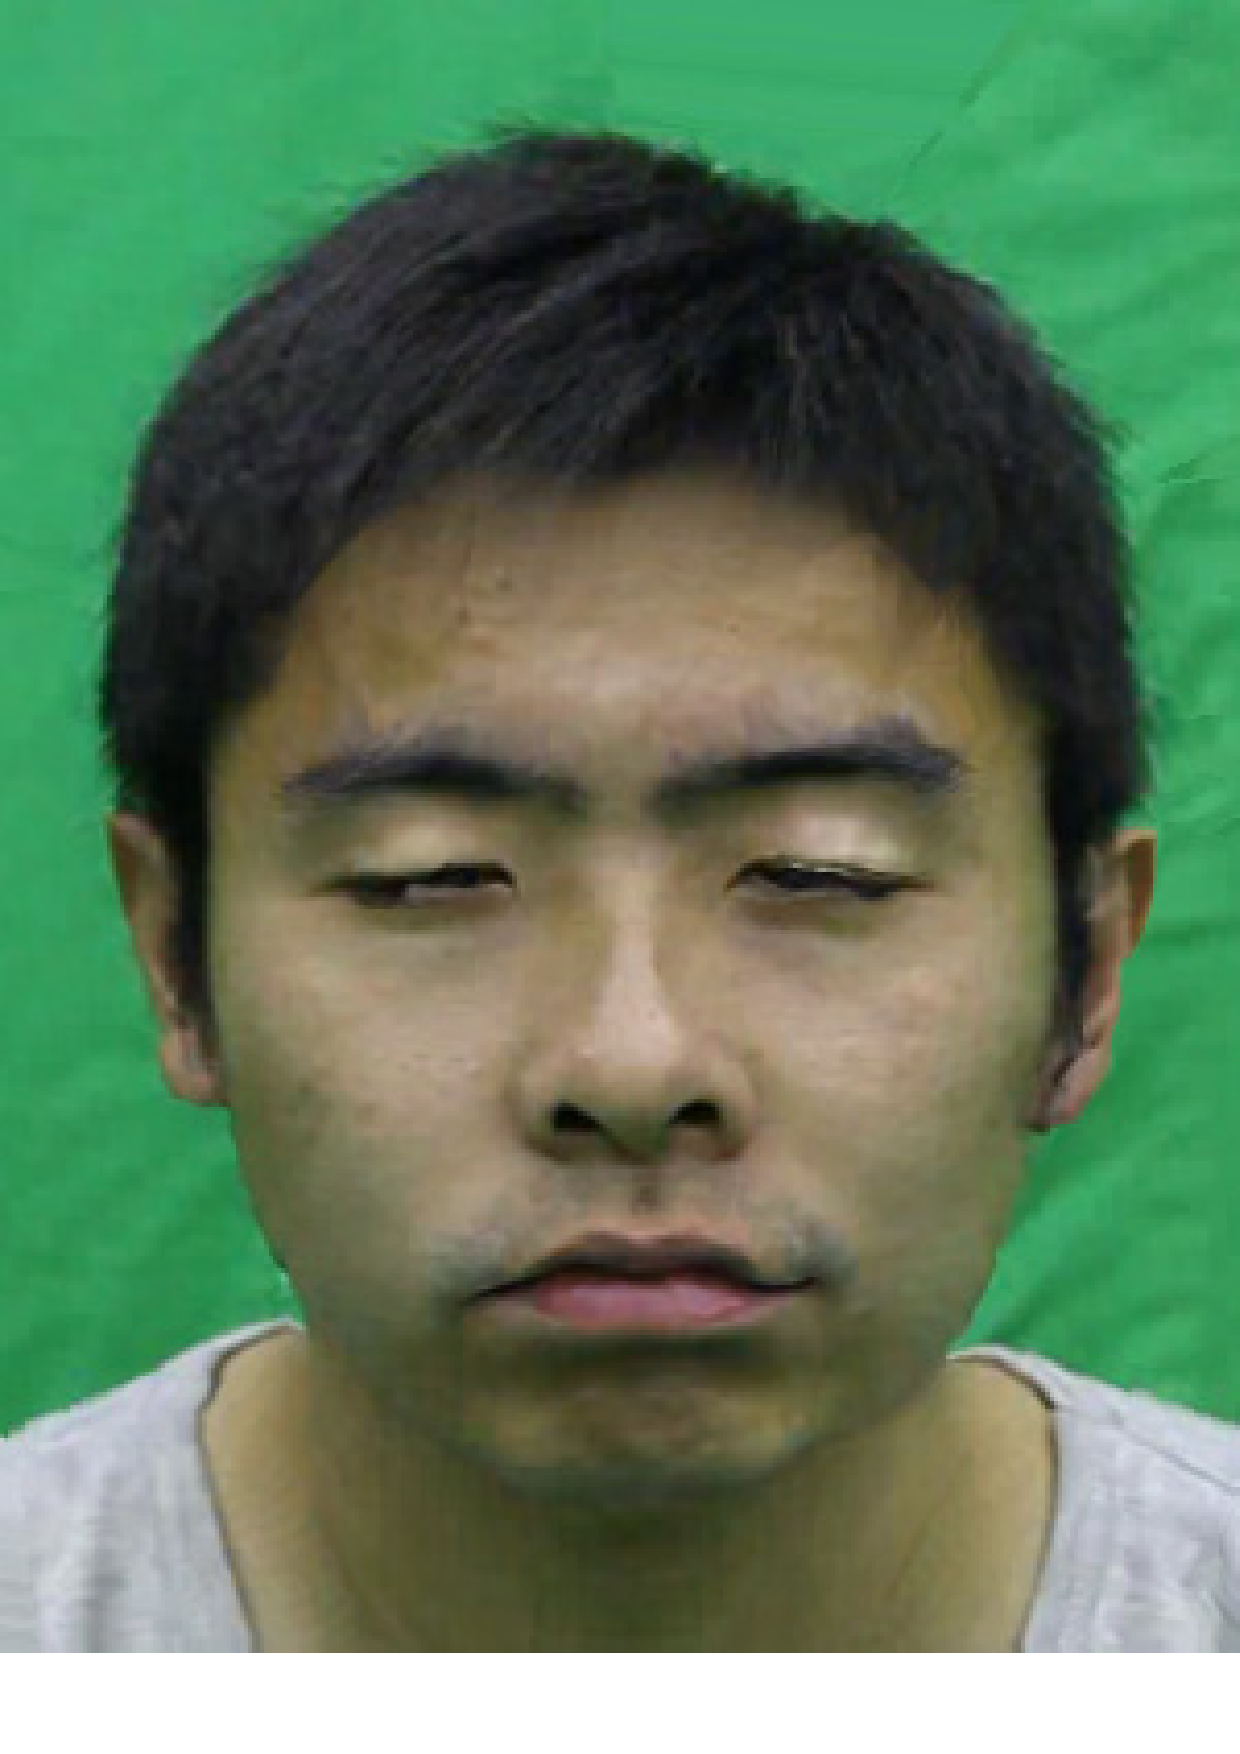
\includegraphics[width=0.23\textwidth]{data/img/refine_EMI_00151.pdf}}
    \subcaptionbox{}{
    \label{fig:refine_final}
    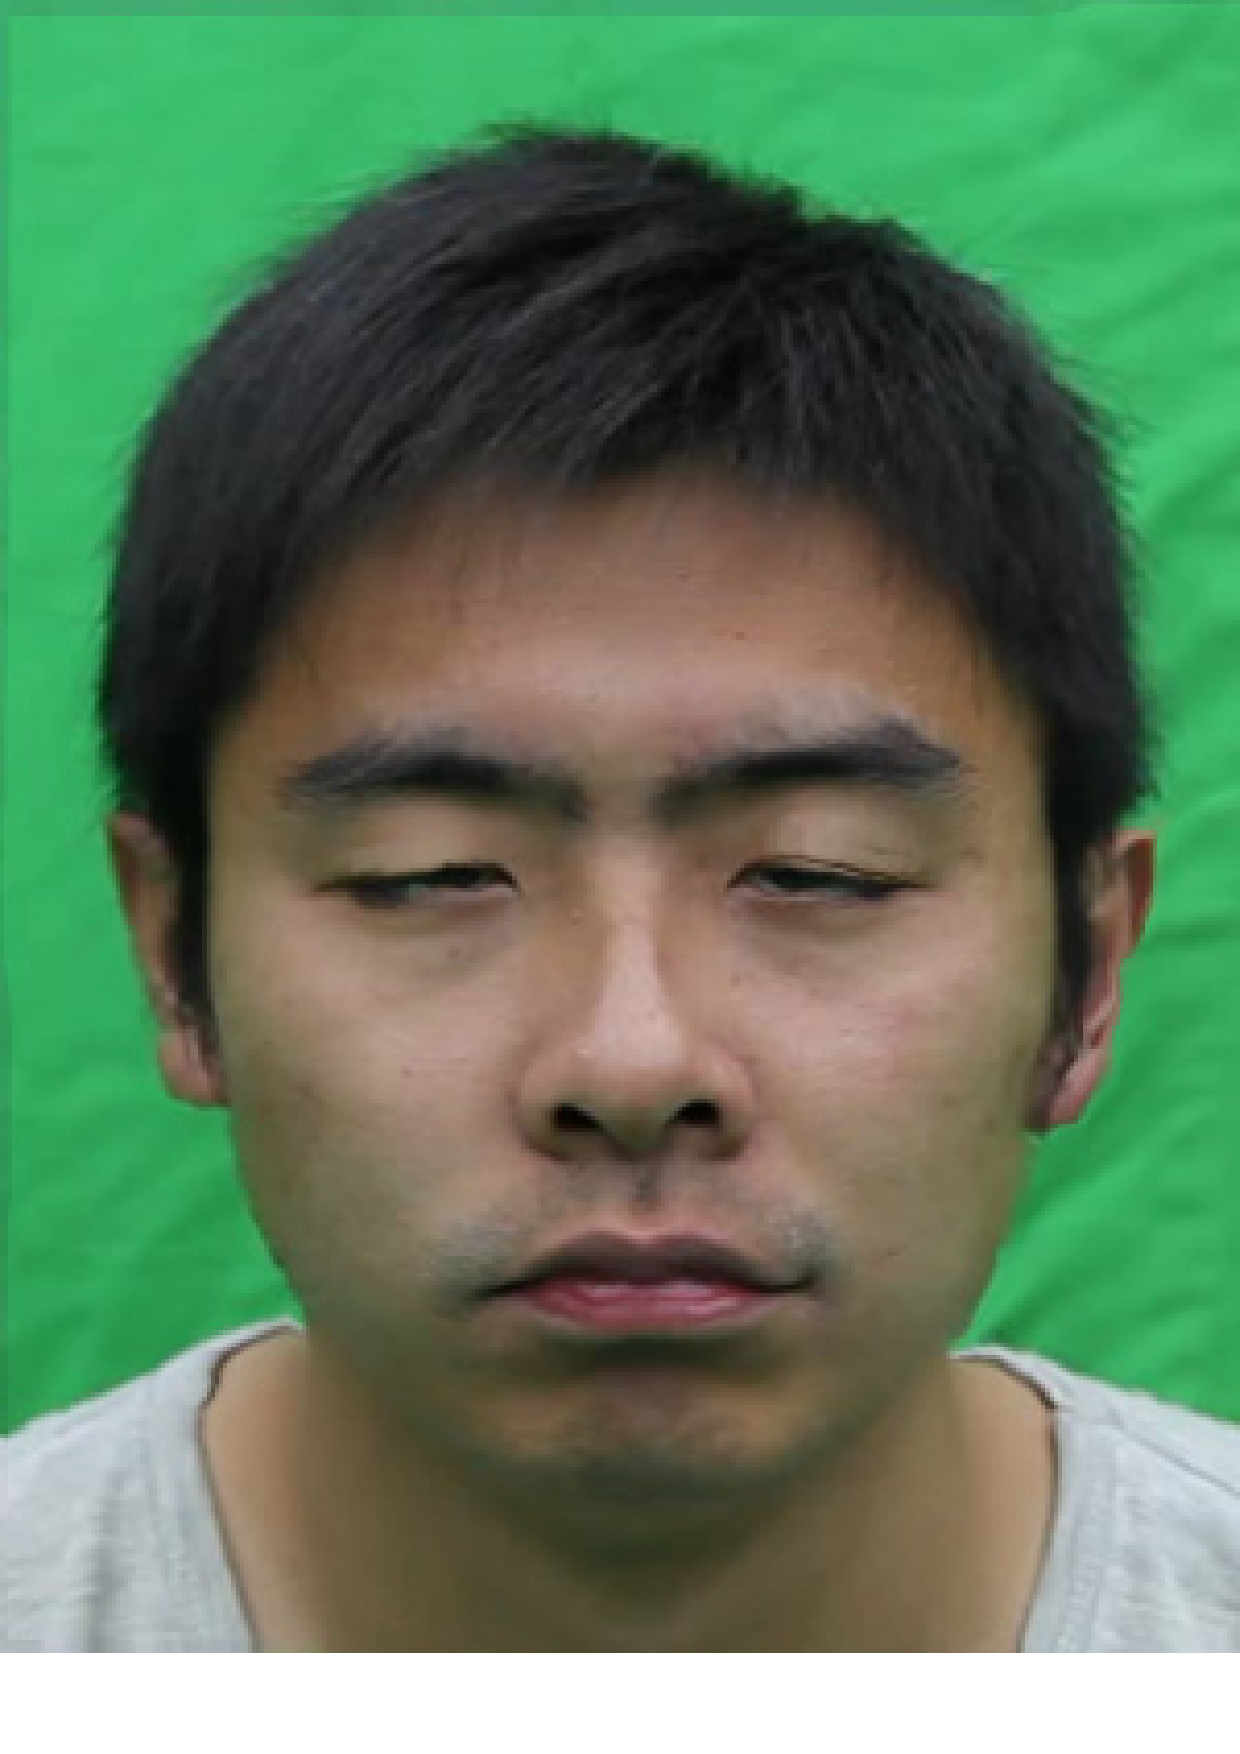
\includegraphics[width=0.23\textwidth]{data/img/refine_combine_00150.pdf}}
    \caption{表情精炼。 (a) 查询帧。 (b) 检索帧。 (c) 表情映射图片。 (d) 最终结果。}
    \label{fig:refine}
\end{figure}

最终,我们计算每一帧时的EMI和检索结果的光流,并利用光流扭曲检索图像至EMI。如图~\ref{fig:refine}所示,最终合成结果不只有从检索帧继承来的真实的外表,还有由EMI图像继承来的和查询帧匹配的正确表情。
\section{结论和讨论}
\begin{figure}[htbp]
\centering
    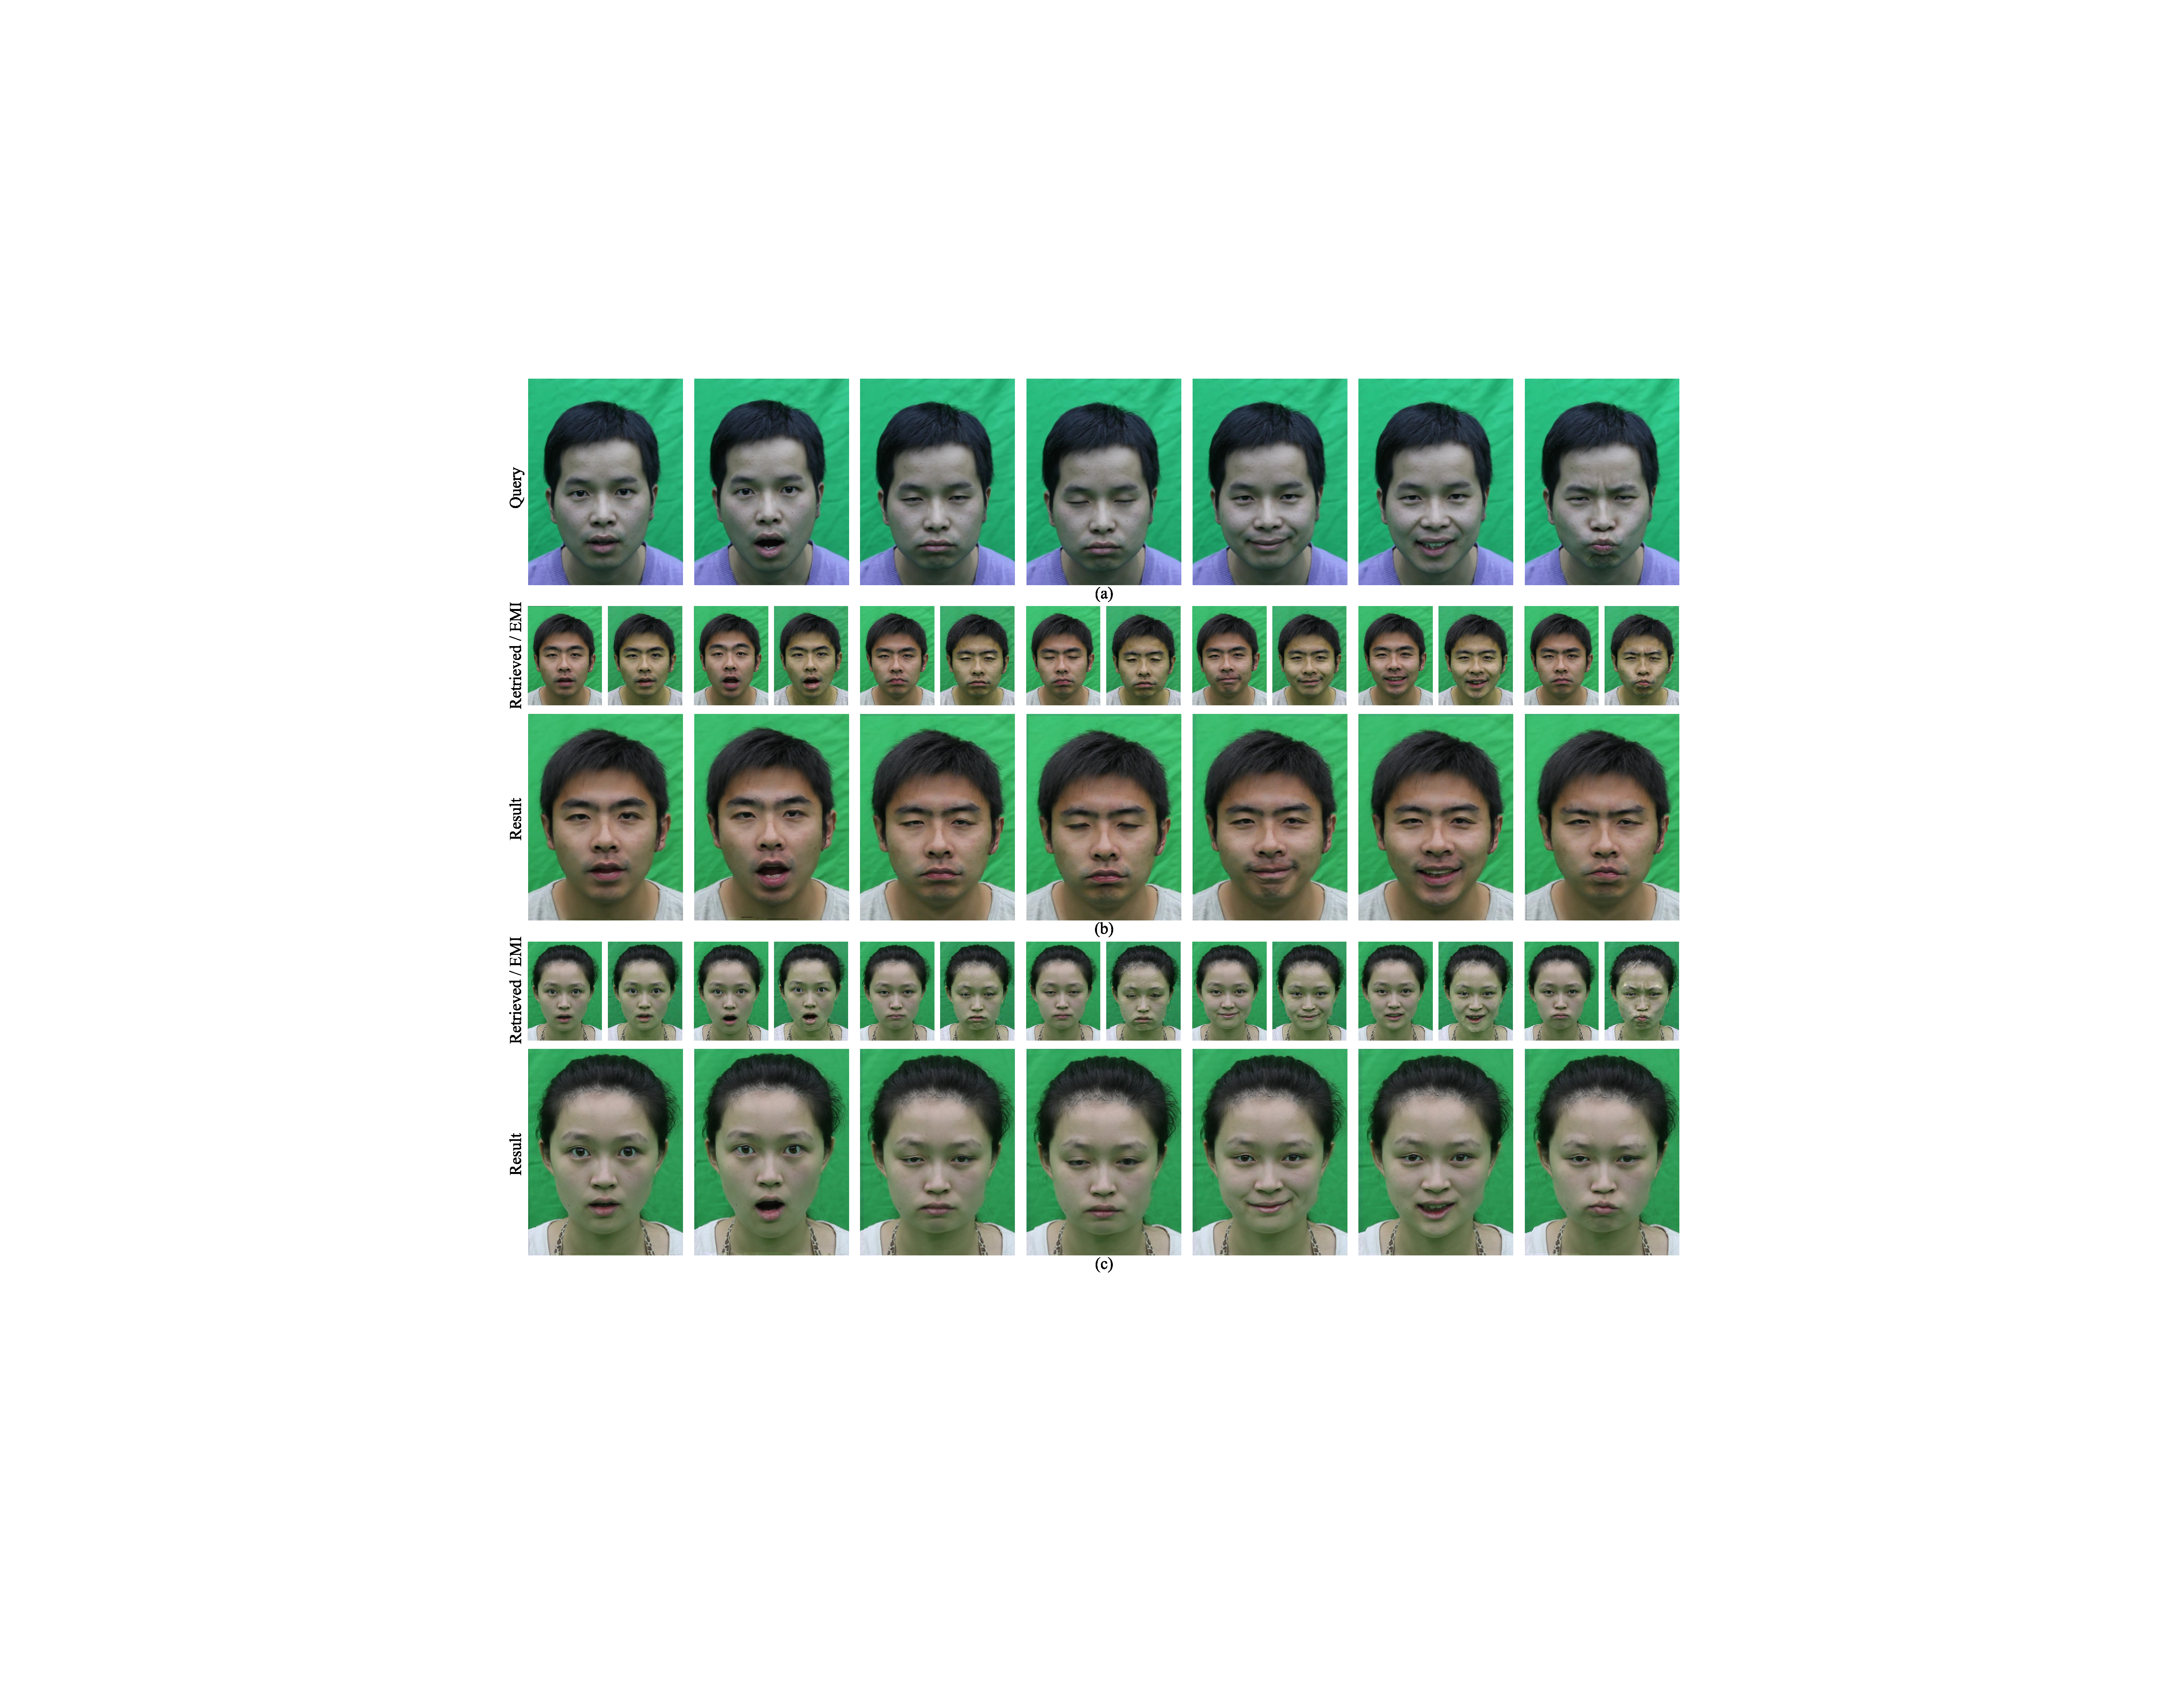
\includegraphics[width=0.9\textwidth]{data/img/likai2xf_jyy.pdf}
    \caption{在目标 $T1$ 和 $T2$ 上运行的查询序列的结果。 (a) 普通查询帧
    (b) (第一行)检索和EMI帧(分别是左和右);(第二行)目标 $T1$ 的最终合成帧。 (c) 目标 $T2$ 的检索、EMI帧和Retrieved最终合成帧。}
    \label{fig:result12}
\end{figure}

\subsection{实验}
我们评估了三个数据库系统。其中两个是我们采集的,这两个主题一个是男性,一个女性,他们被要求表现6个基本表情:愤怒,厌恶,惊讶,恐惧,快乐和悲伤。每个数据库都是25fps拍摄,包含约1500帧。第三个数据库是从Extended Cohn-Kanade Dataset (CK+) \cite{CK+}得到的 S130 。 S130 中的11个短序列(共220帧)构成了该表情数据库。在所有试验中,我们算法的参数固定如下:$\alpha_e=\frac{0.6}{n_{e}}$, $\alpha_m=\frac{0.4}{n_m}$, $\beta_m=0.9$, $\beta_o=0.1$,
$\gamma_e=0.9$, $\gamma_v=0.1$, $k=20$, $\lambda=0.1$, $\mu=1$, $\sigma=2$,其中 $n_e$ 和 $n_m$ 分别是目标中性面眼镜和嘴巴区域的像素数量。

\subsection{结果和评估}
图~\ref{fig:result12}显示了目标 $T1$(男性)和 $T2$ (女性)由输入序列驱动的合成结果。注意我们的系统不仅在诸如笑脸和惊奇等表情在数据库中时可以合成逼真的表情,而且在诸如撅嘴且双眼紧闭的表情在数据库中没有的时候也能合成新表情。同时,最终合成的视频也是时间相干的。图~\ref{fig:result3}展示了由另一序列驱动,从来自 CK+ 数据库的S130 中合成的结果。结果表明即使只是一个小数据库我们的系统仍然效果很好。可以在补充材料中找到包括额外的快速说话重定位结果的完整的视频序列。
为了评价我们的合成结果,我们进行了包含 $34$ 个参与者的用户研究。每位参与者都被展示了四个视频,分别由 LBP 特征查询方法~\cite{eccv10},在第~\ref{sec:emi}章介绍的 EMI 方法,我们的检索策略和我们的整套算法一帧一帧查询获得。每个视频并排展示了查询和结果。在实验中,参与者被要求根据表情的真实性和一致性评价在每个结果中表情的好坏,分数从 5(非常好)到 0(一点也不好)。表~\ref{tab:userstudy} 显示了3个目标的平均分。参与者发现我们的最终结果是最好的且我们的检索策略优于在~\cite{eccv10}提出的方法。
\renewcommand{\tablename}{表}
\begin{table}[htp]
\centering
    \begin{tabular}{|l|p{1cm}|p{1cm}|p{1cm}|}
    \hline
    & $T1$ & $T2$ & S130\\
    \hline\hline
    基于 LBP 的检索 \cite{eccv10} & 1.20 & $1.50$ & $1.38$\\
    我们的检索 & $2.49$ & $3.00$ & $2.56$\\
    EMI & $2.89$ & $1.91$ & $3.35$\\
    我们的整套系统 & $\mathbf{4.02}$ & $\mathbf{4.56}$ & $\mathbf{4.08}$\\
    \hline\hline
    $p$ 值 & $0.002$ & $0.005$ & $0.0001$ \\
    \hline
    \end{tabular}
    \caption{用户研究结果。该结果在统计上是有意义的,使用了单变量方差分析,$p$-value $<0.01$。}
    \label{tab:userstudy}
\end{table}

\subsection{局限性}
我们目前的系统只针对正面脸部表情合成设计。可能会扩展系统在大旋转角下运行,通过稀疏相机阵列采集数据。如此我们需要估计表情和输入帧的3D脸部。此外,需要视图变形技术~\cite{ViewMorphing}来在不同视角查看脸部,以在所需姿态生成面部表情。

另一个限制是,当表情很极端,传统的光溜方法无法精确捕捉表情差异。除了调查更好的脸部光流技术,另一个解决方案是为每个特征使用多个预先对其的脸部图像而不只是在我们现有系统中使用单一中性面。

\begin{figure*}[htbp]
\centering
    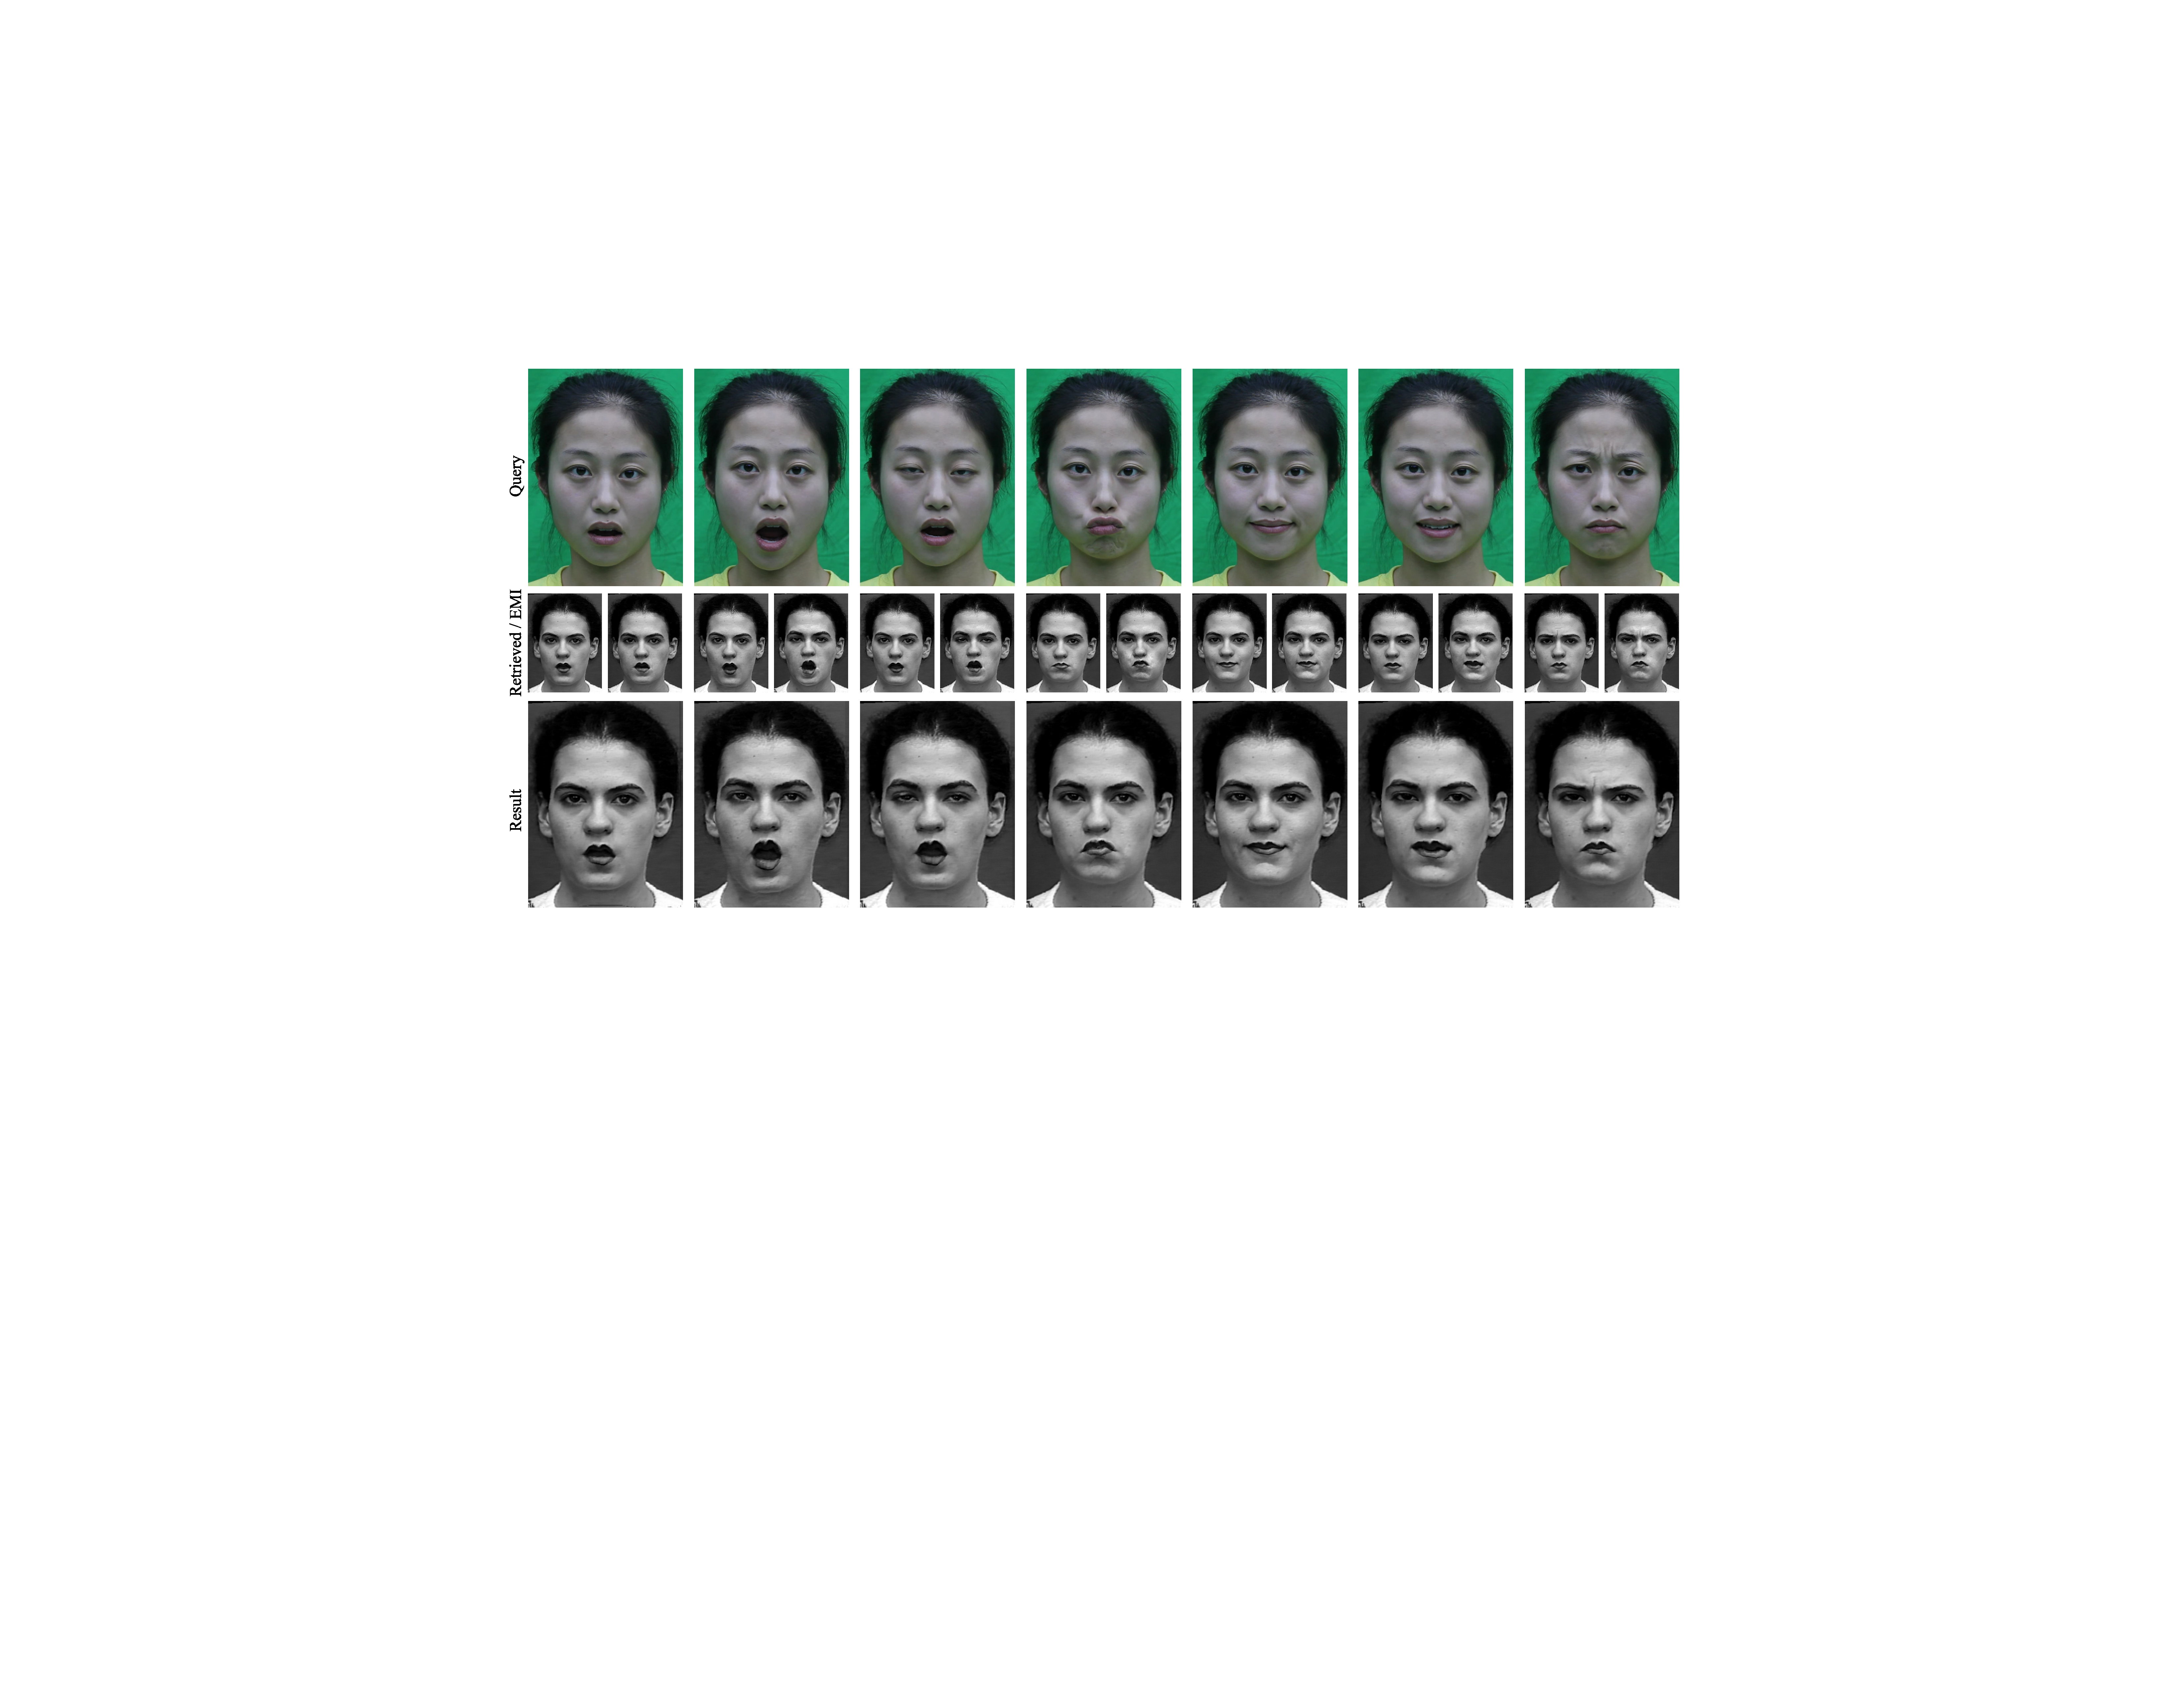
\includegraphics[width=0.90\textwidth]{data/img/liwen2S130.pdf}
    \caption{在来自CK+的S130中由查询序列2获得的结果。 (顶部)查询帧。(中部)检索帧和EMI 帧(分别是左和右)。(底部)最终合成帧。}
    \label{fig:result3}
\end{figure*}

\section{结论}

我们提出了一种数据驱动的方法来用一个人的面部表情视频对目标人脸合成真实的面部动画。我们的系统采用了新颖的时空表情距离度量,可以准确地测量视频中不同的人相似的表情。我们也提出了最短路径优化的检索策略来平衡在最终视频的表情相似性和时间连续性。和那些直接表情映射相比,通过变换检索到的视频帧进一步改善了表情相似性。用户研究结果表明,我们的系统可以产生很高的保真度和时间上一致的面部动画。

\section*{致谢}
作者要感谢和王瑞平,邓岳,索津莉的讨论,评审和领导建设性的意见。这项研究由国家自然科学基金项目支持(第61035002号,第61073072号,第60933006号)。

\setcounter{NAT@ctr}{0}%
\renewcommand{\refname} {参考文献}
{\small
\bibliographystyle{ieee}
\pagestyle{empty}
\bibliography{egbib}
}

%  \input{data/appendix02}
% \end{appendix}
% \end{example}
%
% \myentry{致谢声明}
% \DescribeEnv{ack}
% 把致谢做成一个环境更好一些,直接往里面写感谢的话就可以啦!下面是数学系一位同
% 学致谢里的话,拿过来做个广告,多希望每个人都能写这么一句啊!
% \begin{example}
% \begin{ack}
%   ……
%   还要特别感谢计算机系薛瑞尼同学在论文格式和 \LaTeX{} 编译等方面给我的很多帮助!
% \end{ack}
% \end{example}
%
% \myentry{列表环境}
% \DescribeEnv{itemize}
% \DescribeEnv{enumerate}
% \DescribeEnv{description}
% 为了适合中文习惯,模板将这三个常用的列表环境用 \pkg{paralist} 对应的压缩环境替
% 换。一方面满足了多余空间的清楚,另一方面可以自己指定标签的样式和符号。细节请参
% 看 \pkg{paralist} 文档,此处不再赘述。
%
% \changes{v3.0}{2007/05/12}{没有了综合论文训练页面,很多本科论文专用命令就消失了。}
%
% \subsection{数学环境}
% \label{sec:math}
% \thuthesis{} 定义了常用的数学环境:
%
% \begin{center}
% \begin{tabular}{*{7}{l}}\hline
%   axiom & theorem & definition & proposition & lemma & conjecture &\\
%   公理 & 定理 & 定义 & 命题 & 引理 & 猜想 &\\\hline
%   proof & corollary & example & exercise & assumption & remark & problem \\
%   证明 & 推论 & 例子& 练习 & 假设 & 注释 & 问题\\\hline
% \end{tabular}
% \end{center}
%
% 比如:
% \begin{example}
% \begin{definition}
% 道千乘之国,敬事而信,节用而爱人,使民以时。
% \end{definition}
% \end{example}
% 产生(自动编号):\\[5pt]
% \fbox{{\heiti 定义~1.1~~~} {道千乘之国,敬事而信,节用而爱人,使民以时。}}
%
% 列举出来的数学环境毕竟是有限的,如果想用{\heiti 胡说}这样的数学环境,那么很容易定义:
% \begin{example}
% \newtheorem{nonsense}{胡说}[chapter]
% \end{example}
%
% 然后这样使用:
% \begin{example}
% \begin{nonsense}
% 契丹武士要来中原夺武林秘笈。\pozhehao 慕容博
% \end{nonsense}
% \end{example}
% 产生(自动编号):\\[5pt]
% \fbox{{\heiti 胡说~1.1~~~} {契丹武士要来中原夺武林秘笈。\kern0.3ex\rule[0.8ex]{2em}{0.1ex}\kern0.3ex 慕容博}}
%
% \subsection{自定义以及其它}
% \label{sec:othercmd}
% 模板的配置文件 thuthesis.cfg 中定义了很多固定词汇,一般无须修改。如果有特殊需求,
% 推荐在导言区使用 \cs{renewcommand}。当然,导言区里可以直接使用中文。
%
%
% \section{致谢}
% \label{sec:thanks}
% 感谢这些年来一直陪伴 \thuthesis{} 成长的新老同学,大家的需求是模板前
% 进的动力,大家的反馈是模板提高的机会。
% 
% 此版本加入了博士后出站报告的支持,本意为制作一个支持清华所有学位报告
% 的模板,孰料学校于近期对硕士、博士论文规范又有调整,未能及时更新,见
% 谅!
%
% 本人已于近期离开清华,虽不忍模板存此瑕疵,然精力有限,必不能如往日及
% 时升级,还望新的同学能参与或者接手,继续为大家服务。
% 
% \StopEventually{\PrintChanges\PrintIndex}
% \clearpage
%
% \section{实现细节}
%
% \subsection{基本信息}
%    \begin{macrocode}
%<cls>\NeedsTeXFormat{LaTeX2e}[1999/12/01]
%<cls>\ProvidesClass{thuthesis}
%<cfg>\ProvidesFile{thuthesis.cfg}
%<cls|cfg>[2012/07/28 4.8dev Tsinghua University Thesis Template]
%    \end{macrocode}
%
% \subsection{定义选项}
% \label{sec:defoption}
% TODO: 所有的选项用 \pkg{xkeyval} 来重构,现在的太罗唆了。
%
% 定义论文类型以及是否涉密
% \changes{v2.4}{2006/04/14}{添加模板名称命令。}
% \changes{v2.5}{2006/05/19}{增加本科论文的提交选项 submit。}
% \changes{v2.5.1}{2006/05/24}{如果没有设置格式选项,报错。}
% \changes{v2.5.1}{2006/05/26}{submit 只能由本科用。}
% \changes{v2.5.3}{2006/06/03}{submit 选项的一个笔误。}
% \changes{v3.0}{2007/05/12}{删除 submit 选项。}
% \changes{v4.6}{2011/04/26}{增加 postdoctor 选项。}
%    \begin{macrocode}
%<*cls>
\hyphenation{Thu-Thesis}
\def\thuthesis{\textsc{ThuThesis}}
\def\version{4.8}
\newif\ifthu@bachelor\thu@bachelorfalse
\newif\ifthu@master\thu@masterfalse
\newif\ifthu@doctor\thu@doctorfalse
\newif\ifthu@postdoctor\thu@postdoctorfalse
\newif\ifthu@secret\thu@secretfalse
\DeclareOption{bachelor}{\thu@bachelortrue}
\DeclareOption{master}{\thu@mastertrue}
\DeclareOption{doctor}{\thu@doctortrue}
\DeclareOption{postdoctor}{\thu@postdoctortrue}
\DeclareOption{secret}{\thu@secrettrue}
%    \end{macrocode}
%
% \changes{v2.5.1}{2006/05/24}{如果选项设置了 dvips,但是用 pdflatex 编译,报错。}
% \changes{v2.6}{2006/06/09}{增加 dvipdfm 选项。}
% \changes{v4.5}{2009/01/03}{增加 xetex, pdftex 选项。}
% \changes{v4.8dev}{2013/03/02}{内部调用 ctex 宏包,自动检测编译引擎}
%
% 如果需要使用 arial 字体,请打开 [arial] 选项
%    \begin{macrocode}
\newif\ifthu@arial
\DeclareOption{arial}{\thu@arialtrue}
%    \end{macrocode}
%
% 目录中英文是否用 arial
%    \begin{macrocode}
\newif\ifthu@arialtoc
\DeclareOption{arialtoc}{\thu@arialtoctrue}
%    \end{macrocode}
% 章节标题中的英文是否用 arial
%    \begin{macrocode}
\newif\ifthu@arialtitle
\DeclareOption{arialtitle}{\thu@arialtitletrue}
%    \end{macrocode}
%
% noraggedbottom 选项
% \changes{4.8dev}{2013/03/05}{增加 noraggedbottom 选项。}
%    \begin{macrocode}
\newif\ifthu@raggedbottom\thu@raggedbottomtrue
\DeclareOption{noraggedbottom}{\thu@raggedbottomfalse}
%    \end{macrocode}
%
% 将选项传递给 ctexbook 类
%    \begin{macrocode}
\DeclareOption*{\PassOptionsToClass{\CurrentOption}{ctexbook}}
%    \end{macrocode}
%
% \cs{ExecuteOptions} 的参数之间用逗号分割,不能有空格。开始不知道,折腾了老半
% 天。
% \changes{v2.5.1}{2006/05/24}{ft,研究生院目录要 times,而教务处要 arial。}
% \changes{v2.5.1}{2006/05/26}{本科 openright,研究生 openany。}
% \changes{v3.1}{2007/10/09}{本科的目录又不要 arial 字体了。}
% \changes{v4.8dev}{2013/03/10}{使用 ctexbook 类,优于调用 ctex 宏包。}
%    \begin{macrocode}
\ExecuteOptions{utf,arialtitle}
\ProcessOptions\relax
\LoadClass[cs4size,a4paper,openany,UTF8]{ctexbook}
%    \end{macrocode}
%
% 用户至少要提供一个选项:指定论文类型。
%    \begin{macrocode}
\ifthu@bachelor\relax\else
  \ifthu@master\relax\else
    \ifthu@doctor\relax\else
      \ifthu@postdoctor\relax\else
        \ClassError{thuthesis}%
                   {You have to specify one of thesis options: bachelor, master or doctor.}{}
      \fi
    \fi
  \fi
\fi
%    \end{macrocode}
%
% \subsection{装载宏包}
% \label{sec:loadpackage}
%
% 引用的宏包和相应的定义。
%    \begin{macrocode}
\RequirePackage{ifxetex}
\RequirePackage{ifthen,calc}
%    \end{macrocode}
%
% \AmSTeX{} 宏包,用来排出更加漂亮的公式。
% \changes{v4.8}{2013/03/02}{no need to load amssymb since we use txfonts.}
%    \begin{macrocode}
\RequirePackage{amsmath}
%    \end{macrocode}
%
% 用很爽的 \pkg{txfonts} 替换 \pkg{mathptmx} 宏包,同时用它自带的 typewriter 字
% 体替换 courier。必须出现在 \AmSTeX{} 之后。
% \changes{v3.1}{2007/06/16}{replace mathptmx with txfonts.}
%    \begin{macrocode}
\RequirePackage{txfonts}
%    \end{macrocode}
%
% 图形支持宏包。
%    \begin{macrocode}
\RequirePackage{graphicx}
%    \end{macrocode}
%
% 并排图形。\pkg{subfigure}、\pkg{subfig} 已经不再推荐,用新的 \pkg{subcaption}。
% 浮动图形和表格标题样式。\pkg{caption2} 已经不推荐使用,采用新的 \pkg{caption}。
%    \begin{macrocode}
\RequirePackage[labelformat=simple]{subcaption}
%    \end{macrocode}
%
% \changes{v4.8}{2013/03/02}{no need to load indentfirst directly since we use ctex.}
%
% 更好的列表环境。
% \changes{v2.6.2}{2006/06/18}{去掉 \pkg{paralist} 的 newitem 和 newenum 选项,因为默
% 认是打开的。}
% \changes{v2.6.4}{2006/10/23}{增加 \texttt{neverdecrease} 选项。}
%    \begin{macrocode}
\RequirePackage[neverdecrease]{paralist}
%    \end{macrocode}
%
% raggedbottom,禁止Latex自动调整多余的页面底部空白,并保持脚注仍然在底部。
%    \begin{macrocode}
\ifthu@raggedbottom
  \RequirePackage[bottom]{footmisc}
  \raggedbottom
\fi
%    \end{macrocode}
%
% 中文支持,我们使用 ctex 宏包。
% \changes{v4.5}{2008/01/03}{加入 XeTeX 支持,需要 \pkg{xeCJK}。}
% \changes{v4.8dev}{2013/03/09}{reset baselinestretch after ctex's change.}
%    \begin{macrocode}
\renewcommand{\baselinestretch}{1.0}
\ifxetex
  \xeCJKsetup{AutoFakeBold=true,AutoFakeSlant=true}
  \punctstyle{quanjiao}
  % todo: minor fix of CJKnumb
  \def\CJK@null{\kern\CJKnullspace\Unicode{48}{7}\kern\CJKnullspace}
  \defaultfontfeatures{Mapping=tex-text} % use TeX --
%    \end{macrocode}
% 默认采用中易的四款 (宋,黑,楷,仿宋) 免费字体。本科生还需要隶书,需要手工
% 修改 fontname.def 文件。缺少中文字体的 Linux 用户可以通过 fontname.def 文件定义字体。
%    \begin{macrocode}
  \ifCTEX@nofonts
    % vim: set ft=tex:
% This file is modified from ctex's ctex-xecjk-winfonts.def.

\ProvidesFile{fontname.def}
\setCJKmainfont[BoldFont={SimHei},ItalicFont={KaiTi}]{SimSun}
\setCJKsansfont{SimHei}
\setCJKmonofont{FangSong}

\setCJKfamilyfont{zhsong}{SimSun}
\setCJKfamilyfont{zhhei}{SimHei}
\setCJKfamilyfont{zhkai}{KaiTi}
\setCJKfamilyfont{zhfs}{FangSong}
\setCJKfamilyfont{zhli}{LiSu}
\setCJKfamilyfont{zhyou}{YouYuan}

\newcommand*{\songti}{\CJKfamily{zhsong}}
\newcommand*{\heiti}{\CJKfamily{zhhei}}
\newcommand*{\kaishu}{\CJKfamily{zhkai}}
\newcommand*{\fangsong}{\CJKfamily{zhfs}}
\newcommand*{\lishu}{\CJKfamily{zhli}}
\newcommand*{\youyuan}{\CJKfamily{zhyou}}

  \fi

  \setmainfont{Times New Roman}
  \setsansfont{Arial}
  \setmonofont{Courier New}
\else
%    \end{macrocode}
% arial 字体需要单独安装,如果不使用 arial 字体,可以用 helvet 字体 |\textsf|
% 模拟,二者基本没有差别。
%    \begin{macrocode}
  \ifthu@arial
    \IfFileExists{arial.sty}%
                 {\RequirePackage{arial}}%
                 {\ClassWarning{thuthesis}{no arial.sty availiable!}}
  \fi
\fi
%    \end{macrocode}
%
% 定理类环境宏包,其中 \pkg{amsmath} 选项用来兼容 \AmSTeX{} 的宏包
%    \begin{macrocode}
\RequirePackage[amsmath,thmmarks,hyperref]{ntheorem}
%    \end{macrocode}
%
% 表格控制
% \changes{v2.6}{2006/06/09}{增加 \pkg{longtable}。}
%    \begin{macrocode}
\RequirePackage{array}
\RequirePackage{longtable}
%    \end{macrocode}
%
% 使用三线表:\cs{toprule},\cs{midrule},\cs{bottomrule}。
%    \begin{macrocode}
\RequirePackage{booktabs}
%    \end{macrocode}
%
% 参考文献引用宏包。
%    \begin{macrocode}
\RequirePackage[numbers,super,sort&compress]{natbib}
%    \end{macrocode}
%
% 生成有书签的 pdf 及其开关,请结合 gbk2uni 避免书签乱码。
% \changes{v2.6}{2006/06/09}{去除 hyperref 选项,等待全局传递。}
%    \begin{macrocode}
\RequirePackage{hyperref}
\ifxetex
  \hypersetup{%
    CJKbookmarks=true}
\else
  \hypersetup{%
    unicode=true,
    CJKbookmarks=false}
\fi
\hypersetup{%
  bookmarksnumbered=true,
  bookmarksopen=true,
  bookmarksopenlevel=1,
  breaklinks=true,
  colorlinks=false,
  plainpages=false,
  pdfpagelabels,
  pdfborder=0 0 0}
%    \end{macrocode}
%
% dvips 模式下网址断字有问题,请手工加载 breakurl 这个宏包解决之。
% \changes{v4.4}{2008/05/12}{修复网址断字。}
% \changes{v4.8}{2013/03/04}{dvips method is deprecated. We ask their users to load it manually.}
%
% 设置 url 样式,与上下文一致
%    \begin{macrocode}
\urlstyle{same}
%</cls>
%    \end{macrocode}
%
%
% \subsection{主文档格式}
% \label{sec:mainbody}
%
% \subsubsection{Three matters}
% 我们的单面和双面模式与常规的不太一样。
% \changes{v2.5.1}{2006/05/23}{本科正文之后页码即用罗马数字,研究生不变。}
% \changes{v2.5.3}{2006/06/03}{第一章永远右开。}
% \changes{v4.4}{2008/05/30}{本科正文后的页码延续前面的阿拉伯数字,不再用罗马数
% 字。}
% \changes{v4.4}{2008/05/30}{本科取消了所有页眉,毫无疑问,在以后的修订中还会加
% 上的,我们等着看。}
%    \begin{macrocode}
%<*cls>
\renewcommand\frontmatter{%
  \if@openright\cleardoublepage\else\clearpage\fi
  \@mainmatterfalse
  \pagenumbering{Roman}
  \pagestyle{thu@empty}}
\renewcommand\mainmatter{%
  \if@openright\cleardoublepage\else\clearpage\fi
  \@mainmattertrue
  \pagenumbering{arabic}
  \ifthu@bachelor\pagestyle{thu@plain}\else\pagestyle{thu@headings}\fi}
\renewcommand\backmatter{%
  \if@openright\cleardoublepage\else\clearpage\fi
  \@mainmattertrue}
%</cls>
%    \end{macrocode}
%
%
% \subsubsection{字体}
% \label{sec:font}
%
% 重定义字号命令
%
% Ref 1:
% \begin{verbatim}
% 参考科学出版社编写的《著译编辑手册》(1994年)
% 七号       5.25pt       1.845mm
% 六号       7.875pt      2.768mm
% 小五       9pt          3.163mm
% 五号      10.5pt        3.69mm
% 小四      12pt          4.2175mm
% 四号      13.75pt       4.83mm
% 三号      15.75pt       5.53mm
% 二号      21pt          7.38mm
% 一号      27.5pt        9.48mm
% 小初      36pt         12.65mm
% 初号      42pt         14.76mm
%
% 这里的 pt 对应的是 1/72.27 inch,也就是 TeX 中的标准 pt
% \end{verbatim}
%
% Ref 2:
% WORD 中的字号对应该关系如下:
% \begin{verbatim}
% 初号 = 42bp = 14.82mm = 42.1575pt
% 小初 = 36bp = 12.70mm = 36.135 pt
% 一号 = 26bp = 9.17mm = 26.0975pt
% 小一 = 24bp = 8.47mm = 24.09pt
% 二号 = 22bp = 7.76mm = 22.0825pt
% 小二 = 18bp = 6.35mm = 18.0675pt
% 三号 = 16bp = 5.64mm = 16.06pt
% 小三 = 15bp = 5.29mm = 15.05625pt
% 四号 = 14bp = 4.94mm = 14.0525pt
% 小四 = 12bp = 4.23mm = 12.045pt
% 五号 = 10.5bp = 3.70mm = 10.59375pt
% 小五 = 9bp = 3.18mm = 9.03375pt
% 六号 = 7.5bp = 2.56mm
% 小六 = 6.5bp = 2.29mm
% 七号 = 5.5bp = 1.94mm
% 八号 = 5bp = 1.76mm
%
% 1bp = 72.27/72 pt
% \end{verbatim}
%
% \begin{macro}{\thu@define@fontsize}
% \changes{v2.6.2}{2006/06/18}{引入此命令重新定义字号。}
% 根据习惯定义字号。用法:
%
% \cs{thu@define@fontsize}\marg{字号名称}\marg{磅数}
%
% 避免了字号选择和行距的紧耦合。所有字号定义时为单倍行距,并提供选项指定行距倍数。
%    \begin{macrocode}
%<*cls>
\newlength\thu@linespace
\newcommand{\thu@choosefont}[2]{%
   \setlength{\thu@linespace}{#2*\real{#1}}%
   \fontsize{#2}{\thu@linespace}\selectfont}
\def\thu@define@fontsize#1#2{%
  \expandafter\newcommand\csname #1\endcsname[1][\baselinestretch]{%
    \thu@choosefont{##1}{#2}}}
%    \end{macrocode}
% \end{macro}
% \begin{macro}{\chuhao}
% \begin{macro}{\xiaochu}
% \begin{macro}{\yihao}
% \begin{macro}{\xiaoyi}
% \begin{macro}{\erhao}
% \begin{macro}{\xiaoer}
% \begin{macro}{\sanhao}
% \begin{macro}{\xiaosan}
% \begin{macro}{\sihao}
% \begin{macro}{\banxiaosi}
% \begin{macro}{\xiaosi}
% \begin{macro}{\dawu}
% \begin{macro}{\wuhao}
% \begin{macro}{\xiaowu}
% \begin{macro}{\liuhao}
% \begin{macro}{\xiaoliu}
% \begin{macro}{\qihao}
% \begin{macro}{\bahao}
%    \begin{macrocode}
\thu@define@fontsize{chuhao}{42bp}
\thu@define@fontsize{xiaochu}{36bp}
\thu@define@fontsize{yihao}{26bp}
\thu@define@fontsize{xiaoyi}{24bp}
\thu@define@fontsize{erhao}{22bp}
\thu@define@fontsize{xiaoer}{18bp}
\thu@define@fontsize{sanhao}{16bp}
\thu@define@fontsize{xiaosan}{15bp}
\thu@define@fontsize{sihao}{14bp}
\thu@define@fontsize{banxiaosi}{13bp}
\thu@define@fontsize{xiaosi}{12bp}
\thu@define@fontsize{dawu}{11bp}
\thu@define@fontsize{wuhao}{10.5bp}
\thu@define@fontsize{xiaowu}{9bp}
\thu@define@fontsize{liuhao}{7.5bp}
\thu@define@fontsize{xiaoliu}{6.5bp}
\thu@define@fontsize{qihao}{5.5bp}
\thu@define@fontsize{bahao}{5bp}
%    \end{macrocode}
% \end{macro}
% \end{macro}
% \end{macro}
% \end{macro}
% \end{macro}
% \end{macro}
% \end{macro}
% \end{macro}
% \end{macro}
% \end{macro}
% \end{macro}
% \end{macro}
% \end{macro}
% \end{macro}
% \end{macro}
% \end{macro}
% \end{macro}
% \end{macro}
%
% 正文小四号 (12pt) 字,行距为固定值 20 磅。
%    \begin{macrocode}
\renewcommand\normalsize{%
  \@setfontsize\normalsize{12bp}{20bp}
  \abovedisplayskip=10bp \@plus 2bp \@minus 2bp
  \abovedisplayshortskip=10bp \@plus 2bp \@minus 2bp
  \belowdisplayskip=\abovedisplayskip
  \belowdisplayshortskip=\abovedisplayshortskip}
%</cls>
%    \end{macrocode}
%
%
% \subsubsection{页面设置}
% \label{sec:layout}
% 本来这部分应该是最容易设置的,但根据格式规定出来的结果跟学校的 WORD 样例相差很
% 大,所以只能微调。
% \changes{v2.4}{2006/04/14}{把页面尺寸写入 dvi,避免有的用户通
%   过 dvips 不指定页面类型而得到古怪的结果。}
% \changes{v4.5.2}{2010/09/19}{研究生页面边距由 3.2cm 改为 3cm。}
% \changes{v4.7}{2012/05/29}{修改本科生页脚间距与样例基本一致。}
%    \begin{macrocode}
%<*cls>
\AtBeginDvi{\special{papersize=\the\paperwidth,\the\paperheight}}
\AtBeginDvi{\special{!%
      \@percentchar\@percentchar BeginPaperSize: a4
      ^^Ja4^^J\@percentchar\@percentchar EndPaperSize}}
\setlength{\textwidth}{\paperwidth}
\setlength{\textheight}{\paperheight}
\setlength\marginparwidth{0cm}
\setlength\marginparsep{0cm}
\ifthu@bachelor
  \addtolength{\textwidth}{-6.4cm}
  \setlength{\topmargin}{2.8cm-1in}
  \setlength{\oddsidemargin}{3.2cm-1in}
  \setlength{\footskip}{1.78cm}
  \setlength{\headsep}{0.6cm}
  \addtolength{\textheight}{-7.8cm}
\else
  \addtolength{\textwidth}{-6cm}
  \setlength{\topmargin}{2.2cm-1in}
  \setlength{\oddsidemargin}{3cm-1in}
  \setlength{\footskip}{0.6cm}
  \setlength{\headsep}{0.2cm}
  \addtolength{\textheight}{-6cm}
\fi
\setlength{\evensidemargin}{\oddsidemargin}
\setlength{\headheight}{20pt}
\setlength{\topskip}{0pt}
\setlength{\skip\footins}{15pt}
%</cls>
%    \end{macrocode}
%
% \subsubsection{页眉页脚}
% \label{sec:headerfooter}
% 新的一章最好从奇数页开始 (openright),所以必须保证它前面那页如果没有内容也必须
% 没有页眉页脚。(code stolen from \pkg{fancyhdr})
%    \begin{macrocode}
%<*cls>
\let\thu@cleardoublepage\cleardoublepage
\newcommand{\thu@clearemptydoublepage}{%
  \clearpage{\pagestyle{empty}\thu@cleardoublepage}}
\let\cleardoublepage\thu@clearemptydoublepage
%    \end{macrocode}
%
% 定义页眉和页脚。chapter 自动调用 thispagestyle{thu@plain},所以要重新定义 thu@plain。
% \changes{v2.0}{2005/12/18}{以前的太乱了,重新整理过清晰多了。}
% \changes{v2.1}{2006/03/01}{彻底放弃 fancyhdr,定义自己的样式。}
% \changes{v2.5}{2006/05/13}{本科的奇偶页眉不同。}
% \changes{v2.5}{2006/05/20}{增加 empty 页面样式。}
% \changes{v4.7}{2012/05/29}{本科页码用小五号字。}
% \begin{macro}{\ps@thu@empty}
% \begin{macro}{\ps@thu@plain}
% \begin{macro}{\ps@thu@headings}
% 定义三种页眉页脚格式:
% \begin{itemize}
% \item \texttt{thu@empty}:页眉页脚都没有
% \item \texttt{thu@plain}:只显示页脚的页码
% \item \texttt{thu@headings}:页眉页脚同时显示
% \end{itemize}
%    \begin{macrocode}
\def\ps@thu@empty{%
  \let\@oddhead\@empty%
  \let\@evenhead\@empty%
  \let\@oddfoot\@empty%
  \let\@evenfoot\@empty}
\def\ps@thu@plain{%
  \let\@oddhead\@empty%
  \let\@evenhead\@empty%
  \def\@oddfoot{\hfil\xiaowu\thepage\hfil}%
  \let\@evenfoot=\@oddfoot}
\def\ps@thu@headings{%
  \def\@oddhead{\vbox to\headheight{%
    \hb@xt@\textwidth{\hfill\wuhao\songti\leftmark\ifthu@bachelor\relax\else\hfill\fi}%
      \vskip2pt\hbox{\vrule width\textwidth height0.4pt depth0pt}}}
  \def\@evenhead{\vbox to\headheight{%
      \hb@xt@\textwidth{\wuhao\songti%
      \ifthu@bachelor\thu@schoolname\thu@bachelor@subtitle%
       \else\hfill\leftmark\fi\hfill}%
      \vskip2pt\hbox{\vrule width\textwidth height0.4pt depth0pt}}}
  \def\@oddfoot{\hfil\wuhao\thepage\hfil}
  \let\@evenfoot=\@oddfoot}
%    \end{macrocode}
% \end{macro}
% \end{macro}
% \end{macro}
%
% 其实可以直接写到 \cs{chapter} 的定义里面。
%    \begin{macrocode}
\renewcommand{\chaptermark}[1]{\@mkboth{\@chapapp\  ~~#1}{}}
%</cls>
%    \end{macrocode}
%
%
% \subsubsection{段落}
% \label{sec:paragraph}
%
% 段落之间的竖直距离
%    \begin{macrocode}
%<*cls>
\setlength{\parskip}{0pt \@plus2pt \@minus0pt}
%    \end{macrocode}
%
% 调整默认列表环境间的距离,以符合中文习惯。
% \changes{v2.5.2}{2006/06/01}{更改默认列表距离。}
% \begin{macro}{thu@item@space}
%    \begin{macrocode}
\def\thu@item@space{%
  \let\itemize\compactitem
  \let\enditemize\endcompactitem
  \let\enumerate\compactenum
  \let\endenumerate\endcompactenum
  \let\description\compactdesc
  \let\enddescription\endcompactdesc}
%</cls>
%    \end{macrocode}
% \end{macro}
%
%
% \subsubsection{脚注}
% \label{sec:footnote}
% \begin{macro}{\MakePerPage}
%   从 perpage.sty 中抽取的代码,使 footnote 按页编号。不再用臃肿的 footmisc。
%    \begin{macrocode}
%<*cls>
\newcommand*\MakePerPage[2][\@ne]{%
  \expandafter\def\csname c@pchk@#2\endcsname{\c@pchk@{#2}{#1}}%
  \newcounter{pcabs@#2}%
  \@addtoreset{pchk@#2}{#2}}
\def\new@pagectr#1{\@newl@bel{pchk@#1}}
\def\c@pchk@#1#2{\z@=\z@
  \begingroup
  \expandafter\let\expandafter\next\csname pchk@#1@\arabic{pcabs@#1}\endcsname
  \addtocounter{pcabs@#1}\@ne
  \expandafter\ifx\csname pchk@#1@\arabic{pcabs@#1}\endcsname\next
  \else \setcounter{#1}{#2}\fi
  \protected@edef\next{%
    \string\new@pagectr{#1}{\arabic{pcabs@#1}}{\noexpand\thepage}}%
  \protected@write\@auxout{}{\next}%
  \endgroup\global\z@}
\MakePerPage{footnote}
%    \end{macrocode}
% \end{macro}
%
% 脚注字体:宋体小五,单倍行距。悬挂缩进 1.5 字符。标号在正文中是上标,在脚注中为
% 正体。默认情况下 \cs{@makefnmark} 显示为上标,同时为脚标和正文所用,所以如果要区
% 分,必须分别定义脚注的标号和正文的标号。
% \changes{v2.1}{2006/03/01}{让脚注它悬挂起来,而且中文中用上标,脚注中用正体。}
% \changes{v2.5}{2006/05/13}{修正 minipage 中的脚注。}
% \changes{v2.5.1}{2006/05/21}{脚注编号使用 \cs{textcircled} 命令,每页允许至多 99 个
% 脚注条目。}
% \begin{macro}{\thu@textcircled}
% 生成带圈的脚注数字。最多处理到 99,当然这个很容易扩展了。
%    \begin{macrocode}
\def\thu@textcircled#1{%
  \ifnum \value{#1} <10 \textcircled{\xiaoliu\arabic{#1}}
  \else\ifnum \value{#1} <100 \textcircled{\qihao\arabic{#1}}\fi
  \fi}
%    \end{macrocode}
% \end{macro}
% \changes{v2.6}{2006/06/09}{脚注改成 1.5 倍行距,漂亮。}
%    \begin{macrocode}
\renewcommand{\thefootnote}{\thu@textcircled{footnote}}
\renewcommand{\thempfootnote}{\thu@textcircled{mpfootnote}}
\def\footnoterule{\vskip-3\p@\hrule\@width0.3\textwidth\@height0.4\p@\vskip2.6\p@}
\let\thu@footnotesize\footnotesize
\renewcommand\footnotesize{\thu@footnotesize\xiaowu[1.5]}
\def\@makefnmark{\textsuperscript{\hbox{\normalfont\@thefnmark}}}
\long\def\@makefntext#1{
  \bgroup
    \newbox\thu@tempboxa
    \setbox\thu@tempboxa\hbox{%
      \hb@xt@ 2em{\@thefnmark\hss}}
    \leftmargin\wd\thu@tempboxa
    \rightmargin\z@
    \linewidth \columnwidth
    \advance \linewidth -\leftmargin
    \parshape \@ne \leftmargin \linewidth
    \footnotesize
    \@setpar{{\@@par}}%
    \leavevmode
    \llap{\box\thu@tempboxa}%
    #1
  \par\egroup}
%</cls>
%    \end{macrocode}
%
%
% \subsubsection{数学相关}
% \label{sec:equation}
% 允许太长的公式断行、分页等。
%    \begin{macrocode}
%<*cls>
\allowdisplaybreaks[4]
\renewcommand\theequation{\ifnum \c@chapter>\z@ \thechapter-\fi\@arabic\c@equation}
%    \end{macrocode}
%
% 公式距前后文的距离由 4 个参数控制,参见 \cs{normalsize} 的定义。
%
% 公式改成 (1-1) 的形式,本科还要在前面加上\textbf{公式}二字,我不知道他们是怎么想的,这
% 忒不好看了。
% \changes{v2.5.1}{2006/05/24}{本科公式编号前添加\textbf{公式}二字。ft,这个需要修 \pkg{amsmath} 极其深入的一个命令。}
% \changes{v2.5.1}{2006/05/24}{教务处居然要本科论文公式全文编号!}
% \changes{v2.5.2}{2006/05/29}{上一个版本忘了把研究生的公式编号排除。}
% \changes{v3.0}{2007/05/12}{本科公式又要取消全文统一编号了,这帮家伙,早就告诉
% 过他们,就是不听。}
% 本科的公式编号太变态了,不得不修改 \pkg{amsmath} 中很深的一个命令 \cs{tagform@}。
% \changes{v2.6.2}{2006/06/19}{根据不同论文格式显示不同公式编号,并自动加入索引。}
% \changes{v4.2}{2008/01/23}{\cs{eqref} 加括号。}
% 同时为了让 \pkg{amsmath} 的 \cs{tag*} 命令得到正确的格式,我们必须修改这些代
% 码。\cs{make@df@tag} 是定义 \cs{tag*} 和 \cs{tag} 内部命令的。
% \cs{make@df@tag@@} 处理 \cs{tag*},我们就改它!
% \begin{verbatim}
% \def\make@df@tag{\@ifstar\make@df@tag@@\make@df@tag@@@}
% \def\make@df@tag@@#1{%
%   \gdef\df@tag{\maketag@@@{#1}\def\@currentlabel{#1}}}
% \end{verbatim}
% \changes{v4.4}{2008/05/30}{变态的本科论文终于去掉了\textbf{公式}二字。}
% \changes{v4.4.4}{2008/06/12}{修复了一个从 v4.3 升级到 v4.4 过程中的丢失公式索引的 bug,原修改代码保留备忘。}
%    \begin{macrocode}
\def\make@df@tag{\@ifstar\thu@make@df@tag@@\make@df@tag@@@}
\def\thu@make@df@tag@@#1{\gdef\df@tag{\thu@maketag{#1}\def\@currentlabel{#1}}}
% redefinitation of tagform brokes eqref!
\renewcommand{\eqref}[1]{\textup{(\ref{#1})}}
\renewcommand\theequation{\ifnum \c@chapter>\z@ \thechapter-\fi\@arabic\c@equation}
%\ifthu@bachelor
%  \def\thu@maketag#1{\maketag@@@{%
%    (\ignorespaces\text{\equationname\hskip0.5em}#1\unskip\@@italiccorr)}}
%  \def\tagform@#1{\maketag@@@{%
%    (\ignorespaces\text{\equationname\hskip0.5em}#1\unskip\@@italiccorr)\equcaption{#1}}}
%\else
\def\thu@maketag#1{\maketag@@@{(\ignorespaces #1\unskip\@@italiccorr)}}
\def\tagform@#1{\maketag@@@{(\ignorespaces #1\unskip\@@italiccorr)\equcaption{#1}}}
%\fi
%    \end{macrocode}
% ^^A 使公式编号随着每开始新的一节而重新开始。
% ^^A \@addtoreset{eqation}{section}
%
% 解决证明环境中方块乱跑的问题。
%    \begin{macrocode}
\gdef\@endtrivlist#1{%  % from \endtrivlist
  \if@inlabel \indent\fi
  \if@newlist \@noitemerr\fi
  \ifhmode
    \ifdim\lastskip >\z@ #1\unskip \par
      \else #1\unskip \par \fi
  \fi
  \if@noparlist \else
    \ifdim\lastskip >\z@
       \@tempskipa\lastskip \vskip -\lastskip
      \advance\@tempskipa\parskip \advance\@tempskipa -\@outerparskip
      \vskip\@tempskipa
    \fi
    \@endparenv
  \fi #1}
%    \end{macrocode}
%
% 定理字样使用黑体,正文使用宋体,冒号隔开
% \changes{v2.6.2}{2006/06/17}{增加问题和猜想两个数学环境。}
% \changes{v4.2}{2008/03/07}{调整证明环境的编号和结尾的方块。}
%    \begin{macrocode}
\theorembodyfont{\songti\rmfamily}
\theoremheaderfont{\heiti\rmfamily}
%</cls>
%<*cfg>
% \theoremsymbol{\ensuremath{\blacksquare}}
\theoremsymbol{\ensuremath{\square}}
%\theoremstyle{nonumberplain}
\newtheorem*{proof}{证明}
\theoremstyle{plain}
\theoremsymbol{}
\theoremseparator{:}
\newtheorem{assumption}{假设}[chapter]
\newtheorem{definition}{定义}[chapter]
\newtheorem{proposition}{命题}[chapter]
\newtheorem{lemma}{引理}[chapter]
\newtheorem{theorem}{定理}[chapter]
\newtheorem{axiom}{公理}[chapter]
\newtheorem{corollary}{推论}[chapter]
\newtheorem{exercise}{练习}[chapter]
\newtheorem{example}{例}[chapter]
\newtheorem{remark}{注释}[chapter]
\newtheorem{problem}{问题}[chapter]
\newtheorem{conjecture}{猜想}[chapter]
%</cfg>
%    \end{macrocode}
%
% \subsubsection{浮动对象以及表格}
% \label{sec:float}
% 设置浮动对象和文字之间的距离
% \changes{v2.6}{2006/06/09}{增加 \cs{floatsep},\cs{@fptop},\cs{@fpsep} 和 \cs{@fpbot}。}
%    \begin{macrocode}
%<*cls>
\setlength{\floatsep}{12bp \@plus4pt \@minus1pt}
\setlength{\intextsep}{12bp \@plus4pt \@minus2pt}
\setlength{\textfloatsep}{12bp \@plus4pt \@minus2pt}
\setlength{\@fptop}{0bp \@plus1.0fil}
\setlength{\@fpsep}{12bp \@plus2.0fil}
\setlength{\@fpbot}{0bp \@plus1.0fil}
%    \end{macrocode}
%
% 下面这组命令使浮动对象的缺省值稍微宽松一点,从而防止幅度对象占据过多的文本页面,
% 也可以防止在很大空白的浮动页上放置很小的图形。
%    \begin{macrocode}
\renewcommand{\textfraction}{0.15}
\renewcommand{\topfraction}{0.85}
\renewcommand{\bottomfraction}{0.65}
\renewcommand{\floatpagefraction}{0.60}
%    \end{macrocode}
%
% 定制浮动图形和表格标题样式
% \begin{itemize}
%   \item 图表标题字体为 11pt, 这里写作大五号
%   \item 去掉图表号后面的冒号。图序与图名文字之间空一个汉字符宽度。
%   \item 图:caption 在下,段前空 6 磅,段后空 12 磅
%   \item 表:caption 在上,段前空 12 磅,段后空 6 磅
% \end{itemize}
% \changes{v2.4}{2006/04/14}{表格内容为 11 磅。}
% \changes{v2.4}{2006/04/14}{图表标题左对齐,取消原先漂亮的 hang 模式。}
% \changes{v2.5}{2006/05/13}{标题上下间距重调,以前没有考虑 \cs{intextsep} 的影响。}
% \changes{v2.5.1}{2006/05/23}{增加 \pkg{subfigure} 和 \pkg{subtable} 的 caption 配置。}
% \changes{v2.5.1}{2006/05/24}{重新定义表格默认字体。}
% \changes{v2.5.3}{2006/06/07}{不管 caption 出现在什么位置,\cs{aboveskip} 总是出现在标题和浮动体之间的距离。}
% \changes{v4.3}{2008/03/11}{子图引用时加括号。}
%    \begin{macrocode}
\let\old@tabular\@tabular
\def\thu@tabular{\dawu[1.5]\old@tabular}
\DeclareCaptionLabelFormat{thu}{{\dawu[1.5]\songti #1~\rmfamily #2}}
\DeclareCaptionLabelSeparator{thu}{\hspace{1em}}
\DeclareCaptionFont{thu}{\dawu[1.5]}
\captionsetup{labelformat=thu,labelsep=thu,font=thu}
\captionsetup[table]{position=top,belowskip={12bp-\intextsep},aboveskip=6bp}
\captionsetup[figure]{position=bottom,belowskip={12bp-\intextsep},aboveskip=6bp}
\captionsetup[sub]{font=thu,skip=6bp}
\renewcommand{\thesubfigure}{(\alph{subfigure})}
\renewcommand{\thesubtable}{(\alph{subtable})}
% \renewcommand{\p@subfigure}{:}
%    \end{macrocode}
% 我们采用 \pkg{longtable} 来处理跨页的表格。同样我们需要设置其默认字体为五号。
% \changes{v2.5.3}{2006/06/08}{增加对 \pkg{longtable} 的处理。}
% \changes{v4.5.1}{2009/01/06}{太好了,不用处理 \pkg{longtable} 的 \cs{caption}
% 了。}
%    \begin{macrocode}
\let\thu@LT@array\LT@array
\def\LT@array{\dawu[1.5]\thu@LT@array} % set default font size
%    \end{macrocode}
%
% \begin{macro}{\hlinewd}
% 简单的表格使用三线表推荐用 \cs{hlinewd}。如果表格比较复杂还是用 \pkg{booktabs} 的命
% 令好一些。
%    \begin{macrocode}
\def\hlinewd#1{%
  \noalign{\ifnum0=`}\fi\hrule \@height #1 \futurelet
    \reserved@a\@xhline}
%</cls>
%    \end{macrocode}
% \end{macro}
%
%
% \subsubsection{中文标题定义}
% \label{sec:theor}
% \changes{v2.5}{2006/05/19}{增加索引名称定义。}
%    \begin{macrocode}
%<*cfg>
\renewcommand\contentsname{目\hspace{1em}录}
\renewcommand\listfigurename{插图索引}
\renewcommand\listtablename{表格索引}
\newcommand\listequationname{公式索引}
\newcommand\equationname{公式}
\renewcommand\bibname{参考文献}
\renewcommand\indexname{索引}
\renewcommand\figurename{图}
\renewcommand\tablename{表}
\newcommand\CJKprepartname{第}
\newcommand\CJKpartname{部分}
\CTEXnumber{\thu@thepart}{\@arabic\c@part}
\newcommand\CJKthepart{\thu@thepart}
\newcommand\CJKprechaptername{第}
\newcommand\CJKchaptername{章}
\newcommand\CJKthechapter{\@arabic\c@chapter}
\renewcommand\chaptername{\CJKprechaptername~\CJKthechapter~\CJKchaptername}
\renewcommand\appendixname{附录}
\ifthu@bachelor
  \newcommand{\cabstractname}{中文摘要}
  \newcommand{\eabstractname}{ABSTRACT}
\else
  \newcommand{\cabstractname}{摘\hspace{1em}要}
  \newcommand{\eabstractname}{Abstract}
\fi
\let\CJK@todaysave=\today
\def\CJK@todaysmall@short{\the\year 年 \the\month 月}
\def\CJK@todaysmall{\CJK@todaysmall@short \the\day 日}
\CTEXdigits{\thu@CJK@year}{\the\year}
\CTEXnumber{\thu@CJK@month}{\the\month}
\CTEXnumber{\thu@CJK@day}{\the\day}
\def\CJK@todaybig@short{\thu@CJK@year{}年\thu@CJK@month{}月}
\def\CJK@todaybig{\CJK@todaybig@short{}\thu@CJK@day{}日}
\def\CJK@today{\CJK@todaysmall}
\renewcommand\today{\CJK@today}
\newcommand\CJKtoday[1][1]{%
  \ifcase#1\def\CJK@today{\CJK@todaysave}
    \or\def\CJK@today{\CJK@todaysmall}
    \or\def\CJK@today{\CJK@todaybig}
  \fi}
%</cfg>
%    \end{macrocode}
%
%
% \subsubsection{章节标题}
% \label{sec:titleandtoc}
% 如果章节题目中的英文要使用 arial,那么就加上 \cs{sffamily}
%    \begin{macrocode}
%<*cls>
\ifthu@arialtitle
  \def\thu@title@font{\sffamily}
\fi
%    \end{macrocode}
%
% \begin{macro}{\chapter}
% 章序号与章名之间空一个汉字符 黑体三号字,居中书写,单倍行距,段前空 24 磅,段
% 后空 18 磅。
%
% 本科要求:段前段后间距 30/20 pt,行距 20pt。但正文章节 30pt 的话和样例效果不一致。
% \changes{v2.5}{2006/05/13}{取消 \pkg{titlesec} 宏包,用基本 \LaTeX{} 命令格式化标题。}
% \changes{v2.5.1}{2006/05/23}{让 \cs{chapter*} 自动 \cs{markboth}。}
% \changes{v3.1}{2006/06/16}{英文摘要标题要搞特殊化,ft!}
%    \begin{macrocode}
\renewcommand\chapter{%
  \if@openright\cleardoublepage\else\clearpage\fi\phantomsection%
  \ifthu@bachelor\thispagestyle{thu@plain}%
  \else\thispagestyle{thu@headings}\fi%
  \global\@topnum\z@%
  \@afterindenttrue%
  \secdef\@chapter\@schapter}
\def\@chapter[#1]#2{%
  \ifnum \c@secnumdepth >\m@ne
   \if@mainmatter
     \refstepcounter{chapter}%
     \addcontentsline{toc}{chapter}{\protect\numberline{\@chapapp}#1}%TODO: shit
   \else
     \addcontentsline{toc}{chapter}{#1}%
   \fi
  \else
    \addcontentsline{toc}{chapter}{#1}%
  \fi
  \chaptermark{#1}%
  \@makechapterhead{#2}}
\def\@makechapterhead#1{%
  \ifthu@bachelor\vspace*{24bp}\else\vspace*{20bp}\fi%
  {\parindent \z@ \centering
    \csname thu@title@font\endcsname\heiti\ifthu@bachelor\xiaosan\else\sanhao[1]\fi
    \ifnum \c@secnumdepth >\m@ne
      \@chapapp\hskip1em
    \fi
    #1\par\nobreak
    \ifthu@bachelor\vskip 20bp\else\vskip 24bp\fi}}
\def\@schapter#1{%
  \@makeschapterhead{#1}
  \@afterheading}
\def\@makeschapterhead#1{%
  \ifthu@bachelor\vspace*{30bp}\else\vspace*{20bp}\fi%
  {\parindent \z@ \centering
   \csname thu@title@font\endcsname\heiti\sanhao[1]
   \ifthu@bachelor\xiaosan\else
     \def\@tempa{#1}
     \def\@tempb{\eabstractname}
     \ifx\@tempa\@tempb\bfseries\fi
   \fi
   \interlinepenalty\@M
   #1\par\nobreak
    \ifthu@bachelor\vskip 20bp\else\vskip 24bp\fi}}
%    \end{macrocode}
% \end{macro}
%
% \begin{macro}{\thu@chapter*}
% \changes{v2.5.2}{2006/05/29}{定义自己的 \cs{thu@chapter*}。}
% 默认的 \cs{chapter*} 很难同时满足研究生院和本科生的论文要求。本科论文要求所有
% 的章都出现在目录里,比如摘要、Abstract、主要符号表等,所以可以简单的扩展默认
%  \cs{chapter*} 实现这个目的。但是研究生又不要这些出现在目录中,而且致谢和声明
% 部分的章名、页眉和目录都不同,所以我想定义一个功能强悍的 \cs{thu@chapter*} 专
% 门处理他们的变态要求。
%
% \cs{thu@chapter*}\oarg{tocline}\marg{title}\oarg{header}: tocline 是出现在目录
% 中的条目,如果为空则此 chapter 不出现在目录中,如果省略表示目录出现 title;
% title 是章标题;header 是页眉出现的标题,如果忽略则取 title。通过这个宏我才真
% 正体会到 \TeX{} macro 的力量!
%    \begin{macrocode}
\newcounter{thu@bookmark}
\def\thu@chapter*{%
  \@ifnextchar [ % ]
    {\thu@@chapter}
    {\thu@@chapter@}}
\def\thu@@chapter@#1{\thu@@chapter[#1]{#1}}
\def\thu@@chapter[#1]#2{%
  \@ifnextchar [ % ]
    {\thu@@@chapter[#1]{#2}}
    {\thu@@@chapter[#1]{#2}[]}}
\def\thu@@@chapter[#1]#2[#3]{%
  \if@openright\cleardoublepage\else\clearpage\fi
  \phantomsection
  \def\@tmpa{#1}
  \def\@tmpb{#3}
  \ifx\@tmpa\@empty
    \addtocounter{thu@bookmark}\@ne
    \pdfbookmark[0]{#2}{thuchapter.\thethu@bookmark}
  \else
    \addcontentsline{toc}{chapter}{#1}
  \fi
  \chapter*{#2}
  \ifx\@tmpb\@empty
    \@mkboth{#2}{#2}
  \else
    \@mkboth{#3}{#3}
  \fi}
%    \end{macrocode}
% \end{macro}
% \begin{macro}{\section}
% 一级节标题,例如:2.1  实验装置与实验方法
% 节标题序号与标题名之间空一个汉字符(下同)。
% 采用黑体四号(14pt)字居左书写,行距为固定值 20 磅,段前空 24 磅,段后空 6 磅。
%
% 本科:25/12 pt,行距 18pt
% \changes{v4.4}{2008/06/04}{调整段前距为 -20bp 而不是原来的 -24bp。本科的混帐例
% 子!}
%    \begin{macrocode}
\renewcommand\section{\@startsection {section}{1}{\z@}%
                     {\ifthu@bachelor -25bp\else -24bp\fi\@plus -1ex \@minus -.2ex}%
                     {\ifthu@bachelor 12bp\else 6bp\fi \@plus .2ex}%
                     {\csname thu@title@font\endcsname\heiti\sihao[1.429]}}
%    \end{macrocode}
% \end{macro}
%
% \begin{macro}{\subsection}
% 二级节标题,例如:2.1.1 实验装置
% 采用黑体 13pt (本科生是 14pt) 字居左书写,行距为固定值 20 磅,段前空 12 磅,段后空 6 磅。
% \changes{v4.4}{2008/06/04}{修改本科生模板的二级节标题为小四而不是半小四。}
% \changes{v4.4}{2008/06/04}{调整段前距为 -12bp 而不是原来的 -16bp。}
%    \begin{macrocode}
\renewcommand\subsection{\@startsection{subsection}{2}{\z@}%
                        {\ifthu@bachelor -12bp\else -16bp\fi\@plus -1ex \@minus -.2ex}%
                        {6bp \@plus .2ex}%
                        {\csname thu@title@font\endcsname\heiti\ifthu@bachelor\xiaosi[1.667]\else\banxiaosi[1.538]\fi}}
%    \end{macrocode}
% \end{macro}
%
% \begin{macro}{\subsubsection}
% 三级节标题,例如:2.1.2.1 归纳法
% 采用黑体小四号(12pt)字居左书写,行距为固定值 20 磅,段前空 12 磅,段后空 6 磅。
% \changes{v4.4}{2008/06/04}{调整段前距为 -12bp 而不是原来的 -16bp。}
%    \begin{macrocode}
\renewcommand\subsubsection{\@startsection{subsubsection}{3}{\z@}%
                           {\ifthu@bachelor -12bp\else -16bp\fi\@plus -1ex \@minus -.2ex}%
                           {6bp \@plus .2ex}%
                           {\csname thu@title@font\endcsname\heiti\xiaosi[1.667]}}
%</cls>
%    \end{macrocode}
% \end{macro}
%
%
% \subsubsection{目录格式}
% \label{sec:toc}
% 最多涉及 4 层,即: x.x.x.x。\par
% chapter(0), section(1), subsection(2), subsubsection(3)
% \changes{v3.1}{2007/10/09}{博士论文目录只出现到第 3 级标题即可。}
%    \begin{macrocode}
%<*cls>
\setcounter{secnumdepth}{3}
\ifthu@doctor
  \setcounter{tocdepth}{2}
\else
  \setcounter{tocdepth}{3}
\fi
%    \end{macrocode}
%
% 每章标题行前空 6 磅,后空 0 磅。如果使用目录项中英文要使用 Arial,那么就加上 \cs{sffamily}。
% 章节名中英文用 Arial 字体,页码仍用 Times。
% \changes{v2.0}{2005/12/18}{附录的目录项需要调整一下。以及公式编号方式等等。}
% \changes{v2.5}{2006/05/13}{取消 \pkg{titletoc} 宏包,用 \cs{dottedtocline} 调整
%   目录。}
% \changes{v2.5.1}{2006/05/23}{减小目录项中的导引小点跟页码之间的留白。}
% \changes{v2.5.2}{2006/05/29}{用 \cs{thu@chapter*} 改写目录命令。}
% \changes{v3.0}{2007/05/12}{缩小目录中标题与页码之间\textbf{点}之间的距离。}
% \changes{v4.0}{2007/11/08}{本科研究生目录字号行距都不同。}
% \changes{v4.4}{2008/06/04}{本科生目录字号改回\cs{xiaosi}\oarg{1.8}。}
% \changes{v4.4}{2008/06/04}{本科生目录缩进要求不同。}
% \changes{v4.4}{2008/06/18}{本科章目录项一直用黑体 (Arial)。}
% \begin{macro}{\tableofcontents}
%   目录生成命令。
%    \begin{macrocode}
\renewcommand\tableofcontents{%
  \thu@chapter*[]{\contentsname}
  \ifthu@bachelor\xiaosi[1.8]\else\xiaosi[1.5]\fi\@starttoc{toc}\normalsize}
\ifthu@arialtoc
  \def\thu@toc@font{\sffamily}
\fi
\def\@pnumwidth{2em} % 这个参数没用了
\def\@tocrmarg{2em}
\def\@dotsep{1} % 目录点间的距离
\def\@dottedtocline#1#2#3#4#5{%
  \ifnum #1>\c@tocdepth \else
    \vskip \z@ \@plus.2\p@
    {\leftskip #2\relax \rightskip \@tocrmarg \parfillskip -\rightskip
    \parindent #2\relax\@afterindenttrue
    \interlinepenalty\@M
    \leavevmode
    \@tempdima #3\relax
    \advance\leftskip \@tempdima \null\nobreak\hskip -\leftskip
    {\csname thu@toc@font\endcsname #4}\nobreak
    \leaders\hbox{$\m@th\mkern \@dotsep mu\hbox{.}\mkern \@dotsep mu$}\hfill
    \nobreak{\normalfont \normalcolor #5}%
    \par}%
  \fi}
\renewcommand*\l@chapter[2]{%
  \ifnum \c@tocdepth >\m@ne
    \addpenalty{-\@highpenalty}%
    \vskip 4bp \@plus\p@
    \setlength\@tempdima{4em}%
    \begingroup
      \parindent \z@ \rightskip \@pnumwidth
      \parfillskip -\@pnumwidth
      \leavevmode
      \advance\leftskip\@tempdima
      \hskip -\leftskip
      {\ifthu@bachelor\sffamily\else\csname thu@toc@font\endcsname\fi\heiti #1} % numberline is called here, and it uses \@tempdima
      \leaders\hbox{$\m@th\mkern \@dotsep mu\hbox{.}\mkern \@dotsep mu$}\hfill
      \nobreak{\normalfont\normalcolor #2}\par
      \penalty\@highpenalty
    \endgroup
  \fi}
\renewcommand*\l@section{\@dottedtocline{1}{\ifthu@bachelor 1.0em\else 1.2em\fi}{2.1em}}
\renewcommand*\l@subsection{\@dottedtocline{2}{\ifthu@bachelor 1.6em\else 2em\fi}{3em}}
\renewcommand*\l@subsubsection{\@dottedtocline{3}{\ifthu@bachelor 2.4em\else 3.5em\fi}{3.8em}}
%</cls>
%    \end{macrocode}
% \end{macro}
%
%
% \subsubsection{封面和封底}
% \label{sec:cover}
% \begin{macro}{\thu@define@term}
% 方便的定义封面的一些替换命令。
% \changes{v2.6.2}{2006/06/18}{引入 \cs{thu@define@term} 定义封面命令。}
% \changes{v3.1}{2006/06/16}{重新定义摘要为环境,long 选项不需要了。}
%    \begin{macrocode}
%<*cls>
\def\thu@define@term#1{
  \expandafter\gdef\csname #1\endcsname##1{%
    \expandafter\gdef\csname thu@#1\endcsname{##1}}
  \csname #1\endcsname{}}
%    \end{macrocode}
% \end{macro}
%
% \changes{v2.0}{2005/12/18}{增加了封面密级,增加博士封面支持}
% \changes{v4.6}{2011/04/27}{增加博士后相关指令。}
%
% \begin{macro}{\catalognumber}
% \begin{macro}{\udc}
% \begin{macro}{\id}
% \begin{macro}{\secretlevel}
% \begin{macro}{\secretyear}
% \begin{macro}{\ctitle}
% \begin{macro}{\cdegree}
% \begin{macro}{\cdepartment}
% \begin{macro}{\caffil}
% \begin{macro}{\cmajor}
% \begin{macro}{\cfirstdiscipline}
% \begin{macro}{\cseconddiscipline}
% \begin{macro}{\csubject}
% \begin{macro}{\cauthor}
% \begin{macro}{\csupervisor}
% \begin{macro}{\cassosupervisor}
% \begin{macro}{\ccosupervisor}
% \begin{macro}{\cdate}
% \begin{macro}{\postdoctordate}
% \begin{macro}{\etitle}
% \begin{macro}{\edegree}
% \begin{macro}{\edepartment}
% \begin{macro}{\eaffil}
% \begin{macro}{\emajor}
% \begin{macro}{\esubject}
% \begin{macro}{\eauthor}
% \begin{macro}{\esupervisor}
% \begin{macro}{\eassosupervisor}
% \begin{macro}{\ecosupervisor}
% \begin{macro}{\edate}
%   \changes{v2.5}{2006/05/20}{院系和专业分别改名用 department 和 major,代替原来
%     的 affil 和 subject。}
% \changes{v2.6.2}{2006/06/18}{改正 groupmembers 的拼写错误。}
%    \begin{macrocode}
\thu@define@term{catalognumber}
\thu@define@term{udc}
\thu@define@term{id}
\thu@define@term{secretlevel}
\thu@define@term{secretyear}
\thu@define@term{ctitle}
\thu@define@term{cdegree}
\newcommand\cdepartment[2][]{\def\thu@cdepartment@short{#1}\def\thu@cdepartment{#2}}
\def\caffil{\cdepartment} % todo: for compatibility
\def\thu@cdepartment@short{}
\def\thu@cdepartment{}
\thu@define@term{cmajor}
\def\csubject{\cmajor} % todo: for compatibility
\thu@define@term{cfirstdiscipline}
\thu@define@term{cseconddiscipline}
\thu@define@term{cauthor}
\thu@define@term{csupervisor}
\thu@define@term{cassosupervisor}
\thu@define@term{ccosupervisor}
\thu@define@term{cdate}
\thu@define@term{postdoctordate}
\thu@define@term{etitle}
\thu@define@term{edegree}
\thu@define@term{edepartment}
\def\eaffil{\edepartment} % todo: for compability
\thu@define@term{emajor}
\def\esubject{\emajor} % todo: for compability
\thu@define@term{eauthor}
\thu@define@term{esupervisor}
\thu@define@term{eassosupervisor}
\thu@define@term{ecosupervisor}
\thu@define@term{edate}
%    \end{macrocode}
% \end{macro}
% \end{macro}
% \end{macro}
% \end{macro}
% \end{macro}
% \end{macro}
% \end{macro}
% \end{macro}
% \end{macro}
% \end{macro}
% \end{macro}
% \end{macro}
% \end{macro}
% \end{macro}
% \end{macro}
% \end{macro}
% \end{macro}
% \end{macro}
% \end{macro}
% \end{macro}
% \end{macro}
% \end{macro}
% \end{macro}
% \end{macro}
% \end{macro}
% \end{macro}
% \end{macro}
% \end{macro}
% \end{macro}
% \end{macro}
%
% 封面、摘要、版权、致谢格式定义。
% \begin{environment}{cabstract}
% \begin{environment}{eabstract}
% 摘要最好以环境的形式出现(否则命令的形式会导致开始结束的括号距离太远,我不喜
% 欢),这就必须让环境能够自己保存内容留待以后使用。ctt 上找到两种方法:1)使用
%  \pkg{amsmath} 中的 \cs{collect@body},但是此宏没有定义为 long,不能直接用。
% 2)利用 \LaTeX{} 中环境和对应命令间的命名关系以及参数分隔符的特点非常巧妙地实
% 现了这个功能,其不足是不能嵌套环境。由于摘要部分经常会用到诸如 itemize 类似
% 的环境,所以我们不得不选择第一种负责的方法。以下是修改 \pkg{amsmath} 代码部分:
% \changes{v3.1}{2006/06/17}{重新定义摘要成为环境,Great!}
%    \begin{macrocode}
\long\@xp\def\@xp\collect@@body\@xp#\@xp1\@xp\end\@xp#\@xp2\@xp{%
  \collect@@body{#1}\end{#2}}
\long\@xp\def\@xp\push@begins\@xp#\@xp1\@xp\begin\@xp#\@xp2\@xp{%
  \push@begins{#1}\begin{#2}}
\long\@xp\def\@xp\addto@envbody\@xp#\@xp1\@xp{%
  \addto@envbody{#1}}
%    \end{macrocode}
%
% 使用 \cs{collect@body} 来构建摘要环境。
%    \begin{macrocode}
\newcommand{\thu@@cabstract}[1]{\long\gdef\thu@cabstract{#1}}
\newenvironment{cabstract}{\collect@body\thu@@cabstract}{}
\newcommand{\thu@@eabstract}[1]{\long\gdef\thu@eabstract{#1}}
\newenvironment{eabstract}{\collect@body\thu@@eabstract}{}
%    \end{macrocode}
% \end{environment}
% \end{environment}
%
% \begin{macro}{\thu@parse@keywords}
%   不同论文格式关键词之间的分割不太相同,我们用 \cs{ckeywords} 和
%    \cs{ekeywords} 来收集关键词列表,然后用本命令来生成符合要求的格式。
%   \cs{expandafter} 都快把我整晕了。
%    \begin{macrocode}
\def\thu@parse@keywords#1{
  \expandafter\gdef\csname thu@#1\endcsname{} % todo: need or not?
  \expandafter\gdef\csname #1\endcsname##1{
    \@for\reserved@a:=##1\do{
      \expandafter\ifx\csname thu@#1\endcsname\@empty\else
        \expandafter\g@addto@macro\csname thu@#1\endcsname{\ignorespaces\csname thu@#1@separator\endcsname}
      \fi
      \expandafter\expandafter\expandafter\g@addto@macro%
        \expandafter\csname thu@#1\expandafter\endcsname\expandafter{\reserved@a}}}}
%    \end{macrocode}
% \end{macro}
% \begin{macro}{\ckeywords}
% \begin{macro}{\ekeywords}
% 利用 \cs{thu@parse@keywords} 来定义,内部通过 \cs{thu@ckeywords} 来引用。
% \changes{v3.1}{2007/06/16}{增强的关键词命令。}
%    \begin{macrocode}
\thu@parse@keywords{ckeywords}
\thu@parse@keywords{ekeywords}
%</cls>
%    \end{macrocode}
% \end{macro}
% \end{macro}
%
% \changes{v1.4rc1}{2005/12/14}{I have to put all chinese chars into cfg,
% otherwise they would not appear.}
% \changes{v2.5.1}{2006/05/25}{硕士封面的冒号前居然有点小距离!}
% \changes{v3.1}{2007/10/09}{去掉配置文件中的 \cs{hfill}。}
% \changes{v3.1}{2007/10/09}{\textbf{内部}密级前面要五角星了。}
% \changes{v4.0}{2007/11/08}{\textbf{内部}密级前面终究还是不要五角星了。}
% \changes{v4.4.2}{2008/06/05}{本科生格式终于也开始用空格作为关键字分隔符了。}
% \changes{v4.4.2}{2008/06/07}{本科生签名之间距离改为 \cs{hskip1em}。}
% \changes{v4.5.2}{2010/05/29}{本科论文日期具体到日。}
% \changes{v4.6}{2011/04/26}{增加博士后相关配置。}
% \changes{v4.7}{2012/05/27}{修正本科生作者信息名称。}
% \changes{v4.7}{2012/05/27}{本科生关键字也用分号分割了。}
%    \begin{macrocode}
%<*cfg>
\def\thu@ckeywords@separator{;}
\def\thu@ekeywords@separator{;}
\def\thu@catalog@number@title{分类号}
\def\thu@id@title{编号}
\def\thu@title@sep{:}
\ifthu@postdoctor
  \def\thu@secretlevel{密级}
\else
  \def\thu@secretlevel{秘密}
\fi
\def\thu@secretyear{\the\year}
\def\thu@schoolname{清华大学}
\def\thu@postdoctor@report@title{博士后研究报告}
\def\thu@bachelor@subtitle{综合论文训练}
\def\thu@bachelor@title@pre{题目}
\def\thu@postdoctor@date@title{研究起止日期}
\ifthu@postdoctor
  \def\thu@author@title{博士后姓名}
\else
  \ifthu@bachelor
    \def\thu@author@title{姓名}
  \else
    \def\thu@author@title{研究生}
  \fi
\fi
\def\thu@postdoctor@first@discipline@title{流动站(一级学科)名称}
\def\thu@postdoctor@second@discipline@title{专\hspace{1em}业(二级学科)名称}
\def\thu@secretlevel@inner{内部}
\def\thu@secret@content{%
  \ifx\thu@secretlevel\thu@secretlevel@inner\relax\else ★\fi%
  \hspace{2em}\thu@secretyear\hspace{1em}年}
\def\thu@apply{(申请清华大学\thu@cdegree 学位论文)}
\ifthu@bachelor
  \def\thu@department@title{系别}
  \def\thu@major@title{专业}
\else
  \def\thu@department@title{培养单位}
  \def\thu@major@title{学科}
\fi
\ifthu@postdoctor
  \def\thu@supervisor@title{合作导师}
\else
  \def\thu@supervisor@title{指导教师}
\fi
\ifthu@bachelor
  \def\thu@assosuper@title{辅导教师}
\else
  \def\thu@assosuper@title{副指导教师}
\fi
\def\thu@cosuper@title{%
  \ifthu@doctor 联合导师\else \ifthu@master 联合指导教师\fi\fi}
\cdate{\ifthu@bachelor\CJK@todaysmall\else\CJK@todaybig@short\fi}
\edate{\ifcase \month \or January\or February\or March\or April\or May%
       \or June\or July \or August\or September\or October\or November
       \or December\fi\unskip,\ \ \the\year}
\newcommand{\thu@authtitle}{关于学位论文使用授权的说明}
\newcommand{\thu@authorization}{%
\ifthu@bachelor
本人完全了解清华大学有关保留、使用学位论文的规定,即:学校有权保留学位
论文的复印件,允许该论文被查阅和借阅;学校可以公布该论文的全部或部分内
容,可以采用影印、缩印或其他复制手段保存该论文。
\else
本人完全了解清华大学有关保留、使用学位论文的规定,即:

清华大学拥有在著作权法规定范围内学位论文的使用权,其中包括:(1)已获学位的研究生
必须按学校规定提交学位论文,学校可以采用影印、缩印或其他复制手段保存研究生上交的
学位论文;(2)为教学和科研目的,学校可以将公开的学位论文作为资料在图书馆、资料
室等场所供校内师生阅读,或在校园网上供校内师生浏览部分内容\ifthu@master 。\else ;
(3)根据《中华人民共和国学位条例暂行实施办法》,向国家图书馆报送可以公开的学位
论文。\fi

本人保证遵守上述规定。
\fi}
\newcommand{\thu@authorizationaddon}{%
  \ifthu@bachelor(涉密的学位论文在解密后应遵守此规定)\else(保密的论文在解密后应遵守此规定)\fi}
\newcommand{\thu@authorsig}{\ifthu@bachelor 签\hskip1em名:\else 作者签名:\fi}
\newcommand{\thu@teachersig}{导师签名:}
\newcommand{\thu@frontdate}{%
  日\ifthu@bachelor\hspace{1em}\else\hspace{2em}\fi 期:}
\newcommand{\thu@ckeywords@title}{关键词:}
%</cfg>
%    \end{macrocode}
%
%
% \begin{macro}{\thu@first@titlepage}
% 论文封面第一页!
%
% 题名使用一号黑体字,一行写不下时可分两行写,并采用 1.25 倍行距。
% 申请学位的学科门类: 小二号宋体字。
% 中文封面页边距:
%  上- 6.0 厘米,下- 5.5 厘米,左- 4.0 厘米,右- 4.0 厘米,装订线 0 厘米;
% \changes{v2.5.1}{2006/05/21}{本科封面标题调整微小的空隙。}
% \changes{v2.5.1}{2006/05/21}{本科封面标题第二行的横线上移一点。}
% \changes{v2.5.2}{2006/05/29}{研究生论文标题中英文用 arial 字体。}
% \changes{v2.6}{2006/06/09}{本科生题目加长,最多 24 个字。}
% \changes{v4.6}{2011/04/26}{增加博士后封面。}
% \changes{v4.7}{2011/11/28}{硕士中文封面不再需要英文标题。}
% \changes{v4.7}{2012/05/30}{本科生题目下划线长度自动适应字数。}
%
%    \begin{macrocode}
%<*cls>
\newcommand\thu@underline[2][6em]{\hskip1pt\underline{\hb@xt@ #1{\hss#2\hss}}\hskip3pt}
\newlength{\thu@title@width}
\def\thu@put@title#1{\makebox{\hb@xt@\thu@title@width{#1}}}
\def\thu@first@titlepage{%
  \ifthu@postdoctor\thu@first@titlepage@postdoctor\else\thu@first@titlepage@other\fi}
\newcommand{\thu@first@titlepage@postdoctor}{
  \begin{center}
    \setlength{\thu@title@width}{3em}
    \vspace*{1cm}
    \begingroup\wuhao[1.5]%
    \thu@put@title{\thu@catalog@number@title}\thu@underline\thu@catalognumber\hfill%
    \thu@put@title{\thu@secretlevel}\expandafter\thu@underline\ifthu@secret\thu@secret@content\else\relax\fi\par
    \thu@put@title{U D C}\thu@underline\thu@udc\hfill%
    \thu@put@title{\thu@id@title}\thu@underline\thu@id\par\vskip3cm\endgroup
    \begingroup\heiti
      {\xiaochu\ziju{1}\thu@schoolname}\par\vskip2cm
      {\xiaoyi\ziju{1}\thu@postdoctor@report@title}\par\vskip3cm
      {\sanhao[1.5]\thu@ctitle}\par\vskip2cm
      {\xiaoer\thu@cauthor}
    \endgroup
    \par\vskip3cm
    {\xiaosan[1.5]\ziju{1}\thu@schoolname\par\vskip0.5em\CJK@todaysmall@short}
  \end{center}
  \cleardoublepage
  \begin{center}
    \vspace*{2cm}
    {\sihao\heiti\thu@ctitle\par\thu@etitle}\par
    \parbox[t][7cm][b]{\textwidth-6cm}{\sihao[1.5]%
      \setlength{\thu@title@width}{11em}
      \setlength{\extrarowheight}{6pt}
      \ifxetex % todo: ugly codes
        \begin{tabular}{p{\thu@title@width}@{}l@{\extracolsep{8pt}}l}
      \else
        \begin{tabular}{p{\thu@title@width}l@{}l}
      \fi
          \thu@put@title{\thu@author@title}     & \thu@title@sep & \thu@cauthor \\
          \thu@put@title{\thu@postdoctor@first@discipline@title}      & \thu@title@sep & \thu@cfirstdiscipline\\
          \thu@put@title{\thu@postdoctor@second@discipline@title}      & \thu@title@sep & \thu@cseconddiscipline\\
          \thu@put@title{\thu@supervisor@title} & \thu@title@sep & \thu@csupervisor\\
        \end{tabular}}
    \vskip2cm
    {\sihao\thu@postdoctor@date@title\hskip1em\underline\thu@postdoctordate}
  \end{center}}
\newcommand*{\getcmlength}[1]{\strip@pt\dimexpr0.035146\dimexpr#1\relax\relax}
\newcommand{\thu@first@titlepage@other}{
  \begin{center}
    \vspace*{-1.3cm}
    \parbox[b][2.4cm][t]{\textwidth}{%
      \ifthu@secret\hfill{\sihao\thu@secretlevel\thu@secret@content}\else\rule{1cm}{0cm}\fi}
    \ifthu@bachelor
      \vskip0.45cm
      {\yihao\lishu\ziju{0.3846}\thu@schoolname}
      \par\vskip1.5cm
      {\xiaochu\heiti\ziju{0.5}\thu@bachelor@subtitle}
      \vskip2.2cm
      \noindent\heiti\xiaoer\thu@bachelor@title@pre\thu@title@sep
      \parbox[t]{12cm}{%
        \setbox0=\hbox{{\yihao[1.55]\thu@ctitle}}
        \begin{picture}(0,0)(0,0)
          \setlength\unitlength{1cm}
          \linethickness{1.3pt}
          \ifdim\wd0>12cm
            \put(0,-0.25){\line(1,0){12}}
            \def\secondlinelength{\getcmlength{\wd0-11.9cm}}
            \put(0,-1.68){\line(1,0){\secondlinelength}}
          \else
            \def\firstlinelength{\getcmlength{\wd0}}
            \put(0,-0.25){\line(1,0){\firstlinelength}}
          \fi
        \end{picture}%
        \ignorespaces\yihao[1.55]\thu@ctitle} %TODO: CJKulem.sty
      \vskip1.3cm
    \else
      \parbox[t][9cm][t]{\paperwidth-8cm}{
      \renewcommand{\baselinestretch}{1.5}
      \begin{center}
      \yihao[1.2]{\sffamily\heiti\thu@ctitle}\par
      \par\vskip 20bp
      \xiaoer[1] \textrm{{\ziju{0.1111}\thu@apply}}
      \end{center}}
    \fi
%    \end{macrocode}
%
% 作者及导师信息部分使用三号仿宋字
% \changes{v2.0}{2005/12/20}{封面的培养单位,学科等内容字距自动调整。}
% \changes{v2.1}{2006/02/29}{增加本科部分。}
% \changes{v2.6.2}{2006/06/17}{如果本科生没有辅导教师则不显示。}
% \changes{v3.1}{2007/10/09}{重新放置封面表格的提示元素。}
% \changes{v4.4.3}{2008/06/09}{修改本科生论文封面格式以符合新样例。}
%    \begin{macrocode}
    \ifthu@bachelor
      \vskip1cm
      \parbox[t][7.0cm][t]{\textwidth}{{\sanhao[1.8]
        \hspace*{1.65cm}\fangsong
          \setlength{\thu@title@width}{4em}
          \setlength{\extrarowheight}{6pt}
          \ifxetex % todo: ugly codes
            \begin{tabular}{p{\thu@title@width}@{}l@{\extracolsep{8pt}}l}
          \else
            \begin{tabular}{p{\thu@title@width}l@{}l}
          \fi
              \thu@put@title{\thu@department@title} & \thu@title@sep & \thu@cdepartment\\
              \thu@put@title{\thu@major@title}      & \thu@title@sep & \thu@cmajor\\
              \thu@put@title{\thu@author@title}     & \thu@title@sep & \thu@cauthor \\
              \thu@put@title{\thu@supervisor@title}         & \thu@title@sep & \thu@csupervisor\\
              \ifx\thu@cassosupervisor\@empty\else
                \thu@put@title{\thu@assosuper@title}        & \thu@title@sep & \thu@cassosupervisor\\
              \fi
            \end{tabular}
        }}
    \else
      \parbox[t][7.8cm][t]{\textwidth}{{\sanhao[1.5]
        \begin{center}\fangsong
          \setlength{\thu@title@width}{6em}
          \setlength{\extrarowheight}{4pt}
          \ifxetex % todo: ugly codes
            \begin{tabular}{p{\thu@title@width}@{}c@{\extracolsep{8pt}}l}
          \else 
            \begin{tabular}{p{\thu@title@width}c@{\extracolsep{4pt}}l}
          \fi
              \thu@put@title{\thu@department@title}  & \thu@title@sep & {\ziju{0.1875}\thu@cdepartment}\\
              \thu@put@title{\thu@major@title}       & \thu@title@sep & {\ziju{0.1875}\thu@cmajor}\\
              \thu@put@title{\thu@author@title}      & \thu@title@sep & {\ziju{0.6875}\thu@cauthor}\\
              \thu@put@title{\thu@supervisor@title}  & \thu@title@sep & {\ziju{0.6875}\thu@csupervisor}\\
              \ifx\thu@cassosupervisor\@empty\else
                \thu@put@title{\thu@assosuper@title} & \thu@title@sep & {\ziju{0.6875}\thu@cassosupervisor}\\
              \fi
              \ifx\thu@ccosupervisor\@empty\else
                \thu@put@title{\thu@cosuper@title}   & \thu@title@sep & {\ziju{0.6875}\thu@ccosupervisor}\\
              \fi
            \end{tabular}
        \end{center}}}
      \fi
%    \end{macrocode}
%
% 论文成文打印的日期,用三号宋体汉字,不用阿拉伯数字
% 本科:论文成文打印的日期用阿拉伯数字,采用小四号宋体
% \changes{v4.4.3}{2008/06/09}{修改本科生论文封面日期格式以符合新样例。}
%    \begin{macrocode}
     \begin{center}
       {\ifthu@bachelor\vskip-1.0cm\hskip-1.2cm\xiaosi\else\sanhao\fi \songti \thu@cdate}
     \end{center}
    \end{center}} % end of titlepage
%    \end{macrocode}
% \end{macro}
%
% \begin{macro}{\thu@doctor@engcover}
% 研究生论文英文封面部分。
% \changes{v4.2}{2008/01/23}{博士英文封面补充联合导师。}
% \changes{v4.7}{2011/11/28}{硕士生新增英文封面。}
%    \begin{macrocode}
\newcommand{\thu@engcover}{%
  \def\thu@master@art{Master of Arts}
  \def\thu@master@sci{Master of Science}
  \def\thu@doctor@phi{Doctor of Philosophy}
  \newif\ifthu@professional
  \thu@professionalfalse
  \ifthu@master
    \ifx\thu@edegree\thu@master@art\relax\else
      \ifx\thu@edegree\thu@master@sci\relax\else
        \thu@professionaltrue\fi\fi\fi
  \ifthu@doctor
    \ifx\thu@edegree\thu@doctor@phi\relax\else
      \thu@professionaltrue\fi\fi
  \begin{center}
    \vspace*{0.2cm}
    \parbox[t][5.2cm][t]{\paperwidth-7.2cm}{
      \renewcommand{\baselinestretch}{1.5}
      \begin{center}
        \erhao[1.1]\bfseries\sffamily\thu@etitle
      \end{center}}
    \parbox[t][][t]{\paperwidth-7.2cm}{
      \renewcommand{\baselinestretch}{1.3}
      \begin{center}
        \sanhao
        \ifthu@master Thesis \else Dissertation \fi
        Submitted to\\
        {\bfseries Tsinghua University}\\
        in partial fulfillment of the requirement\\
        for the \ifthu@professional professional \fi
        degree of\\
        {\bfseries\sffamily\thu@edegree}
        \ifthu@professional\relax\else
          \\in\\[3bp]
          {\bfseries\sffamily\thu@emajor}
        \fi
      \end{center}}
    \parbox[t][][b]{\paperwidth-7.2cm}{
      \renewcommand{\baselinestretch}{1.3}
      \begin{center}
        \sanhao\sffamily by\\[3bp]
        \bfseries\thu@eauthor
        \ifthu@professional
          \ifx\thu@emajor\empty\relax\else
            \\(~\thu@emajor~)
        \fi\fi
      \end{center}}
    \par\vspace{0.9cm}
    \parbox[t][2.1cm][t]{\paperwidth-7.2cm}{
      \renewcommand{\baselinestretch}{1.2}\xiaosan\centering
      \begin{tabular}{rl}
        \ifthu@master Thesis \else Dissertation \fi
        Supervisor : & \thu@esupervisor\\
        \ifx\thu@eassosupervisor\@empty
          \else Associate Supervisor : & \thu@eassosupervisor\\\fi
        \ifx\thu@ecosupervisor\@empty
          \else Cooperate Supervisor : & \thu@ecosupervisor\\\fi
      \end{tabular}}
    \parbox[t][2cm][b]{\paperwidth-7.2cm}{
    \begin{center}
      \sanhao\bfseries\sffamily\thu@edate
    \end{center}}
  \end{center}}
%    \end{macrocode}
% \end{macro}
% \changes{4.0}{2007/11/08}{研究生的授权部分调整了一下,不知道老师为什么总爱修改
% 那些无关紧要的格式,郁闷。感谢 PMHT@newsmth 的认真比对。}
% \changes{4.4.2}{2008/06/07}{修改本科生的授权部分,按照 2008 年的新样例。}
% \begin{macro}{\thu@authorization@mk}
% 封面中论文授权部分。
%    \begin{macrocode}
\newcommand{\thu@authorization@mk}{%
  \ifthu@bachelor\vspace*{0.5cm}\else\vspace*{0.72cm}\fi % TODO: shit code!
  \begin{center}\erhao\heiti\thu@authtitle\end{center}
  \ifthu@bachelor\vskip5pt\else\vskip40pt\sihao[2.03]\fi\par
  \thu@authorization\par
  \textbf{\thu@authorizationaddon}\par
  \ifthu@bachelor\vskip0.7cm\else\vskip1.0cm\fi
  \ifthu@bachelor
    \indent\mbox{\thu@authorsig\thu@underline\relax%
    \thu@teachersig\thu@underline\relax\thu@frontdate\thu@underline\relax}
  \else
    \begingroup
      \parindent0pt\xiaosi
      \hspace*{1.5cm}\thu@authorsig\thu@underline[7em]\relax\hfill%
                     \thu@teachersig\thu@underline[7em]\relax\hspace*{1cm}\\[3pt]
      \hspace*{1.5cm}\thu@frontdate\thu@underline[7em]\relax\hfill%
                     \thu@frontdate\thu@underline[7em]\relax\hspace*{1cm}
    \endgroup
  \fi}
%    \end{macrocode}
% \end{macro}
%
%
% \begin{macro}{\makecover}
% \changes{v2.1}{2006/02/29}{分成几个小模块来搞,不然这个 macro 太大了,
% 看不过来。}
% \changes{v4.8}{2013/05/18}{在 \cmd{makecover} 中提供可选项控制是否将
% 论文元数据写入PDF信息中,以及授权和声明扫描页的替换。}
% \cs{makecover}\oarg{是否写入PDF}\marg{授权文件}\marg{声明文件}: 
% \begin{description}
%  \item[是否写入PDF] 默认将作者姓名,标题等信息写入PDF元数据,此参数
%  只有在为空时(或\cmd{relax}),才不写入,否则其它任何参数都写入。
%  \item[授权文件] 签字授权页的扫描文件路径。
%  \item[声明文件] 签字声明页的扫描文件路径。
% \end{description}
% 授权文件和声明文件虽然为必须参数,但允许同时不提供,一旦提供,两个同
% 时出现。为了使这个命令灵活,增加了几个辅助的宏,基本思路跟
% \cmd{thu@chapter} 相同,处理不同格式参数。
%    \begin{macrocode}
\def\makecover{
  \@ifnextchar [ % ]
    {\@makecover}
    {\@makecover@}}
\def\@makecover[#1]{%
  \@ifnextchar \bgroup
    {\@@makecover[#1]}
    {\@@makecover[#1]{}{}}}
\def\@makecover@{%
  \@ifnextchar \bgroup
    {\@@makecover[]}
    {\@@makecover[]{}{}}}
\thu@define@term{authorization@file}
\thu@define@term{declare@file}
\def\@@makecover[#1]#2#3{%
  \ifx\relax#1\relax\thu@setup@pdfinfo\fi
  \ifx\relax#2\relax\else\authorization@file{#2}\fi
  \ifx\relax#3\relax\else\declare@file{#3}\fi
  \@@makecover@@}
\def\@@makecover@@{%
  \phantomsection
  \pdfbookmark[-1]{\thu@ctitle}{ctitle}
  \normalsize%
  \begin{titlepage}
%    \end{macrocode}
%
% 论文封面第一页!
%    \begin{macrocode}
    \thu@first@titlepage
%    \end{macrocode}
%
% \changes{v2.5}{2006/05/19}{本科论文评语位置调整。}
% \changes{v3.0}{2007/05/12}{本科论文评语取消。}
% \changes{v4.7}{2011/11/28}{硕士论文也需要英文封面。}
%
% 研究生论文需要增加英文封面
%    \begin{macrocode}
    \ifthu@bachelor\relax\else
      \ifthu@postdoctor\relax\else
        \cleardoublepage\thu@engcover
    \fi\fi
%    \end{macrocode}
%
% 授权说明
% \changes{v3.0}{2007/05/12}{本科论文授权图片扫描取消。}
% \changes{v4.5.2}{2010/05/29}{本科封面和授权说明之间不要空白页。}
% \changes{v4.6}{2011/05/29}{博士后报告无授权说明。}
% \changes{v4.8}{2013/05/19}{替换签字页面。}
%    \begin{macrocode}
    \ifthu@postdoctor\relax\else%
      \ifthu@bachelor\clearpage\else\cleardoublepage\fi%
      \ifthu@bachelor
        \ifx\thu@authorization@file\@empty\thu@authorization@mk%
        \else\vspace*{-3.2cm}\hspace*{-3.2cm}\includegraphics[width=\paperwidth-2cm]{\thu@authorization@file}\fi
      \else
        \begin{list}{}{% FIXME: what's this list for? fixme at once.
          \topsep\z@%
          \listparindent\parindent%
          \parsep\parskip%
          \setlength{\leftmargin}{0.9mm}%
          \setlength{\rightmargin}{0.9mm}}%
        \item[]\thu@authorization@mk% TODO: should we replace for non-bachelors?
        \end{list}
      \fi%
    \fi
  \end{titlepage}
%    \end{macrocode}
%
% \changes{v2.5}{2006/05/16}{综合论文训练在授权说明之后。}
% \changes{v3.0}{2007/05/12}{本科综合论文训练在电子版中取消。}
%
% 中英文摘要
%    \begin{macrocode}
  \normalsize
  \thu@makeabstract
  \let\@tabular\thu@tabular}
%</cls>
%    \end{macrocode}
% \end{macro}
%
% \subsubsection{摘要格式}
% \label{sec:abstractformat}
%
% \begin{macro}{\thu@makeabstract}
% 中文摘要部分的标题为\textbf{摘要},用黑体三号字。
% \changes{v2.5.1}{2006/05/24}{我靠,教务处又不要正文前的页眉了,ft!}
% \changes{v2.5.1}{2006/05/24}{不管是哪种论文格式,摘要都要右开。}
% \changes{v2.5.2}{2006/05/29}{在研究生论文中,摘要不出现在目录中,但是要在书签中出现。}
% \changes{v2.5.3}{2006/06/03}{\cs{pagenumber} 会自动设置页码为 1。}
% \changes{v2.6.3}{2006/06/30}{为本科正确设置目录及以后的页码。}
% \changes{v4.5.2}{2010/05/29}{本科论文摘要亦无需右开。}
%    \begin{macrocode}
%<*cls>
\newcommand{\thu@makeabstract}{%
  \ifthu@bachelor\clearpage\else\cleardoublepage\fi
  \thu@chapter*[]{\cabstractname} % no tocline
  \ifthu@bachelor
    \pagestyle{thu@plain}
  \else
    \pagestyle{thu@headings}
  \fi
  \pagenumbering{Roman}
%    \end{macrocode}
%
% 摘要内容用小四号字书写,两端对齐,汉字用宋体,外文字用 Times New Roman 体,
% 标点符号一律用中文输入状态下的标点符号。
% \changes{v3.1}{2007/06/16}{研究生关键词不再沉底。}
%    \begin{macrocode}
  \thu@cabstract
%    \end{macrocode}
% 每个关键词之间空两个汉字符宽度, 且为悬挂缩进
% \changes{v2.6.2}{2006/06/17}{取消最后一列的空白。}
% \changes{v2.6.2}{2006/06/20}{取消 tabular 环境,用 \cs{hangindent} 实现关键词
% 悬挂缩进,英文摘要同。}
% \changes{v4.4.2}{2008/06/05}{本科生格式中文关键词采用首行缩进且无悬挂缩进。}
%    \begin{macrocode}
  \vskip12bp
  \setbox0=\hbox{{\heiti\thu@ckeywords@title}}
  \ifthu@bachelor\indent\else\noindent\hangindent\wd0\hangafter1\fi
    \box0\thu@ckeywords
%    \end{macrocode}
%
% 英文摘要部分的标题为 \textbf{Abstract},用 Arial 体三号字。研究生的英文摘要要求
% 非常怪异:虽然正文前的封面部分为右开,但是英文摘要要跟中文摘要连
% 续。\changes{v.2.5.1}{2006/05/28}{研究生封面英文摘要连续。}
%    \begin{macrocode}
  \thu@chapter*[]{\eabstractname} % no tocline
%    \end{macrocode}
%
% 摘要内容用小四号 Times New Roman。
%    \begin{macrocode}
  \thu@eabstract
%    \end{macrocode}
%
% 每个关键词之间空四个英文字符宽度
% \changes{v2.4}{2006/04/14}{It is \textbf{Key words}, but not \textbf{Key
% Words}.}
% \changes{v2.6.2}{2006/06/17}{取消最后一列的空白。}
% \changes{v2.6.4}{2006/10/23}{\textbf{Keywords} but not \textbf{Key words}.}
% \changes{v3.0}{2007/05/13}{\textbf{Key words} but not
% \textbf{Keywords}. What are you doing?}
% \changes{v4.4.2}{2008/06/05}{Bachelor English abstract format requires
% indent and no hang-indent.}
% \changes{v4.7}{2012/06/02}{Bachelor sample uses Keywords w/o space \texttt{-\_-}}
%    \begin{macrocode}
  \vskip12bp
  \setbox0=\hbox{\textbf{\ifthu@bachelor Keywords:\else Key words:\fi\enskip}}
  \ifthu@bachelor\indent\else\noindent\hangindent\wd0\hangafter1\fi
    \box0\thu@ekeywords}
%</cls>
%    \end{macrocode}
% \end{macro}
%
% \subsubsection{主要符号表}
% \label{sec:denotationfmt}
% \begin{environment}{denotation}
% 主要符号对照表\changes{v2.0e}{2005/12/18}{主要符号表定义为一个 list,用起来方便。}
% \changes{v2.4}{2006/04/14}{为主要符号表环境增加一个可选参数,调节符号列的宽度。}
%    \begin{macrocode}
%<*cfg>
\newcommand{\thu@denotation@name}{主要符号对照表}
%</cfg>
%<*cls>
\newenvironment{denotation}[1][2.5cm]{
  \thu@chapter*[]{\thu@denotation@name} % no tocline
  \noindent\begin{list}{}%
    {\vskip-30bp\xiaosi[1.6]
     \renewcommand\makelabel[1]{##1\hfil}
     \setlength{\labelwidth}{#1} % 标签盒子宽度
     \setlength{\labelsep}{0.5cm} % 标签与列表文本距离
     \setlength{\itemindent}{0cm} % 标签缩进量
     \setlength{\leftmargin}{\labelwidth+\labelsep} % 左边界
     \setlength{\rightmargin}{0cm}
     \setlength{\parsep}{0cm} % 段落间距
     \setlength{\itemsep}{0cm} % 标签间距
    \setlength{\listparindent}{0cm} % 段落缩进量
    \setlength{\topsep}{0pt} % 标签与上文的间距
   }}{\end{list}}
%</cls>
%    \end{macrocode}
% \end{environment}
%
%
% \subsubsection{致谢以及声明}
% \label{sec:ackanddeclare}
%
% \begin{environment}{ack}
% \changes{v2.4}{2006/04/14}{调整\textbf{致谢}等中间的距离。}
%    \begin{macrocode}
%<*cfg>
\newcommand{\thu@ackname}{致\hspace{1em}谢}
\newcommand{\thu@declarename}{声\hspace{1em}明}
\newcommand{\thu@declaretext}{本人郑重声明:所呈交的学位论文,是本人在导师指导下
  ,独立进行研究工作所取得的成果。尽我所知,除文中已经注明引用的内容外,本学位论
  文的研究成果不包含任何他人享有著作权的内容。对本论文所涉及的研究工作做出贡献的
  其他个人和集体,均已在文中以明确方式标明。}
\newcommand{\thu@signature}{签\hspace{1em}名:}
\newcommand{\thu@backdate}{日\hspace{1em}期:}
%</cfg>
%    \end{macrocode}
%
% \changes{v2.0}{2005/12/19}{将致谢定义为一个环境更合适,里面也不用像以前段首需
% 要自己缩进。}
% \changes{v1.5}{2005/12/16}{在那些不显示编号的章节前面先执行一次
%  \cs{cleardoublepage},使新开章节的页码到达正确的状态。否则会因为 \cs{addcontentsline}
% 在 chapter 之前而导致目录页码错误。}
% 定义致谢与声明环境。
% \changes{v2.5}{2006/05/16}{ft,本科论文要求致谢声明分页,但是研究生的不分!}
% \changes{v2.5.2}{2006/05/29}{研究生致谢右开。}
% \changes{v2.5.2}{2006/05/30}{研究生致谢题目是致谢,目录是致谢与声明。}
% \changes{v2.6.3}{2006/07/01}{重画双虚线,自适应页面宽度。}
% \changes{v4.5.2}{2010/09/19}{研究生论文的致谢和声明终于分开了。}
%    \begin{macrocode}
%<*cls>
\newenvironment{ack}{%
    \thu@chapter*{\thu@ackname}
  }
%    \end{macrocode}
% 声明部分
% \changes{v3.0}{2007/05/12}{本科论文声明部分图片扫描取消。}
%    \begin{macrocode}
  {
    \ifthu@postdoctor\relax\else%
      \ifx\thu@declare@file\@empty
        \thu@chapter*{\thu@declarename}
        \par{\xiaosi\parindent2em\thu@declaretext}\vskip2cm
        {\xiaosi\hfill\thu@signature\thu@underline[2.5cm]\relax%
         \thu@backdate\thu@underline[2.5cm]\relax}%
      \else\clearpage\vspace*{-3.2cm}\hspace*{-3.2cm}\includegraphics[width=\paperwidth-2cm]{\thu@declare@file}\fi
    \fi
  }
%</cls>
%    \end{macrocode}
% \end{environment}
%
% \subsubsection{索引部分}
% \label{sec:threeindex}
% \changes{v2.5}{2006/05/18}{增加插图、表格和公式索引。}
% \changes{v2.5}{2006/05/19}{为了让索引中能出现\textbf{图 xxx},不得不修改 \LaTeX
%   内部命令 \cs{@caption}。}
% \changes{v2.6.4}{2006/10/23}{增加 \cs{listoffigures*},\cs{listoftables*}。}
% \changes{v4.5.1}{2009/01/06}{更优雅的插图/表格索引,避免跟 \pkg{caption} 包冲
% 突。\cs{thu@listof} 相应修改。}
% \begin{macro}{\listoffigures}
% \begin{macro}{\listoffigures*}
% \begin{macro}{\listoftables}
% \begin{macro}{\listoftables*}
%    \begin{macrocode}
%<*cls>
\def\thu@starttoc#1{% #1: float type, prepend type name in \listof*** entry.
  \let\oldnumberline\numberline
  \def\numberline##1{\oldnumberline{\csname #1name\endcsname\hskip.4em ##1}}
  \@starttoc{\csname ext@#1\endcsname}
  \let\numberline\oldnumberline}
\def\thu@listof#1{% #1: float type
  \@ifstar
    {\thu@chapter*[]{\csname list#1name\endcsname}\thu@starttoc{#1}}
    {\thu@chapter*{\csname list#1name\endcsname}\thu@starttoc{#1}}}
\renewcommand\listoffigures{\thu@listof{figure}}
\renewcommand*\l@figure{\@dottedtocline{1}{0em}{4em}}
\renewcommand\listoftables{\thu@listof{table}}
\let\l@table\l@figure
%    \end{macrocode}
% \end{macro}
% \end{macro}
% \end{macro}
% \end{macro}
%
% \begin{macro}{\equcaption}
% \changes{v2.6.2}{2006/06/19}{此命令配合 \pkg{amsmath} 命令基本可以满足所有
% 公式需要。}
%   本命令只是为了生成公式列表,所以这个 caption 是假的。如果要编号最好用
%    equation 环境,如果是其它编号环境,请手动添加添加 \cs{equcaption}。
% 用法如下:
%
% \cs{equcaption}\marg{counter}
%
% \marg{counter} 指定出现在索引中的编号,一般取 \cs{theequation},如果你是用
%  \pkg{amsmath} 的 \cs{tag},那么默认是 \cs{tag} 的参数;除此之外可能需要你
% 手工指定。
%
% \changes{v2.5}{2006/05/19}{将公式编号写入临时文件以便生成公式列表。}
% \changes{v2.5.3}{2006/06/03}{取消 \cs{equcaption} 的参数}
%    \begin{macrocode}
\def\ext@equation{loe}
\def\equcaption#1{%
  \addcontentsline{\ext@equation}{equation}%
                  {\protect\numberline{#1}}}
%    \end{macrocode}
% \end{macro}
%
% \begin{macro}{\listofequations}
% \begin{macro}{\listofequations*}
% \LaTeX{}默认没有公式索引,此处定义自己的 \cs{listofequations}。
% \changes{v2.5}{2006/05/19}{增加公式索引命令。}
% \changes{v2.5.1}{2006/05/26}{公式索引项 numwidth 增加。}
% \changes{v2.6.4}{2006/10/23}{增加 \cs{listofequations*}。}
%    \begin{macrocode}
\newcommand\listofequations{\thu@listof{equation}}
\let\l@equation\l@figure
%</cls>
%    \end{macrocode}
% \end{macro}
% \end{macro}
%
%
% \subsubsection{参考文献}
% \label{sec:ref}
%
% \begin{macro}{\onlinecite}
% 正文引用模式。依赖于 \pkg{natbib} 宏包,修改其中的命令。
%    \begin{macrocode}
%<*cls>
\bibpunct{[}{]}{,}{s}{}{,}
\renewcommand\NAT@citesuper[3]{\ifNAT@swa%
  \unskip\kern\p@\textsuperscript{\NAT@@open #1\NAT@@close}%
  \if*#3*\else\ (#3)\fi\else #1\fi\endgroup}
\DeclareRobustCommand\onlinecite{\@onlinecite}
\def\@onlinecite#1{\begingroup\let\@cite\NAT@citenum\citep{#1}\endgroup}
%    \end{macrocode}
% \end{macro}
%
% 参考文献的正文部分用五号字。
% 行距采用固定值 16 磅,段前空 3 磅,段后空 0 磅。
% 本科生要求固定行距 17pt,段前后间距 3pt。
%
% \begin{macro}{\thudot}
% 研究生参考文献条目最后可加点,图书文献一般不加。
% 本科生未作说明。
% 只好定义一个东西来拙劣地处理了,
% 本来这个命令通过 \texttt{@preamble} 命令放到 bib 文件中是最省事的,但是那
% 样的话很多人肯定不知道该怎么做了。
% \changes{v3.1}{2007/06/19}{引入 cs{thudot} 来自动完成参考文献最后的点。}
%    \begin{macrocode}
\def\thudot{\ifthu@bachelor\else\unskip.\fi}
%    \end{macrocode}
% \end{macro}
% \begin{macro}{thumasterbib}
% \begin{macro}{thuphdbib}
%   本科生和研究生模板要求外文硕士论文参考文献显示``[Master Thesis]'',而博士模板
%   则于 2007 年冬要求显示为``[M]''。对应的外文博士论文参考文献分别显示为``[Phd
%   Thesis]''和``[D]''。
%   研究生写作指南(201109)要求:
%   中文硕士学位论文标注``[硕士学位论文]'',
%   中文博士学位论文标注``[博士学位论文]'',外文学位论文标注``[D]''。
%   本科生写作指南未指定,参考文献著录格式文档中对中外文学位论文都标注``[D]''。
% \changes{v4.7}{2012/05/29}{修改两个宏使其对应不同的中文论文需求。}
%    \begin{macrocode}
\def\thumasterbib{\ifthu@bachelor [D]\else [硕士学位论文]\fi}
\def\thuphdbib{\ifthu@bachelor [D]\else [博士学位论文]\fi}
%    \end{macrocode}
% \end{macro}
% \end{macro}
% \begin{environment}{thebibliography}
% 修改默认的 thebibliography 环境,增加一些调整代码。
% \changes{v2.4}{2006/04/15}{参考文献间距调小一点,label 长度增加一点,以便让超过
%  100 的参考文献更好地对齐。}
% \changes{v2.5}{2006/05/13}{参考文献序号靠左,而不是靠右。}
% \changes{v2.6.4}{2006/10/23}{调整参考文献标签宽度,使得条目增多时仍能对齐。}
%    \begin{macrocode}
\renewenvironment{thebibliography}[1]{%
   \thu@chapter*{\bibname}%
   \wuhao[1.5]
   \list{\@biblabel{\@arabic\c@enumiv}}%
        {\renewcommand{\makelabel}[1]{##1\hfill}
         \settowidth\labelwidth{1.1cm}
         \setlength{\labelsep}{0.4em}
         \setlength{\itemindent}{0pt}
         \setlength{\leftmargin}{\labelwidth+\labelsep}
         \addtolength{\itemsep}{-0.7em}
         \usecounter{enumiv}%
         \let\p@enumiv\@empty
         \renewcommand\theenumiv{\@arabic\c@enumiv}}%
    \sloppy\frenchspacing
    \clubpenalty4000
    \@clubpenalty \clubpenalty
    \widowpenalty4000%
    \interlinepenalty4000%
    \sfcode`\.\@m}
   {\def\@noitemerr
     {\@latex@warning{Empty `thebibliography' environment}}%
    \endlist\frenchspacing}
%</cls>
%    \end{macrocode}
% \end{environment}
%
%
% \subsubsection{附录}
% \label{sec:appendix}
%
% \begin{environment}{appendix}
%    \begin{macrocode}
%<*cls>
\let\thu@appendix\appendix
\renewenvironment{appendix}{%
  \thu@appendix
  \gdef\@chapapp{\appendixname~\thechapter}
  %\renewcommand\theequation{\ifnum \c@chapter>\z@ \thechapter-\fi\@arabic\c@equation}
  }{}
%</cls>
%    \end{macrocode}
% \end{environment}
%
% \subsubsection{个人简历}
% \changes{v1.5}{2005/12/16}{增加个人简历章节的命令,去掉主文件中需要重新
% 定义 \cs{cleardoublepage} 和自己写 \cs{markboth},\cs{addcontentsline} 的部分。}
%
% 定义个人简历章节标题
% \begin{environment}{resume}
% 个人简历发表文章等。
% \changes{v2.0}{2005/12/18}{最后决定将 resume 定义为环境。这样与前面的主要符号
% 表、致谢等对应。}
% \changes{v2.5.2}{2006/05/29}{研究生的个人介绍要右开。}
% \changes{v4.6}{2011/05/02}{支持可选参数,自己定义简历章节标题。}
%    \begin{macrocode}
%<*cls>
\newenvironment{resume}[1][\thu@resume@title]{%
  \thu@chapter*{#1}}{}
%</cls>
%    \end{macrocode}
% \end{environment}
%
% \begin{macro}{\resumeitem}
% 个人简历里面会出现的以发表文章,在投文章等。
% \changes{v2.5.1}{2006/05/23}{ft,教务处和研究生院非要搞的不一样!}
%    \begin{macrocode}
%<*cfg>
\ifthu@bachelor
  \newcommand{\thu@resume@title}{在学期间参加课题的研究成果}
\else
  \newcommand{\thu@resume@title}{个人简历、在学期间发表的学术论文与研究成果}
\fi
%</cfg>
%<*cls>
\newcommand{\resumeitem}[1]{\vspace{2.5em}{\sihao\heiti\centerline{#1}}\par}
%</cls>
%    \end{macrocode}
% \end{macro}
%
% \subsubsection{书脊}
% \label{sec:shuji}
% \begin{macro}{\shuji}
% 单独使用书脊命令会在新的一页产生竖排书脊。
% \changes{v4.5}{2009/01/04}{简化代码,同时支持 xelatex。}
%    \begin{macrocode}
%<*cls>
\newcommand{\shuji}[1][\thu@ctitle]{
  \newpage\thispagestyle{empty}\fangsong\xiaosan\ziju{0.4}
  \hfill\rotatebox{-90}{\hb@xt@ \textheight{#1\hfill\thu@cauthor}}}
%</cls>
%    \end{macrocode}
% \end{macro}
%
% \subsubsection{索引}
%
% 生成索引的一些命令,虽然我们暂时还用不到。
%    \begin{macrocode}
%<*cls>
\iffalse
\newcommand{\bs}{\symbol{'134}}%Print backslash
% \newcommand{\bs}{\ensuremath{\mathtt{\backslash}}}%Print backslash
% Index entry for a command (\cih for hidden command index
\newcommand{\cih}[1]{%
  \index{commands!#1@\texttt{\bs#1}}%
  \index{#1@\texttt{\hspace*{-1.2ex}\bs #1}}}
\newcommand{\ci}[1]{\cih{#1}\texttt{\bs#1}}
% Package
\newcommand{\pai}[1]{%
  \index{packages!#1@\textsf{#1}}%
  \index{#1@\textsf{#1}}%
  \textsf{#1}}
% Index entry for an environment
\newcommand{\ei}[1]{%
  \index{environments!\texttt{#1}}%
  \index{#1@\texttt{#1}}%
  \texttt{#1}}
% Indexentry for a word (Word inserted into the text)
\newcommand{\wi}[1]{\index{#1}#1}
\fi
%</cls>
%    \end{macrocode}
%
% \subsubsection{自定义命令和环境}
% \label{sec:userdefine}
%
% \begin{macro}{\pozhehao}
% 定义破折号。两个字宽,ex 差不多是当前字体的一半高度,所以通过 \cs{rule} 可以简单
% 的完成破折号绘制。
% \changes{v2.1}{2006/01/12}{稍微加宽一点。同时把名字改为\textbf{破折号}:\cs{pozhehao}}
%    \begin{macrocode}
%<*cls>
\newcommand{\pozhehao}{\kern0.3ex\rule[0.8ex]{2em}{0.1ex}\kern0.3ex}
%</cls>
%    \end{macrocode}
% \end{macro}
%
%
% \subsubsection{其它}
% \label{sec:other}
%
% 在模板文档结束时即装入配置文件,这样用户就能在导言区进行相应的修改,否则
% 必须在 document 开始后才能,感觉不好。
% \changes{v2.5}{2006/05/13}{不用 \cs{CJKcaption},在导言区直接引入配置文件。}
%    \begin{macrocode}
%<*cls>
\AtEndOfClass{%%
%% This is file `thuthesis.cfg',
%% generated with the docstrip utility.
%%
%% The original source files were:
%%
%% thuthesis.dtx  (with options: `cfg')
%% 
%% This is a generated file.
%% 
%% Copyright (C) 2005-2013 by Xue Ruini <xueruini@gmail.com>
%% 
%% This file may be distributed and/or modified under the
%% conditions of the LaTeX Project Public License, either version 1.3a
%% of this license or (at your option) any later version.
%% The latest version of this license is in:
%% 
%% http://www.latex-project.org/lppl.txt
%% 
%% and version 1.3a or later is part of all distributions of LaTeX
%% version 2004/10/01 or later.
%% 
%% 
%% This is the configuration file of the thuthesis package with LaTeX2e.
%% 

\ProvidesFile{thuthesis.cfg}
[2012/07/28 4.8dev Tsinghua University Thesis Template]
\theoremsymbol{\ensuremath{\square}}
\newtheorem*{proof}{证明}
\theoremstyle{plain}
\theoremsymbol{}
\theoremseparator{:}
\newtheorem{assumption}{假设}[chapter]
\newtheorem{definition}{定义}[chapter]
\newtheorem{proposition}{命题}[chapter]
\newtheorem{lemma}{引理}[chapter]
\newtheorem{theorem}{定理}[chapter]
\newtheorem{axiom}{公理}[chapter]
\newtheorem{corollary}{推论}[chapter]
\newtheorem{exercise}{练习}[chapter]
\newtheorem{example}{例}[chapter]
\newtheorem{remark}{注释}[chapter]
\newtheorem{problem}{问题}[chapter]
\newtheorem{conjecture}{猜想}[chapter]
\renewcommand\contentsname{目\hspace{1em}录}
\renewcommand\listfigurename{插图索引}
\renewcommand\listtablename{表格索引}
\newcommand\listequationname{公式索引}
\newcommand\equationname{公式}
\renewcommand\bibname{参考文献}
\renewcommand\indexname{索引}
\renewcommand\figurename{图}
\renewcommand\tablename{表}
\newcommand\CJKprepartname{第}
\newcommand\CJKpartname{部分}
\CTEXnumber{\thu@thepart}{\@arabic\c@part}
\newcommand\CJKthepart{\thu@thepart}
\newcommand\CJKprechaptername{第}
\newcommand\CJKchaptername{章}
\newcommand\CJKthechapter{\@arabic\c@chapter}
\renewcommand\chaptername{\CJKprechaptername~\CJKthechapter~\CJKchaptername}
\renewcommand\appendixname{附录}
\ifthu@bachelor
  \newcommand{\cabstractname}{中文摘要}
  \newcommand{\eabstractname}{ABSTRACT}
\else
  \newcommand{\cabstractname}{摘\hspace{1em}要}
  \newcommand{\eabstractname}{Abstract}
\fi
\let\CJK@todaysave=\today
\def\CJK@todaysmall@short{\the\year 年 \the\month 月}
\def\CJK@todaysmall{\CJK@todaysmall@short \the\day 日}
\CTEXdigits{\thu@CJK@year}{\the\year}
\CTEXnumber{\thu@CJK@month}{\the\month}
\CTEXnumber{\thu@CJK@day}{\the\day}
\def\CJK@todaybig@short{\thu@CJK@year{}年\thu@CJK@month{}月}
\def\CJK@todaybig{\CJK@todaybig@short{}\thu@CJK@day{}日}
\def\CJK@today{\CJK@todaysmall}
\renewcommand\today{\CJK@today}
\newcommand\CJKtoday[1][1]{%
  \ifcase#1\def\CJK@today{\CJK@todaysave}
    \or\def\CJK@today{\CJK@todaysmall}
    \or\def\CJK@today{\CJK@todaybig}
  \fi}
\def\thu@ckeywords@separator{;}
\def\thu@ekeywords@separator{;}
\def\thu@catalog@number@title{分类号}
\def\thu@id@title{编号}
\def\thu@title@sep{:}
\ifthu@postdoctor
  \def\thu@secretlevel{密级}
\else
  \def\thu@secretlevel{秘密}
\fi
\def\thu@secretyear{\the\year}
\def\thu@schoolname{清华大学}
\def\thu@postdoctor@report@title{博士后研究报告}
\def\thu@bachelor@subtitle{综合论文训练}
\def\thu@bachelor@title@pre{题目}
\def\thu@postdoctor@date@title{研究起止日期}
\ifthu@postdoctor
  \def\thu@author@title{博士后姓名}
\else
  \ifthu@bachelor
    \def\thu@author@title{姓名}
  \else
    \def\thu@author@title{研究生}
  \fi
\fi
\def\thu@postdoctor@first@discipline@title{流动站(一级学科)名称}
\def\thu@postdoctor@second@discipline@title{专\hspace{1em}业(二级学科)名称}
\def\thu@secretlevel@inner{内部}
\def\thu@secret@content{%
  \ifx\thu@secretlevel\thu@secretlevel@inner\relax\else ★\fi%
  \hspace{2em}\thu@secretyear\hspace{1em}年}
\def\thu@apply{(申请清华大学\thu@cdegree 学位论文)}
\ifthu@bachelor
  \def\thu@department@title{系别}
  \def\thu@major@title{专业}
\else
  \def\thu@department@title{培养单位}
  \def\thu@major@title{学科}
\fi
\ifthu@postdoctor
  \def\thu@supervisor@title{合作导师}
\else
  \def\thu@supervisor@title{指导教师}
\fi
\ifthu@bachelor
  \def\thu@assosuper@title{辅导教师}
\else
  \def\thu@assosuper@title{副指导教师}
\fi
\def\thu@cosuper@title{%
  \ifthu@doctor 联合导师\else \ifthu@master 联合指导教师\fi\fi}
\cdate{\ifthu@bachelor\CJK@todaysmall\else\CJK@todaybig@short\fi}
\edate{\ifcase \month \or January\or February\or March\or April\or May%
       \or June\or July \or August\or September\or October\or November
       \or December\fi\unskip,\ \ \the\year}
\newcommand{\thu@authtitle}{关于学位论文使用授权的说明}
\newcommand{\thu@authorization}{%
\ifthu@bachelor
本人完全了解清华大学有关保留、使用学位论文的规定,即:学校有权保留学位
论文的复印件,允许该论文被查阅和借阅;学校可以公布该论文的全部或部分内
容,可以采用影印、缩印或其他复制手段保存该论文。
\else
本人完全了解清华大学有关保留、使用学位论文的规定,即:

清华大学拥有在著作权法规定范围内学位论文的使用权,其中包括:(1)已获学位的研究生
必须按学校规定提交学位论文,学校可以采用影印、缩印或其他复制手段保存研究生上交的
学位论文;(2)为教学和科研目的,学校可以将公开的学位论文作为资料在图书馆、资料
室等场所供校内师生阅读,或在校园网上供校内师生浏览部分内容\ifthu@master 。\else ;
(3)根据《中华人民共和国学位条例暂行实施办法》,向国家图书馆报送可以公开的学位
论文。\fi

本人保证遵守上述规定。
\fi}
\newcommand{\thu@authorizationaddon}{%
  \ifthu@bachelor(涉密的学位论文在解密后应遵守此规定)\else(保密的论文在解密后应遵守此规定)\fi}
\newcommand{\thu@authorsig}{\ifthu@bachelor 签\hskip1em名:\else 作者签名:\fi}
\newcommand{\thu@teachersig}{导师签名:}
\newcommand{\thu@frontdate}{%
  日\ifthu@bachelor\hspace{1em}\else\hspace{2em}\fi 期:}
\newcommand{\thu@ckeywords@title}{关键词:}
\newcommand{\thu@denotation@name}{主要符号对照表}
\newcommand{\thu@ackname}{致\hspace{1em}谢}
\newcommand{\thu@declarename}{声\hspace{1em}明}
\newcommand{\thu@declaretext}{本人郑重声明:所呈交的学位论文,是本人在导师指导下
  ,独立进行研究工作所取得的成果。尽我所知,除文中已经注明引用的内容外,本学位论
  文的研究成果不包含任何他人享有著作权的内容。对本论文所涉及的研究工作做出贡献的
  其他个人和集体,均已在文中以明确方式标明。}
\newcommand{\thu@signature}{签\hspace{1em}名:}
\newcommand{\thu@backdate}{日\hspace{1em}期:}
\ifthu@bachelor
  \newcommand{\thu@resume@title}{在学期间参加课题的研究成果}
\else
  \newcommand{\thu@resume@title}{个人简历、在学期间发表的学术论文与研究成果}
\fi
\endinput
%%
%% End of file `thuthesis.cfg'.
}
%    \end{macrocode}
%
% \begin{macro}{\thu@setup@pdfinfo}
% 设置一些 pdf 文档信息,依赖于 \pkg{hyperref} 宏包。
%    \begin{macrocode}
\def\thu@setup@pdfinfo{%
  \hypersetup{%
    pdftitle={\thu@ctitle},
    pdfauthor={\thu@cauthor},
    pdfsubject={\thu@cdegree},
    pdfkeywords={\thu@ckeywords},
    pdfcreator={\thu@cauthor},
    pdfproducer={\thuthesis}}}
%    \end{macrocode}
% \end{macro}
%
% 应用对列表环境的修改。
%    \begin{macrocode}
\AtEndOfClass{\sloppy\thu@item@space}
%</cls>
%    \end{macrocode}
%
% \Finale
%
% \iffalse
%    \begin{macrocode}
%<*dtx-style>
\ProvidesPackage{dtx-style}

\RequirePackage{calc}
\RequirePackage{array,longtable}
\RequirePackage{fancybox,fancyvrb}
\RequirePackage{xcolor}
\RequirePackage{ifxetex}

\ifxetex
  \RequirePackage[nofonts,UTF8,hyperref]{ctex}
  % vim: set ft=tex:
% This file is modified from ctex's ctex-xecjk-winfonts.def.

\ProvidesFile{fontname.def}
\setCJKmainfont[BoldFont={SimHei},ItalicFont={KaiTi}]{SimSun}
\setCJKsansfont{SimHei}
\setCJKmonofont{FangSong}

\setCJKfamilyfont{zhsong}{SimSun}
\setCJKfamilyfont{zhhei}{SimHei}
\setCJKfamilyfont{zhkai}{KaiTi}
\setCJKfamilyfont{zhfs}{FangSong}
\setCJKfamilyfont{zhli}{LiSu}
\setCJKfamilyfont{zhyou}{YouYuan}

\newcommand*{\songti}{\CJKfamily{zhsong}}
\newcommand*{\heiti}{\CJKfamily{zhhei}}
\newcommand*{\kaishu}{\CJKfamily{zhkai}}
\newcommand*{\fangsong}{\CJKfamily{zhfs}}
\newcommand*{\lishu}{\CJKfamily{zhli}}
\newcommand*{\youyuan}{\CJKfamily{zhyou}}

\else
  \RequirePackage[winfonts,UTF8,hyperref]{ctex}
  \RequirePackage{txfonts}
\fi
\RequirePackage{hyperref}
\ifxetex
  \hypersetup{%
    CJKbookmarks=true}
\else
  \hypersetup{%
    unicode=true,
    CJKbookmarks=false}
\fi
\hypersetup{%
  bookmarksnumbered=true,
  bookmarksopen=true,
  bookmarksopenlevel=1,
  breaklinks=true,
  linkcolor=blue,
  plainpages=false,
  pdfpagelabels,
  pdfborder=0 0 0}
\RequirePackage{url}
\RequirePackage{indentfirst}

\setlength{\parskip}{4pt plus1pt minus0pt}
\setlength{\topsep}{0pt}
\setlength{\partopsep}{0pt}
\setlength{\parindent}{20pt}
\addtolength{\oddsidemargin}{-1cm}
\advance\textwidth 1.5cm
\addtolength{\topmargin}{-1cm}
\addtolength{\headsep}{0.3cm}
\addtolength{\textheight}{2.3cm}

\renewcommand{\baselinestretch}{1.3}
\setlength{\shadowsize}{3pt}
\def\DescribeOption#1{\SpecialOptionIndex{#1}}
\def\SpecialOptionIndex#1{\index{#1\actualchar\textbf{#1}}}
\renewenvironment{description}
  {\list{}{\setlength\labelwidth{2cm}%
           \setlength\labelsep{3pt}%
           \setlength\leftmargin{\labelwidth+\labelsep}%
           \addtolength{\itemsep}{3pt}%
           \renewcommand\makelabel[1]{%
             \shadowbox{\color{blue!90}\texttt##1}\DescribeOption{##1}}}
  }{\endlist}
\DefineVerbatimEnvironment{example}{Verbatim}%
  {frame=single,framerule=0.3mm,rulecolor=\color{red!75!green!50!blue},%
   fillcolor=\color{red!75!green!50!blue!15},framesep=2mm,baselinestretch=1.2,%
   fontsize=\small,gobble=1}
\DefineVerbatimEnvironment{shell}{Verbatim}%
  {frame=single,framerule=0.3mm,rulecolor=\color{red!85!green!60},%
   fillcolor=\color{red!85!green!10},framesep=2mm,fontsize=\small,gobble=1}
\long\def\myentry#1{\vskip5pt\par\noindent\llap{{\color{blue}\fangsong #1}}\marginpar{\strut}\hskip\parindent}
\def\tableofcontents{\renewcommand{\baselinestretch}{1.0}\@starttoc{toc}}
\def\DescribeMacro{\Describe@Macro}
\def\Describe@Macro#1{\PrintDescribeMacro{#1}\SpecialUsageIndex{#1}}
\def\PrintDescribeMacro#1{{\color{-red!75!green!50!blue!55}\MacroFont \string #1\hskip1em}}
\def\ps@headings{%
  \let\@oddfoot\@empty
  \def\@oddhead{\vbox{%
    \hb@xt@ \textwidth{\llap{\fbox{\rightmark\rule[-2pt]{0pt}{13pt}}}\hfil\thepage}%
    \vskip-0.7pt%
    \hb@xt@ \textwidth{\hrulefill}}}
  \let\@evenfoot\@oddfoot
  \let\@evenhead\@oddhead
  \let\@mkboth\markboth
  \def\sectionmark##1{%
    \markright{\ifnum \c@secnumdepth >\m@ne
      \thesection\quad
      \fi
      ##1}}
  \def\subsectionmark##1{%
    \markright{\ifnum \c@secnumdepth >\m@ne
      \thesubsection\quad
      \fi
      ##1}}
  \def\subsubsectionmark##1{%
    \markright{\ifnum \c@secnumdepth >\m@ne
      \thesubsubsection\quad
      \fi
      ##1}}}
\renewcommand\section{\@startsection{section}{1}{\z@}%
                                    {-3.5ex \@plus -1ex \@minus -.2ex}%
                                    {2.3ex \@plus.2ex}%
                                    {\normalfont\Large\bfseries}}

\renewcommand\subsection{\@startsection{subsection}{2}{\z@}%
                                       {-3.25ex\@plus -1ex \@minus -.2ex}%
                                       {1.5ex \@plus .2ex}%
                                       {\normalfont\large\bfseries}}
\renewcommand\subsubsection{\@startsection{subsubsection}{3}{\z@}%
                                          {-3.25ex\@plus -1ex \@minus -.2ex}%
                                          {1.5ex \@plus .2ex}%
                                          {\normalfont\normalsize\bfseries}}
\renewcommand\paragraph{\@startsection{paragraph}{4}{\z@}%
                                      {3.25ex \@plus1ex \@minus.2ex}%
                                      {-1em}%
                                      {\normalfont\normalsize\bfseries}}
\renewcommand\subparagraph{\@startsection{subparagraph}{5}{\parindent}%
                                         {3.25ex \@plus1ex \@minus .2ex}%
                                         {-1em}%
                                         {\normalfont\normalsize\bfseries}}
\pagestyle{empty}
%</dtx-style>
%    \end{macrocode}
% \fi
%
\endinput
